\documentclass[a4paper, 10pt, openright]{report}
%\usepackage[Conny]{fncychap}
%\documentclass[a4paper, 10pt]{report}
\usepackage[
   a4paper,
   twoside,
   bindingoffset=2.5cm,
   inner=1cm,
   outer=2.5cm,
   top=2cm,
   bottom=3cm,
   headsep=1.2cm
]{geometry}

\usepackage{graphicx}
\usepackage{booktabs}
\usepackage{url}
\usepackage[english]{babel}
\usepackage[latin1]{inputenc}
\usepackage{hyperref}
\hypersetup{
    colorlinks,
    citecolor=black,
    filecolor=black,
    linkcolor=black,
    urlcolor=black
}
\usepackage{mathenv}
\usepackage{amsmath}
\usepackage{mathtools}
\usepackage{color}
\usepackage{caption}
\usepackage[bottom]{footmisc}
\usepackage{cancel}
\usepackage{multirow}
\usepackage[toc,page]{appendix}
\usepackage[]{acronym}
\usepackage{setspace}
%\usepackage[Sonny]{fncychap}
\usepackage{fancyhdr}
\usepackage{titlesec}
\usepackage{gensymb}
\usepackage{emptypage}
\usepackage{fancyhdr}
\usepackage{subfigure}
\usepackage{float}
\usepackage{xcolor}
\usepackage{multicol}
\usepackage{makecell}
\usepackage{subfiles}
\usepackage{bm}
\usepackage[compat=1.1.0]{tikz-feynman}
\usepackage{lscape}
\usepackage{etoolbox}

\makeatletter
\titleformat{\chapter}[block]
  {\Huge}{\filright\enspace \@chapapp~\thechapter\enspace \\}
  {8pt}{\Huge\bfseries\filcenter}
\titlespacing*{\chapter}
 {0pt}{0pt}{50pt}
\makeatother

%For Conny package
%\makeatletter
%\renewcommand*{\@makechapterhead}[1]{%
%  \vspace*{0\p@}%
%  {\parindent \z@ \raggedright \normalfont
%    \ifnum \c@secnumdepth >\m@ne
%      \if@mainmatter%%%%% Fix for frontmatter, mainmatter, and backmatter 040920
%        \DOCH
%      \fi
%    \fi
%    \interlinepenalty\@M
%    \if@mainmatter%%%%% Fix for frontmatter, mainmatter, and backmatter 060424
%      \DOTI{#1}%
%    \else%
%      \DOTIS{#1}%
%    \fi
%  }}
%% For the case \chapter*:
%\renewcommand*{\@makeschapterhead}[1]{%
%  \vspace*{0\p@}%
%  {\parindent \z@ \raggedright
%    \normalfont
%    \interlinepenalty\@M
%    \DOTIS{#1}
%    \vskip 0\p@
%  }}
%\makeatother
%
%\ChNameAsIs
%\ChTitleAsIs
%\ChRuleWidth{0.8pt}

\renewcommand{\labelitemii}{$\vcenter{\hbox{\tiny$\bullet$}}$}

%\setlength{\headheight}{20pt}
%\pagestyle{fancy}
%\renewcommand{\chaptermark}[1]{\markboth{#1}{#1}}
%\rhead{\thepage \hfill \leftmark}
%\lhead{\thepage \hfill \leftmark}
%\cfoot{}

\begin{document}

\renewcommand{\listfigurename}{List of figures} 
\renewcommand{\listtablename}{List of tables}
\renewcommand{\floatpagefraction}{.95}%

% Avoid having a lost line in a page
\widowpenalty10000
\clubpenalty10000

%Avoid short lines
\setlength{\parfillskip}{0pt plus\dimexpr\textwidth-2\parindent}

%Titlepage
\doublespacing
\baselineskip=0.7\baselineskip
\setlength{\parindent}{0pt}	

% Tables spacing
\renewcommand{\arraystretch}{1.5}

\pagenumbering{roman}
\begin{titlepage}

	\centering
	
\includegraphics[width=0.15\textwidth]{figs/image_UC.png}\par
	{\scshape\LARGE Facultad de Ciencias \\ \vspace{-15pt} Universidad de Cantabria \par}
	
	\vspace{0.8cm}
	
	%English title
	\noindent\rule{15cm}{0.4pt}\par 
	{\huge\bfseries Search for dark matter production in association with top quarks in the dilepton final state at $\sqrt{s} = $ 13 TeV\par \vspace{10pt}}
	\noindent\rule{15cm}{0.4pt}\par 
	
	{\vspace{20pt} \Large A thesis submitted in fulfillment of the requirements for the \par \LARGE \textbf{Degree of Doctor of Philosophy} \vspace{20pt} \par \noindent\rule{15cm}{0.4pt}}
	
	\vspace{0.8cm}
	{\Large Written by \\ \textbf{C\'{e}dric Prie\"{e}ls}\par}
	\vspace{0.5cm}
	{\Large Under the supervision of \\ \textbf{J\'{o}natan Piedra G\'{o}mez} \\
	\vspace{-10pt}
	\textbf{Pablo Mart\'{i}nez Ru\'{i}z del \'{A}rbol}\\}
	\vspace{2.6cm}
	{\Large Santander, September 2020}
	\vfill

\end{titlepage}

%Empty page

%\clearpage
\thispagestyle{empty}
\phantom{a}
\vfill
\newpage

\begin{titlepage}

	\centering
	
\includegraphics[width=0.15\textwidth]{figs/image_UC.png}\par
	{\scshape\LARGE Facultad de Ciencias \\ \vspace{-15pt} Universidad de Cantabria \par}
	
	\vspace{0.8cm}
	
	%English title
	\noindent\rule{15cm}{0.4pt}\par 
	{\huge\bfseries B\'{u}squeda de materia oscura en asociaci\'{o}n con quarks top en el estado final dilept\'{o}nico a $\sqrt{s} = $ 13 TeV\par \vspace{10pt}}
	\noindent\rule{15cm}{0.4pt}\par 
	
	{\vspace{20pt} \Large Memoria para optar al \par \LARGE \textbf{Grado de doctor} \vspace{20pt} \par \noindent\rule{15cm}{0.4pt}}
	
	\vspace{0.8cm}
	{\Large Escrita por \\ \textbf{C\'{e}dric Prie\"{e}ls}\par}
	\vspace{0.5cm}
	{\Large Bajo la supervisi\'{o}n de \\ \textbf{J\'{o}natan Piedra G\'{o}mez} \\
	\vspace{-10pt}
	\textbf{Pablo Mart\'{i}nez Ru\'{i}z del \'{A}rbol}\\}
	\vspace{2.6cm}
	{\Large Santander, Septiembre 2020}
	\vfill

\end{titlepage}

%Empty page

%\clearpage
\thispagestyle{empty}
\phantom{a}
\vfill
\newpage

%Abstract and keywords

\setlength{\parskip}{5pt}
\setcounter{page}{1}

\chapter*{Abstract}
\newpage
%

\chapter*{Acknowledgments}

First of all, I would like to thank the group of high energy physics of the \ac{IFCA} in general for the opportunity they gave me by offering me such an interesting PhD position within the group. This was a great opportunity for me to start working as a CERN collaborator, which had been a dream of mine for many years. All these years spent at \ac{IFCA} were for sure extremely interesting, brought me a lot in both the personal and professional points of view, and something I will definitely benefit from in the future.

I would also like to personally thank J\'{o}natan Piedra for supervising this thesis, but also for all your help and patience during all these years, especially at the beginning. You taught me a lot and I cannot count the number of bugs and issues you helped me solve, so I am really thankful that you kept your door open at all times anyway.

Pablo Mart\'{i}nez, I am grateful for the great work you did as the co-director of this thesis, as I am sure this work would not have been possible without your help and dedication to this analysis. You also became a friend over the years and I will never be able to thank you enough for your help, especially in this last year which has undoubtedly been quite challenging for me. 

I would also like to thank all the people who helped me at some point: Alicia, Roc\'{i}o, Pupi, Chus and Celso, always there to help me fight the administrative related issues I faced. This work would not have been possible either without the help of all the people involved in this particular analysis, such as Deborah, Nicole, Alexander and Dominic. Thank you as well to all the people involved in the development of the Latino framework, which quickly became a great tool to work with. Citing them all would take too long, but I am also deeply grateful to all the students and seniors from the University of Oviedo for all these interesting meetings, making the Wednesday mornings special each week. 

Thank you also to my past and present (PhD) coworkers who fought alongside me: Pedro, Nicol\`{o}, Celia, Clara, Andrea, Pablo, Barbara and Juan, you made the students office a better place to work in and I wish you all the best, even though I am sure you will all achieve great things in the future.

Of course, I would especially like to thank my parents Philippe and Chantal, and my brothers Antoine and Lucas for giving me the opportunity to come and live in Spain for so long. I never could have reached this far without your presence and support that I felt daily, even more than a thousand kilometers away. Thank you to In\'{e}s as well: you are the reason why I came to Spain in the first place and I can now say this was one of the best decisions I ever made. You brought me more than you can imagine and I will never forget all these great moments we spent. Even though one chapter ends now, I hope we will find a way to stay in touch with you and your family in the future.

\newpage

%
\chapter*{Acronyms used}
\begin{multicols}{2}
\begin{acronym}

%List all the acronyms used
\acro{ADMX}[ADMX]{Axion Dark Matter Experiment}
\acro{ALICE}[ALICE]{A Large Ion Collider Experiment}
\acro{AMS}[AMS]{Alpha Magnetic Spectrometer}
\acro{AOD}[AOD]{Analysis Object Data}
\acro{ATLAS}[ATLAS]{A Toroidal LHC ApparatuS}
\acro{BDT}[BDT]{Boosted Decision Trees}
\acro{BR}[BR]{Branching Ratio}
\acro{BSM}[BSM]{Beyond the Standard Model}
\acro{BW}[BW]{Breit-Wigner}
\acro{CAST}[CAST]{CERN Axion Solar Telescope}
\acro{CERN}[CERN]{European Council for Nuclear Research}
\acro{CL}[CL]{Confidence Level}
\acro{CMB}[CMB]{Cosmic Microwave Background}
\acro{CMS}[CMS]{Compact Muon Solenoid}
\acro{CSC}[CSC]{Cathode Strip Chamber}
\acro{CR}[CR]{Control Region}
\acro{CSV}[CSV]{Combined Secondary Vertex}
\acro{CTA}[CTA]{Cherenkov Telescope Array}
\acro{DAQ}[DAQ]{Data Acquisition System}
\acro{DAS}[DAS]{Data Aggregation System}
\acro{DCS}[DCS]{Detector Control System}
\acro{DQM}[DQM]{Data Quality Monitoring}
\acro{DM}[DM]{Dark Matter}
\acro{DMWG}[DMWG]{Dark Matter Working Group}
\acro{DNN}[DNN]{Deep Neural Network}
\acro{DT}[DT]{Drift tube}
\acro{DY}[DY]{Drell-Yan}
\acro{ECAL}[ECAL]{Electromagnetic Calorimeter}
\acro{EDM}[EDM]{Event Data Model}
\acro{EFT}[EFT]{Effective Field Theory}
\acro{EWK}[EWK]{Electroweak}
\acro{FR}[FR]{Fake Rate}
\acro{FSR}[FSR]{Final State Radiation}
\acro{GEM}[GEM]{Gas Electron Multiplier}
\acro{GSF}[GSF]{Gaussian Sum Filter}
\acro{HCAL}[HCAL]{Hadronic Calorimeter}
\acro{HLT}[HLT]{High-Level Trigger}
\acro{HO}[HO]{Hadron Outer}
\acro{IACT}[IACT]{Imaging Atmospheric Cherenkov Telescopes}
\acro{IAXO}[IAXO]{International AXion Observatory}
\acro{IFCA}[IFCA]{Instituo de F\'{i}sica de Cantabria}
\acro{ISR}[ISR]{Initial State Radiation}
\acro{JEC}[JEC]{Jet Energy Correction}
\acro{KF}[KF]{Kalman Filter}
\acro{L1}[L1]{Level-1 Trigger}
\acro{LAT}[LAT]{Fermi Large Telescope}
\acro{LEP}[LEP]{Large Electron Positron collider}
\acro{LHC}[LHC]{Large Hadron Collider}
\acro{LNGS}[LNGS]{Laboratori Nazionali del Gran Sasso}
\acro{LO}[LO]{Leading Order}
\acro{LS}[LS]{Long Shutdown}
\acro{LSP}[LSP]{Lightest Supersymmetric Particle}
\acro{MACHO}[MACHO]{Massive Compact Halo Object}
\acro{MC}[MC]{Monte Carlo}
\acro{MET}[MET]{Missing Transverse Energy}
\acro{MFV}[MFV]{Minimal Flavour Violation}
\acro{ML}[ML]{Machine Learning}
\acro{MPI}[MPI]{Multiple Parton Interaction}
\acro{MSSM}[MSSM]{Minimal Supersymmetric Standard Model}
\acro{MVA}[MVA]{Multi-Variate Analysis}
\acro{NFW}[NFW]{Navarro-Frenk-White}
\acro{NLO}[NLO]{Next to Leading Order}
\acro{PDF}[PDF]{Parton Density Function}
\acro{PF}[PF]{Particle Flow}
\acro{POG}[POG]{Physics Object Group}
\acro{PR}[PR]{Prompt Rate}
\acro{PS}[PS]{Proton Synchrotron}
\acro{PU}[PU]{Pile up}
\acro{PUPPI}[PUPPI]{Pileup Per Particle Identification}
\acro{PV}[PV]{Primary Vertex}
\acro{QCD}[QCD]{Quantum ChromoDynamics}
\acro{QFT}[QFT]{Quantum Field Theory}
\acro{RMS}[RMS]{Root Mean Square}
\acro{ROC}[ROC]{Receiver Operating Characteristic}
\acro{RPC}[RPC]{Resistive Plate Chamber}
\acro{SC}[SC]{Super Cluster}
\acro{SD}[SD]{Spin Dependent}
\acro{SF}[SF]{Scale Factors}
\acro{SI}[SI]{Spin Independent}
\acro{SM}[SM]{Standard Model}
\acro{SPS}[SPS]{Super Proton Synchrotron}
\acro{SR}[SR]{Signal Region}
\acro{TEC}[TEC]{Tracker EndCap} 
\acro{TIB/TBD}[TIB/TBD]{Tracker Inner Barrel and Disks}
\acro{TOB}[TOB]{Tracker Outer Barrel}
\acro{TPG}[TPG]{Trigger Primitive Generators}
\acro{UE}[UE]{Underlying Event}
\acro{UED}[UED]{Universal Extra Dimensions}
\acro{VBF}[VBF]{Vector Boson Fusion}
\acro{WIMP}[WIMP]{Weakly Interactive Massive Particle}
\acro{WP}[WP]{Working Point}

\end{acronym}
\end{multicols}
\newpage

%Table of contents
\baselineskip=0.98\baselineskip
\tableofcontents
\baselineskip=1.0\baselineskip

\thispagestyle{empty}
\newpage

%Empty page

\clearpage
\thispagestyle{empty}
\phantom{a}
\vfill
\newpage

%Here it starts!
\setlength{\parskip}{8pt}
\pagenumbering{arabic}
%Introduction

\chapter{Introduction}

The \acf{SM} of particle physics \cite{SM} is nowadays the most accepted mathematical model used to describe the elementary particles and three of the 4 fundamental forces of nature (electromagnetic, weak and strong interactions, while the gravitational interaction is out of reach of this model). Even though quite simple in concept, it has been able to describe most of the phenomena observed in nature so far with an incredible level of precision, and has made a lot of predictions that have now been proven to be true, such as the postulate of the Brout-Englert-Higgs mechanism \cite{HiggsPostulate1, HiggsPostulate2} followed by the discovery of the Higgs boson itself \cite{HiggsDiscovery1, HiggsDiscovery2} by the \ac{CMS} \cite{CMS} and \ac{ATLAS} \cite{ATLAS} experiments analyzing the proton-proton collisions produced by the \acf{LHC} at a center of mass energy $\sqrt{s} = 7$ and 8 TeV, announced at the \ac{CERN} on the 4th of July 2012. 

However, as accurate as it seems to be, this theory, introduced in Section~\ref{section:SM}, is known to have several shortcomings which require further investigation. Eventual exotic particles which do not fit in the current model could be the sign of new physics and have therefore been extensively searched for over the course of the last decades in order to enhance our understanding of the Universe and all its constituents.

In this context, the first serious \acf{DM} hypothesis was introduced in the 1970s because of gravitational anomalies observed by several astrophysicists, as a way to explain the apparent non-luminous missing mass in the Universe \cite{FirstEvidence}. Indeed, the visible mass in most galaxies appears to be way too low to explain several astrophysical processes, such as the rotation curves of the galaxies \cite{RotationCurves}, which seems to be incompatible with the well established laws of gravitation. Some additional measurements of the gravitational lensing (in the Bullet Cluster, for example \cite{BulletCluster}) and the anisotropies observed in the \acf{CMB} \cite{CMBAnisotropies} are other evidences for the existence of \ac{DM}, as explained in Section~\ref{section:DMOrigins}.

As far as we currently know from cosmological measurements, ordinary baryonic matter only constitutes around 5\% of the Universe, while  \ac{DM} represents around 26\% of the total energy density of the Universe (the rest is being considered as dark energy) \cite{Repartition}. Understanding the nature and properties of this new kind of exotic matter is therefore crucial to try and understand the laws of physics in the Universe, with many theorists and large experiments around the world currently involved in such searches. 

Nowadays, the existence of \ac{DM} is well motivated in the physics community, even though it has never been observed directly, since our only evidences so far for its existence come from its large-scale gravitational effects. While its mass, spin, nature and basic properties are still unknown and extensively studied, one of the best \ac{DM} candidates are the so-called \acp{WIMP}, predicted to interact both gravitationally and weakly with \ac{SM} particles. This would allow direct and indirect direction of such candidates, used as the driving process of many experiments over the last decades, trying to find the hint of a possible interaction between standard baryonic particles and \ac{DM} particles, or even between several \ac{DM} particles themselves. Dark matter production through the use of a particle accelerator colliding \ac{SM} particles together, such as the \ac{LHC}, is also a possibility, and will be considered as the main channel towards the eventual detection of this exotic matter throughout this work. The production through colliders is actually able to provide constraints on low dark matter masses as well, in a region where both the direct and indirect searches are less efficient, which makes the \ac{LHC} a perfect tool to study this kind of \ac{BSM} physics. These searches will be summarized in Section~\ref{section:DMSearches}.

However, observing \ac{DM} is still extremely difficult, mainly because it barely interacts with ordinary baryonic matter, except through gravity (we have to assume that it does interact with \ac{SM} at least weakly for the sake of this work though, as we would not be able to discover it as an individual particle if it were not the case). This means that nowadays, all the experiments searching for \ac{DM} have only been able to put constraints on the \ac{DM} particle mass and on the interaction cross sections between the dark and standard sectors. Actually, even if the collisions between protons produced by the LHC do have a sufficient amount of energy to produce this kind of particles, we would not expect them to interact with our detector, making their detection even harder. The presence of such matter has to be inferred from the study of the interaction between \ac{SM} particles and \ac{CMS} itself, since a typical \ac{DM}-like event consists of at least one energetic \ac{SM} particle produced in association with a large imbalance in the momentum due to the presence of an eventual \ac{DM} candidate that was able to escape our detection. %This kind of collider searches can be grouped under the name of \textit{mono-X} searches, where the \textit{X} stands for any kind of \ac{SM} particle (a jet, a lepton or a photon for example). 

In the context of this work, \ac{DM} is searched for in association with one or two top quarks which play the role of the \ac{SM} particle allowing us to trigger the event. The top quark, the most most massive of all the fundamental particles observed by far, is indeed an excellent object to study in this context, mainly because of its high mass and because of the expected Yukawa-like coupling structure of the new physics model \cite{MFVYukawa}. However, this also means that the phenomenology of this quark is mostly driven by its large mass and that it decays before hadronization can occur, almost always into a W boson and a bottom quark. The final state of the process we are interested in is then made of some b jets, leptons and/or quarks and is mostly categorized depending on the decay of the W itself. This work will actually be focused on the two leptons final state, also known as the dileptonic channel, mostly because leptons are by reconstruction much cleaner than jets and because this channel does not have lots of background processes raising to a similar final state, even though its branching ratio is the smallest, as will be explained in Section~\ref{section:ourChannel}.

The \ac{LHC} has now been running for 10 years, and several similar searches have already been carried out and published in the past by the \ac{CMS} and \ac{ATLAS} collaborations, at different center of mass energies. First of all, at 8 TeV, several searches for a pair of top quarks were published by the \ac{CMS} (in association with \ac{DM} in the semileptonic \cite{PreviousDoubleTopSingleLep8CMS} and dileptonic \cite{PreviousDoubleTopDiLep8CMS} final states) and \ac{ATLAS} collaborations \cite{PreviousDoubleTopAllLep8ATLAS}. Then, at 13 TeV, the \ac{ATLAS} collaboration published on one hand several studies, considering different final states and different luminosities (13.3 fb$^{-1}$ and 36.1 fb$^{-1}$) \cite{PreviousDoubleTopNoLep13ATLAS, PreviousDoubleTopOneLep13ATLAS, PreviousDoubleTopDiLep13ATLAS}. On the other hand, the \ac{CMS} collaboration published a few extremely important papers for this study \cite{PreviousDoubleTopBottomAllLep13CMS, PreviousDoubleTopAllLep13CMS}. For the first time in 2019, the results obtained by the $t/\bar t$+DM and $t \bar t$+DM analyses have also been combined and published using the data collected during the year 2016 \cite{PreviousSingleDoubleTopAllLep13CMS}. Our main objective is now to repeat and improve this analysis while considering the full Run II dataset, globally improving the analysis strategy and including the dileptonic final state for the first time in this combination.

\newpage

After a general introduction about dark matter in Chapter~\ref{chapter:Case}, the experimental setup will be detailed in Chapter~\ref{chapter:Device}. This will include a discussion about the \ac{LHC}, along with a complete description of \ac{CMS}, the detector used to collect the data that will be analyzed throughout this work. The data has been collected during the years 2016, 2017 and 2018 and corresponds to an integrated luminosity of $\sim 137$ fb$^{-1}$, collected during the Run II of operation of the \ac{LHC} and at a center of mass energy $\sqrt{s} = 13$ TeV. A particular care will be given to the explanation of the \acf{PF} algorithm, used to reconstruct the different objects of the analysis and that will be defined in Chapter~\ref{chapter:Reco}, while the estimation of the different backgrounds and the selection of interesting events will be detailed throughout Chapters~\ref{chapter:Samples} and~\ref{chapter:Selection}.

Distinguishing between the signals we are studying and backgrounds having a much higher cross-section and kinematically really close, such as the \ac{SM} $t \bar t$ without production of \ac{DM} is not a straightforward task (sometimes a production of missing transverse energy due to the presence of physical neutrinos is even obtained). To enhance the signals and to obtain some discrimination between these kind of processes, an algebraic reconstruction of the event and top-notch \ac{ML} techniques are used in this work, in order to train a network of neurons to perform this task. The main objective is to make them learn how to combine the discriminating power of a set of input variables in order to create a single output variable describing the probability of a single event to be classified as signal or background. All this process will be detailed in Chapter~\ref{section:Discrimination}.

Finally, a statistical interpretation of our data will be performed and different sources of systematic uncertainties will be considered in Chapter~\ref{chapter:FinalResults}. This will allow us to set upper limits on the cross section production value of \ac{DM} particles in our particular channel and for the simplified models considered in this analysis. The conclusions of this work and some additional future prospects will then finally be presented in Chapter~\ref{chapter:Conclusion}.

%Empty page

\clearpage
\thispagestyle{empty}
\phantom{a}
\vfill
\newpage




































\chapter{The dark matter case}\label{chapter:Case}

In this chapter, some general explanations about the \ac{SM} will first of all be given in Section~\ref{section:SM} as a general introduction about today's most accepted mathematical model describing all the known particles and their interactions. The case for \ac{DM} will then be presented in Section~\ref{section:DMOrigins}, along with a summary of the main evidences, mostly astrophysical, which lead to the introduction of this kind of \acf{BSM} physics. Then, the main properties expected by such exotic matter will be introduced in Section~\ref{section:DMProperties} and nowadays most accepted \ac{DM} candidates, such as the \acf{WIMP} will be presented in Section~\ref{section:DMCandidates}. The main ways we have to search (direct, indirect and collider searches) for this new exotic physics along with the main experiments dedicated to such searches will then be shown in Section~\ref{section:DMSearches}. Finally, the searches performed in colliders such as the \ac{LHC} and our particular channels of interest (\ac{DM} produced in association with either one or two top quarks) will be detailed in Section~\ref{section:ourChannel} and the latest similar results and exclusion limits published over the course of the previous years by the \ac{ATLAS} and \ac{CMS} collaborations will be shown in Section~\ref{section:PreviousResults}.

\section{The Standard Model} \label{section:SM}

The \ac{SM} of particle physics is a relativistic \ac{QFT} able to  mathematically summarize our current understanding of all the known particles and to describe three out of the four main interactions between these particles (the weak, strong and electromagnetic forces, while an explanation of the origin of the gravitational interaction is out of the reach of this theory). 

If the neutrinos are considered to be normal Dirac fermions in the sense the antineutrinos are expected to be different than neutrinos (the question whether or not they could actually be Majorana particles is still well under discussion \cite{Majorana}), then the \ac{SM} contains 26 free parameters, mainly the masses of the 12 predicted fermions, as shown in Figure~\ref{figure:SMFermions}, along with the couplings describing the strengths of the three interactions, two parameters describing the Higgs potential, eight mixing angles and, maybe, the phase of the eventual strong CP violation that will be mentioned in Section~\ref{section:DMCandidates} (but in any case this parameter is expected to be close to 0). This is a quite high number of free parameters, but the value of most of them has now been derived experimentally.

\begin{figure}[htbp]
\begin{center}
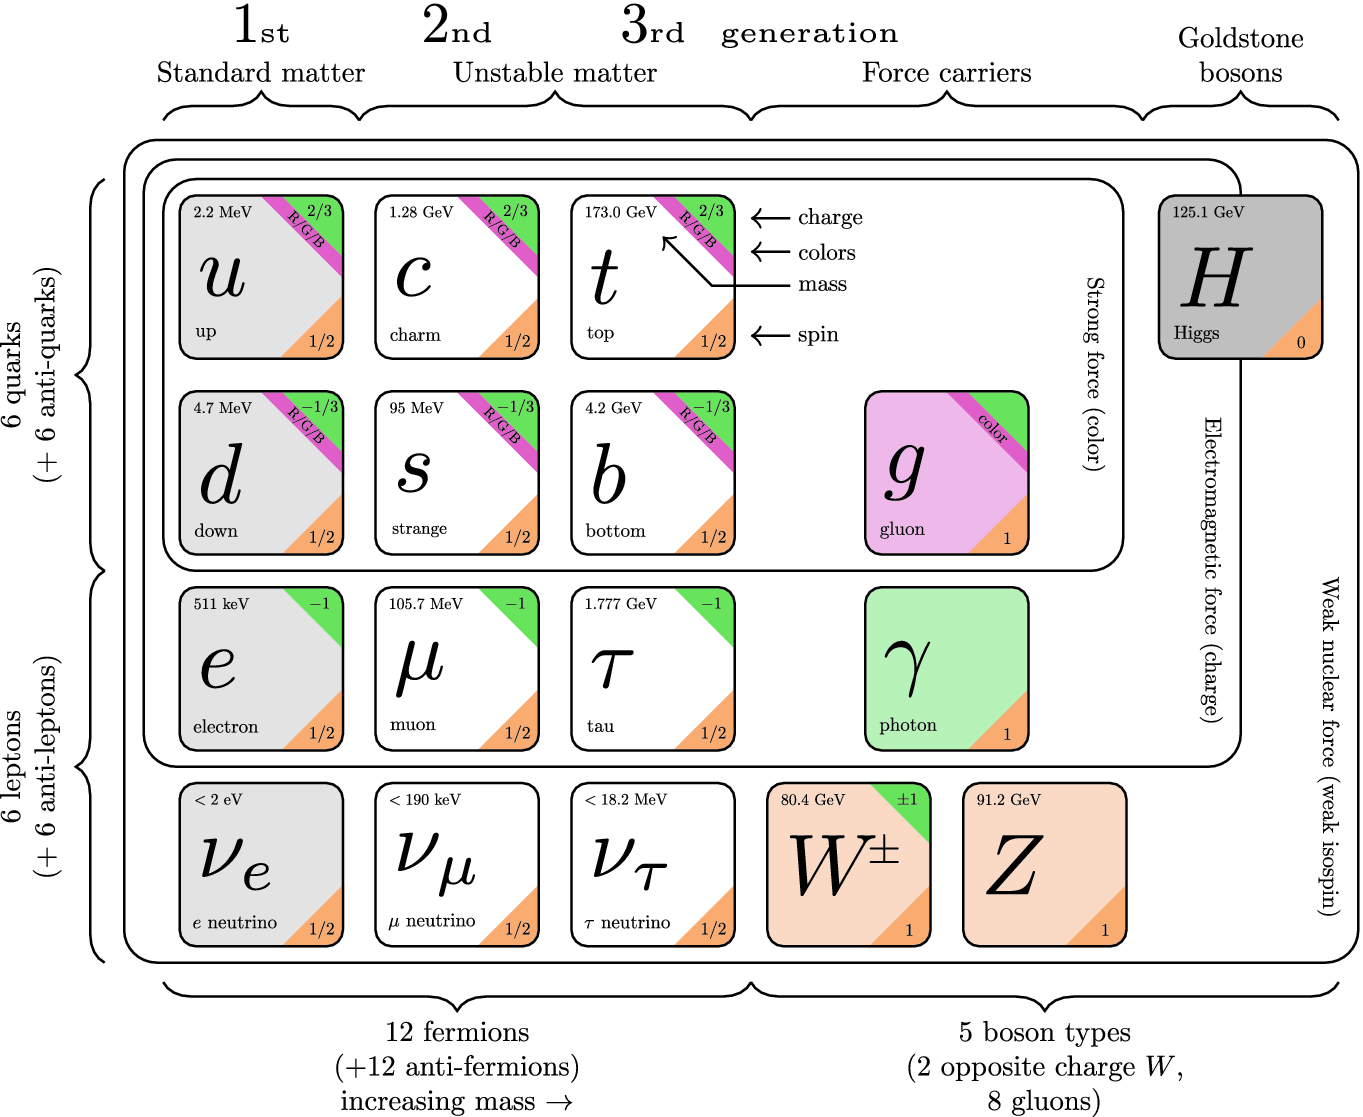
\includegraphics[width=8cm, height=6cm]{figs/SMFermions.png}
\caption{Representation of the 12 fermions of the \ac{SM} \cite{SMFermions} along with the main force carriers and the Higgs boson, discovered in 2012 and completing the \ac{SM}.}
\label{figure:SMFermions}
\end{center}
\end{figure}

The \ac{SM} Lagrangian density in a differential volume element $\mathcal{L} = \int L \text{ } d^3x$, accounting for the kinetic and potential energy of a system, takes the (very) simplified form given in Equation~\ref{eq:SMLag}, where $F_{\mu \nu}$ is the field strength tensor accounting for the different interactions, $\psi$ is the interacting field describing quarks and leptons and $\phi$ is the Brout-Englert-Higgs field while $y_{ij}$ are the Yukawa couplings to this field, which depend on the mass of the particle considered and which will be described later on in Section~\ref{subsection:ColliderProduction}.

\begin{equation}
\mathcal{L} = - \frac{1}{4} F_{\mu \nu} F^{\mu \nu} + i \bar{\psi} \cancel{D} \psi + \bar{\psi}_i y_{ij} \psi_j \phi + |D_\mu \phi|^2 - V(\phi)
\label{eq:SMLag}
\end{equation}

A complete description of this model is out of the scope of this work but it is important to note that the \ac{SM}, although mostly experimental, is still working extremely well today. Indeed, it managed to make a lot of predictions over the years, which is the best one can obtain from a mathematical model, and all of its major predictions revealed themselves to be true (we can quote for example that it successfully predicted the existence of the gluons, the top quarks, along with the W, Z and Higgs bosons \cite{SMPredictions}).

However, we know that the \ac{SM} is not the final theory of particle physics since it is not able to explain all the observations which have been made. There are some open questions and many \ac{BSM} theories trying to explain such observations, such as an eventual inclusion of the gravitational interaction within this model. We can quote for example as \ac{BSM} theories the possible existence of the supersymmetry, telling us that each particle should have a superpartner whose spin differs by 1/2 or the possible existence of \ac{DM} particles, the main subject of the following sections.

\section{At the origins of dark matter} \label{section:DMOrigins}

The origin of the concept of dark matter can be traced back to the 17 and 18th centuries, shortly after Newton's works on gravitation, even though this concept has changed quite a lot over the years. Back then, \ac{DM} was more considered to be ordinary matter which simply did not emit any kind of electromagnetic radiation, being therefore invisible and dark, but which does have a strong gravitation impact because of its mass. It was for example considered in the 20th century to be found in massive astronomical objects able to absorb the light or other objects located behind them, such as black holes \cite{Poincare}.

\subsection{Zwicky and the virial theorem}

In the 20th century, the first experimental evidences for the existence of dark matter were found. In 1933, Fritz Zwicky managed to determine the mass of the Coma Cluster using the virial theorem \cite{Zwicky}, which states that in a cluster in equilibrium under its own gravitation the kinetic energy must be comparable to its gravitational binding energy. 

Mathematically, the virial theorem can be written in Equation~\ref{equation:Virial}, where the brackets represent the mean value of the quantity obtained over time or position, the universal constant of gravitation is $G = 6.67 \cdot 10^{-11}$ m$^3$ kg$^{-1}$ s$^{-2}$ and where the gravitation potential energy expression can be simplified assuming a spherical distribution of the masses and the same average density everywhere in the cluster considered.

\begin{equation} \label{equation:Virial}
2 \langle T \rangle + \langle V \rangle = 0 \text{, where}
\begin{dcases}
T = \frac{1}{2} \sum_i M_i v_i^2 = \frac{1}{2} M \langle v^2 \rangle\\
V = -4 \pi G \int_0^R M \rho \text{ } r \text{ } dr \propto \frac{G M^2}{R}
\end{dcases}
\end{equation}

Solving these simple equations gives us an approximate value of the mass of the cluster in Equation~\ref{equation:ClusterMass}, where R is the radius of the cluster and $\langle \langle v^2 \rangle \rangle$ is the squared velocity of all the galaxies averaged over position and time.

\begin{equation} \label{equation:ClusterMass}
M \propto \frac{\langle \langle v^2 \rangle \rangle R}{G}
\end{equation} 

From this simple expression and astronomical observations, Zwicky then managed to compute the average mass to light ratio of its galaxies and concluded that the value obtained was around 400-500 times larger than the mass previously estimated by Edwin Hubble, who simply considered the number of visible galaxies within this cluster for his calculations. One plausible explanation for this discrepancy is to introduce the concept of \ac{DM}, which contributes to the mass of the cluster without increasing the galactic luminosity.

Zwicky's results were actually quite controversial since they were based on statistical calculations relying on different hypotheses not always justified, such as the fact that the galaxies in the cluster must be gravitationally bound with each other and they were actually proven to be overestimated later on \cite{ZwickyWrong}, but additional observations came to enforce the validity of his conclusions anyway.

\subsection{Spiral galaxies rotation curves}

Despite being controversial and slightly off, Zwicky's results were soon followed by a series of additional astronomical observations leading to the same conclusion, the possible existence of non-luminous matter in all the galaxies, called dark matter. The most famous of these results is the study of the observed and expected rotation curves of the stars within spiral galaxies such as the Milky Way in the 1970s \cite{RotationCurves}. 

According to this study, if we assume that we can apply Newton's universal laws of gravitation at the galactic scale, then the stars within this kind of galaxies should rotate with a velocity depending on the radius to the galactic center obtained by the usual equation for centripetal acceleration in a gravitational field and represented in Equation~\ref{equation:RotationVelocity}, where $M(r)$ accounts for the total mass encountered in a radius $r$.

\begin{equation} \label{equation:RotationVelocity}
v_{\text{rotation}}(r) = \sqrt{\frac{G M(r)}{r}}
\end{equation}

At first approximation, one can assume that most of the mass within this kind of galaxies comes from the inner core, which means that, at large radius, the velocity of individual stars is expected to decrease proportionally to $r^{-1/2}$. Any deviation to this rule suggests that either our understanding of gravity at large scales or our basic understanding of galaxies as a celestial body made of stars, dust and gas, has to be revised.

Actually, observations made by Vera Rubin and her team in the early 1970s with a new spectrograph designed to study the velocity curves of spiral galaxies with a degree of accuracy never reached before, did not confirm these expectations \cite{VeraRubin}. Indeed, according to these results, from a given value of the radius, the velocity curve appears to be flat instead of decreasing, as illustrated in Figure~\ref{figure:RotationCurves}. This is another hint that can motivate the introduction of the concept of \ac{DM}.

\begin{figure}[htbp]
\begin{center}
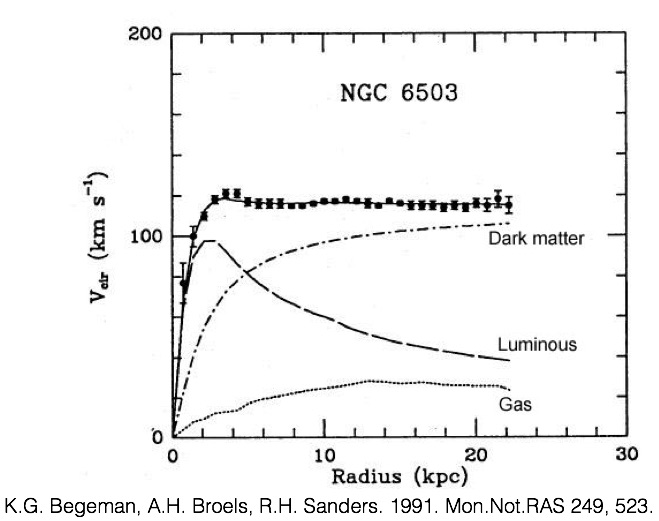
\includegraphics[width=8cm, height=6cm]{figs/RotationCurve.jpeg}
\caption{Expected and observed rotation curves of the galaxy NGC 6503 \cite{RotationCurves}. The black dots correspond to the data and the \textit{luminous} line corresponds to the rotation curve decreasing as $r^{-1/2}$ expected from Newtonian dynamics.}
\label{figure:RotationCurves}
\end{center}
\end{figure}

\vspace{-10pt}
\subsection{\acs{CMB} anisotropies} \label{subsection:CMB}

The \ac{CMB} is a mostly uniform background of primary radio waves emitted when the Universe became transparent around 380 000 years after the Big Bang and was discovered accidentally in the 1940s \cite{CMBDiscovery}. Studying it is extremely important, as it is actually made of the oldest and cleanest electromagnetic radiation we can find in the Universe. Precise measurements of this radiation are actually critical in many different fields of physics, since any proposed model of the Universe must be able to explain this radiation, its temperature and anisotropies. 

Recent measurements determined that the \ac{CMB} can be considered as emitting a thermal black body spectrum at a temperature of $(2.72548\pm 0.00057)$K \cite{CMBTemperature}. However, we now know that this temperature is actually not constant as some small anisotropies can be observed (at the $10^{-5}$ level), depending on the value of the solid angle of observation, as represented in Figure~\ref{figure:PlanckTemperature}.

\begin{figure}[htbp]
\begin{center}
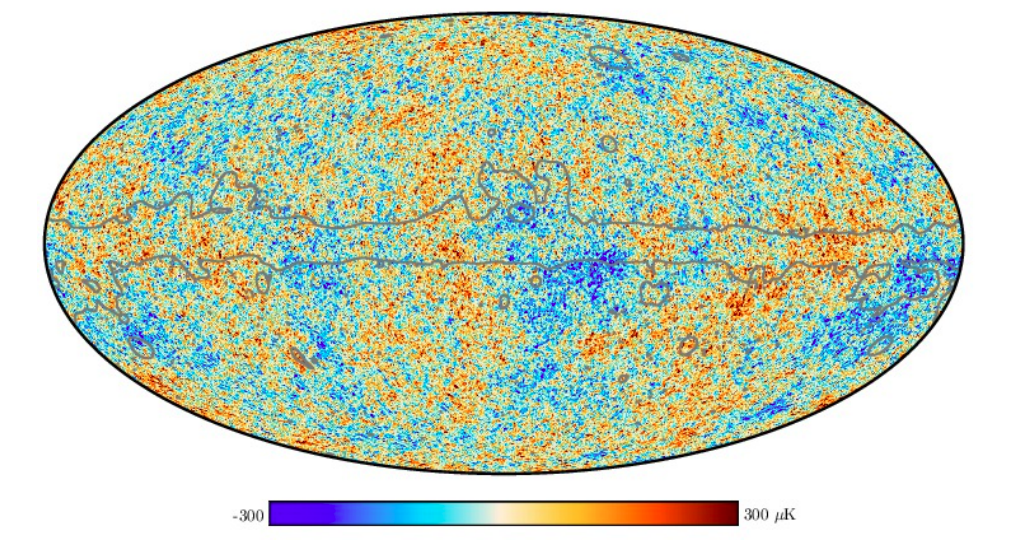
\includegraphics[width=14cm, height=6cm]{figs/PlanckTemperature.png}
\caption{Anisotropies at the $10^{-5}$ level in the temperature of the \ac{CMB}, as observed by the Planck satellite in 2018 \cite{PlanckTemperature}.}
\label{figure:PlanckTemperature}
\end{center}
\end{figure}


We see these fluctuations projected over a 2D sphere, and it is therefore natural to introduce at this point Laplace's spherical harmonics, $Y_{lm} (\theta, \phi)$, a complete set of orthogonal functions obtained by solving Laplace's equation $\nabla \psi = 0$ on a sphere and defined by a few parameters such as $l$, the multipole, representing a given solid angle in the sky ($l=100$ corresponds to $\sim 1\degree$) and $m$, the number of poles, such as $-l \leq m \leq l$ \cite{PowerSpectrum}. 

It is possible to show that these spherical harmonics form a complete orthonormal basis on this space and therefore that any function that can be defined on the sphere may be expanded into these harmonics using coefficients called $a_{lm}$. The temperature fluctuations, whose value depend on the two usual spherical angles $\theta$ and $\phi$ can therefore be expanded using these generic functions, according to Equation~\ref{equation:SphericalHarmonics}.

\begin{equation} \label{equation:SphericalHarmonics}
\frac{\Delta T}{T}(\theta, \phi) = \sum_{l=0}^{\infty} \sum_{m=-l}^{m=l} a_{lm} Y_{lm} (\theta, \phi)
\end{equation}

The information about the anisotropies can actually be extracted from the variance of these harmonic coefficients $a_{lm}$ of the expansion since the \ac{CMB} is assumed to be a Gaussian random field. The power spectrum of the \ac{CMB} can be extracted according to Equation~\ref{equation:PowerSpectrum}, and from which most of the cosmological information of the \ac{CMB} is derived.

\begin{equation} \label{equation:PowerSpectrum}
D_l = \frac{l(l-1) C_l} {2\pi} = \sum_m |a_{lm}^2|
\end{equation}

Interestingly enough, this spectrum is directly affected by the value of the density of the dark matter in the Universe, and this is something that will be often discussed in the remaining of this chapter. Doing a multi-parameters fit on the observed data represented in the power spectrum (cf. Figure~\ref{figure:CMBSpectrum}) is then able to give us directly the energy density of baryonic $\Omega_b$ and dark $\Omega_\chi$ matter, along with other important parameters of the $\Lambda_{CDM}$ cosmological model. Today's most precise measurements have been obtained in 2018 using the Planck satellite, and lead to the determination of these two quantities: $\Omega_b h^2 = 0.02220 \pm 0.00020$ and $\Omega_\chi h^2 = 0.1185 \pm 0.0015$ \cite{Planck}. This is one of the strongest constraint we have on \ac{DM} so far, since any \ac{DM} candidate will need to comply with this measurement.

By dividing these results with the value of the scaling factor for the Hubble expansion rate $h = 0.674$ \cite{Constants}, we can obtain from these numbers a proportion of 4.9\% of ordinary baryonic matter and 26.1\% of dark matter in the Universe.

\begin{figure}[htbp]
\begin{center}
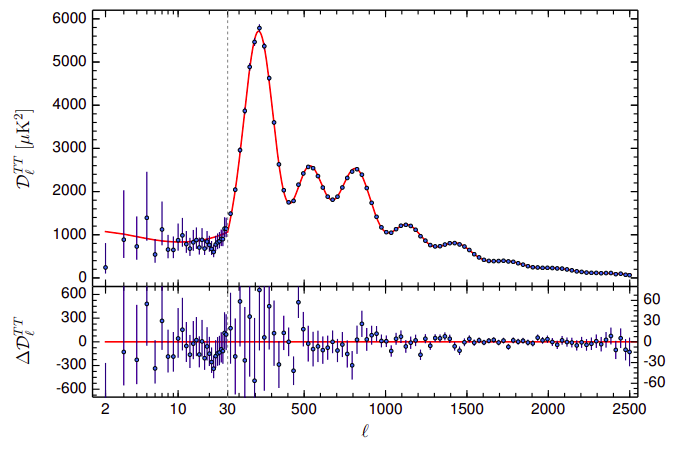
\includegraphics[width=10cm, height=6cm]{figs/PlanckSpectrum.png}
\caption{Power spectrum of the \ac{CMB} obtained by Planck, representing the fluctuations of the temperature of the radiation with respect to the angular angle of observation \cite{Planck}.}
\label{figure:CMBSpectrum}
\end{center}
\end{figure}

\subsection{Gravitational lensing}

The last evidence supporting the existence of dark matter has been obtained by observing several clusters of galaxies in the Universe, such as the Bullet Cluster, and by studying their mass distribution through gravitational lensing.

The gravitational lensing effect is a consequence of the general relativity, a theory developed by Einstein as a way to represent gravity using the geometry of space-time, stating that massive objects lying between distant sources and an observer should act as a lens and bend the light emitted by the source. This deviation of the light is actually proportional to the mass of the object in between the source and the observer, meaning that the gravitational lensing can give us a way to measure the mass distribution of massive objects, such as galaxy clusters. This mass distribution can then be compared to the luminous distribution of the cluster, to see if we can observe a discrepancy between the two measurements, which could be another hint of the existence of \ac{DM}.

The bullet Cluster is particularly interesting in this context since it actually provides an evidence for the eventual existence of \ac{DM} which does not rely on any mathematical assumption (other than the general relativity principle) and cannot at principle be explained by alternate laws of gravitation. In this case, some observations clearly showed that the spatial deviations between the center of the total mass and the center of the baryonic luminous mass cannot be explained with an alteration of the gravitational force law alone, with a statistical significance of $8 \sigma$ \cite{BulletClusterSigma}.

\begin{figure}[htbp]
\begin{center}
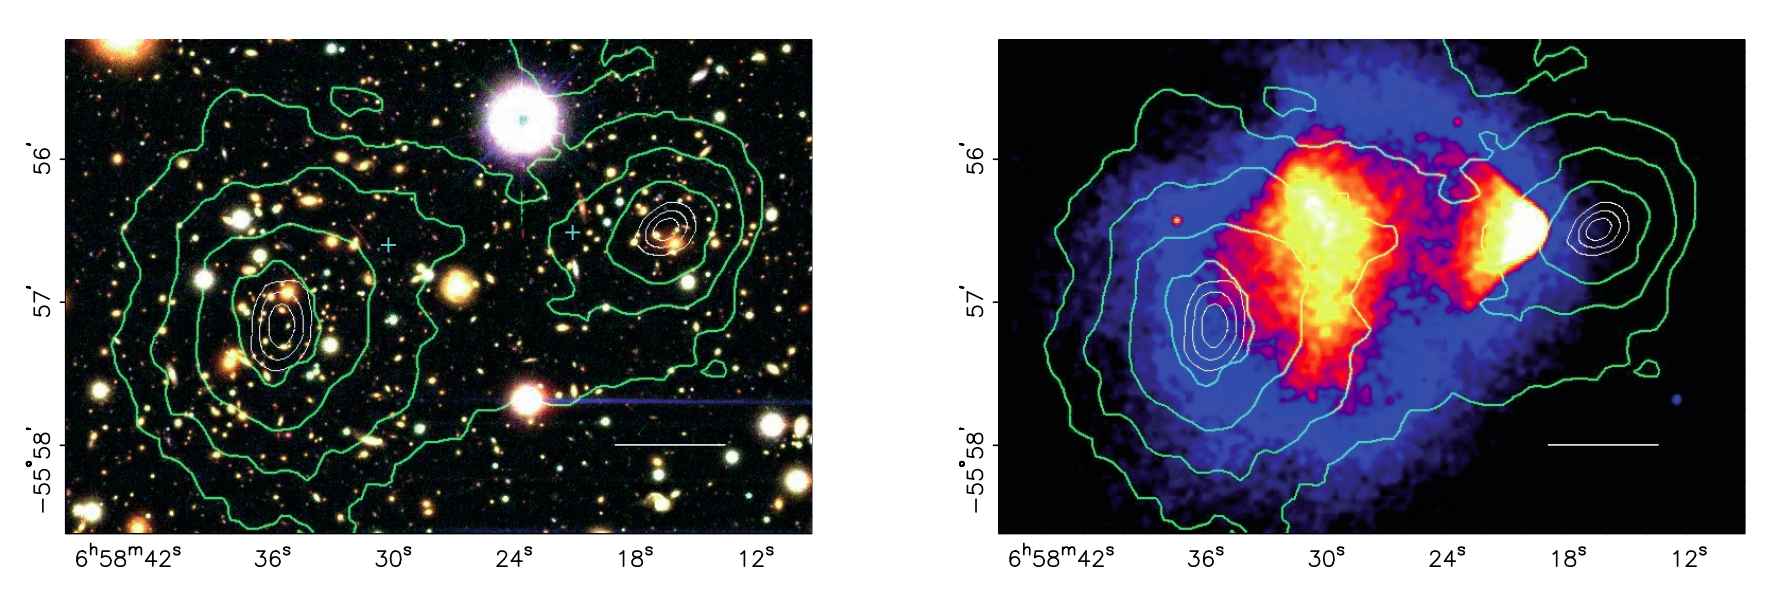
\includegraphics[width=14cm, height=6cm]{figs/BulletCluster.png}
\caption{Mass distributions obtained by the Magellan telescope in the visible (on the left) and the Chandra telescope on the X-rays spectrum (on the right) telescopes of the Bullet Cluser. Being shifted compared to each other, this is yet another clear evidence for the existence of \ac{DM} \cite{BulletClusterSigma}.}
\label{figure:BulletCluster}
\end{center}
\end{figure}

As seen in Figure~\ref{figure:BulletCluster}, the image taken by Chandra clearly shows an offset between the visible plasma of the cluster and the actual mass distribution measured through gravitational lensing (green contours). The center of the luminous mass of the cluster does not seem to match the one obtained considering its non-luminous counterpart as well, which is another evidence of the possible existence of \ac{DM} within galaxy clusters.

\section{Dark matter properties} \label{section:DMProperties}

All the previous observations allow us to list some of the most important properties that any dark matter candidate should have. Even though several theories exist, each giving slightly different properties to the \ac{DM}, we will consider in this work the following mostly accepted properties for such particles:
\begin{itemize}
\item First of all, we will assume that \ac{DM} is a \textbf{particle}. As far as we know, the Universe is simply composed of particles so there is no objective reason to think that \ac{DM}, being matter with a certain mass, might not be made of some kind of indivisible particles at some level.
\item Then, the \ac{DM} candidate should of course be \textbf{dark}. This means that it should not interact at all with electromagnetic radiation such as light, and that it should therefore be \textbf{electrically neutral}. However, it has to interact at least gravitationally because of the observations for the evidence of such a particle explained before, mostly relying on gravitational effects, and we assume in this work that it interacts weakly as well to have a chance to discover it with particle accelerators.
\item It has to be \textbf{non-baryonic}, mainly because the energy density for the baryonic matter obtained by observing the power spectrum of the \ac{CMB} is too low to account for \ac{DM} as well, as explained in Section~\ref{subsection:CMB}. Indeed, according to these results, baryonic matter accounts for around 5\% while dark matter accounts for more than 25\% of the energy density of the Universe. 
\item We will also only consider \textbf{cold} dark matter, since the widely accepted $\Lambda_{CDM}$ cosmological model is actually based on this assumption. By cold, we do not refer to the temperature of these particles but actually to their size, and therefore to the velocity by which they can travel in the Universe. Large scale structures of the Universe such as we can observe them today cannot actually be explained if \ac{DM} is made of hot/relativistic particles, as represented in Figure~\ref{figure:ColdWarmDM}. However, although not really as popular, it is important to note that alternative models with warm \ac{DM} have also been developed and still exist today.
\item It is interesting to report as well that \ac{DM} particles are expected to be found near the electroweak symmetry breaking scale, between \textbf{10 GeV and 1 TeV}. This is a consequence of the expected production mechanism of such particles, the so-called thermal freeze-out \cite{Freezeout1}. This principle tells us that at some point in history, \ac{DM} was supposed to be in thermal equilibrium with other primordial \ac{SM} particles, meaning that its production and annihilation rates were equal. However, because of the expansion of the Universe, at some point \ac{DM} particles were simply too far apart from each other and these reactions maintaining this equilibrium were not efficient enough any more. At this stage, the abundance of \ac{DM} became fixed: this is the freeze-out, as represented in Figure~\ref{figure:FreezeOut}.

%\begin{equation}
%\label{equation:equilibrium}
%\chi \bar \chi \leftrightarrow e^+ e^-, \mu^+ \mu^-, q \bar q, W^+ W^-, ZZ
%\end{equation}

This principle is interesting because, as a rule of thumb, we can say that if a particle interacts heavily, it will stay longer in equilibrium and its freeze-out abundance will therefore be smaller, so there is a mathematical relation between the strength of the \ac{SM}/\ac{DM} interaction $g$, the mass of the \ac{DM} particle $m_\chi$ and its relic abundance $\Omega_\chi$ that has been precisely measured, as expressed in Equation~\ref{equation:FreezeOut} \cite{FreezeOut}.

\begin{equation}
\label{equation:FreezeOut}
\Omega_\chi \propto \frac{m_\chi^2}{g^4}
\end{equation}

By using a typical value for $g$ of the order of the Fermi coupling constant $G_0^F \simeq 4.54 \cdot 10^{14}$ J$^{-2}$ we can see that, in order to observe a freeze-out abundance comparable to the one observed recently by the Planck satellite, the \ac{DM} candidate should have a mass between 10 GeV and 1 TeV as previously stated. The measurement of the \ac{CMB} power spectrum is therefore able to put constraints on the \ac{DM} cross-section with the baryonic sector, and all the \ac{DM} candidates quoted in Section~\ref{section:DMCandidates} will have to respect this criteria.

In any case, \ac{DM} is not expected to have a mass lower than 300 eV since at this scale, the phase space density that would be needed to explain the relic abundance of \ac{DM} would simply violate the Pauli-exclusion principle \cite{keVSterile}.

\item Finally, the \ac{DM} particles should be \textbf{long-lived}. Indeed, we expect that they were produced 13.8 billion years ago during the Big Bang, but it seems they are still present in the Universe since we still see their effect today. They should then be stable particles, or their lifetime should at least be larger than the age of the Universe itself.
\end{itemize}

\begin{figure}[htbp]
\begin{center}
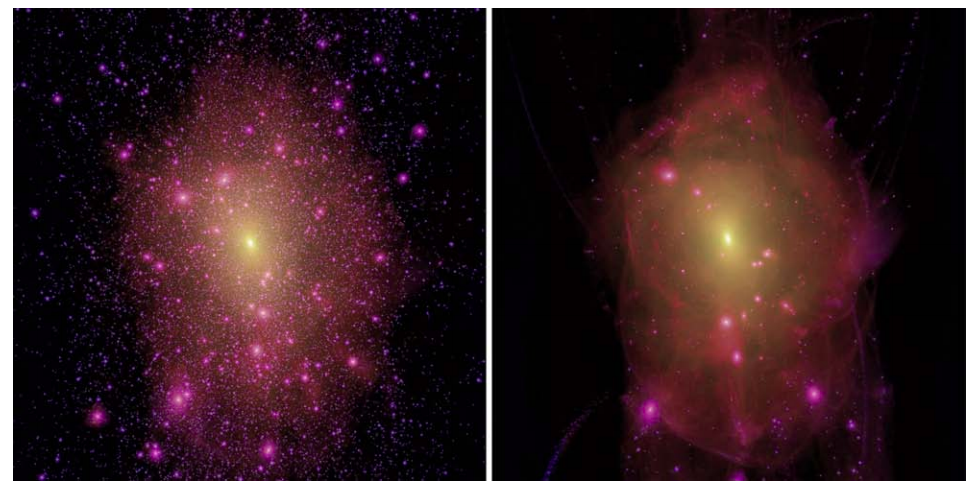
\includegraphics[width=14cm, height=6cm]{figs/ColdWarmDM.png}
\caption{Computer simulations for cold (on the left) and warm (on the right) \ac{DM} scenarios and their impact on a galactic halo at 0 redshift \cite{ColdWarmDM}.}
\label{figure:ColdWarmDM}
\end{center}
\end{figure}

\begin{figure}[htbp]
\begin{center}
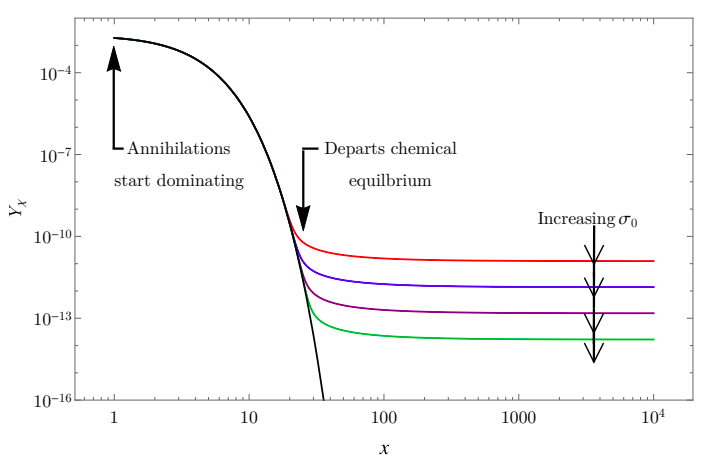
\includegraphics[width=10cm, height=6cm]{figs/FreezeOut.png}
\caption{Schematic representation of the freeze-out process, representing the abundance of a 500 GeV \ac{DM} as $Y_\chi$ with respect to the time and the impact of increasing cross-section annihilation values on this freeze-out abundance \cite{FreezeOut2}.}
\label{figure:FreezeOut}
\end{center}
\end{figure}

All these properties narrow quite a lot the number of possible \ac{DM} candidates.

\section{Dark matter candidates} \label{section:DMCandidates}

Several different categories of particles could pretend to be good candidates for dark matter but only the most interesting ones will be quoted here, since an extensive list of all the different possible candidates is out of the scope of this work. Two \ac{SM} particles will first of all be investigated, before introducing some \ac{BSM} theories providing additional \ac{DM} candidates with the expected properties.

\subsubsection*{\acfp{MACHO}}
The first obvious \ac{DM} candidates are the so-called \acp{MACHO}. These objects are massive astronomical non-luminous bodies (such as black holes) made of baryonic matter and very hard to detect, that could be responsible of the gravitational lensing observed and that could explain the apparent missing mass in the Universe. However, as we saw in Section~\ref{section:DMProperties}, \ac{DM} is not expected to be made of such ordinary matter, mainly because observational data of the \ac{CMB} and the deduced baryonic density of energy in the Universe is able to rule out this possibility.

Several different experiments did try to search for such \ac{DM} anyway, and managed to constrain the properties of this kind of objects. The main way to search for such massive objects is through their gravitational microlensing effect since, according to the general relativity principle, they should bend the light of luminous objects located behind them, such as stars, and this bending actually depends on the mass of the eventual \ac{MACHO}. Experiments like the \ac{MACHO} project and EROS observed in this context $\Theta (10^7)$ stars for several years, looking for microlensing events in order to constrain this particular \ac{DM} model. Results published in 2000 from the MACHO project, after studying almost 12 million stars, actually observed between 13 and 17 such events, lower than expected if \ac{DM} was only made of \acp{MACHO}. 

The collaboration actually managed to exclude at the 95\% \ac{CL} the possibility of the dark halo to be entirely made of such baryonic particles \cite{MACHOProject}. On the other hand, the EROS collaboration only observed 1 microlensing after studying more than 30 millions of bright stars during 6.7 years, while $\sim39$ events were expected \cite{EROS}. Both results have also been combined in order to obtain the exclusion plot represented in Figure~\ref{figure:ExclusionMACHO}. From this study, \acp{MACHO} with low masses of the order of a fraction of the mass of the Sum $M_\odot$ ($10^{-7}M_\odot < m < 10^{-3}M_\odot$) should make up less than 25\% of the dark matter halo for most models considered at the 95\% \ac{CL} \cite{ExclusionMACHO}.

\begin{figure}[htbp]
\begin{center}
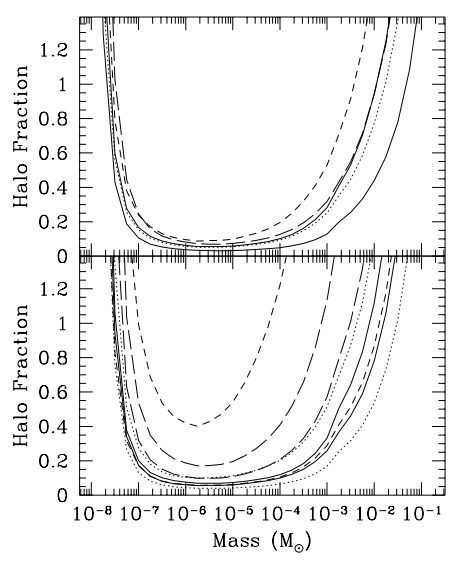
\includegraphics[width=6cm, height=8cm]{figs/MACHOExclusion.png}
\caption{Halo fraction upper limits at the 95\% \ac{CL} compared to the mass of the lensing object for different \ac{MACHO} models considered by the EROS (on the top) and the MACHO (on the bottom) collaborations \cite{ExclusionMACHO}.}
\label{figure:ExclusionMACHO}
\end{center}
\end{figure}

\subsubsection*{Active neutrinos}
\ac{SM} \textit{active} neutrinos $\nu$ (as opposed to \textit{sterile} neutrinos, that will be the subject of the discussion in the next section) have been considered as good \ac{DM} candidates for a long time as well, since they are electrically neutral and long-lived \ac{SM} particles, two important properties of any \ac{DM} candidate. They have a few particular properties that might be interesting in this context.

\begin{itemize}
\item First of all, even though it has still not been measured precisely, the sum of their masses has recently been measured to be lower than 0.17 eV at the 95\% \ac{CL} from cosmological studies \cite{NeutrinoMass}. Even though this is not fully understood, such value is incredibly low compared to other \ac{SM} particles, this particularity usually being referred to as the \textit{mass puzzle} of the neutrinos. 

\item Their low mass has a consequence in the sense that it means that the gravitational interaction between two neutrinos is usually considered to be negligible and that we can consider that they only interact weakly, making it hard to study their properties. Their actual cross-section of interaction, as represented in Figure~\ref{fig:NeutrinoXS} and which of course depends on their energies and on the channel of interaction (neutral or charged current considered), is therefore usually extremely low, making it hard to detect neutrinos.

\begin{figure}[htbp]
\begin{center}
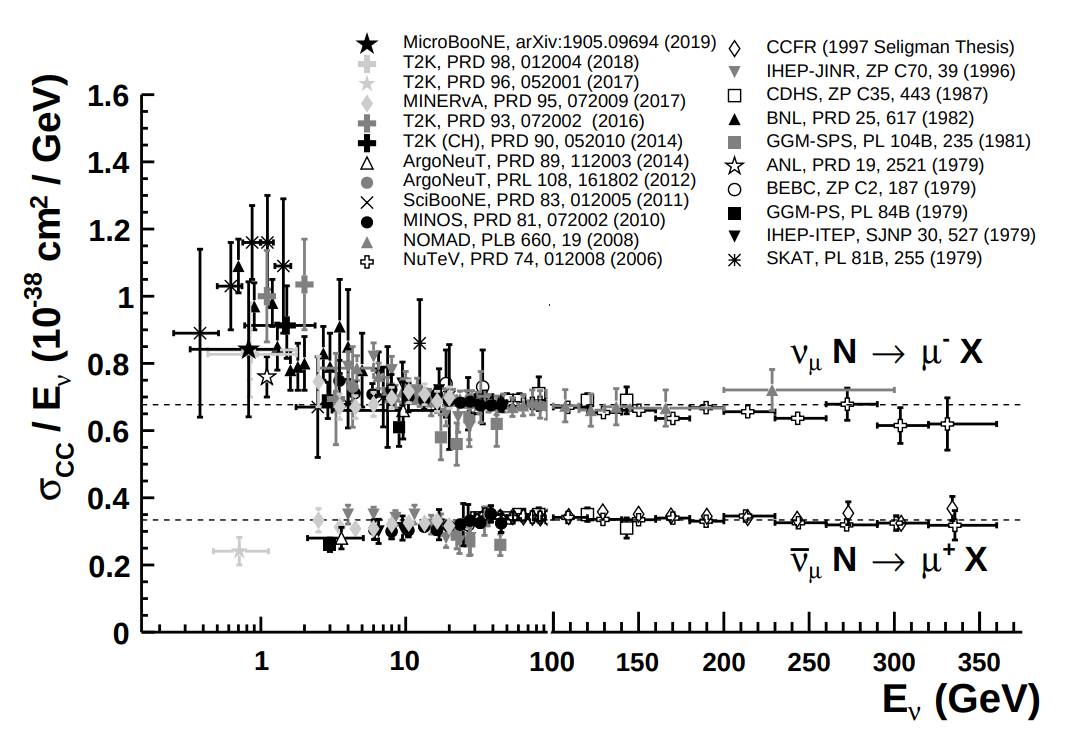
\includegraphics[width=12cm, height=8cm]{figs/NeutrinoXS.png}
\caption{Neutrino cross section of interaction from the charged current as measured by different experiments over a large range of energies, for both neutrinos $\nu$ and antineutrinos $\bar \nu$ \cite{PDGNeutrino}.}
\label{fig:NeutrinoXS}
\end{center}
\end{figure}

This figure clearly shows that an approximate value of the cross section for such neutrinos is of the order of magnitude of $10^{-38}$ cm$^2$ GeV$^{-1}$, which is typically tens of orders of magnitude lower than the interaction cross section of a photon ($\sigma_\gamma \sim 10^{-25}$ cm$^2$ \cite{GammaXS}). This means that the typical neutrinos of a few MeV produced by nuclear reactors have a mean free path of approximately 10 light years in steel.  

\item Neutrinos are also the only \ac{SM} particle only observed in their left-handed chirality state, while anti-neutrinos can only be observed in their right-hand state. This could mean two things: either right-handed neutrinos do not exist in nature for some reason, or we have just not been able to detect them because their interaction with baryonic matter is too weak. Right-handed neutrinos, also referred to as \textit{sterile} neutrinos, do not fit in the current \ac{SM} but could actually also be a strong \ac{BSM} \ac{DM} candidate, as we will discuss in the next subsection.
%\item Finally, neutrinos can oscillate, a quantum phenomena according to which the flavor of a neutrino can spontaneously change with time. This means that the three interacting states $\nu_\alpha$ observed are actually composed of several mass eigenstates $\nu_i$, as related in Equation~\ref{eq:Neutrinos}, where these states can be related using the Pontecorvo-Maki-Nakagawa-Sakata matrix $(V_\nu)_{\alpha i}$.

%
\end{itemize}

However, two physical reasons can explain why we do not really believe that \ac{DM} could be made of neutrinos any more. First of all, their relative abundance does not match the expected one for \ac{DM} from the freeze-out mechanism explained in Section~\ref{section:DMProperties}. Indeed, their freeze-out abundance can be computed quite easily from Equation~\ref{equation:neutrinoRelic} \cite{WIMPBook}, where the sum of the masses of the three neutrino flavors has been calculated to be lower than 0.17 eV \cite{NeutrinoMass} instead of the 11.5 eV expected to obtain the correct \ac{DM} relic abundance as observed today from the power spectrum of the \ac{CMB}. 

\begin{equation}
\label{equation:neutrinoRelic}
\Omega_\nu h^2 = \sum_{i=1}^3 \frac{m_{\nu_i}}{93 \text{ eV}}
\end{equation}

Additionally, for several reasons explained in Section~\ref{section:DMProperties}, a good \ac{DM} candidate is expected to be cold, i.e. non-relativistic. However, being extremely light, neutrinos are expected to be ultra-relativistic and could therefore not be responsible of the emergence of large scale structures as observed today. We can therefore most probably rule out the possibility of \ac{DM} being made of \ac{SM} neutrinos.

\subsubsection*{Sterile neutrinos}
The most obvious \ac{SM} particles being ruled out as \ac{DM} candidates, we can now introduce other \ac{BSM} theories introducing additional particles that could have the properties searched for. The first one of these theories introduces the so-called sterile neutrinos, usually referring to right-handed \ac{SM} neutrinos, as discussed in the previous subsection. 

If they exist, sterile neutrinos are expected to interact in an even weaker way than \ac{SM} active neutrinos, they could be very long-lived as well and in principle, nothing prevents us from considering that they could have a mass superior to 0.4 keV, giving therefore the correct \ac{DM} relic abundance \cite{keVSterile}. A superior bound of 50 keV on such particles can also be obtained considering limits on the observation of the monochromatic decay $\gamma$ line originating from the one loop radiative decay $N \rightarrow \nu + \gamma$ of such particles.

Several experiments are already searching for this kind of particles at this level of energy. Most of these experiments focus on the analysis of $\gamma$-rays and are actually searching for this particular monochromatic line resulting of the decay of sterile neutrinos. Two independent groups actually announced in 2014 the observation of an unidentified emission line at 3.57 keV (Figure~\ref{fig:DMDetection}) which did not match any known atomic emission line and which is actually consistent with an eventual \ac{DM} signal \cite{DMDetection1, DMDetection2}, since most of the possible instrumental contamination effects have been ruled out over the course of the last few years.

\begin{figure}[htbp]
\begin{center}
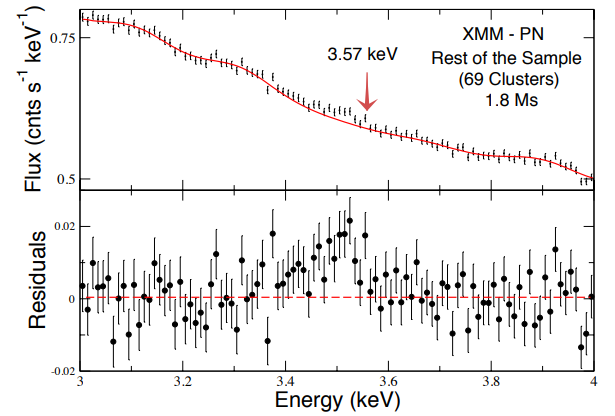
\includegraphics[width=8cm, height=6cm]{figs/DMDetection.png}
\caption{3.57 keV emission line detected with a $4.5 \sigma$ \ac{CL} by the XMM-Newton telescope in 2014, which could be a hint of the presence of \ac{DM} \cite{DMDetection1}.}
\label{fig:DMDetection}
\end{center}
\end{figure}

However, some additional studies of the galactic center pointed out the fact that this observation might actually come from the observation of a potassium K XVIII transition line \cite{NoDetection}. Recent observations actually ruled out at the 99\% \ac{CL} an eventual \ac{DM} origin for this particular line \cite{Nope}, but further studies are still ongoing.

\subsubsection*{Axions}
Axions could also explain the particle nature of \ac{DM}, since their existence is enough to explain 100\% of the \ac{DM} in the Universe, unlike most of the other candidates presented so far. Axions are hypothetical stable neutral particles, with masses of the order of the meV, introduced as a consequence of the strong-CP violation issue of \ac{QCD}. This issue is the following: the usual $\Theta$ term of the \ac{QCD} Lagrangian, the \ac{QCD} vacuum angle shown in Equation~\ref{equation:Lag} \cite{QCDLag} should be responsible of breaking the CP symmetry, but this effect has actually never been observed so far: this is the so-called the strong CP problem. 

Two ways to explain that we have never observed this phenomena exist: the first is to assume that one of the quarks of the \ac{SM} is massless but this does not match the current observations and measurements. The second consists in assuming that the parameter $\Theta$, the \ac{QCD} vacuum angle, is small enough so that this term becomes negligible. However, by definition, the $\Theta$ angle should be between 0 and $2\pi$, so there is no physical reason for this parameter to be small, unless some new physics can be introduced, such as the theory developed in 1977 by Peccei and Quinn \cite{Peccei} by relaxing $\Theta$ from a parameter to  a dynamic variable and absorbing it through the introduction of a new pseudoscalar particle that was called the axion.

\begin{equation}
\label{equation:Lag}
\mathcal{L}_\Theta = \frac{\Theta}{32 \pi^2} \epsilon_{\mu \nu \rho \sigma} G_a^{\mu \mu} G_a^{\rho \sigma}
\end{equation}

By definition, it is possible to show that axions satisfy two of the previous criteria for a good \ac{DM} candidate, since they are non-relativistic and their abundance might be enough to account for the dark matter energy density observed, because their actual abundance can easily be computed from Equation~\ref{equation:AxionDensity} \cite{AxionSearches}, from which we could conclude that an axion having a mass of $\sim$20 $\mu$eV could account for the \ac{DM} relic density of the Universe, as observed today. 

\begin{equation}
\label{equation:AxionDensity}
\Omega_a \simeq \left ( \frac{6 \mu \text{eV}}{m_a} \right )^{7/6}
\end{equation}

Several axion search experiments have therefore been set up, such as the \ac{ADMX}, a resonant microwave cavity installed at the University of Washington, the \ac{CAST}, a CERN experiment observing the Sun which came online in 2002 and which managed in 2014 to turn up definitely the existence of solar axions \cite{CASTLimit}, or the \ac{IAXO}, whose aim will be to search for axions with a much better signal to ratio noise than \ac{CAST}. All the results obtained by these experiments along with their future projections are represented in Figure~\ref{figure:AxionSummary}.

\begin{figure}[htbp]
\begin{center}
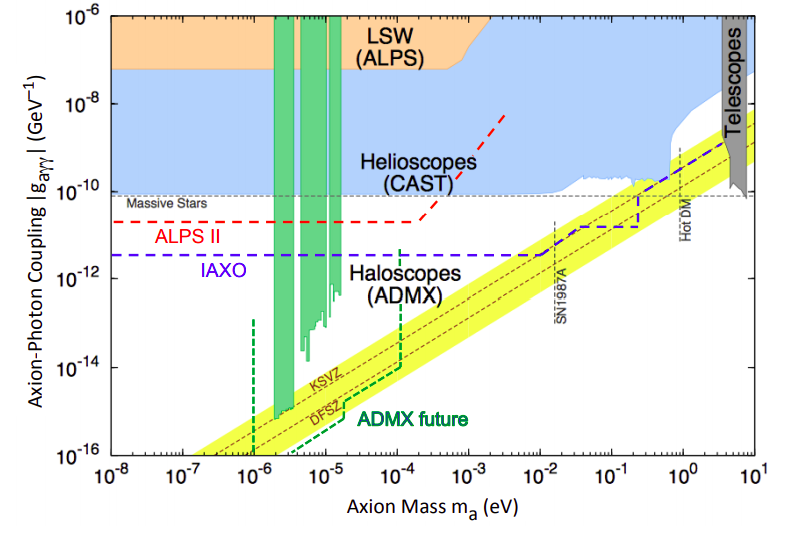
\includegraphics[width=12cm, height=8cm]{figs/AxionSummary.png}
\caption{Axions exclusion summary plot and projected coverage of axion searches experiments, such as \ac{ADMX}, \ac{CAST} and \ac{IAXO} \cite{AxionSearches}.}
\label{figure:AxionSummary}
\end{center}
\end{figure}

\subsubsection*{\acfp{WIMP}} 
The actual \ac{DM} candidates that will be mostly considered throughout this work are the so-called \acp{WIMP}, which are expected to interact, even though very weakly, with ordinary baryonic matter and which have an expected mass in the range of 100 GeV to 1 TeV for reasonable electroweak production cross-section values, right where we expect \ac{DM} to be found from its relic density: this is the so-called "WIMP miracle", an important concept that can be translated mathematically as well. Indeed, because of the freeze-out scenario explained in Section~\ref{section:DMProperties}, we can find an expression relating the relic abundance of \ac{DM} $\Omega_\chi$ with its annihilation cross section $\langle \sigma_A v \rangle$ through Equation~\ref{eq:Annihilation} \cite{IndirectSearches}.

\begin{equation}
\label{eq:Annihilation}
\Omega_\chi h^2 \sim \frac{3 \cdot 10^{-27} \text{ cm}^3 \text{ s}^{-1}}{\langle \sigma_A v \rangle}
\end{equation}

This equation implies that, since we do know the current abundance of \ac{DM} in the Universe, the total annihilation cross section of \ac{DM} should be equal to $\sim 3 \cdot 10^{-27} $ cm$^3 $ s$^{-1}$, which corresponds to the typical value given by \acp{WIMP} for a range of dark matter masses matching the expected one.

Several strategies can be used to detect such particles, as we will see in Section~\ref{section:DMSearches}. This kind of particle basically arises in various \ac{BSM} theories, such as the \ac{LSP} in SUSY. According to this theory, each \ac{SM} particle should have a superpartner whose quantum numbers would be identical except for their spins, which would differ by one half. All of these superpartners would then be potentially new and undiscovered particles, giving us a perfect \ac{DM} candidate in most of the \ac{MSSM} theories, the neutralino $\chi$ \cite{MSSM}.

The \acp{WIMP} are also interesting in the sense that introducing them in the terms of this supersymmetric theory would not only give us a strong \ac{DM} candidate, but would also solve the hierarchy problem, the apparent large discrepancy between multiple aspects of the weak and gravitational forces, such as their respective strength, differing by a factor $10^{24}$.

\section{Dark matter searches} \label{section:DMSearches}

As previously stated, several cosmological evidences allow us to introduce the concept of dark matter, but its properties such as its mass, coupling and interaction cross-section are difficult to study in this context. Several different ways can then be used to try and detect \ac{DM} particles in order to study them, as represented in Figure~\ref{fig:ThreeWays}, strategies which can usually be divided into three categories: the direct and indirect searches, mostly relying on the production of baryonic matter from the interaction between two \ac{DM} particles or on the observation of the interaction between the dark and baryonic sectors, and the production in colliders, usually able to probe lower \ac{DM} candidates masses and which will actually be the main focus of this work. 

%A discussion about these different detection strategies along with the main results obtained by different experiments in each case will now be presented.

\begin{figure}[htbp]
\begin{center}
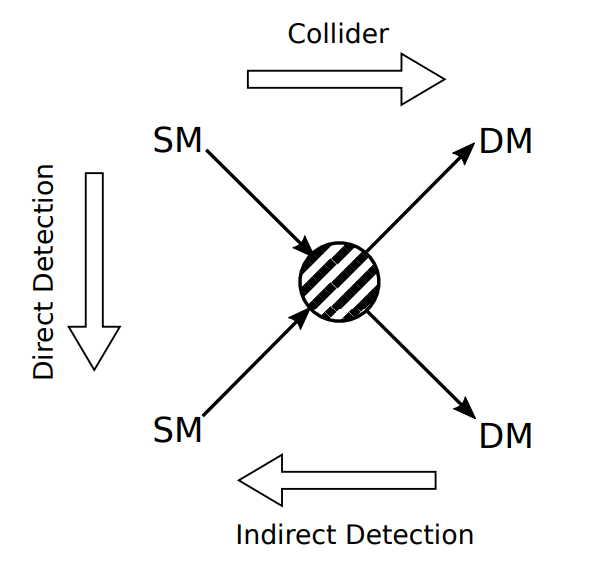
\includegraphics[width=5.5cm, height=5cm]{figs/ThreeWays.png}
\caption{Schematic view of the three main \ac{DM} detection strategies: direct, indirect and collider production searches \cite{ColliderSearches}.}
\label{fig:ThreeWays}
\end{center}
\end{figure}

\subsection{Direct searches} \label{subsection:DirectSearches}

From cosmological observations, we know that we live in a halo of dark matter. In this case, \ac{WIMP}s should cross the Earth every day and, even if they interact only weakly, we should be able to directly detect them through their interaction with ordinary baryonic matter, for example because of their scattering with the nuclei of the atoms. Indeed, the transfer of momentum between these two particles in this case might be detectable with the correct experimental device, typically placed deep underground to have the lowest possible background, which is the main source of perturbations of such experiments. 

To study this particular category of searches, let's first of all introduce the rate of expected WIMP scattering off a target nucleus of mass $m_N$ with Equation~\ref{equation:WIMPRate}, rate which ends up being described by a simple steeply
falling exponential function as shown in Figure~\ref{fig:DirectFalling} \cite{DirectSearches}, where $E_{nr}$ is the nuclear recoil energy measured, $m_\chi$ is the \ac{WIMP} mass, $\sigma$ its cross section, $\rho_0 = 0.3$ GeV cm$^{-3}$ is the local dark matter density and $f(v)$ the normalized \ac{WIMP} velocity distribution.

\begin{equation}
\label{equation:WIMPRate}
\frac{dR}{dE_{nr}} = \frac{\rho_0 M}{m_N m_\chi} \int_{v_{\text{min}}}^{v_{\text{esc}}} v f(v) \frac{d \sigma}{dE_{nr}}dv \propto \text{exp} \left (- \frac{E_{nr}}{E_0} \frac{4 m_\chi m_N}{(m_\chi + m_N)^2} \right )
\end{equation}

\begin{figure}[htbp]
\begin{center}
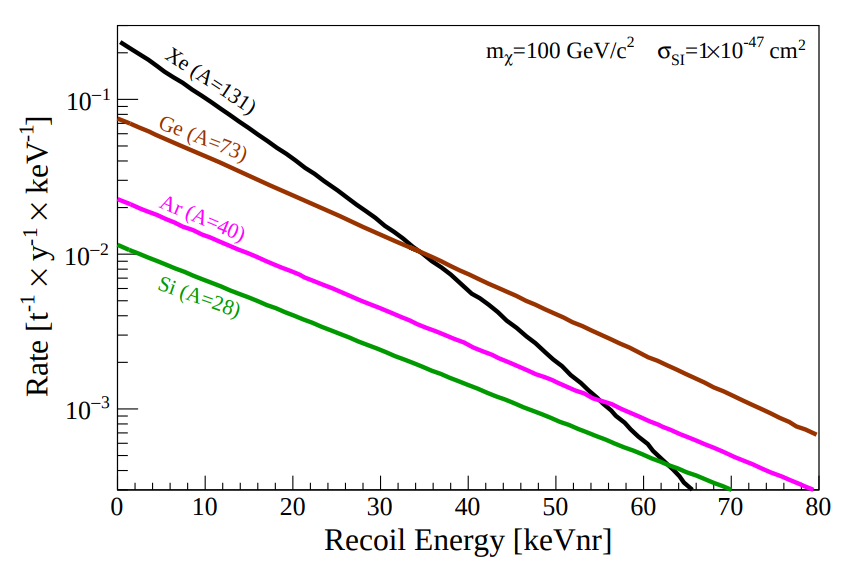
\includegraphics[width=10cm, height=7cm]{figs/DirectFalling.png}
\caption{ Nuclear recoil spectra induced in different materials for a given \ac{DM} \ac{WIMP} of 100 GeV, assuming a WIMP-nucleon \ac{SI} cross section \cite{DirectSearches}.}
\label{fig:DirectFalling}
\end{center}
\end{figure}

From this relation, the Equation~\ref{eq:Number} can be easily derived, representing this time the number of expected \ac{DM} events in an experiment running during a time $T$, where $\epsilon(E_{nr})$ is the efficiency of the detector for a given recoil energy.

\begin{equation}
\label{eq:Number}
N = T \int_{E_{\text{min}}}^{E_{\text{max}}} \epsilon(E_{nr}) \frac{dR}{dE_{nr}} \text{ } dE_{nr}
\end{equation}

The maximal velocity $v_{\text{esc}}$ used as superior bound of the integral in Equation~\ref{equation:WIMPRate} has actually been measured to be in the range $[498-608]$ km/s at the 90\% \ac{CL} \cite{EscapeVelocity}, since any particle having a velocity higher than this would not be bound any more to the gravitational potential of a galaxy. This has an important consequence: all the direct and indirect detection experiments actually need to take into account the annual modulation of the observed count rate, due to the movement of the Earth around the Sun, as shown in Figure~\ref{fig:AnnualModulation} \cite{AnnualModulation}, since this velocity is not negligible compared to the escape velocity $v_{\text{esc}}$. 

\begin{figure}[htbp]
\begin{center}
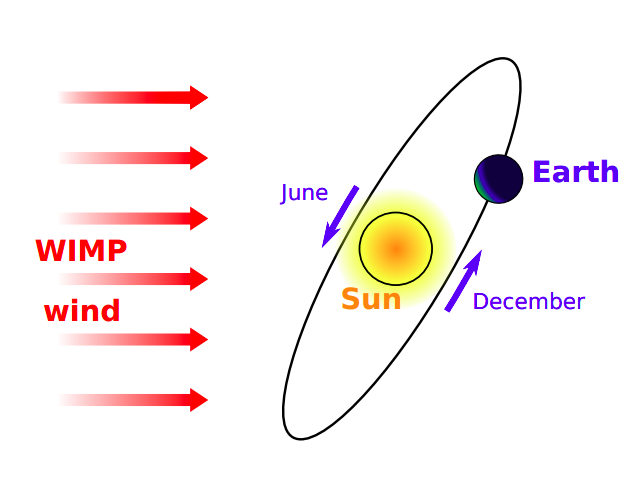
\includegraphics[width=8cm, height=6cm]{figs/AnnualModulation.png}
\caption{Schematic representation of the annual modulation of the WIMP wind introduced by the motion of rotation of the Earth around the Sun \cite{AnnualModulation}.}
\label{fig:AnnualModulation}
\end{center}
\end{figure}

From our perspective, it seems indeed that the velocity of the speed of \ac{WIMP} particles arriving is changing depending on the month of the year, since the Earth is sometimes moving in the direction of the \ac{WIMP} source, and is sometimes moving away: the maximal velocity is reached around June. It is extremely important to take into account this effect since, as we saw on the previous equations such as Equation~\ref{eq:Annihilation}, the count rate of incoming particles $N(t)$ actually depends on this velocity, and this modulation then introduces a periodical modulation that we need to take into account, as shown in Equation~\ref{eq:Modulation}, where the periodical part usually introduces a $\sim5$\% deviation \cite{DirectSearches}.

\begin{equation}
\label{eq:Modulation}
N(t) = B + N_0 + N_m \text{cos}(\omega (t-t_0))
\end{equation}

This effect is also important because an experiment performed during a long period of time can actually help us finding an eventual hint of \ac{DM} particles, since our signal is expected to follow this periodical deviation while the background is expected to be constant. Moreover, this \ac{WIMP} wind is expected to come from a particular region of the sky while the backgrounds are expected to be distributed uniformly, so this gives a clear way to isolate the signal.

Finally, it is also important to note that two different kinds of direct searches can be defined, depending on the category of the scattering between the \ac{DM} and the nucleus: the \acf{SI} (proceeding through the scalar term) and \acf{SD} (proceeding through the axial term of the Lagrangian) searches, since the interaction cross section $\sigma$ of Equation~\ref{equation:WIMPRate} is expected to be different for \ac{DM} particles having a spin 0 or not, as shown in Equation~\ref{eq:SISD}, where $F$ is a factor accounting for the dependence of the scattering on the energy. This means that results obtained by either hypothesis cannot be compared with each other.

\begin{equation}
\label{eq:SISD}
\frac{d\sigma}{dE_{nr}} \propto \sigma_{SI} F_{SI}^2(E_{nr}) + \sigma_{SD} F_{SD}^2(E_{nr})
\end{equation}

As previously stated, many experiments are dedicated to the direct search of \ac{DM} particles, but in order to isolate an eventual \ac{DM} signal, an environment with an ultra-low background is usually required, which is usually reduced either by placing the detector underground (to reduce the contamination due to cosmic rays), by increasing the statistics (by repeating the experiment and/or observing for a larger amount of time) or by choosing carefully the active material of the detector (to reduce the internal background coming from the detector itself). The impact these kind of parameters have on the final limits can be seen in Figure~\ref{fig:ImpactLimit}.

\begin{figure}[htbp]
\begin{center}
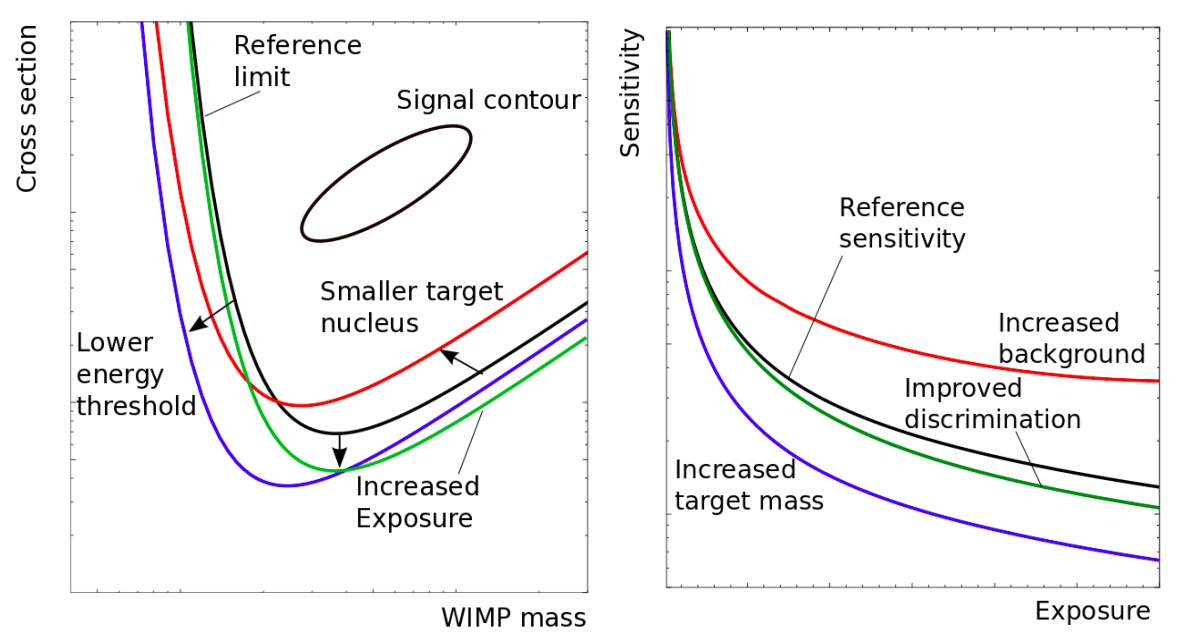
\includegraphics[width=14cm, height=7cm]{figs/ImpactLimits.png}
\caption{Impact of different experimental parameters on the final limits depending on the cross section and \ac{WIMP} mass (on the left) or sensitivity and exposure (on the right), with respect to the expected limits (black curve) \cite{DirectWays}.}
\label{fig:ImpactLimit}
\end{center}
\end{figure}

These detectors try to detect the scattering of an unknown exotic particle with an ordinary nucleus, which typically can give rise to different categories of signals. Some detectors try for example to detect the direct ionization of the target atom, while others focus on the emission of light coming from the de-excitation of the scattered nucleus, and some even search for the heat produced by these collisions under the form of phonons (collective excitation phenomena in condenses matter) in a crystal. These different search strategies have been summarized schematically in Figure~\ref{figure:DirectWays}.

\begin{figure}[htbp]
\begin{center}
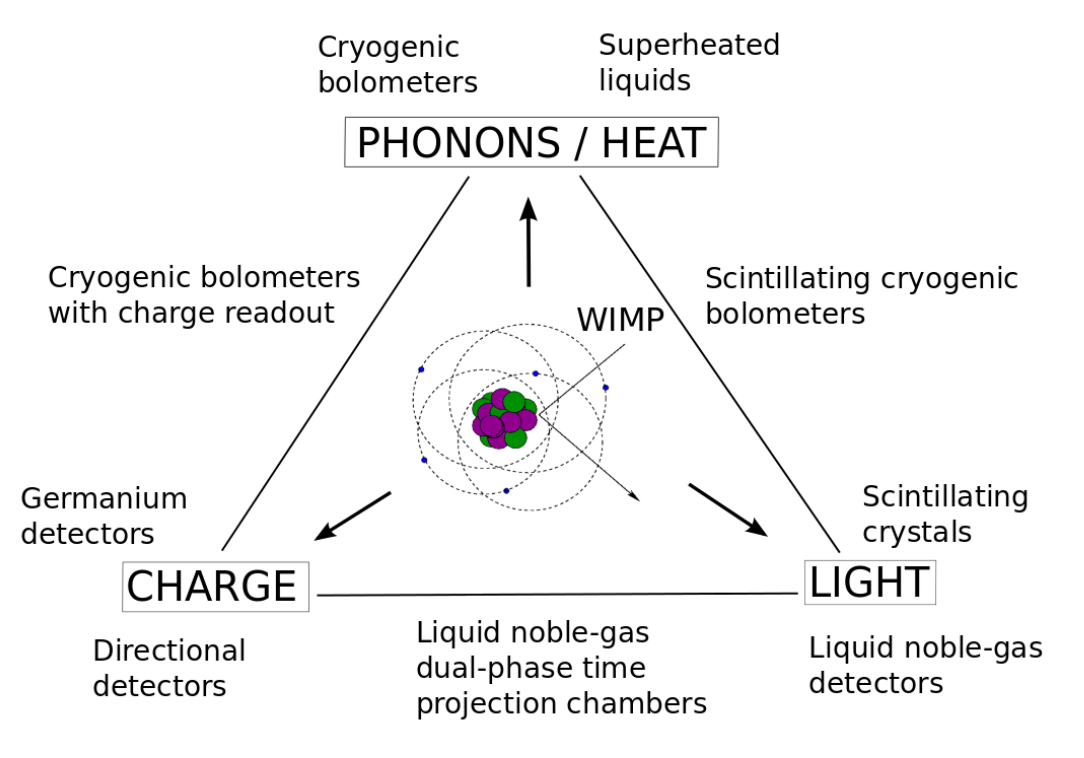
\includegraphics[width=12cm, height=8cm]{figs/DirectWays.png}
\caption{Schematic representation of the three main strategies to detect directly the interaction between \ac{DM} particles and an ordinary nucleus \cite{DirectWays}.}
\label{figure:DirectWays}
\end{center}
\end{figure}

As of today, no direct experiment has been able to detect serious hints for the existence of \ac{DM}, and they have only been able to set limits on the scattering cross section depending on the models parameters, as seen in Figure~\ref{fig:DirectLimits} for multiple experiments at once.

\begin{figure}[htbp]
\begin{center}
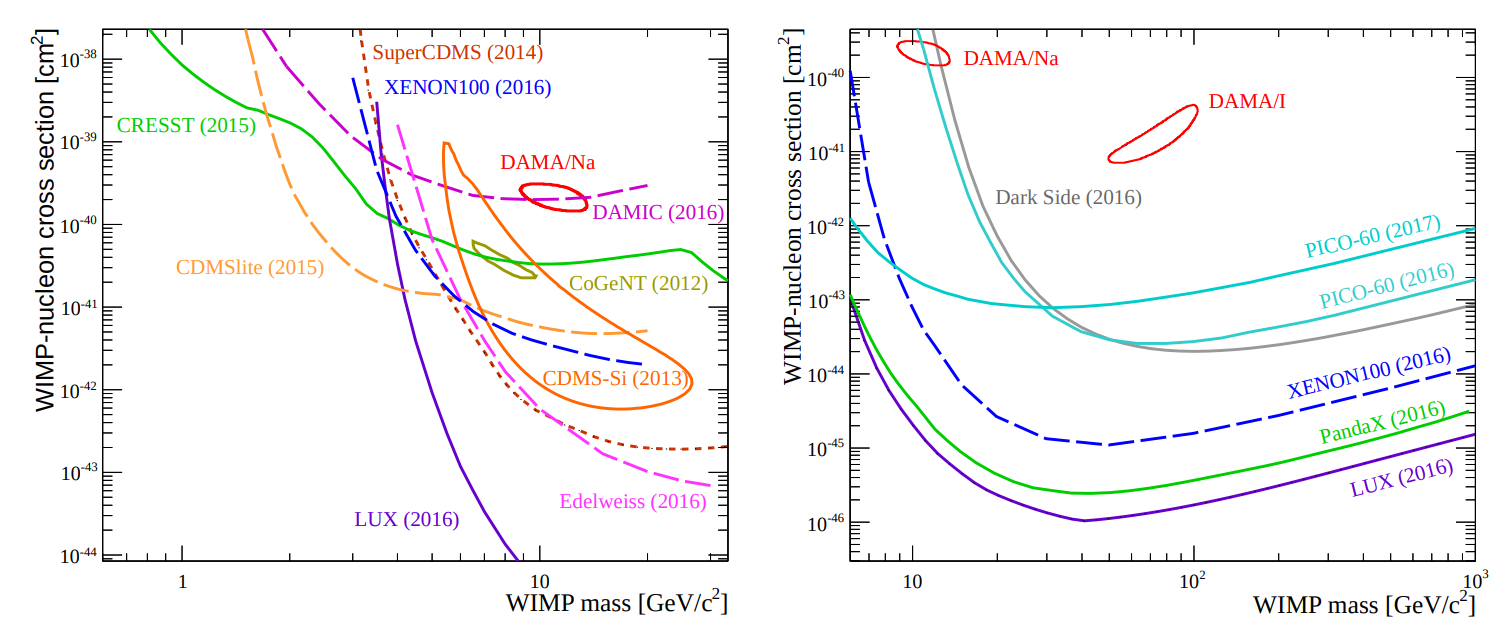
\includegraphics[width=14cm, height=6cm]{figs/DirectLimits.png}
\caption{Exclusion limits obtained by various direct detection experiments considering a \ac{SI} interaction cross section for low \ac{WIMP} (on the left) or high \ac{WIMP} masses (on the right) \cite{DirectWays}.}
\label{fig:DirectLimits}
\end{center}
\end{figure}

However, the DAMA experiment at the \ac{LNGS} did find an interesting result by showing the hints of an annual modulation signal compatible to the expected one due to the \ac{WIMP} wind in the 2-6 keV energy range, as seen on Figure~\ref{fig:DAMA} \cite{DAMA}. Further investigations about this modulation are still ongoing today, since no systematic effect able to account for the observed modulation amplitude and to simultaneously satisfy all the requirements of the signature has been found so far.

\begin{figure}[htbp]
\begin{center}
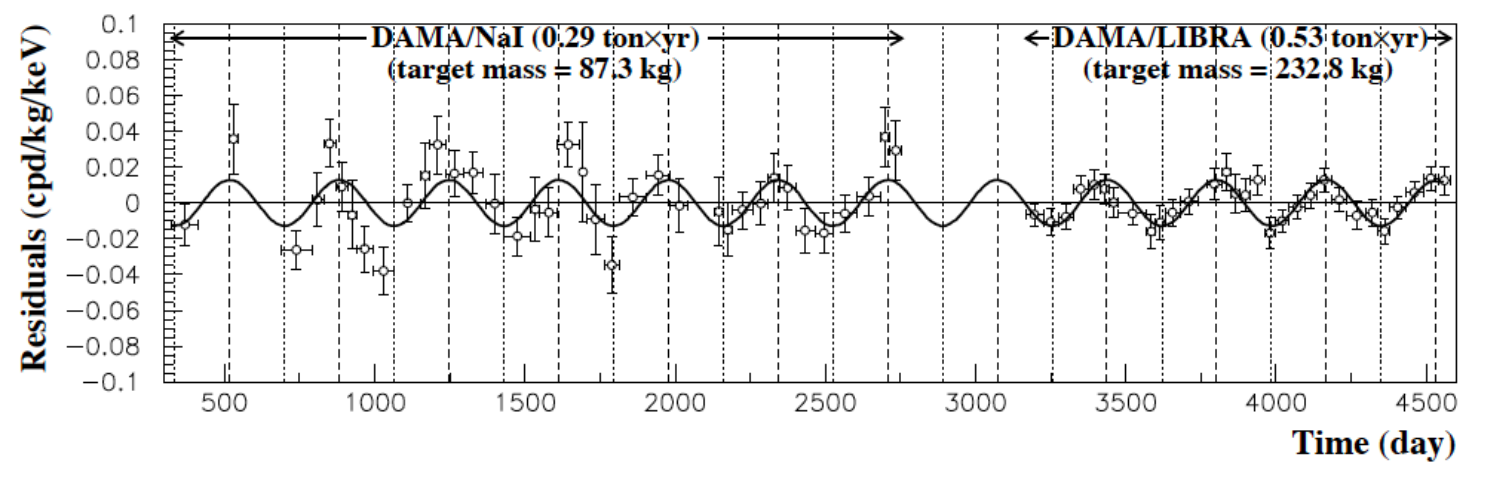
\includegraphics[width=14cm, height=5cm]{figs/DAMA.png}
\caption{Observed and expected annual modulation in single hits events in the 2-6 keV energy range by the DAMA experiment \cite{DAMA}.}
\label{fig:DAMA}
\end{center}
\end{figure}

\subsection{Indirect searches}

The indirect detection of \ac{DM} particles consists basically in searching for \ac{SM} products coming from the annihilation of two \ac{DM} particles or from its eventual direct decay, usually under the form of a flux of $\gamma$-rays, neutrinos, cosmic-rays or anti-matter appearing as an excess over the expected background. Indeed, many extensions to the \ac{SM}, such as the supersymmetry SUSY or \ac{UED} do provide solid \ac{DM} candidates (the lightest supersymmetric particle and the lightest Kaluza-Klein state, respectively) expected to interact with each other, resulting in the immediate production of \ac{SM} (un)stable particles that can be detected by telescopes either placed on the ground or directly in space. Another point to make is that indirect searches are also usually affected by the annual fluctuation induced by the movement of the Earth around the Sun, as explained in Section~\ref{subsection:DirectSearches}.

Indirect searches are actually extremely useful since they are sensitive to the \ac{DM} annihilation cross section, mass and the density profile of \ac{DM} halos $\rho(\overrightarrow{r}(s, \Omega))$, usually represented by a \ac{NFW} profile, as shown in Equation~\ref{eq:NFW}, where $r_s = 20$ kpc is the scale radius of the \ac{DM} halo for the Milky Way and $r$ is the distance to the center of the cluster considered, assumed to be spherical in this case \cite{FluxIndirect}.

\begin{equation}
\label{eq:NFW}
\rho(r) \propto \frac{r_s}{r \cdot \left (1+\big (\frac{r}{r_s} \big)^2 \right )}
\end{equation} 

The flux coming from the annihilation of two \ac{DM} particles is then expected to be proportional to its annihilation cross section $\sigma v$, the solid angle of observation $\Omega$ and the number of particles emitted by this annihilation $\frac{dN}{dE}$, according to Equation~\ref{eq:FluxIndirect}, where the integration is done over the line of sight $l$ and the solid angle of observation $\Omega$.

\begin{equation}
\label{eq:FluxIndirect}
\frac{d \Phi}{d\Omega dE} = \frac{\sigma v}{8 \pi m_\chi^2} \cdot \frac{dN}{dE} \iint_{l, \Omega} \rho^2(\overrightarrow{r}(s, \Omega)) \text{ } dl \text{ } d\Omega \equiv P \cdot J(\Delta \Omega)
\end{equation} 

This equation is extremely important for two reasons. First of all, it shows that, if a signal is found in direct detection, we could use this detection to determine the new object mass and scattering cross section and then use this information in order to obtain the \ac{DM} density profile this way: the data obtained by the different strategies of detection are actually complementary. The second reason is that as we can see, the flux of incoming particles can actually be divided into two factors: $P$, entirely dependent on the physics of the \ac{DM} particle, and the $J$-factor $J(\Delta \Omega)$, depending only on the distribution of \ac{DM} within the system considered. This $J$-factor is in this sense actually a measurement of the quality of an astronomical object for an indirect measurement, since the higher the flux received, the better the measurement will be in general (even though this is not the only factor which matters, since for example the galactic center has a higher $J$-factor than the best dwarf galaxy observable, but also has a lot of backgrounds affecting the measurement).

As different channels of observation are available for us to analyze the eventual annihilation of \ac{DM}, several strategies can be used in order to detect \ac{DM} indirectly, by searching different kinds of \ac{SM} particles. Anyway, all these strategies have one goal in common: try to reduce the background, since the signal searched for is usually quite low while the uncertainties associated to the background in astrophysics are usually quite high.

\subsubsection*{Through $\gamma$-rays detection}
The golden channel for such searches is through the production of $\gamma$-rays by \ac{DM} annihilation $\chi \chi \rightarrow \gamma + X$ or decay $\chi \rightarrow \gamma + X$, mainly because the energy scale of the \acp{WIMP} implies that most of the annihilation and decay radiation will be emitted in this range of energies and because $\gamma$-rays are usually not deflected when traveling to the observer (this means that the exact source of this kind of radiation can be quite easily and precisely pin-pointed). However, they do have one drawback as well: the Earth's atmosphere is usually opaque to this kind of radiation at this level of energy. This means that most of experiments searching for them simply cannot be performed from the ground and have to be sent to space. 

One of the most famous detectors in this category is the \ac{LAT}, a pair production detector launched in June 2008 and mostly sensitive to $\gamma$-rays between 20 MeV and 300 GeV \cite{LATExperiment}. This experiment has managed to exclude a large portion of the phase space, as seen in Figure~\ref{figure:LATExclusion}. The GAMMA-400 experiment, whose launch is scheduled in 2020, will pick up the work of \ac{LAT}, by studying a similar range but with much improved angular and energy resolutions \cite{GAMMA400}. 

\begin{figure}[htbp]
\begin{center}
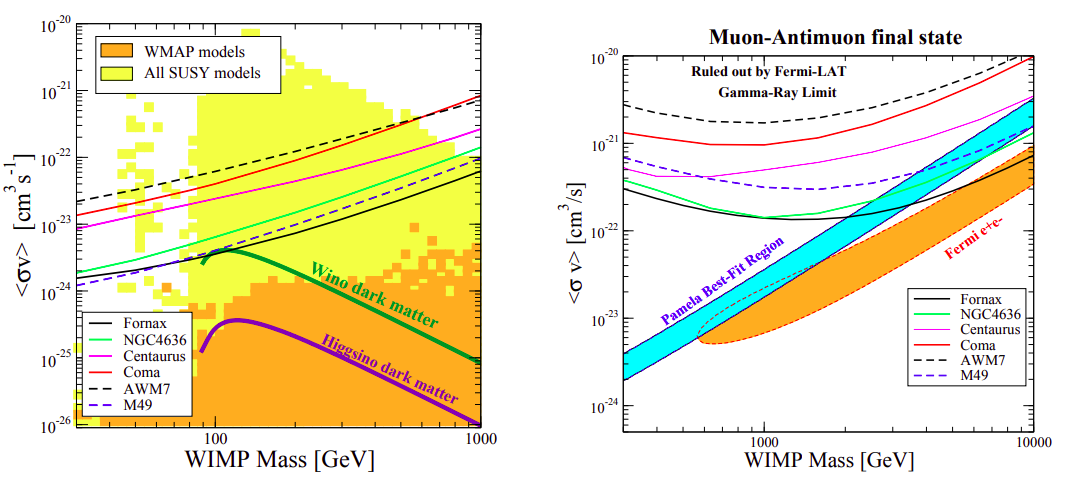
\includegraphics[width=12cm, height=6cm]{figs/LATExclusion.png}
\caption{Upper limits on the \ac{DM} annihilation cross section considering $b \bar b$ (on the left) and $\mu^+ \mu^-$ (on the right) final states as a function of the \ac{WIMP} mass, for different clusters studied \cite{LATExperiment}.}
\label{figure:LATExclusion}
\end{center}
\end{figure}

It is much harder for \ac{DM} to produce high energy $\gamma$-rays and therefore, the flux of such particles decreases quite quickly with energy, making it harder to study since telescopes then need a much larger effective area to pick up the same quantity of signal, and have therefore to be put on the ground. Such telescopes do exist, are called \ac{IACT} and have to take into account the atmospheric perturbations to work in an optimal way. They are usually sensitive to a range of energies going from $\sim 10$ GeV up to $\sim 100$ TeV, but can usually only study a small portion of the sky (up to a few degrees), forcing these experiments to choose carefully the objects to be studied. The \ac{CTA} is a brand new telescope of this kind whose construction is supposed to start in 2020, that should improve greatly the sensitivity of high masses indirect \ac{DM} searches.

\subsubsection*{Through neutrinos detection}
Interacting only weakly, neutrinos are another reliable source of data in the Universe since they are not supposed to be altered when traveling large distances as well, even though detecting neutrinos is much harder than detecting $\gamma$-rays and usually involves huge tanks of water in which neutrinos can be detected with the Cherenkov effect, which consists of the emission of an electromagnetic radiation when a charged particle moves through a dielectric medium with a speed greater than the speed of light in this medium.

The most famous detector of this kind, the IceCube neutrino observatory, actually uses the ice of the South Pole instead of water to detect these particles with photo-detectors, mainly because of the low interaction cross section of the neutrinos which then requires the installation of a huge volume of material to increase the probability of interaction. Super-Kamiokande (Super-K), in Japan, is another large Cherenkov experiment dedicated to the detection of cosmic neutrinos. Both detectors are also largely involved as direct searches experiments, since they are also sensitive to the eventual recoil between \ac{DM} and ordinary matter nuclei.

The problem with this kind of experiment is the difficulty of actually detecting some neutrinos, along with the background levels from atmospheric neutrinos, as represented in Figure~\ref{fig:BkgNeutrino}, typically several orders of magnitude larger than the signal. Multiple strategies therefore need to be put in place in order to reduce the background level in such experiments, such as the study of the directionality of the source and an appropriate choice of angle of observation, since most of the contamination is coming from tau neutrinos, themselves originating from muon neutrinos oscillation, strongly suppressed around the zenith.

\begin{figure}[htbp]
\begin{center}
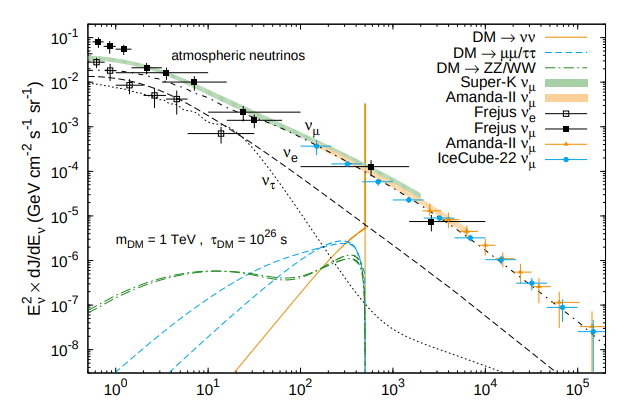
\includegraphics[width=12cm, height=8cm]{figs/BkgNeutrino.png}
\caption{Neutrino spectra for a scalar \ac{DM} candidate of 1 TeV for different indirect detection experiments and the corresponding background level expected \cite{BkgNeutrino}.}
\label{fig:BkgNeutrino}
\end{center}
\end{figure}

\subsubsection*{Through cosmic rays detection}

Searching for anti-matter in the cosmic rays presents the advantage of being highly sensitive, because of the low levels of backgrounds this kind of searches implies. However, cosmic rays are affected when traveling through the Universe, and determining the exact location of their emission can be quite challenging.

Among the most famous detectors of this kind, we can quote PAMELA, a spatial telescope dedicated to the study of such cosmic rays since 2006. \ac{CERN}'s \ac{AMS}, installed in the International Space Station has also studied such radiation from a range of a few hundred MeV up to 1 TeV. The data collected by this detector is compared to the exclusion limits obtained by the IceCube detector in Figure~\ref{fig:AMSData}.

\begin{figure}[htbp]
\begin{center}
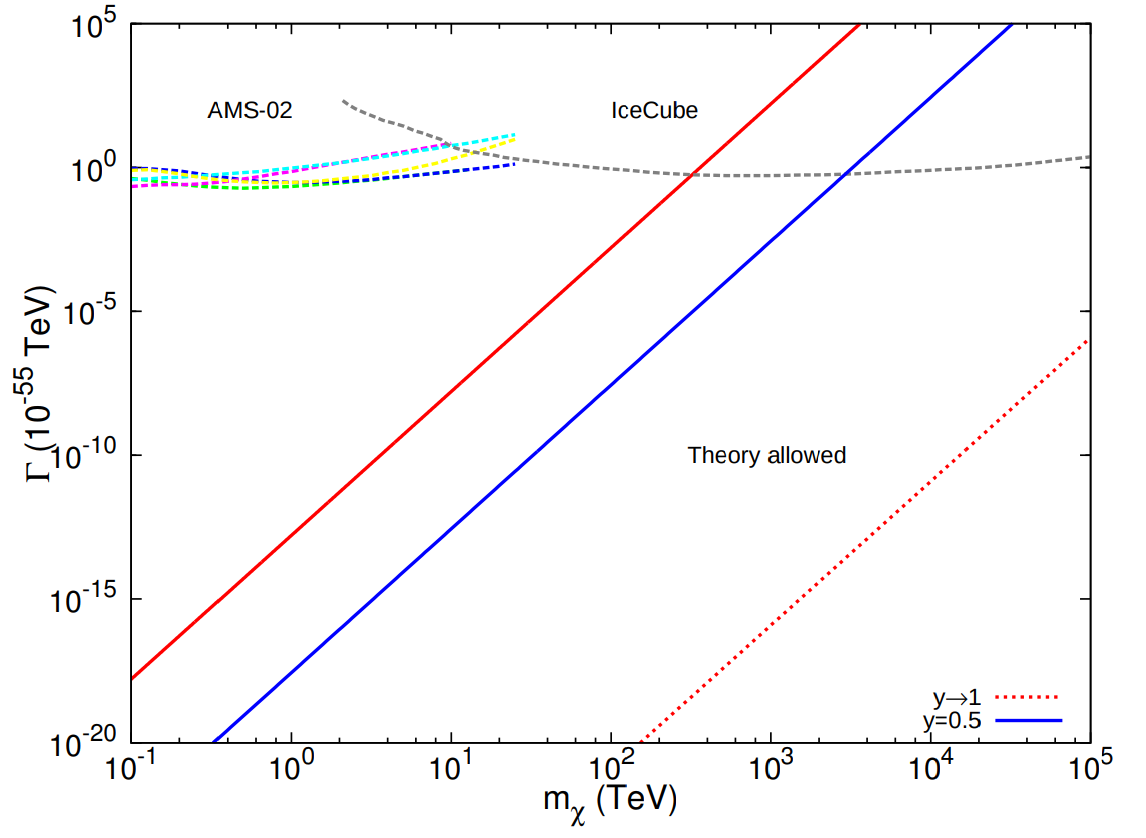
\includegraphics[width=10cm, height=7cm]{figs/AMSData.png}
\caption{Limits of the decay width of the interaction with respect to the \ac{DM} mass obtained by both IceCube and \ac{AMS} \cite{AMSData}.}
\label{fig:AMSData}
\end{center}
\end{figure}

\subsection{Collider production} \label{subsection:ColliderProduction}

In this particular kind of searches, we are interested in the eventual direct production of \ac{DM} candidates following the collision between two highly energetic \ac{SM} particles, a perfectly viable scenario if we keep assuming that \ac{DM} should at least interact weakly with ordinary matter if we want to be able to produce or detect it in a laboratory.

In this case, two main models for the interaction between \ac{SM} and \ac{DM} particles can be considered, each with a different level of complexity and different possible applications:

\begin{itemize}
\item The \ac{EFT} approach is usually considered to be the easiest, even though it can still give us plenty of information about this kind of interaction. It relies the assumption that the energy scale of the new exotic physics is much larger than the actual energy accessible with our experiment, since the momentum transfer of this interaction needs to be much smaller than the mediator mass in this case. According to this approach, represented in Figure~\ref{fig:EFT}, the interaction can be described using simplified operators (the most simple ones being either scalar $\bar \chi \chi \bar q q$, pseudoscalar $\bar \chi \gamma^5 \chi \bar q \gamma^5 q$, vector $\bar \chi \gamma^{\mu} \chi \bar q \gamma_\mu q$ or axial-vector $\bar \chi \gamma^\mu \gamma^5 \chi \bar q \gamma_\mu \gamma^5 q$) since, according to the assumption made, its mediator can usually be integrated out \cite{ColliderSearches}. 

Despite of this strong assumption, this approach is actually quite useful anyway in the sense that it is able to provide us bounds on the new physics scale $\Lambda$, which can be related to the different couplings of the interaction as in Equation~\ref{eq:EnergyScale}, where $g_q$ and $g_\chi$ are the coupling between the mediator and the \ac{SM} or \ac{DM} particle, and $m_{\text{med}}$ is the mass of the mediator. 

\begin{equation}
\label{eq:EnergyScale}
\frac{1}{\Lambda^2} = \frac{g_q g_\chi}{m_{\text{med}}}
\end{equation}

Additionally, direct searches experiments typically also introduce this kind of assumptions to extract constraints from their measurements, making it straightforward to compare the results obtained in both approaches. However, the transfer of momentum in the direct searches experiments is usually of the order of a few keV as seen in Equation~\ref{eq:MomentumTransfer}, while in collider experiments such as the \ac{LHC}, this is of the order of $\Theta$(GeV-TeV).

\begin{equation}
\label{eq:MomentumTransfer}
E = \frac{m_\chi v_\chi^2}{2} \simeq 100 \text{ GeV} \cdot 10^{-6} \simeq 50 \text{ keV}
\end{equation}

This means that, especially due to the increasing center of mass energy given by the \ac{LHC} over the last few years, the basic \ac{EFT} assumption is usually not respected and gives information about an out of reach phase space region anyway, making its usefulness quite relative in most cases. This is why alternative models need to be developed as well.

\item The simplified models attempt to solve the issue related to the approximation made by the \ac{EFT} approach, by increasing the level of details regarding the interaction between the dark and baryonic sectors. This is usually done by explicitly taking into account the mediator of the interaction, which can be considered of two different types in the context of this work: either scalar $\phi$ or pseudoscalar $a$ (both having a spin 0), described by the Lagrangians in Equation~\ref{eq:MedLag}, considering the \ac{DM} candidate to be a Dirac fermion coupling to the \ac{SM} through the mediator considered and under the assumption of \acf{MFV} (a proposal made to characterize the effects of flavor transitions in new theories of particle physics). In this equation, the sum runs over the three \ac{SM} families and the parameters $y_i^f = \sqrt{2} \frac{m_i^f}{v}$ are the Yukawa couplings, much larger for the top quarks because of their mass, which will allow us to simplify the following equations \cite{SimplifiedModels}.

\begin{equation}
\label{eq:MedLag}
\begin{dcases}
\mathcal{L}_{\text{fermion}, \phi} \propto - g_\chi \phi \bar \chi \chi - \frac{\phi}{\sqrt{2}} \sum_i \left (g_u y_i^u \bar u_i u_i + g_d y_i^d \bar d_i d_i + g_l y_i^l \bar l_i l_i \right ) \\
\mathcal{L}_{\text{fermion}, a} \propto - i g_\chi a \bar \chi \gamma^5 \chi - \frac{i a}{\sqrt{2}} \sum_i \left (g_u y_i^u \bar u_i \gamma^5 u_i + g_d y_i^d \bar d_i \gamma^5 d_i + g_l y_i^l \bar l_i \gamma^5 l_i \right )
\end{dcases}
\end{equation}

An important parameter in this case is the decay width of this mediator $\Gamma_{\text{med}}$, given by Equation~\ref{eq:WidthMed} for either a scalar mediator $\phi$ or Equation~\ref{eq:WidthMedPseudo} for a pseudoscalar mediator $a$, where the first term corresponds to the mediator decay to \ac{SM} particles, the second to its decay to \ac{DM} particles and the last term its possible decay to gluons. 

\begin{equation}
\label{eq:WidthMed}
\begin{dcases}
\Gamma_{\phi} = \sum_f N_C \frac{y_f^2 g_\nu^2 m_\phi}{16 \pi} \left (1- \frac{4 m_f^2}{m_\phi^2} \right )^{3/2} + \frac{g_\chi^2 m_\phi}{8 \pi} \left (1- \frac{4 m_f^2}{m_\phi^2} \right )^{3/2} + \frac{\alpha_S^2 g_\nu^2 m_\phi^3}{32 \pi^3 \nu^2} \left \lvert f_\phi \left (\frac{4m_t^2}{m_\phi^2} \right ) \right \rvert^2 \\
f_\phi(\tau) = \tau \left (1 + (1 - \tau) \text{ arctan}^2 \left ( \frac{1}{\sqrt{\tau -1}} \right ) \right )
\end{dcases}
\end{equation}

\begin{equation}
\label{eq:WidthMedPseudo}
\begin{dcases}
\Gamma_{a} = \sum_f N_C \frac{y_f^2 g_\nu^2 m_a}{16 \pi} \left (1- \frac{4 m_f^2}{m_a^2} \right )^{1/2} + \frac{g_\chi^2 m_a}{8 \pi} \left (1- \frac{4 m_f^2}{m_a^2} \right )^{1/2} + \frac{\alpha_S^2 g_\nu^2 m_a^3}{32 \pi^3 \nu^2} \left \lvert f_a \left (\frac{4m_t^2}{m_a^2} \right ) \right \rvert^2 \\
f_a(\tau)= \tau \text{ arctan}^2 \left (\frac{1}{\sqrt{\tau -1}} \right )
\end{dcases}
\end{equation}

In the case of the simplified models, the minimal set of parameters describing the interaction is therefore $\{m_\chi, \text{ } m_{\text{med}}, \text{ } g_\chi, \text{ } g_q \}$.

\begin{figure}[htbp]
\begin{center}
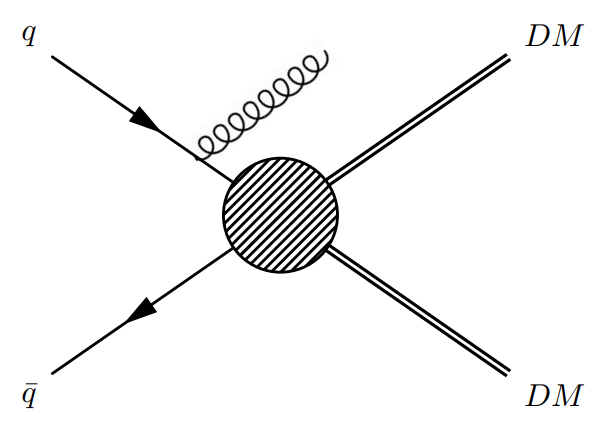
\includegraphics[width=5.5cm, height=4cm]{figs/EFT.png}
\caption{Schematic representation of a typical \ac{EFT} modelization of an \ac{LHC} event with an \ac{ISR} object used to trigger the event \cite{ColliderSearches}.}
\label{fig:EFT}
\end{center}
\end{figure}

\end{itemize}

An additional categorization of the \ac{DM} production models can be done, by separating the so-called s-channel and t-channel models, as shown in Figure~\ref{fig:STChannels}. In the first case, the most common one in collider searches, the mediator between the \ac{SM} and \ac{DM} is assumed to be a boson, and usually decays directly into a pair of \ac{DM} particles. On the other hand, in the t-channel models, the mediator couples to one quark and one \ac{DM} particle, with a colored exchange particle required.

\begin{figure}[htbp]
\begin{center}
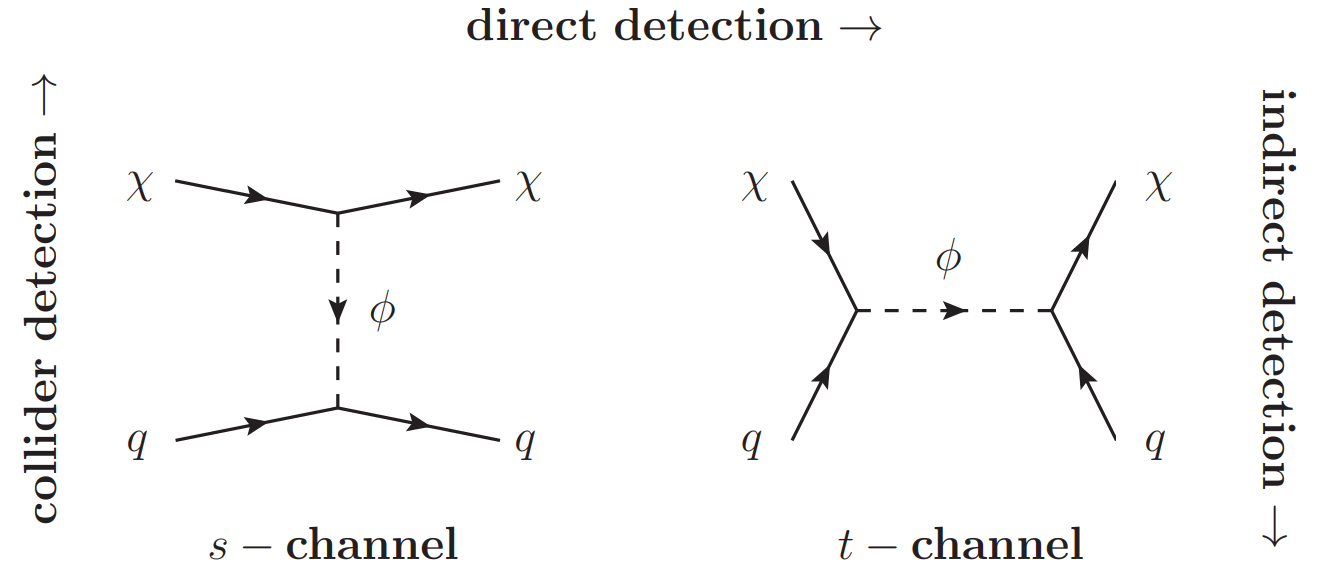
\includegraphics[width=9cm, height=4cm]{figs/STChannels.png}
\caption{Schematic representation of a typical collider \ac{DM} production through s-channel and t-channel processes \cite{STChannels}.}
\label{fig:STChannels}
\end{center}
\end{figure}

In this work, simplified models with either scalar or pseudoscalar mediators will always be considered because of their relative simplicity and the lack of strong assumptions behind them.% We will now study in particular the production and the search for \ac{DM} within the \ac{LHC}.

\section{Dark matter production at the LHC} \label{section:ourChannel}

The \ac{LHC}, colliding protons at a center of mass energy of 13 TeV, is actually a perfect machine to study such processes, because of the expected range of masses (100 GeV to 1 TeV) for the best \ac{DM} candidates, as discussed in Section~\ref{section:DMProperties}. However, because of the weak interactions of such particles, they are not expected to interact at all with the detector, which will then basically search for missing transverse energy along with a \ac{SM} particle triggering the event.

Several major categories of \ac{DM} searches exist at the \ac{LHC}, performed mainly by the \ac{CMS} and \ac{ATLAS} collaborations, depending on the strategy applied for such searches:

\begin{itemize}
\item First of all are the so-called \textbf{mono-X searches}, where X stands for a detectable \ac{SM} particle used to trigger the event while the \ac{DM} mediator usually decays into a pair of particles escaping the detector, leaving behind some \ac{MET}, a key variable to all these searches that will be described in Section~\ref{section:RecoMET}. Depending on the nature of the X particle, several searches can be performed: we can for example mention the mono-$\gamma$ \cite{MonoGammaAtlas, MonoGammaCMS} or mono-jet \cite{MonoJetCMS, MonoJetCMS2} 13 TeV searches performed by the \ac{ATLAS} and \ac{CMS} collaborations.

%\begin{figure}[htbp]
%\begin{center}
%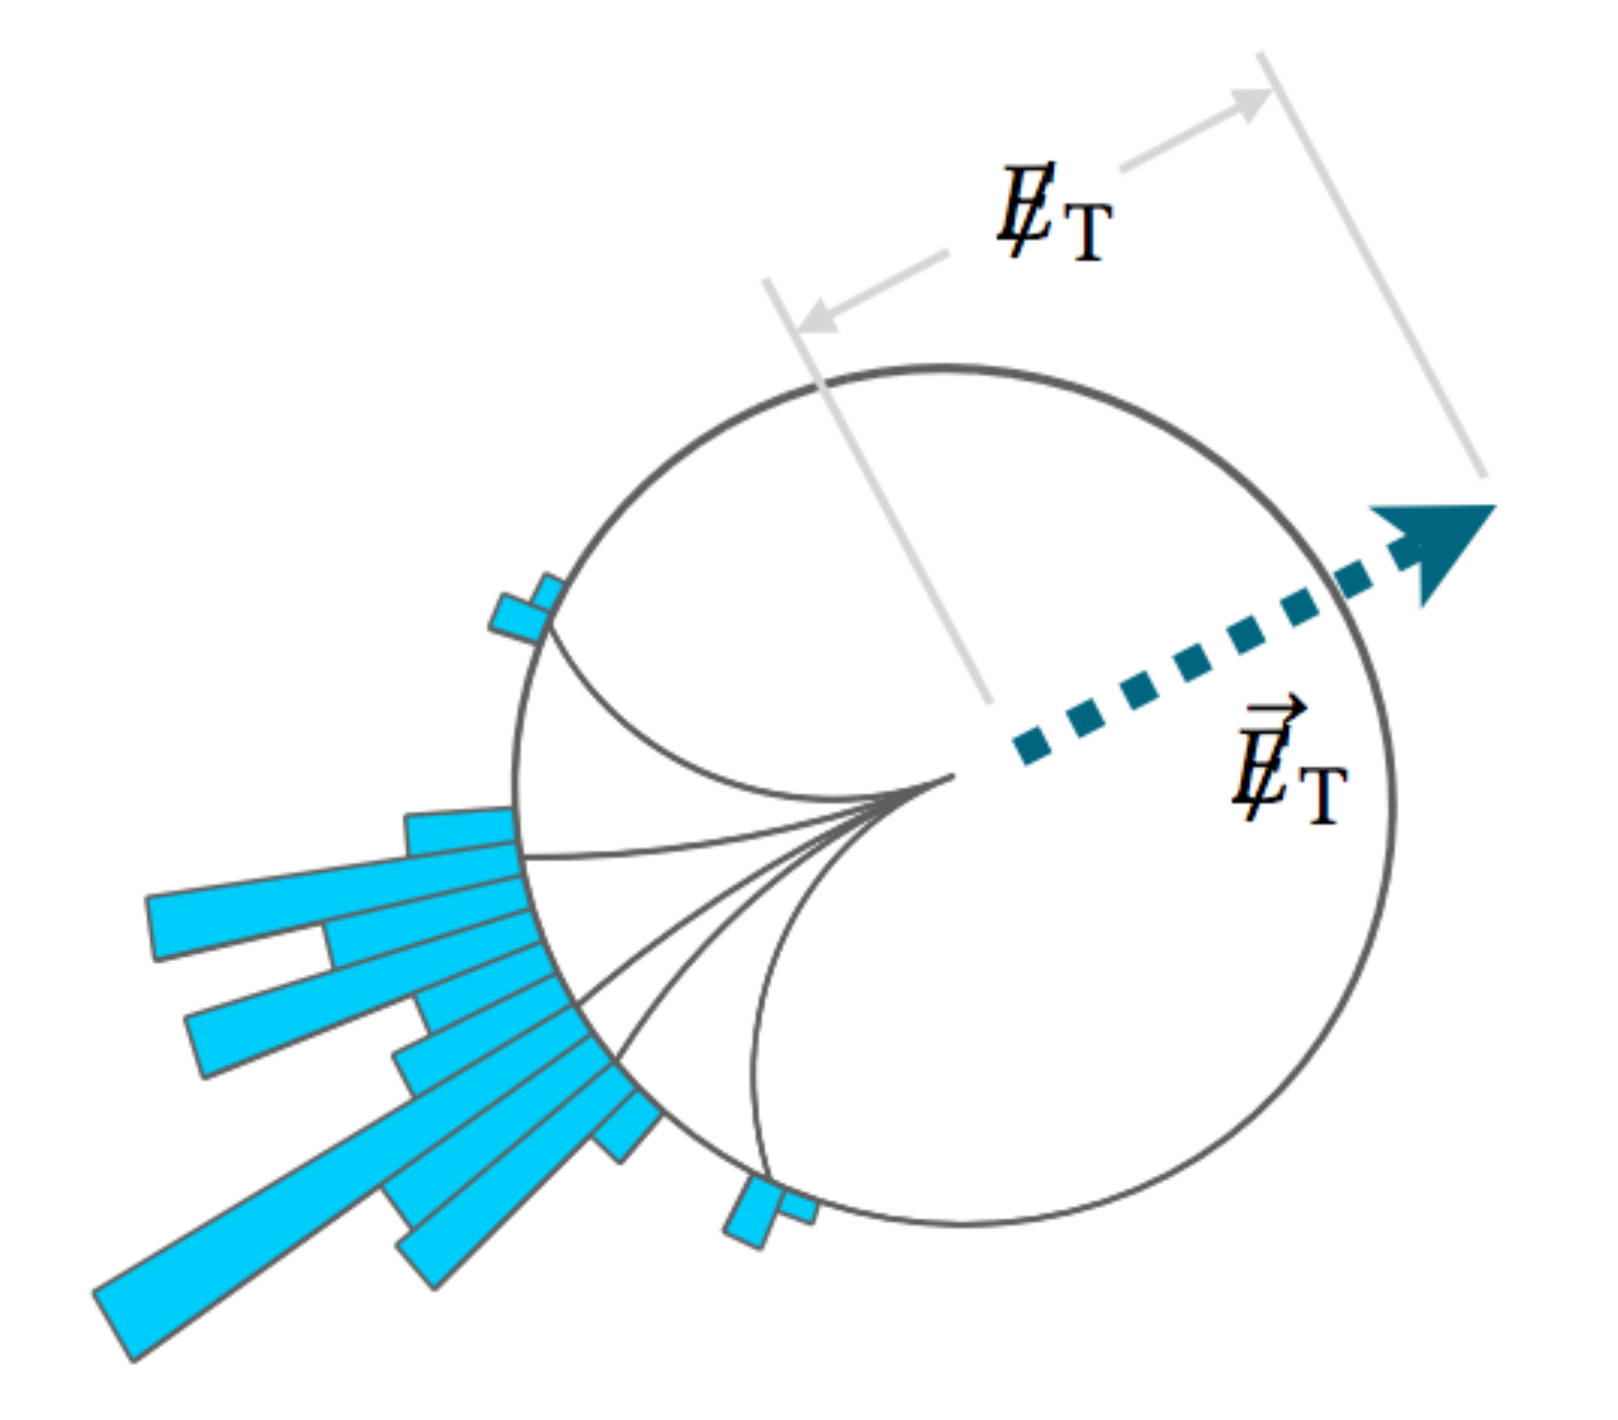
\includegraphics[width=6.5cm, height=5.5cm]{figs/METSchema.png}
%\caption{Schematic representation of a typical mono-X event, with an \ac{ISR} jet in this case going back-to-back with some \ac{MET} \cite{ColliderSearches}.}
%\label{fig:MonoX}
%\end{center}
%\end{figure}

Additionally, if the \ac{DM} mass is high enough, a coupling to the Higgs boson is also possible, or an eventual decay of the Higgs itself to a couple of \ac{DM} particles $H \rightarrow \chi \bar \chi$ is kinematically not impossible. This channel, known as the mono-Higgs, is sensitive to all the decays of the Higgs, even though the searches excluding most of the phase spaces are performed using the $H \rightarrow b \bar b$ and $H \rightarrow \gamma \gamma$ decays \cite{MonoHiggsAtlas, MonoHiggsCMS}. 

\item The searches for \ac{DM} production in \textbf{association with heavy quark(s)} belong to the second category, such as the one performed in this work. Other analyses such as the one probing the $b \bar b$ + DM to its different final states  depending on the decay of the bottom quark (at 8 or 13 TeV) also belong to this group \cite{PreviousDoubleTopAllLep8ATLAS, PreviousDoubleTopBottomAllLep13ATLAS}. 

These searches have to combine the discriminant power of several variables to separate the signal from the backgrounds, since the \ac{MET} distribution on its own is usually not enough, but they present the advantage of being favored by the higher Yukawa coupling to more massive particles implied by the \ac{MFV} assumption.

\item \textbf{Dijet searches} provide the best exclusion limits for most of the spin-1 mediated models considered (up to a few TeV for typical coupling choices) \cite{DijetAtlas, DijetCMS}. In this case, the sensitivity is obtained by searching for either narrow or large resonances on the exponentially falling QCD background, while the other searches were mostly dedicated in searching for bumps in the \ac{MET} spectrum.
\item \textbf{Supersymmetric searches} can also be performed to search for \ac{DM} which would solve the hierarchy problem while giving us perfect \ac{DM} candidates such as the neutralino $\chi$, the lightest stable supersymmetric particle, obtained in many of the \ac{MSSM} theories, having an hypothetical mass below the TeV scale \cite{SUSYDM}.
\item The \textbf{Higgs portal} to the dark sector is another interesting strategy. In some specific cases, when considering spin-0 mediated interactions between the dark and baryonic sectors, the Higgs could be considered as the mediator of the interaction as well, which only requires a minimal modification of the \ac{SM} Lagrangian. It is then necessary to study the different Higgs production modes, such as the gluon fusion and \ac{VBF} mechanisms, to search for an eventual invisible decay of the Higgs into a couple of \ac{DM} particles, assuming that its mass is lower than $\sim 62.5$ GeV, $m_H/2$ \cite{InvisibleHiggs}.
\item Finally, and this is quite new, \textbf{long-lived searches} can also be performed. These are interesting because they can extend the current searches performed to also consider the eventual creation of long-lived particles which would decay a few centimeters further than the primary vertex of the $pp$ collision \cite{LLSearches}. Typical \ac{SM} signatures do not usually include such events, making this channel relatively background-free, even though the reconstruction of the different objects is much harder in this case.
\end{itemize}

All the results from the different searches performed by the \ac{CMS} collaboration using the full ($35.9 \pm 0.9$) fb$^{-1}$ dataset collected at $13$ TeV can be summarized in Figure~\ref{fig:SummarySpin0} for spin-0 mediators and in Figure~\ref{fig:SummarySpin1} when considering spin-1 mediators.

\begin{figure}[htbp]
\centering
\begin{minipage}[b]{.47\textwidth}
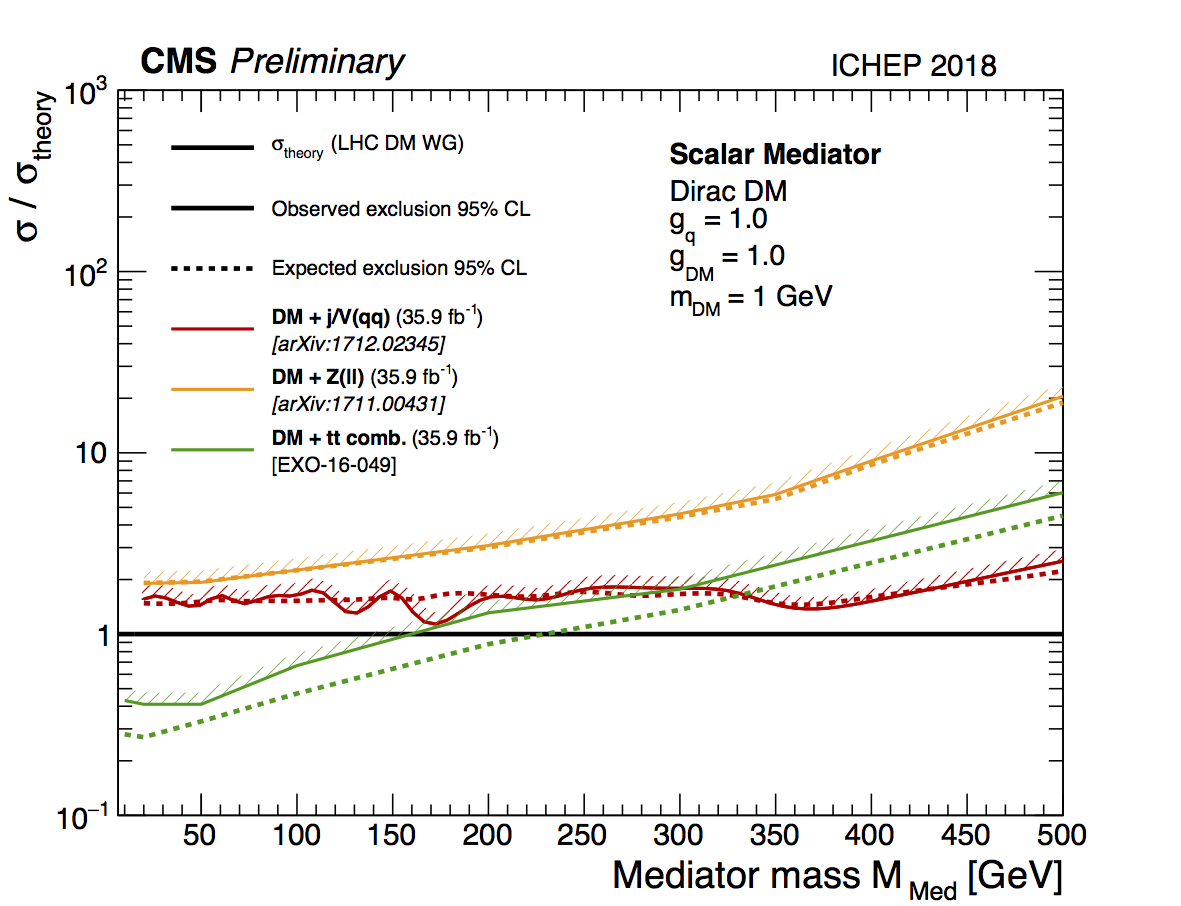
\includegraphics[width=8cm, height=7cm]{figs/SummaryScalar.png}
\end{minipage}\hfill
\begin{minipage}[b]{.47\textwidth}
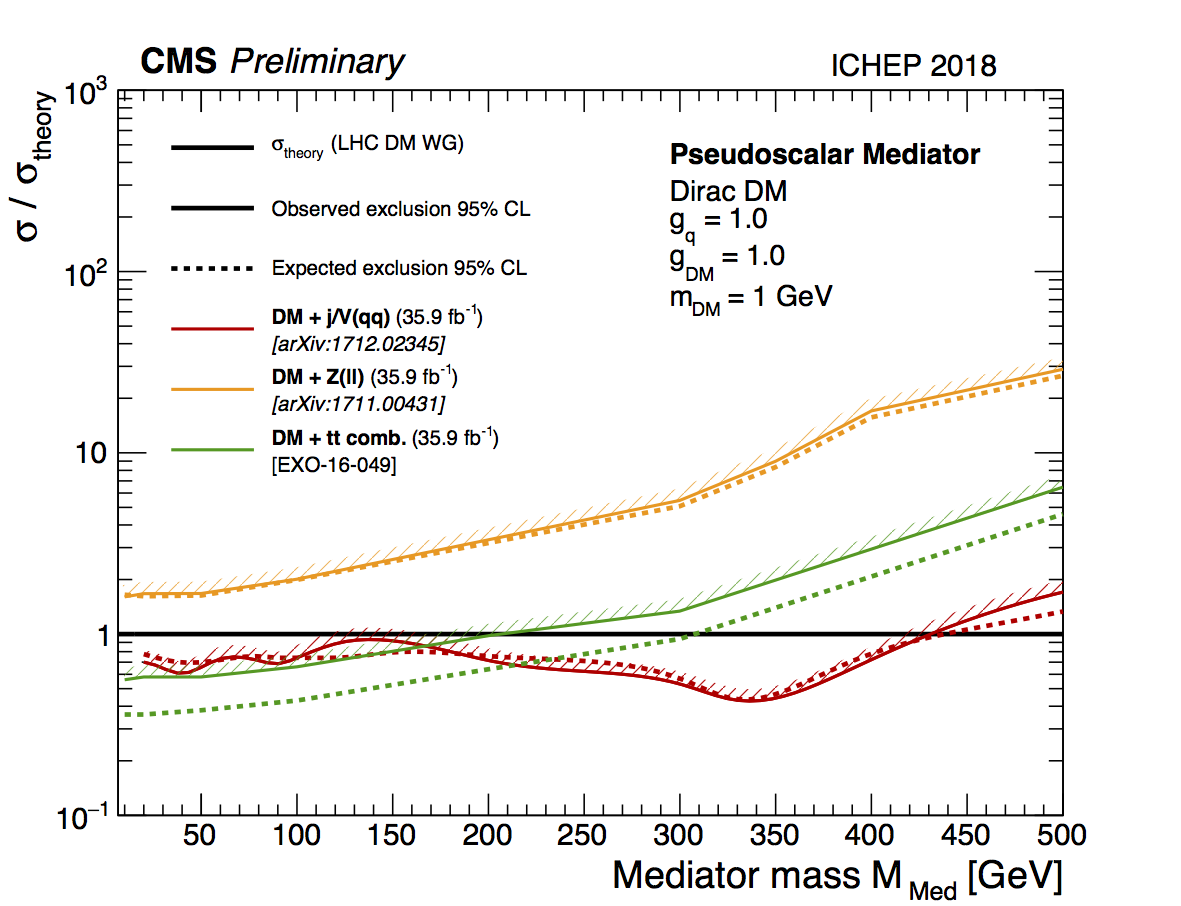
\includegraphics[width=8cm, height=7cm]{figs/SummaryPseudoScalar.png}
\end{minipage} \hfill
\caption{Observed and expected 95\% exclusion limits obtained by different searches of the \ac{CMS} collaboration as a function the spin-0 scalar (on the left) or pseudoscalar (on the right) mediator.}
\label{fig:SummarySpin0}
\end{figure}

\begin{figure}[htbp]
\centering
\begin{minipage}[b]{.47\textwidth}
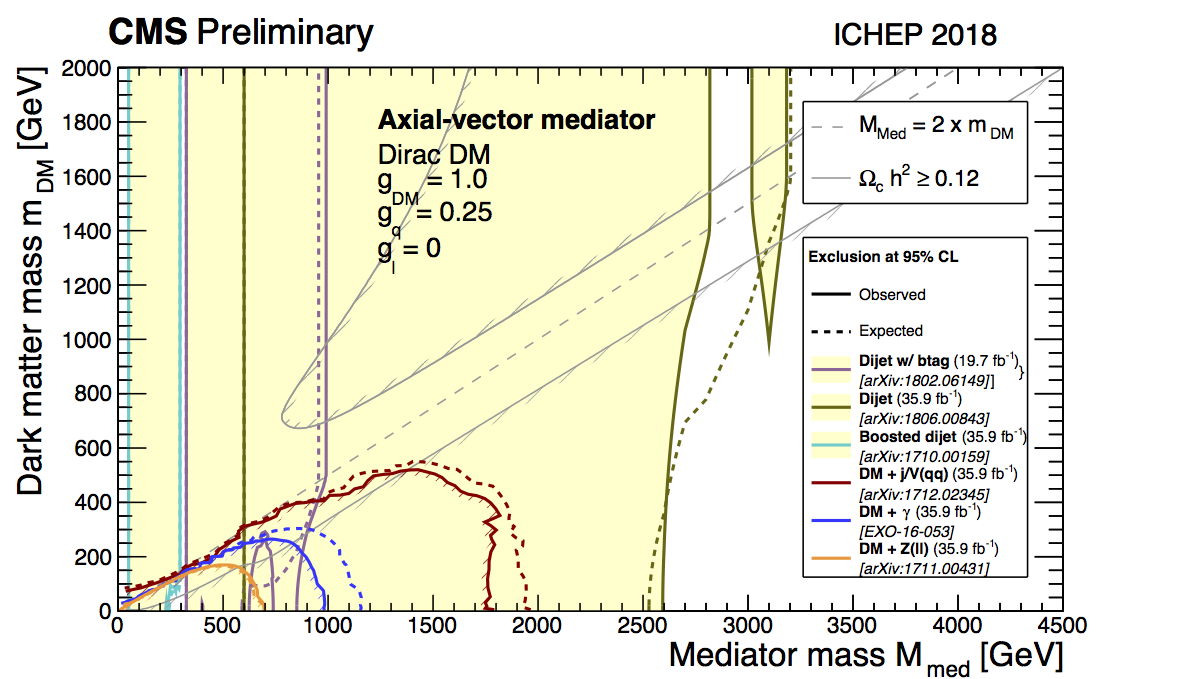
\includegraphics[width=8.5cm, height=5.5cm]{figs/SummaryAxialVector.png}
\end{minipage}\hfill
\begin{minipage}[b]{.47\textwidth}
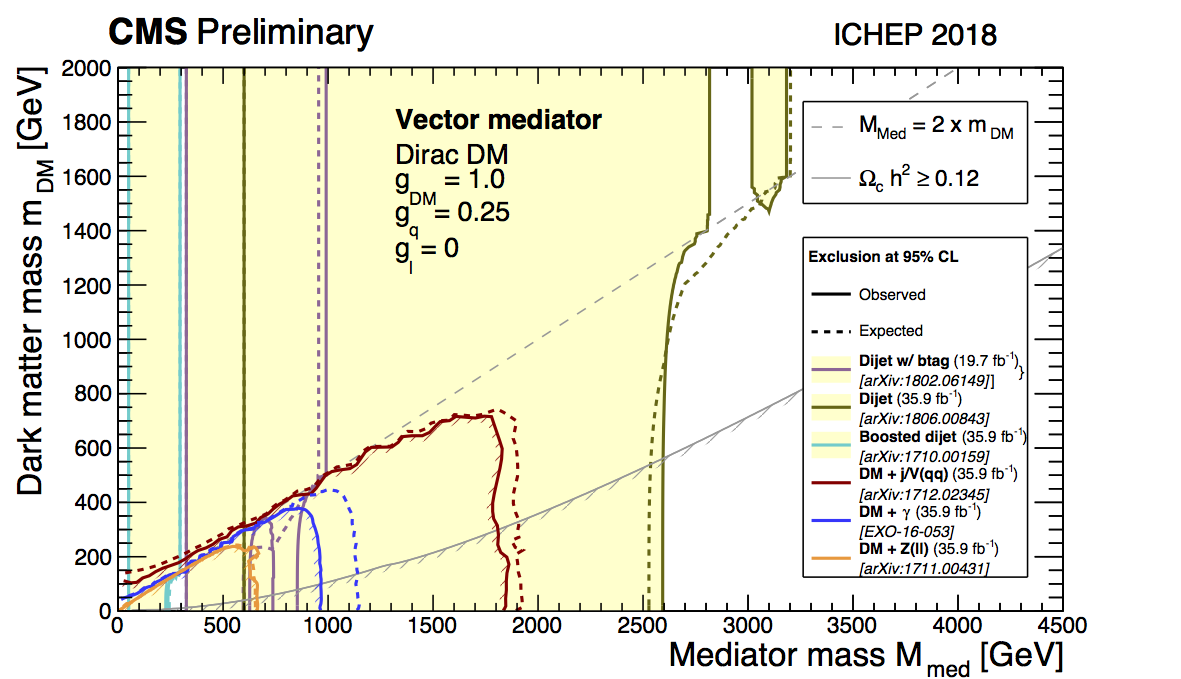
\includegraphics[width=8.5cm, height=5.5cm]{figs/SummaryVector.png}
\end{minipage} \hfill
\caption{Observed and expected 95\% exclusion limits obtained by different searches of the \ac{CMS} collaboration as a function of the spin-1 mediator, considering axial-vector (on the left) and axial (on the right) interactions.}
\label{fig:SummarySpin1}
\end{figure}

These results have also been compared to the results obtained by several direct detection experiments in Figure~\ref{fig:DDComparison}, considering both the \acf{SD} and \acf{SI} cases, as explained in Section~\ref{subsection:DirectSearches}.

\begin{figure}[htbp]
\centering
\begin{minipage}[b]{.47\textwidth}
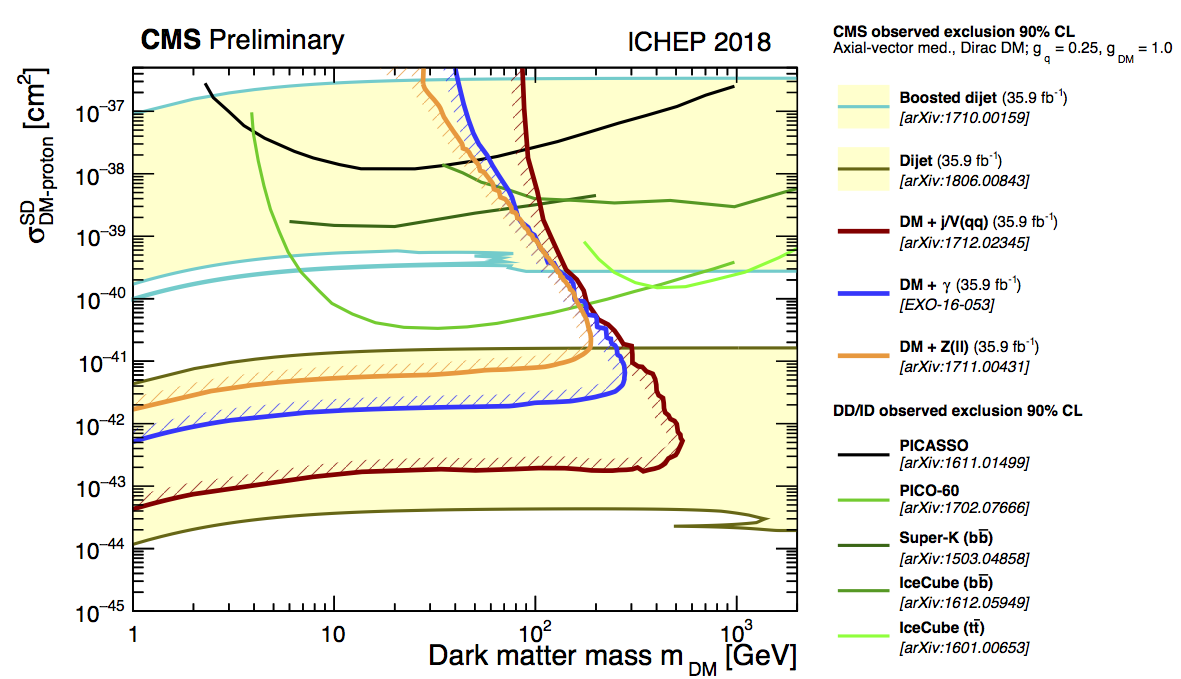
\includegraphics[width=8.5cm, height=5.4cm]{figs/SDDD.png}
\end{minipage}\hfill
\begin{minipage}[b]{.47\textwidth}
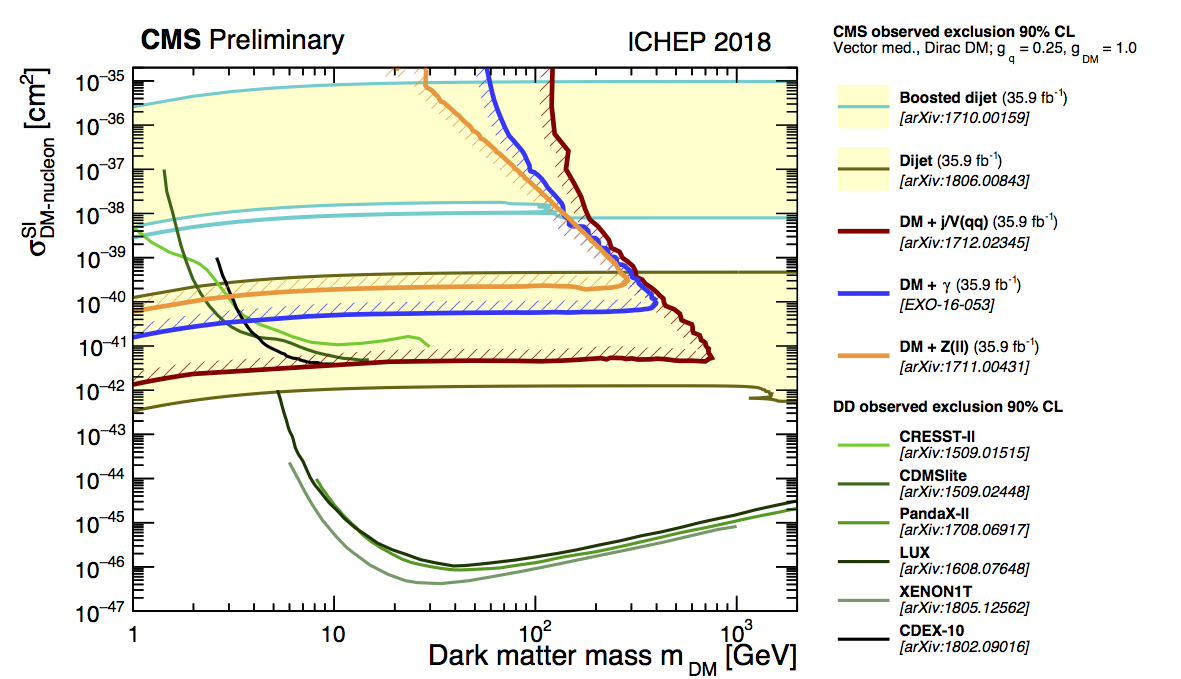
\includegraphics[width=8.5cm, height=5.4cm]{figs/SIDD.png}
\end{minipage} \hfill
\caption{\ac{CMS} 90\% exclusion limits compared to the most famous direct detection experiments for the \ac{SD} (on the left) and \ac{SI} (on the right) scenarios, obtained using similar couplings.}
\label{fig:DDComparison}
\end{figure}

This particular analysis and our signal of interest, the search for \ac{DM} production together with a single or a pair of top quarks falls into the second category. It is already important to note that this analysis has been performed considering the \ac{DM} candidate to be a Dirac fermion with all the couplings equal and set to 1, as recommended by the \ac{DMWG} \cite{DMWG}.

\subsection{The single top production channel} \label{subsection:singleTopChannel}

The first kind of signal considered in this analysis is the production of \ac{DM} in association with a single top quark, known as $t/\bar t$+DM analysis. This process is expected to be mediated by a spin-0 mediator, either scalar or pseudoscalar, and is associated with a light quark and a W boson (the mono-top analysis is dealing with the case where a single top is created without any additional particle). 

Three different Feynman diagrams can be associated to this particular analysis depending on the model considered, as shown in Figure~\ref{fig:singleTopFeynman}.

%\begin{figure}[htbp]
%\centering
%\begin{minipage}[b]{.3\textwidth}
%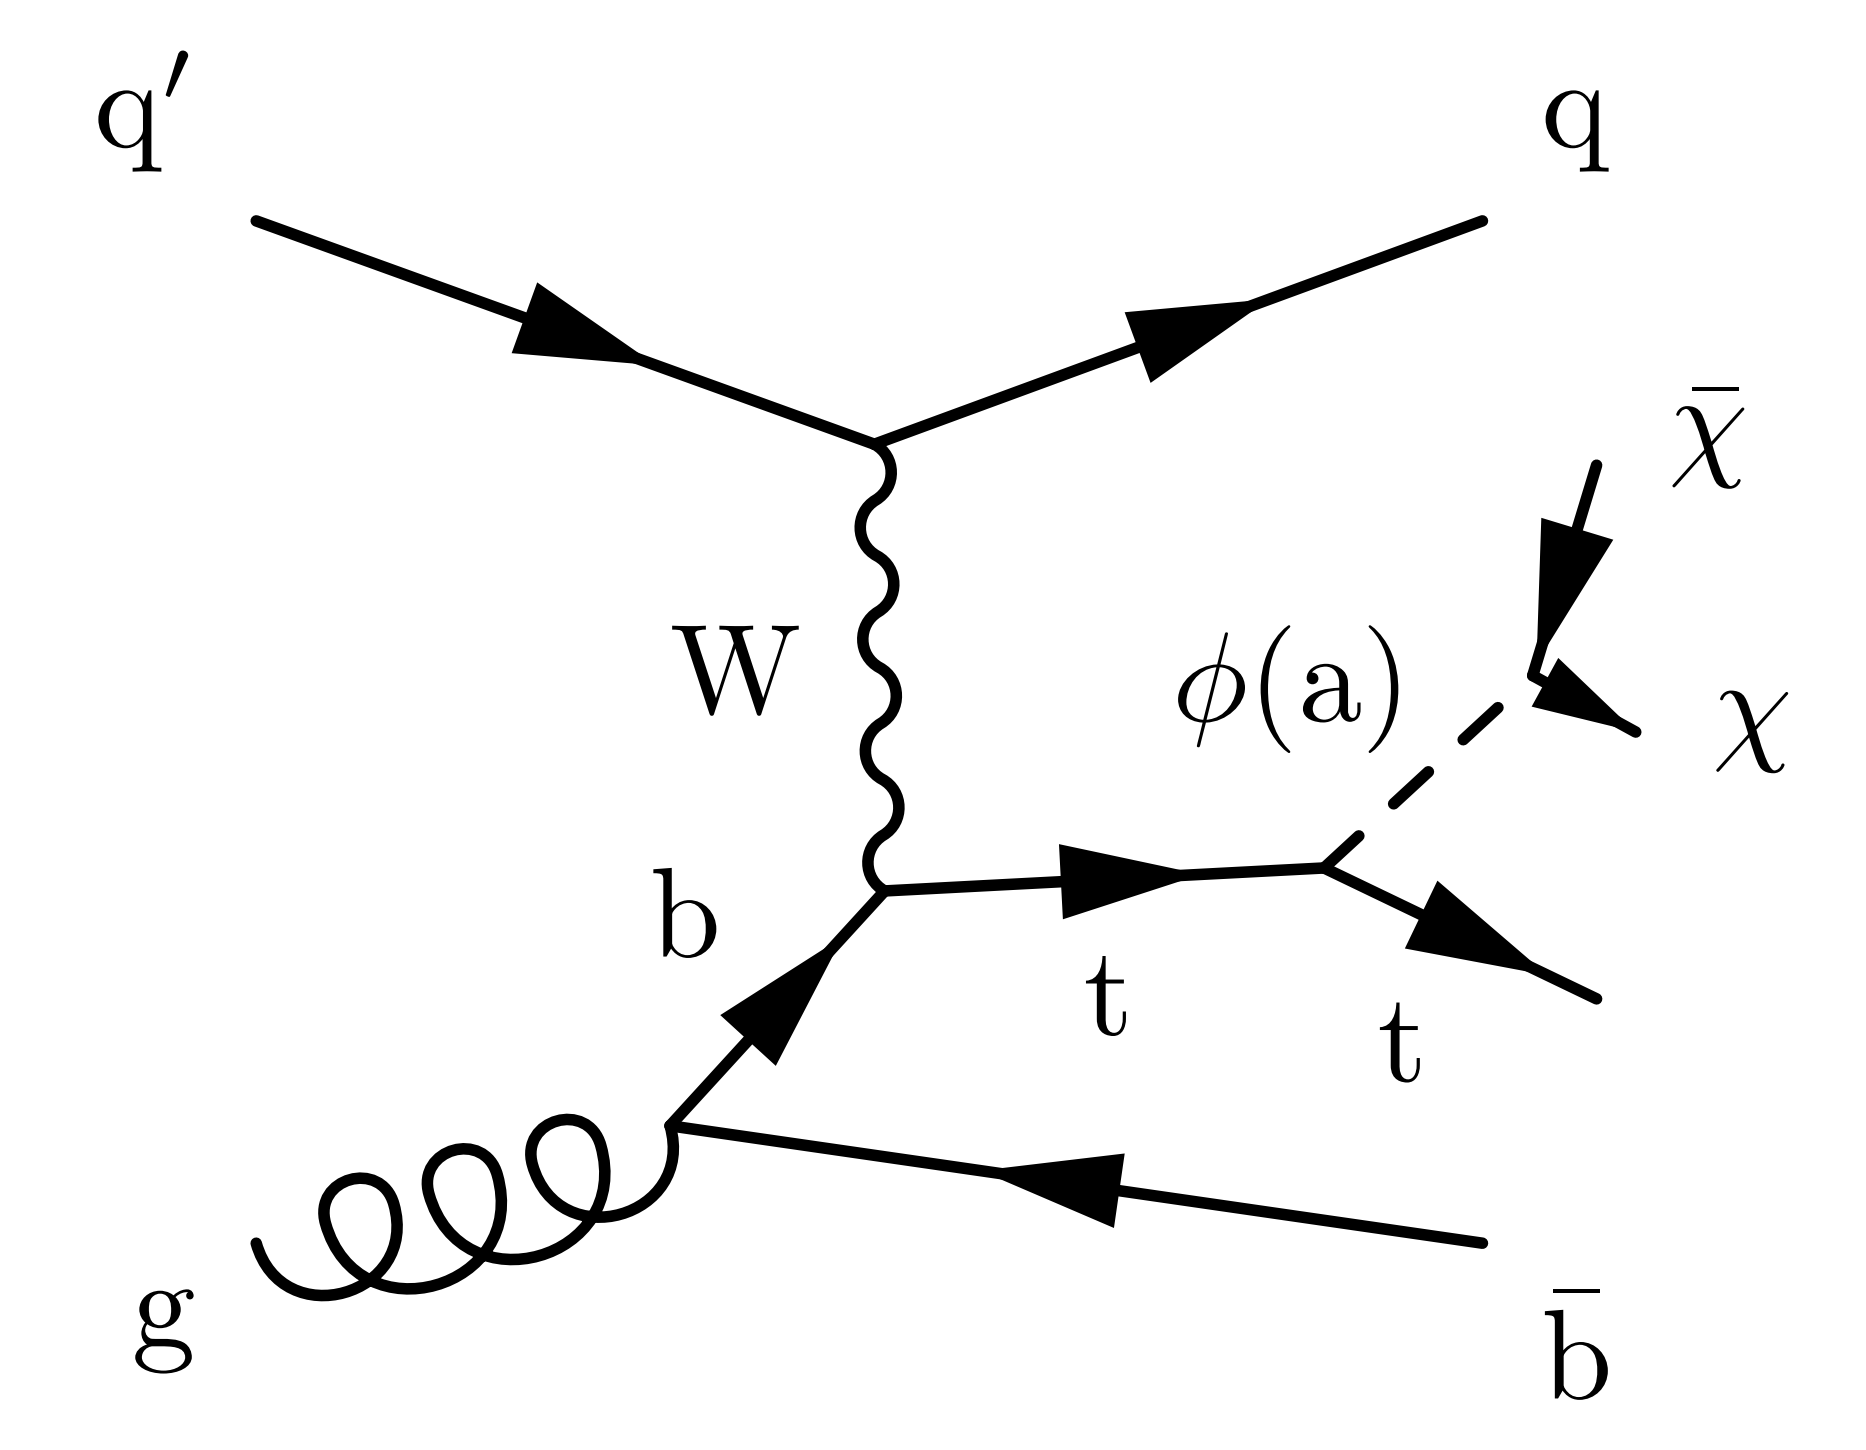
\includegraphics[width=4.8cm, height=3.5cm]{figs/tDMa.png}
%\end{minipage}\qquad
%\begin{minipage}[b]{.3\textwidth}
%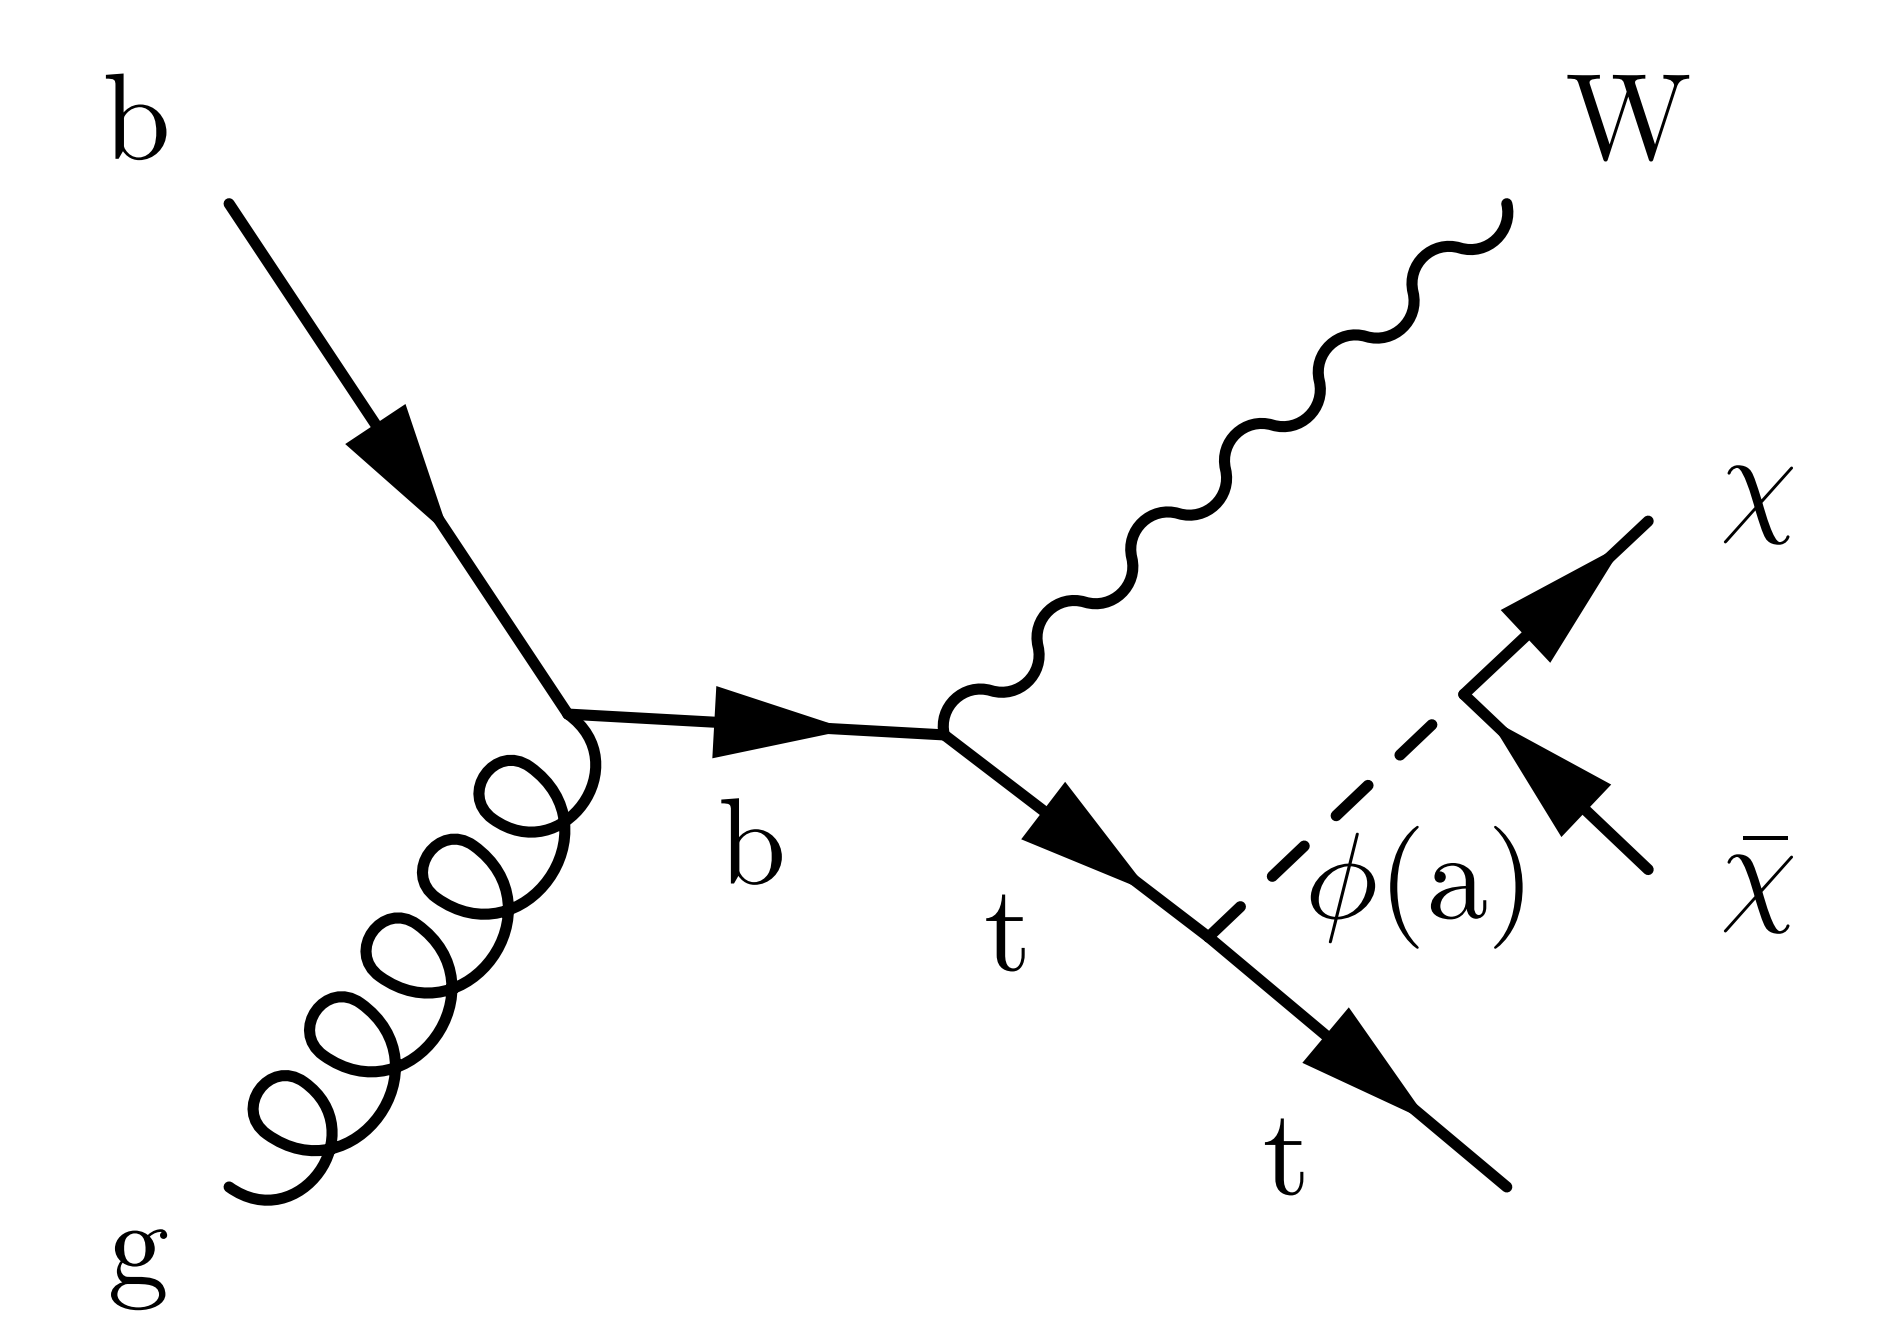
\includegraphics[width=4.8cm, height=3.5cm]{figs/tDMb.png}
%\end{minipage}
%\begin{minipage}[b]{.28\textwidth}
%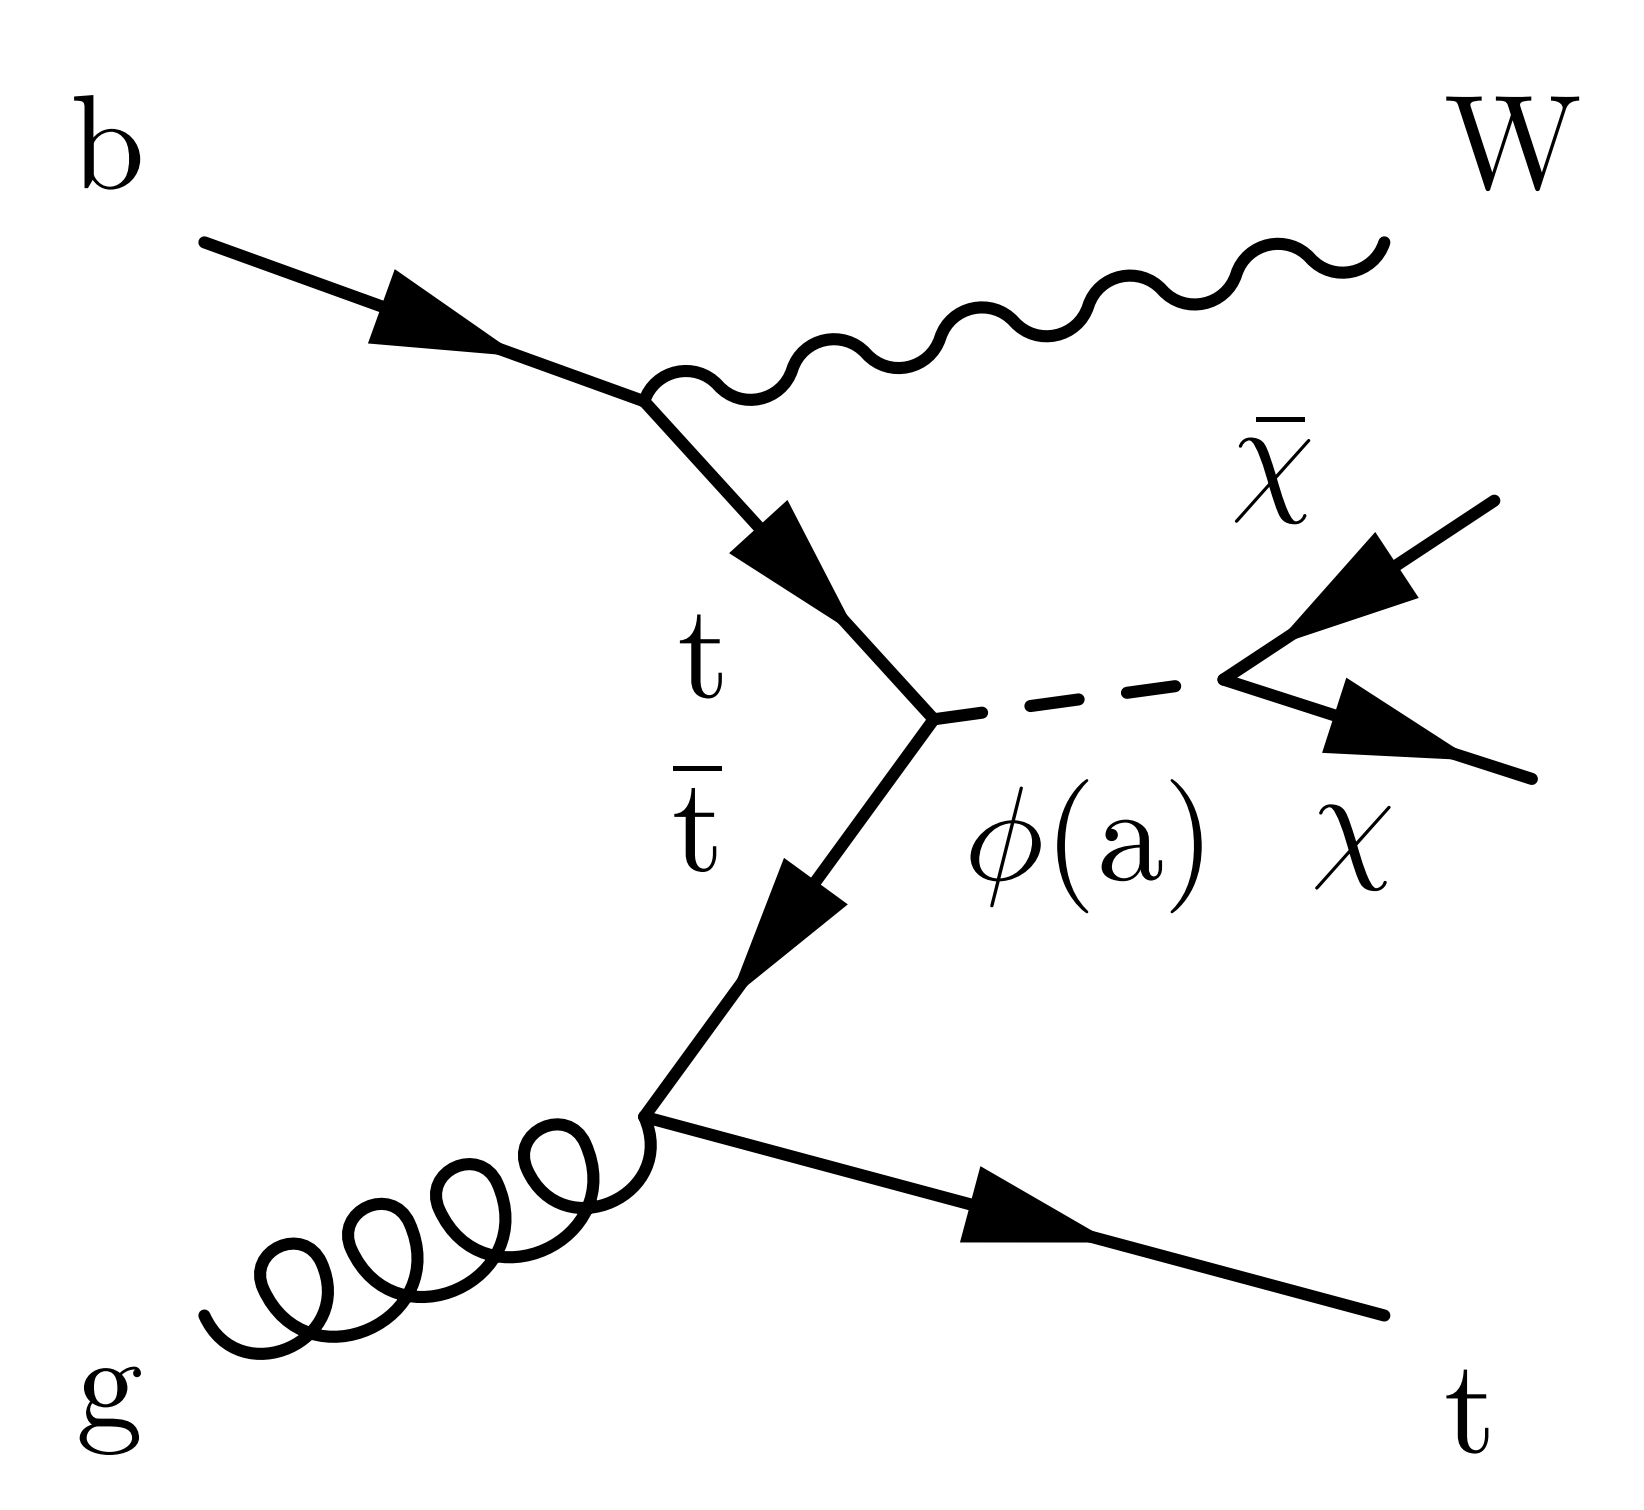
\includegraphics[width=4.8cm, height=3.5cm]{figs/tDMc.png}
%\end{minipage}
%\caption{Feynman diagrams involving the production of \ac{DM} with a single top quark with its associated t-channel W boson (on the left), or tW (on the center and on the right) production.}
%\label{fig:singleTopFeynman}
%\end{figure}

\begin{figure}[htbp]
\centering
\begin{minipage}{.31\textwidth}
\resizebox{\textwidth}{!}{
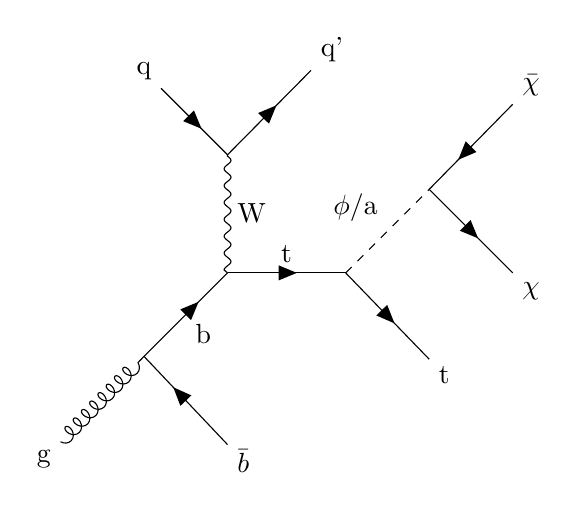
\begin{tikzpicture}
  \begin{feynman}  
    \vertex (qi) {q};
    \vertex (a) [below right=of qi];
	\vertex (qf) [above right=of a] {q'};
	\vertex (b) [below=of a];
	\vertex (b1);     
    \vertex (c) [below left=of b];
    \vertex (gi) [below left=of c] {g};
    \vertex (bf) [below right=of c] {$\bar b$};
    \vertex (d) [right=of b];
    \vertex (t1);
    \vertex (e) [above right=of d];
    \vertex (tf) [below right=of d] {t};
    \vertex (d1) [above right=of e] {$\bar \chi$};
    \vertex (d2) [below right=of e] {$\chi$};
        
    \diagram* {
      (qi) -- [fermion] (a) -- [fermion] (qf),
      (a) -- [boson, edge label={W}] (b),
      (b) -- [anti fermion, edge label={b}] (c),
      (gi) -- [gluon] (c) -- [anti fermion] (bf),
      (b)-- [fermion, edge label={t}] (d),
      (d) -- [scalar, edge label={$\phi$/a}] (e),
      (d) -- [fermion] (tf),
      (e) -- [fermion] (d2),
      (e) -- [anti fermion] (d1)
    };
  \end{feynman}
\end{tikzpicture}
}
\end{minipage} \hfill
\begin{minipage}{.31\textwidth}
\resizebox{\textwidth}{!}{
\begin{tikzpicture}
  \begin{feynman}  
    \vertex (bi) {b};
    \vertex (a) [below right=of qi];
	\vertex (gi) [below left=of a] {g};
	\vertex (b) [right=of a];
	\vertex (W) [above right=of b];     
    \vertex (c) [below right=of b];
    \vertex (d) [above right=of c];
    \vertex (tf) [below right=of c] {t};
    \vertex (d1) [above right=of d] {$\bar \chi$};
    \vertex (d2) [below right=of d] {$\chi$};
        
    \diagram* {
      (bi) -- [fermion] (a) -- [fermion, edge label={b}] (b),
      (gi) -- [gluon] (a),
      (b) -- [boson, edge label={W}] (W),
      (b) -- [fermion, edge label={}] (c),
      (c) -- [scalar, edge label={$\phi$/a}] (d),
      (d) -- [fermion] (d2),
      (d) -- [anti fermion] (d1),
      (c) -- [fermion] (tf)
    };
  \end{feynman}
\end{tikzpicture}
}
\end{minipage} \hfill
\begin{minipage}{.31\textwidth}
\resizebox{\textwidth}{!}{
\begin{tikzpicture}
  \begin{feynman}  
    \vertex (bi) {b};
    \vertex (a) [below right=of qi];
    \vertex (W) [above right=of a] {W};
    \vertex (b) [below right=of a];
    \vertex (c) [below left=of b];
	\vertex (gi) [below left=of c] {g};
	\vertex (tf) [below right=of c] {t};
	\vertex (d) [right=of b];
	\vertex (d1) [above right=of d] {$\bar \chi$};
    \vertex (d2) [below right=of d] {$\chi$};
        
    \diagram* {
      (bi) -- [fermion] (a) -- [boson] (W),
      (a) -- [fermion, edge label={t}] (b),
      (b) -- [fermion, edge label={$\bar t$}] (c),
		(gi) -- [gluon] (c),
		(c) -- [fermion] (tf)    ,
		(b) -- [scalar, edge label={$\phi$/a}] (d),
      (d) -- [fermion] (d2),
      (d) -- [anti fermion] (d1)  
    };
  \end{feynman}
\end{tikzpicture}
}
\end{minipage} \hfill
\caption{Feynman diagrams involving the production of \ac{DM} with a single top quark according to its t-channel W boson (on the left), or tW (on the center and on the right) production modes.}
\label{fig:singleTopFeynman}
\end{figure}

As discussed previously, the top quark will be dynamically favored due to its high mass and therefore high Yukawa coupling, but this has another consequence as well, since the lifetime of this quark is extremely low, of the order of $10^{-15}$ s \cite{PDG}. This means that this particle usually decays before being able to form hadrons, so we can only detect the products of its decay, not the top quark itself. In almost 100\% of the cases, the top actually decays into a bottom quark and a W boson, which decays itself before being detected into quarks and/or leptons. Even though this will be detailed in Chapter~\ref{chapter:Selection}, we can already conclude that the typical final state of such signature is therefore made out of \ac{MET} coming from the \ac{DM}, one b-tagged jet along with one or two W bosons, seen as a combination of jets and leptons, depending on the channel considered.

\subsection{The $t \bar t$ production channel} \label{subsection:ttChannel}

The $t \bar t$+DM analysis is really similar, except that in this case, we have two top quarks in the final state, as represented in Figure~\ref{fig:ttDMFeynman}.

%\begin{figure}[htbp]
%\begin{center}
%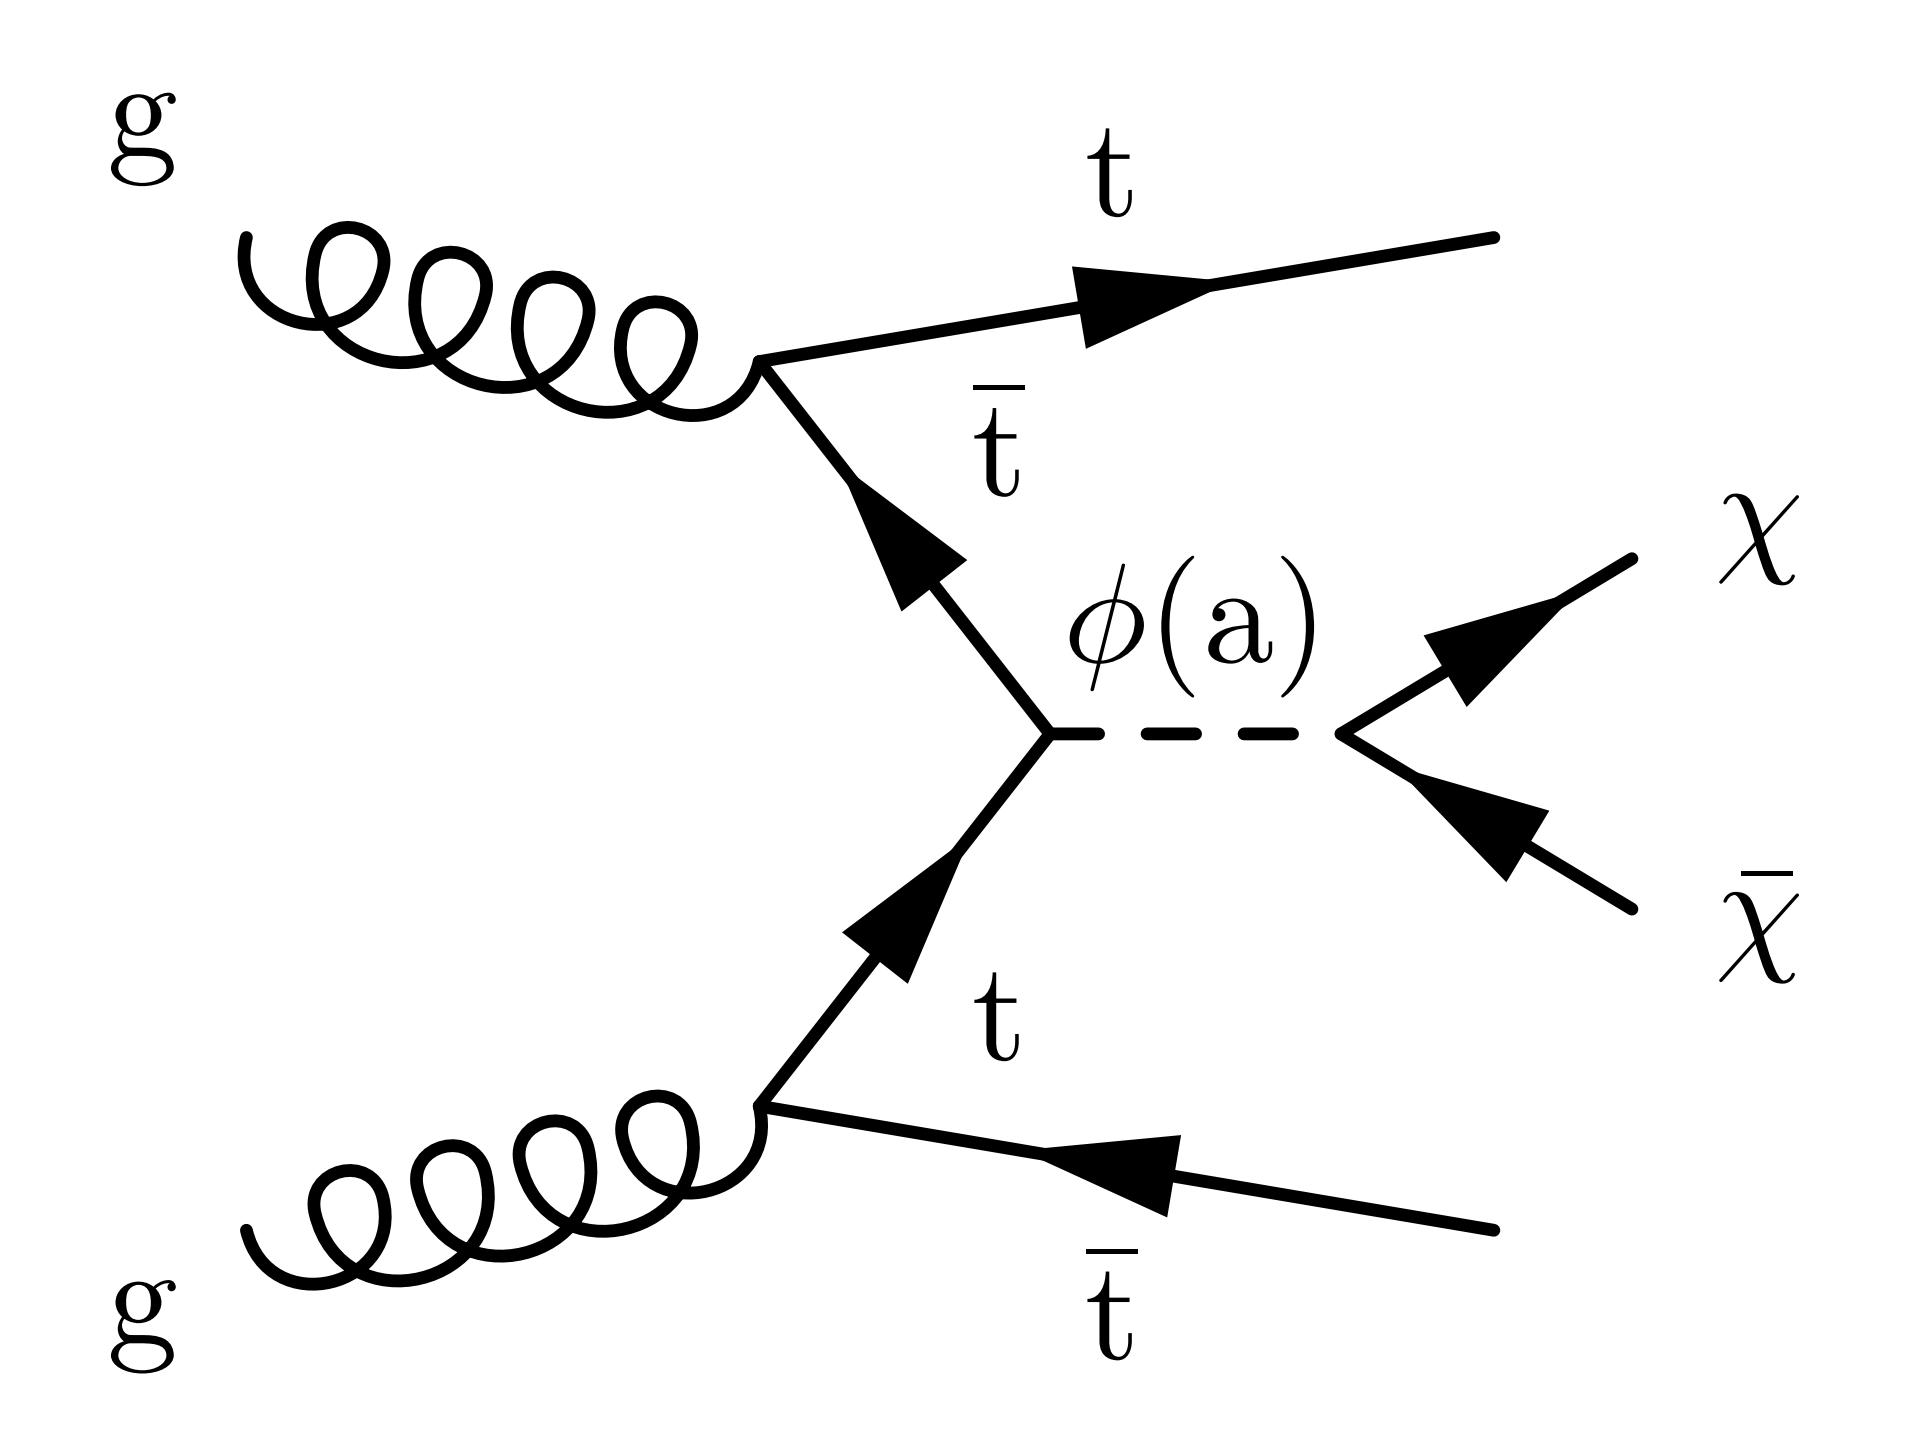
\includegraphics[width=4.5cm, height=3.5cm]{figs/ttDM.png}
%\caption{Schematic representation of a typical $t \bar t$+DM event.}
%\label{fig:ttDMFeynman}
%\end{center}
%\end{figure}

\begin{figure}[htbp]
\begin{center}
\resizebox{0.35\textwidth}{!}{
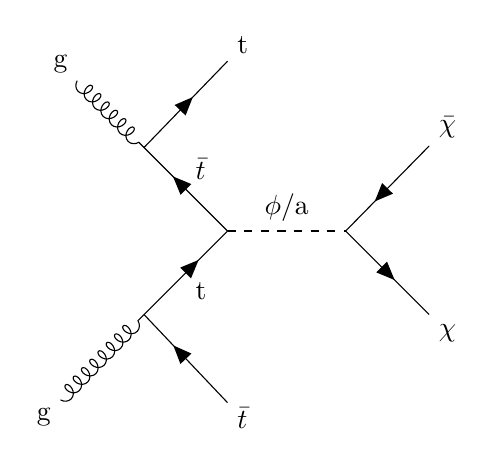
\begin{tikzpicture}
  \begin{feynman}  
    \vertex (gi1) {g};
    \vertex (a) [below right=of gi1];
    \vertex (tf1) [above right=of a] {t};
    \vertex (b) [below right=of a];
    \vertex (c) [below left=of b];
	\vertex (gi2) [below left=of c] {g};
	\vertex (tf2) [below right=of c] {$\bar t$};
	\vertex (d) [right=of b];
	\vertex (d1) [above right=of d] {$\bar \chi$};
    \vertex (d2) [below right=of d] {$\chi$};
        
    \diagram* {
      (gi1) -- [gluon] (a) -- [fermion] (tf1),
      (a) -- [anti fermion, edge label={$\bar t$}] (b),
      (b) -- [anti fermion, edge label={t}] (c),
		(gi2) -- [gluon] (c) -- [anti fermion] (tf2)    ,
		(b) -- [scalar, edge label={$\phi$/a}] (d),
      (d) -- [fermion] (d2),
      (d) -- [anti fermion] (d1)  
    };
  \end{feynman}
\end{tikzpicture}
}
\caption{Schematic representation of a typical $t \bar t$+DM event.}
\label{fig:ttDMFeynman}
\end{center}
\end{figure}

The final state expected by such an event is therefore made of two b-tagged jets, along with two W bosons and some \ac{MET} coming from the pair of \ac{DM} particles. In this case as well, both scalar $\phi$ and pseudoscalar $a$ mediators will be considered, with a mass range from 10 to 500 GeV.

\subsection{The dilepton final state} \label{subsection:diLeptonFS}

As previously explained, most of the models considered will produce exactly two W bosons, which are not stable long enough and therefore decay before reaching the detector, meaning that we cannot directly detect such bosons. However, we can detect the results of the decays of these W, since they can decay either to hadrons ($67.6 \pm 0.27 \%$ branching ratio) or to a lepton and a neutrino, giving us an additional contribution of \ac{MET} ($10.8 \pm 0.09 \%$ for each lepton) \cite{PDG}.

This means that this kind of analyses featuring two W bosons in the final state can focus on different channels: either completely hadronic (if both the W decay into quarks), semileptonic or dileptonic (when both W bosons decay into two neutrinos and two leptons of opposite charge). 

Given the \ac{BR} of the W decay, it is easy to see that the dileptonic channel, which will be the focus of this work, is not favored statistically. However, this channel features less backgrounds than other channels, resulting in a better signal isolation, and because leptons can usually be reconstructed in a better way than jets (cf. Chapter~\ref{chapter:Reco}), resulting in lower uncertainties and in improved limits.

\section{Previous relevant results} \label{section:PreviousResults}

This analysis being performed at a center of mass energy $\sqrt{s} = 13$ TeV, only the most relevant results to this energy obtained by both the \ac{CMS} and \ac{ATLAS} collaborations will be quoted. 

First of all, the \textbf{\ac{ATLAS} collaboration} published interesting results at this center of mass energy, considering an integrated luminosity of 13.3 fb$^{-1}$, and obtained the corresponding exclusion limits at the 95\% \ac{CL}, considering the $t \bar t$+DM model and both scalar and pseudoscalar spin-0 mediators for the interaction, as shown in Figure~\ref{fig:ATLAS13}. In this case, and for the couplings considered, an exclusion up to $\sim375$ GeV has been achieved \cite{PreviousDoubleTopNoLep13ATLAS}.

\begin{figure}[htbp]
\begin{center}
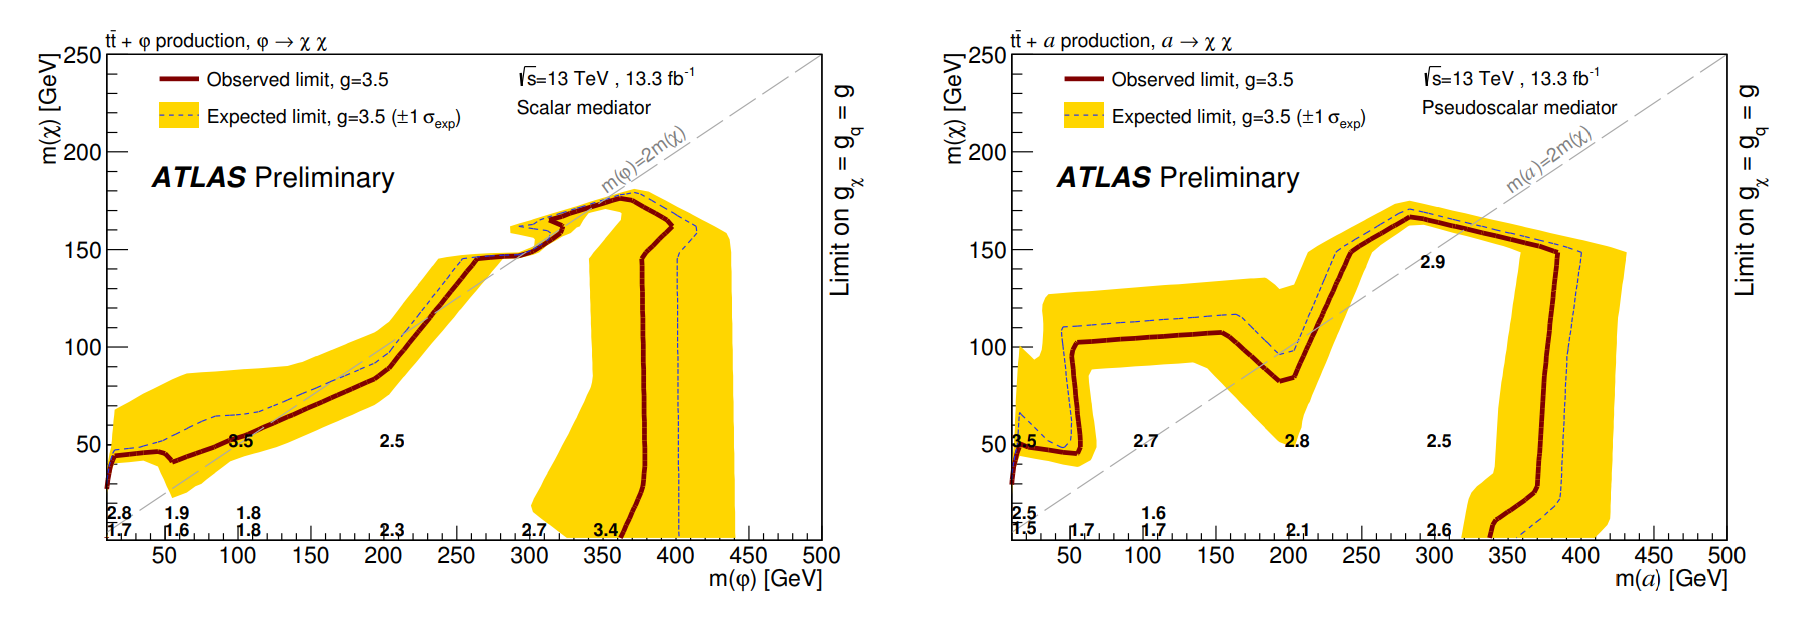
\includegraphics[width=14cm, height=5.8cm]{figs/Atlasttbar13fb.png}
\caption{Limits on the \ac{DM} and mediator masses obtained by \ac{ATLAS} using 13.3 fb$^{-1}$ of 13 TeV data, considering scalar (on the left) and pseudoscalar (on the right) mediators \cite{PreviousDoubleTopNoLep13ATLAS}.}
\label{fig:ATLAS13}
\end{center}
\end{figure}

Considering the full 2016 dataset of $36.1$ fb$^{-1}$, similar results have been obtained, as shown in Figure~\ref{fig:atlas36}. In this case, and for lower coupling values, an exclusion up to around 100 GeV has been obtained considering scalar and pseudoscalar mediators \cite{PreviousDoubleTopBottomAllLep13ATLAS}.

\begin{figure}[htbp]
\centering
\begin{minipage}[b]{.4\textwidth}
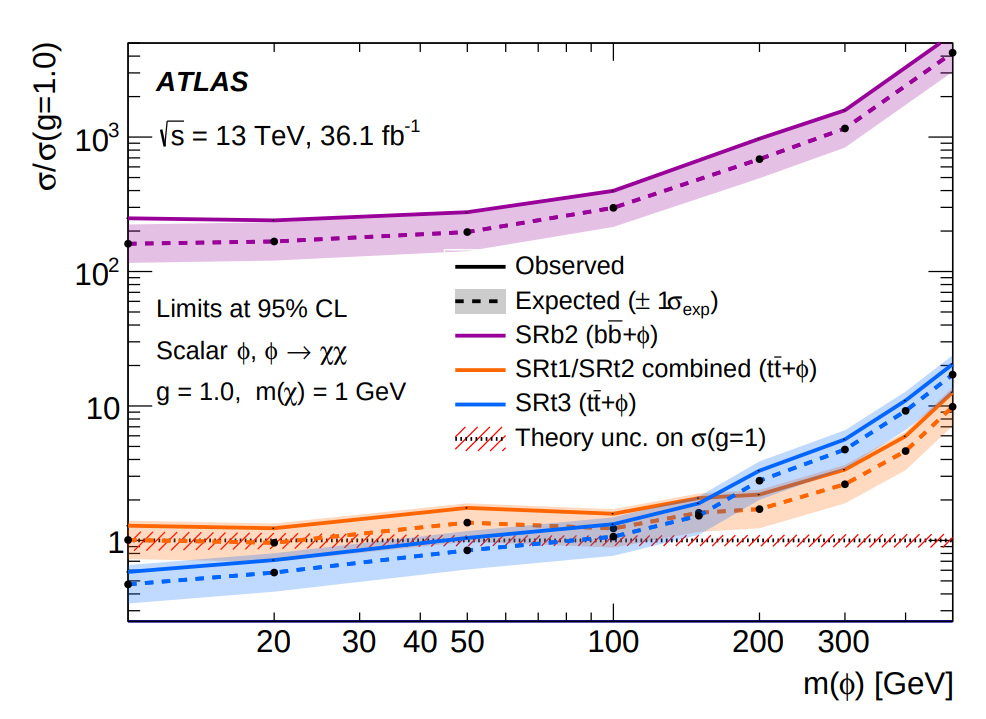
\includegraphics[width=7cm, height=6cm]{figs/Atlas36a.png}
\end{minipage}\hfill
\begin{minipage}[b]{.48\textwidth}
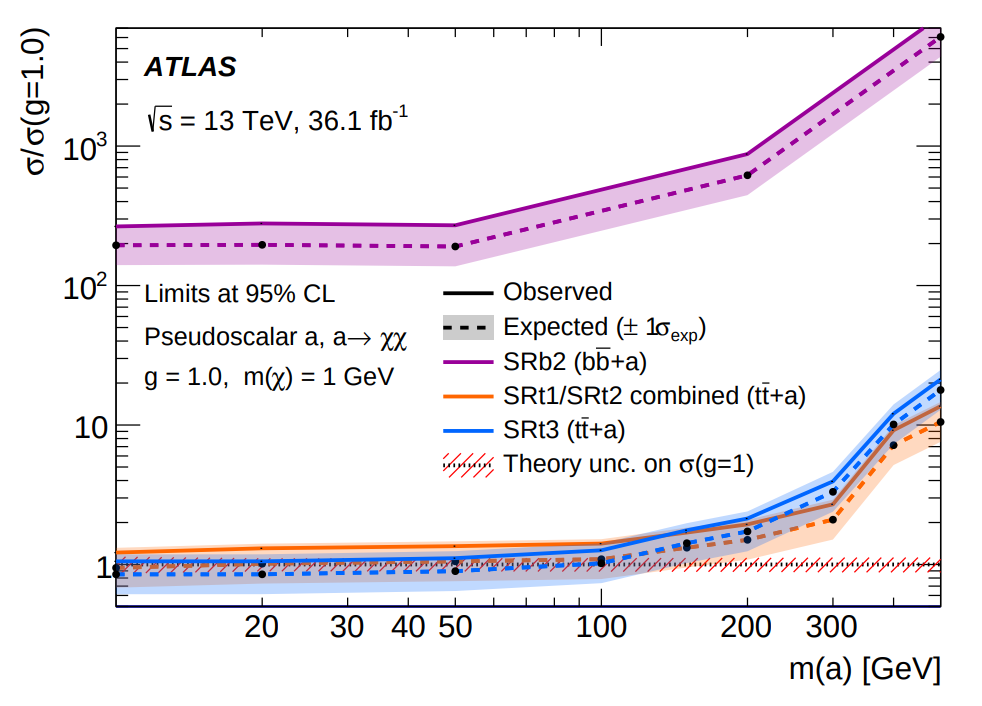
\includegraphics[width=7cm, height=5.88cm]{figs/Atlas36b.png}
\end{minipage}\hfill
\caption{Exclusion limits at the 95\% \ac{CL} obtained by \ac{ATLAS} considering  scalar (on the left) and pseudoscalar (on the right) mediators, for a \ac{DM} mass of 1 GeV \cite{PreviousDoubleTopBottomAllLep13ATLAS}.}\label{fig:atlas36}
\end{figure}

Finally, \ac{ATLAS} recently presented in ICHEP 2020 the first results for a combined search of stop and for a similar final state in the dilepton final state, and using the full Run II dataset, as shown in Figure~\ref{fig:ATLASICHEP} \cite{ATLASICHEP2020}. According to these latest results, the collaboration has now been able to achieve an exclusion of scalar (pseudoscalar) mediators with masses up to 250 (300) GeV.

 \begin{figure}[htbp]
\centering
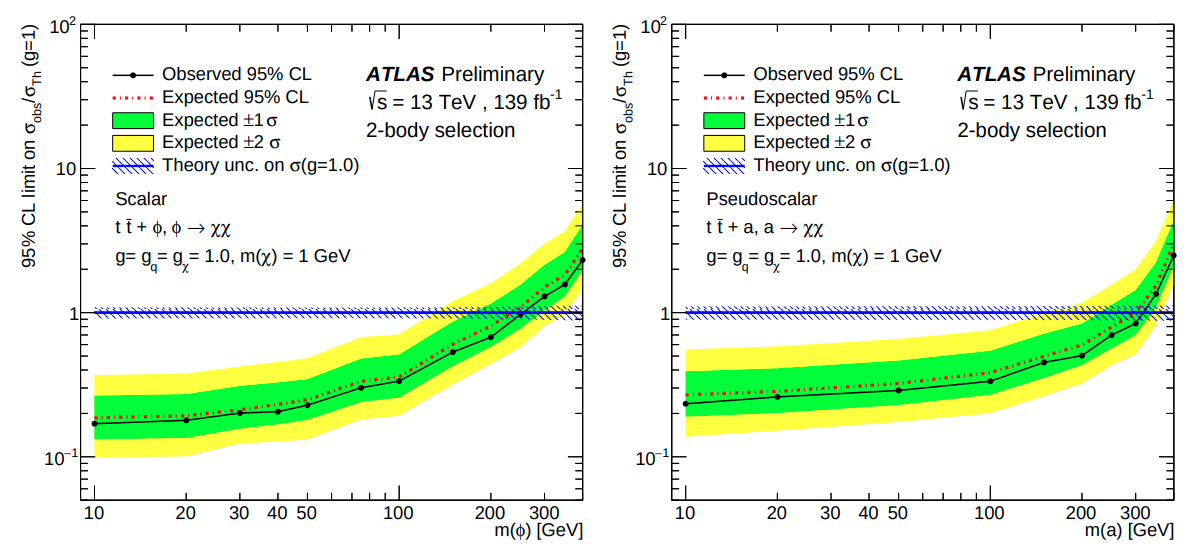
\includegraphics[width=14cm, height=6.3cm]{figs/ATLASICHEP.png}
\caption{Exclusion limits at the 95\% \ac{CL} obtained by \ac{ATLAS} considering  scalar (on the left) and pseudoscalar (on the right) mediators, for a \ac{DM} mass of 1 GeV, considering the dilepton final state of such model and the full Run II dataset \cite{PreviousDoubleTopBottomAllLep13ATLAS}.}\label{fig:ATLASICHEP}
\end{figure}

The \textbf{\ac{CMS} collaboration} published in 2018 a similar analysis, using the $35.9$ fb$^{-1}$ of data collected during the year 2016. This analysis combined the three different final states possible (hadronic, semileptonic and dileptonic) and computed the limits on the signal strength for different mediator and dark matter masses, considering both scalar and pseudoscalar mediators \cite{PreviousDoubleTopAllLep13CMS}. The results obtained can be found in Figure~\ref{figure:CMSttbarExclusion}. 

\begin{figure}[htbp]
\begin{center}
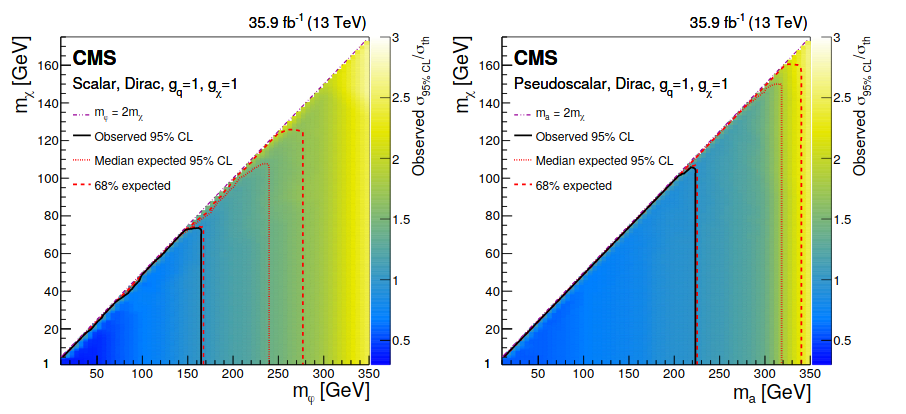
\includegraphics[width=16cm, height=6.5cm]{figs/CMSttbarExclusion.png}
\caption{95\% \ac{CL} exclusion plots on the signal strength computed as a function of the mediator and \ac{DM} masses obtained by \ac{CMS} considering a scalar (on the left) and a pseudoscalar (on the right) mediator for the interaction \cite{PreviousDoubleTopAllLep13CMS}.}
\label{figure:CMSttbarExclusion}
\end{center}
\end{figure}

Last year, a \ac{CMS} combination of the $t/\bar t$+DM and $t \bar t$+DM analyses has also been published \cite{PreviousSingleDoubleTopAllLep13CMS}, combining this time only the hadronic and semileptonic channels of both analyses. The limits obtained in this case are represented in Figure~\ref{figure:Combination2019}, where the limits obtained by each analysis on their own along with the results of the combination, leading to a factor 2 improvement of the limits obtained, have been represented. 

This combination managed to exclude the production of scalar mediators up to 290 GeV and pseudoscalar mediators up to 300 GeV, at the 95\% \ac{CL} for the couplings considered. This combined analysis actually leads to the most stringent exclusion limits of the \ac{LHC} on the production of \ac{DM} through these categories of spin-0 mediators.

\begin{figure}[htbp]
\begin{center}
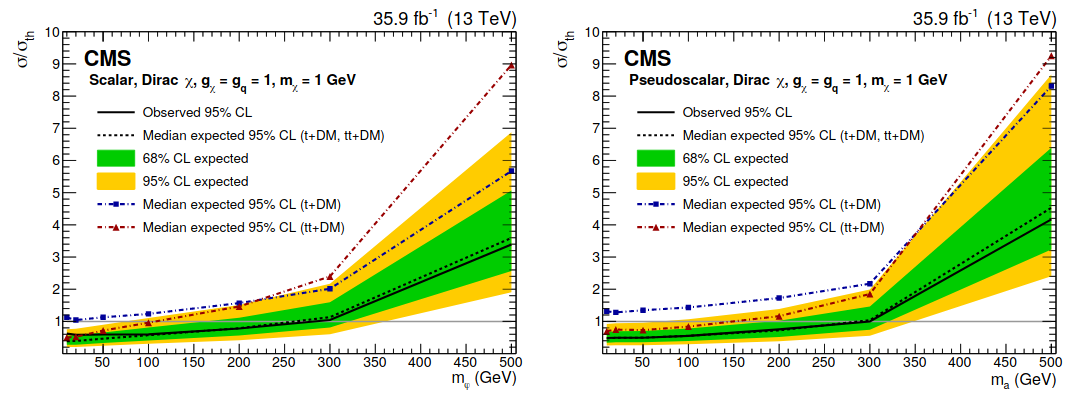
\includegraphics[width=16cm, height=6.5cm]{figs/Combination2019.png}
\caption{Expected and observed 95\% \ac{CL} limits on the \ac{DM} production cross sections shown considering scalar (on the left) and pseudoscalar (on the right) mediators for the interaction \cite{PreviousSingleDoubleTopAllLep13CMS}.}
\label{figure:Combination2019}
\end{center}
\end{figure}



























\chapter{The experimental setup} \label{chapter:Device}

The data analyzed throughout this work is the result of several years of proton-proton collisions produced at the \ac{LHC} with a center of mass energy of 13 TeV, and the particles emerging from these collisions have been recorded with the \ac{CMS} detector. In order to provide the experimental context of this thesis, the Section~\ref{section:LHC} of this section will be dedicated to the description of the accelerator, while the detector, in which thousands of people were involved and made of several different layers, will be described in Section~\ref{section:CMS}.

\section{The \acf{LHC} accelerator} \label{section:LHC}

The \acf{LHC} is a superconducting particle accelerator able to accelerate protons and lead ions up to velocities close to the speed of light (0.99999999c). Planned since the end of the 20th century, this accelerator, a 27 kilometers ring put 100 meters underground (under France and Switzerland) to avoid part of the contamination due to the cosmic rays and located at \ac{CERN}, has now been running for 10 years. The \ac{LHC} is the result of the collaboration between thousands of scientists of more than 100 different nationalities and its main objective was first of all to either infer or confirm the possible existence of the Higgs boson, theoretically predicted in the 1960s \cite{HiggsPostulate1, HiggsPostulate2} but never observed in any experiment. The discovery of the Higgs boson, announced at \ac{CERN} on the 4th of July 2012 \cite{HiggsDiscovery1, HiggsDiscovery2}, was then a magnificent achievement of the accelerator, after only a few years years of operation.

Now that the Higgs boson has been discovered, the priority of the \ac{LHC} shifted a bit. Even though many different teams are still studying this particle in order to determine precisely its most fundamental properties such as its mass, couplings or spin, many groups of scientists are involved in different kinds of \ac{BSM} physics since the \ac{LHC}, whose center of mass energy has kept increasing over the years, allows us to reach a level of energy never reached before and therefore allows us to probe new parts of the phase space, searching for eventual hints of new physics. These kind of searches of course include the search for \ac{DM} production as the one performed in this work. 

%Let's now start with a global description of the general design of this particle accelerator in Section~\ref{section:LHCNut} before describing in more details the key parameters allowing us to evaluate its actual performances in Section~\ref{section:LHCParams}.

\subsection{The \acs{LHC} in a nutshell}\label{section:LHCNut}

The \ac{LHC} is an underground particle accelerator built in the same 27 kilometers tunnel where the \ac{LEP} was previously used \cite{LEP}. This machine is accelerating two beams made out of ~$10^{10}$ protons or ~$7\cdot10^{7}$ lead ions in each direction and is mostly made out of more than 4000 superconducting magnets, in majority dipoles and quadrupoles, allowing respectively to curve the beam to maintain a nominal circular trajectory and to focus it by compensating its natural dispersion due to the repulsion of the protons making up these beams. A dedicated small section of the accelerator is then made out of 16 radio-frequency cavities synchronized in such a way that these protons always face a negative electric charge, which is used as the driving process of the actual acceleration of such particles.

Once the nominal center of mass energy $\sqrt{s} = 13$ TeV is reached (this concept will be described in Subsection~\ref{subsection:CMEnergy}), the protons are then smashed together in four different places on the \ac{LHC}, where the four detectors (\ac{ATLAS}, \ac{CMS}, \ac{ALICE} and LHCb) have been placed in order to study the collisions. Both \ac{ATLAS} and \ac{CMS} are general detectors able to study exotic processes such as the production of \ac{DM} and to make precision measurements on \ac{SM} physics as well (the decision to build two separate detectors was made in order to introduce some redundancy and to check the results). \ac{ALICE} on the other hand is mostly dedicated to the study of heavy ions collisions that happen $\sim 10$\% of the time in order to study in particular a specific state of matter, called quark-gluon plasma \cite{ALICE}. Finally, LHCb has been designed to study in particular the CP violation phenomena, which could be the sign of some new physics \cite{LHCb}.

It is important to note at this point that the \ac{LHC} is not a standalone accelerator in the sense that protons enter the \ac{LHC} with a velocity already close to the speed of light. In order to reach such input energies ($\sim 450$ GeV), previous smaller accelerators of \ac{CERN} are still used today. A chain of accelerators is then formed: first of all, the protons, extracted from a bottle of ordinary hydrogen, are injected into the LINAC 2, a linear accelerator, before being transferred to the \ac{PS}, the \ac{SPS} and finally the \ac{LHC} itself (all this chain of acceleration can be found in Figure~\ref{fig:Chain}).

\begin{figure}[htbp]
\begin{center}
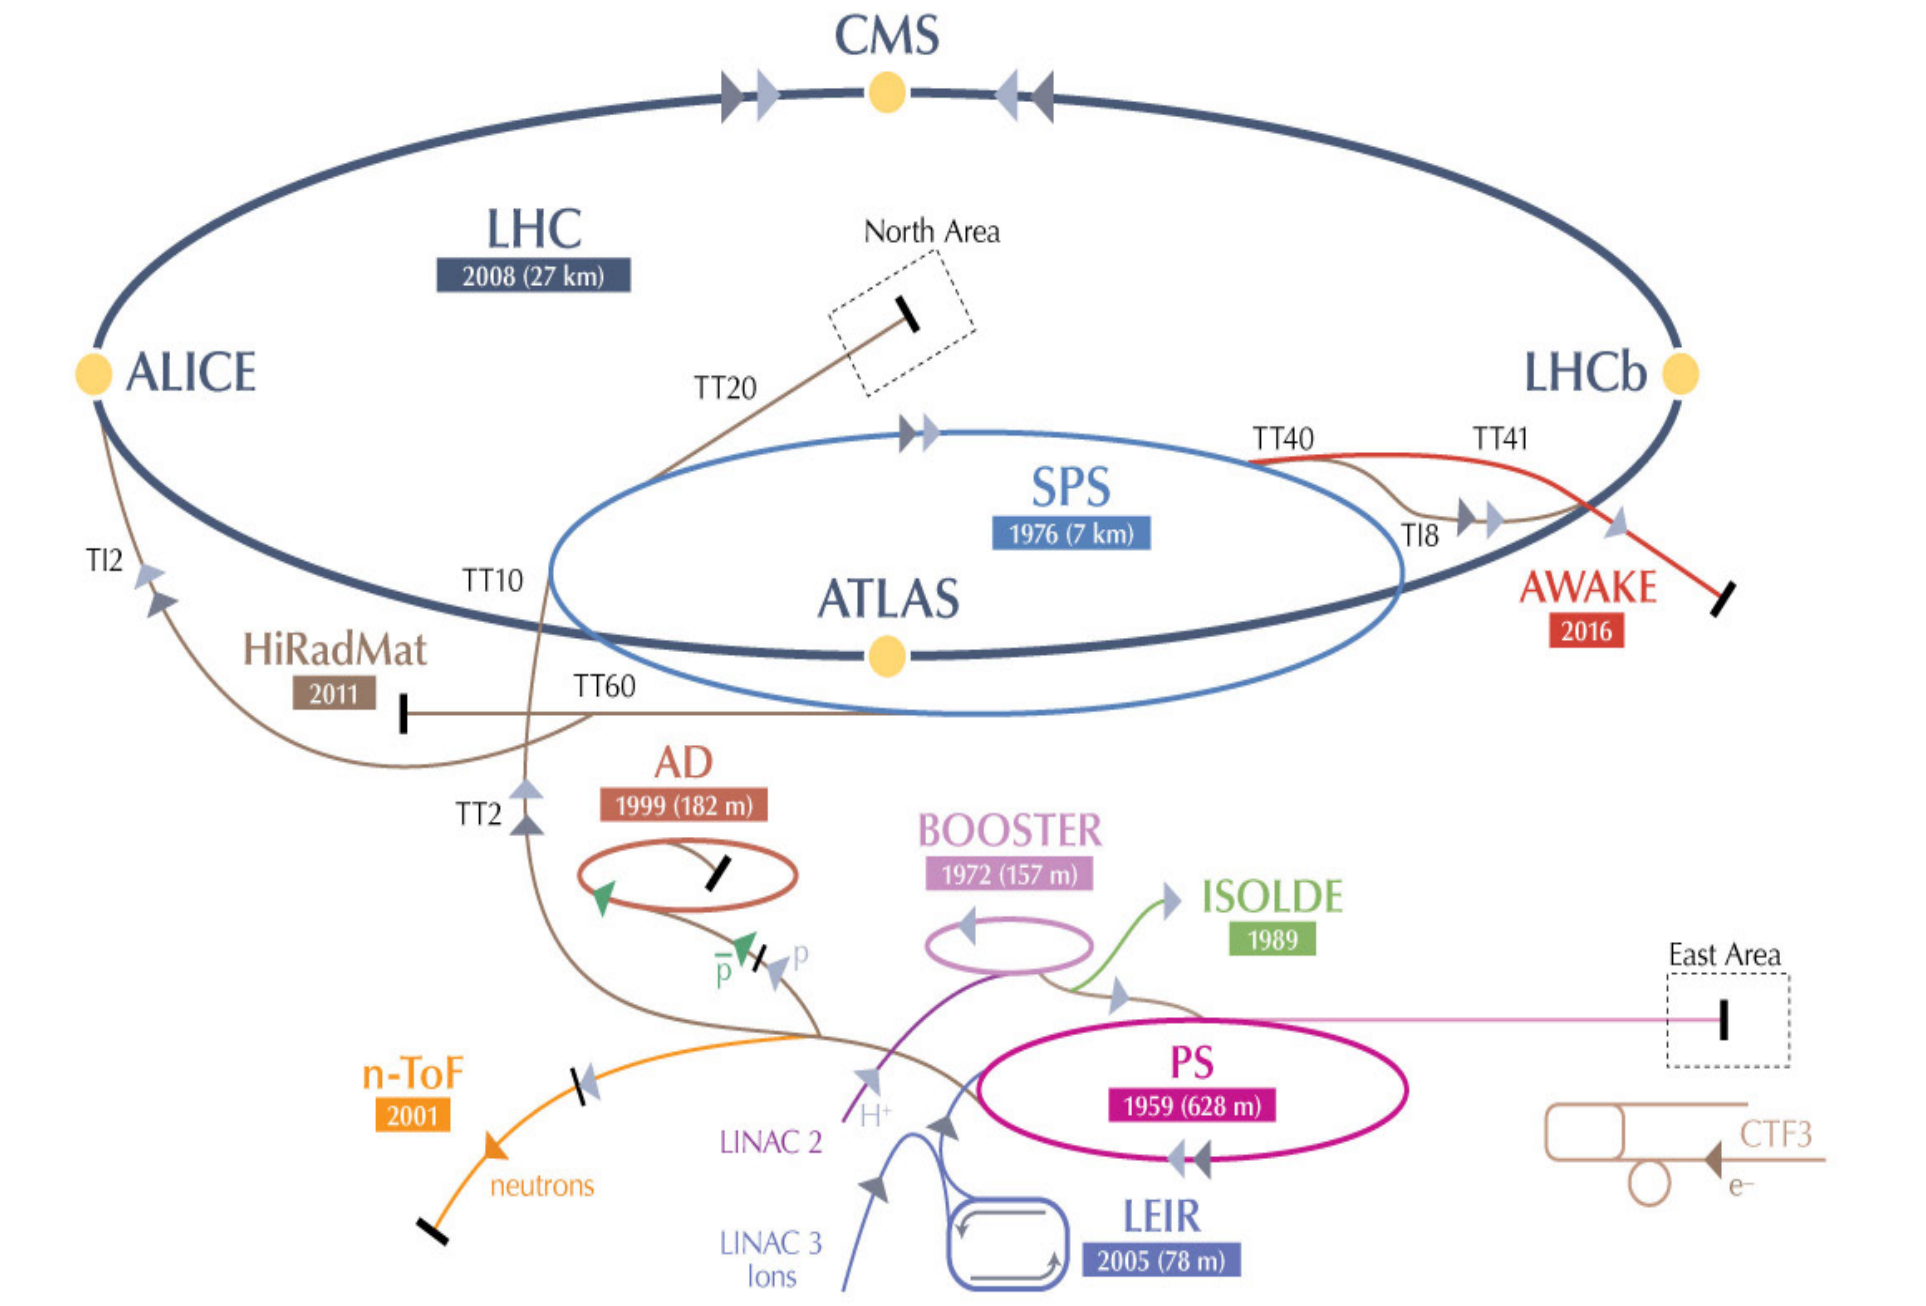
\includegraphics[width=12cm, height=8cm]{figs/LHCChain.png}
\caption{LHC injection chain and experiments performed at \ac{CERN} \cite{AWAKE}.}
\label{fig:Chain}
\end{center}
\end{figure}

During this phase of acceleration, the beam is separated in 2808 bunches of protons nominally separated by 25ns (giving a collision rate of 40 MHz), so that the experiments have the time to record the collision, clean the detectors and get ready for the next bunch crossing, coming just a few nanoseconds later. Each time one bunch crossing happens, around 30-35 collisions of protons happen at once, on average: this phenomena, usually referred to as \ac{PU}, has to be taken into account as well and will be described in the next section.

As previously stated, the amount of data collected is a crucial parameter for many analyses, meaning that the \ac{LHC} would ideally need to run 24 hours a day, 365 days per year in order to maximize the data taking. However, this is typically not possible, as setting up a beam takes time and we cannot keep it rotating at maximal energy in the machine for a long time so in ideal conditions, around 20 hours of data taking a day are expected. The \ac{LHC} is then running around 9 months per year, being usually stopped during winter for maintenance operations, and the data taking periods are defined into Runs of a few years, after which the accelerator is usually stopped for a longer period of time, a \ac{LS}, in order to also have the time to perform additional upgrade operations of the machine. 

The data analyzed in this work corresponds to the second phase of the Run II of operation of the \ac{LHC}, from 2016 to 2018, while the Run III is now expected to start in the Spring of 2021. The summary of the main parameters of operation of the \ac{LHC} across the different Runs of operations can be found in Table~\ref{table:LHCRuns}.

\begin{table}
\begin{center}
\begin{tabular}{ c|c|c|c|c } 
 \hline
 Parameter & Run I & Run II & Run III & Design \\
\hline
Energy [TeV] & 7 $\rightarrow$ 8 & 13 & 13 & 14 \\
Bunch spacing [ns] & 50 & 25 & 25 & 25 \\
Intensity [$10^{11}$ protons per beam] & 1.6 & 1.2 & Up to 1.8 & 1.15 \\
Bunches & 1400 & 2500 & 2800 & 2800 \\
Emittance [$\mu m$] & 2.2 & 2.2 & 2.5 & 3.5 \\
$\beta^*$ [cm] & 80 & 30 $\rightarrow$ 25 & 30 $\rightarrow$ 25 & 55 \\
Crossing angle [$\mu$rad] & - & 300 $\rightarrow$ 260 & 300 $\rightarrow$ 260 & 285 \\
Peak luminosity [$10^{34}$ cm$^{-2}$ s$^{-1}$] & 0.8 & 2.0 & 2.0 & 1.0 \\
Peak \ac{PU} & 45 & 60 & 55 & 25 \\
 \hline
\end{tabular}
\caption{ Expected and observed main parameters of $pp$ operation of the \ac{LHC} across the different eras of operation \cite{LHCRuns}.}
\label{table:LHCRuns}
\end{center}
\end{table}

\subsection{Key parameters}\label{section:LHCParams}

\subsubsection{Center of mass energy} \label{subsection:CMEnergy}

The center of mass energy is defined as a Lorentz invariant quantity under any kind of boost resulting of the collisions of two protons (defined as $E_1, \overrightarrow{p_1}, m_1$ and $E_2, \overrightarrow{p_2}, m_2$) with a $\theta$ angle, as developed in Equation~\ref{eq:CMEnergy}. It is a key variable of the \ac{LHC} since the phase space of particles that can be explored directly depends on this value.

\begin{equation}
\label{eq:CMEnergy}
\sqrt{s} = \sqrt{(m_1)^2 + (m_2)^2 + 2 \left (E_1 E_2-2 |\overrightarrow{p_1}| \text{ } |\overrightarrow{p_2}| \text{ cos}(\theta) \right )}
\end{equation}

The LHC started its operation in 2008 running at an energy of 7 TeV, quickly moved to 8 TeV and kept this level of energy during the end of the Run I of operation. In 2015, for the Run II of data taking, the energy was increased until reaching 13 TeV (2 times 6.5 TeV for each beam) and an expected value of 14 TeV, the nominal energy for which the \ac{LHC} was originally built, is expected to be reached in the near future.

\subsubsection{Luminosity} \label{subsection:Lumi}

The luminosity is another extremely important variable for the operation of the \ac{LHC} since it gives an indication on the number of collisions per second given by the accelerator. Increasing this parameter is then crucial to collect as much data as possible, in order to be able to isolate processes having a low production cross section and therefore an extremely low probability of creation when colliding two protons.

Mathematically, we can first of all define in Equation~\ref{eq:Rate} the rate of production $R$ (in number of events per second) of any given process using its cross section $\sigma$, equivalent to its production probability, and the instantaneous luminosity $\mathcal{L}$. From this rate can be extracted easily the number of expected interactions $N$ in a certain amount of time $T$ as well. 

\begin{equation}
\label{eq:Rate}
\begin{dcases}
R = \mathcal{L} \cdot \sigma \\
N(T) = \sigma \int_0^T \mathcal{L}(t) dt = \sigma L
\end{dcases}
\end{equation}

This instantaneous luminosity we just introduced $\mathcal{L}$ can be defined using Equation~\ref{eq:Luminosity}, assuming that the beams have a Gaussian profile, while the integrated luminosity $L$ can be defined by simply integrating the instantaneous luminosity over time $L = \int \mathcal{L}dt$ \cite{Thomson}.

\begin{equation}
\label{eq:Luminosity}
\mathcal{L} = \frac{\gamma f_{\text{rev}} k_B N_p^2}{4 \pi \epsilon_n \beta^*}G \text{,  where } G = \frac{1}{\sqrt{1+\frac{\theta_C \sigma_z}{2 \sigma}}}
\end{equation}

In this last equation, the following properties of the accelerator have been introduced, giving the \ac{LHC} a nominal instantaneous luminosity $\mathcal{L} = 10^{34}$ cm$^{-2}$ s$^{-1}$:
\begin{itemize}
\item $\gamma$ is the usual relativistic Lorentz factor (for the \ac{LHC}, when protons go at their maximum velocity of 99.9999991\% of the speed of light, $\gamma = 7460$)
\item $f_{\text{rev}}$ is the frequency of revolution (11.2 kHz)
\item $k_B$ is the number of proton bunches per beam (2808 for a 25ns bunch spacing)
\item $N_p$ is the number of protons per bunch ($1.15 \cdot 10^{11}$ protons)
\item $\epsilon_n$ is the transverse normalized emittance (3.75 $\mu$m)
\item $\beta^*$ is the betatron function at the interaction point (0.55 m)
\item $G$ is the geometrical factor accounting for the fact that the collisions do not happen exactly head-on, therefore reducing the effective luminosity, expressed from the full crossing angle between colliding beam $\theta_C$ (285 $\mu$rad), and $\sigma$, $\sigma_z$, the transverse and longitudinal r.m.s. sizes (respectively 16.7 $\mu$m and 7.55 cm).
\end{itemize}

As previously stated, increasing the luminosity of the \ac{LHC} is always something interesting in order to produce processes having a low production cross-section, and we can then see that many different parameters can be tweaked in order to achieve the highest possible instantaneous luminosity, such as the number of protons per bunch, the number of bunches per beam or the beam crossing angle at the interaction point. New radio-frequency crab cavities will probably be installed during the next \ac{LS} of the \ac{LHC} in order to increase the value of the geometrical factor $R$ and the instantaneous luminosity by a factor $\sim 10$ (HL-LHC project \cite{HLLHC}).

The total integrated luminosity taken by the \ac{LHC} during its different years of operation has been summarized in Figure~\ref{fig:Lumi}. The final datasets available for the Run II and analyzed in this work have an integrated luminosity of ($35.9 \pm 0.9$)~fb$^{-1}$ (2016), ($41.5 \pm 1.0$)~fb$^{-1}$ (2017) and ($59.7 \pm 1.5$)~fb$^{-1}$ (2018), resulting in a total dataset of ($137.1 \pm 2.0$)~fb$^{-1}$ recorded during the Run II of operation. This roughly means that we expect to have produced around 137 events of any process whose cross section of production would be equal to 1~fb.

\begin{figure}[htbp]
\begin{center}
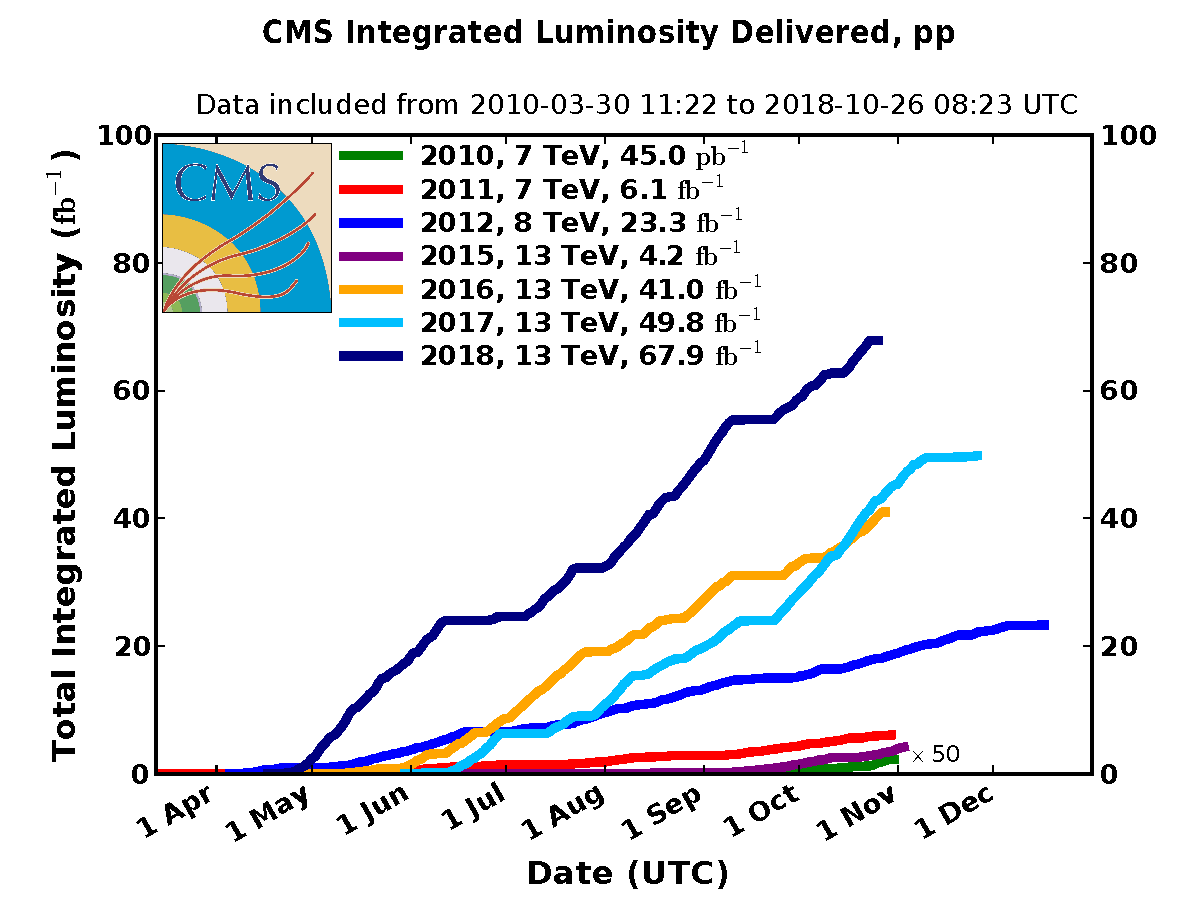
\includegraphics[width=12cm, height=8cm]{figs/CumuLumi.pdf}
\caption{Integrated luminosity collected by \ac{CMS} over its different years of operation so far.}
\label{fig:Lumi}
\end{center}
\end{figure}

\subsubsection{Number of simultaneous interactions: \acf{PU}} \label{subsection:PU}

The last key parameter of the \ac{LHC} discussed here is the number of simultaneous interactions, also called \ac{PU}. Usually, because of the high density of protons within the beams, a bunch crossing in an experiment produces around 30-35 proton collisions, as seen in Figure~\ref{fig:PU}, defining the \ac{PV} as the most interesting one, while the other vertices are usually referred to as the \ac{PU}. The tracker of \ac{CMS}, which will be introduced in Section~\ref{subsection:Tracker}, therefore needs to be able to reconstruct all these events in order to define the \ac{PV} of the interaction. 

\begin{figure}[htbp]
\begin{center}
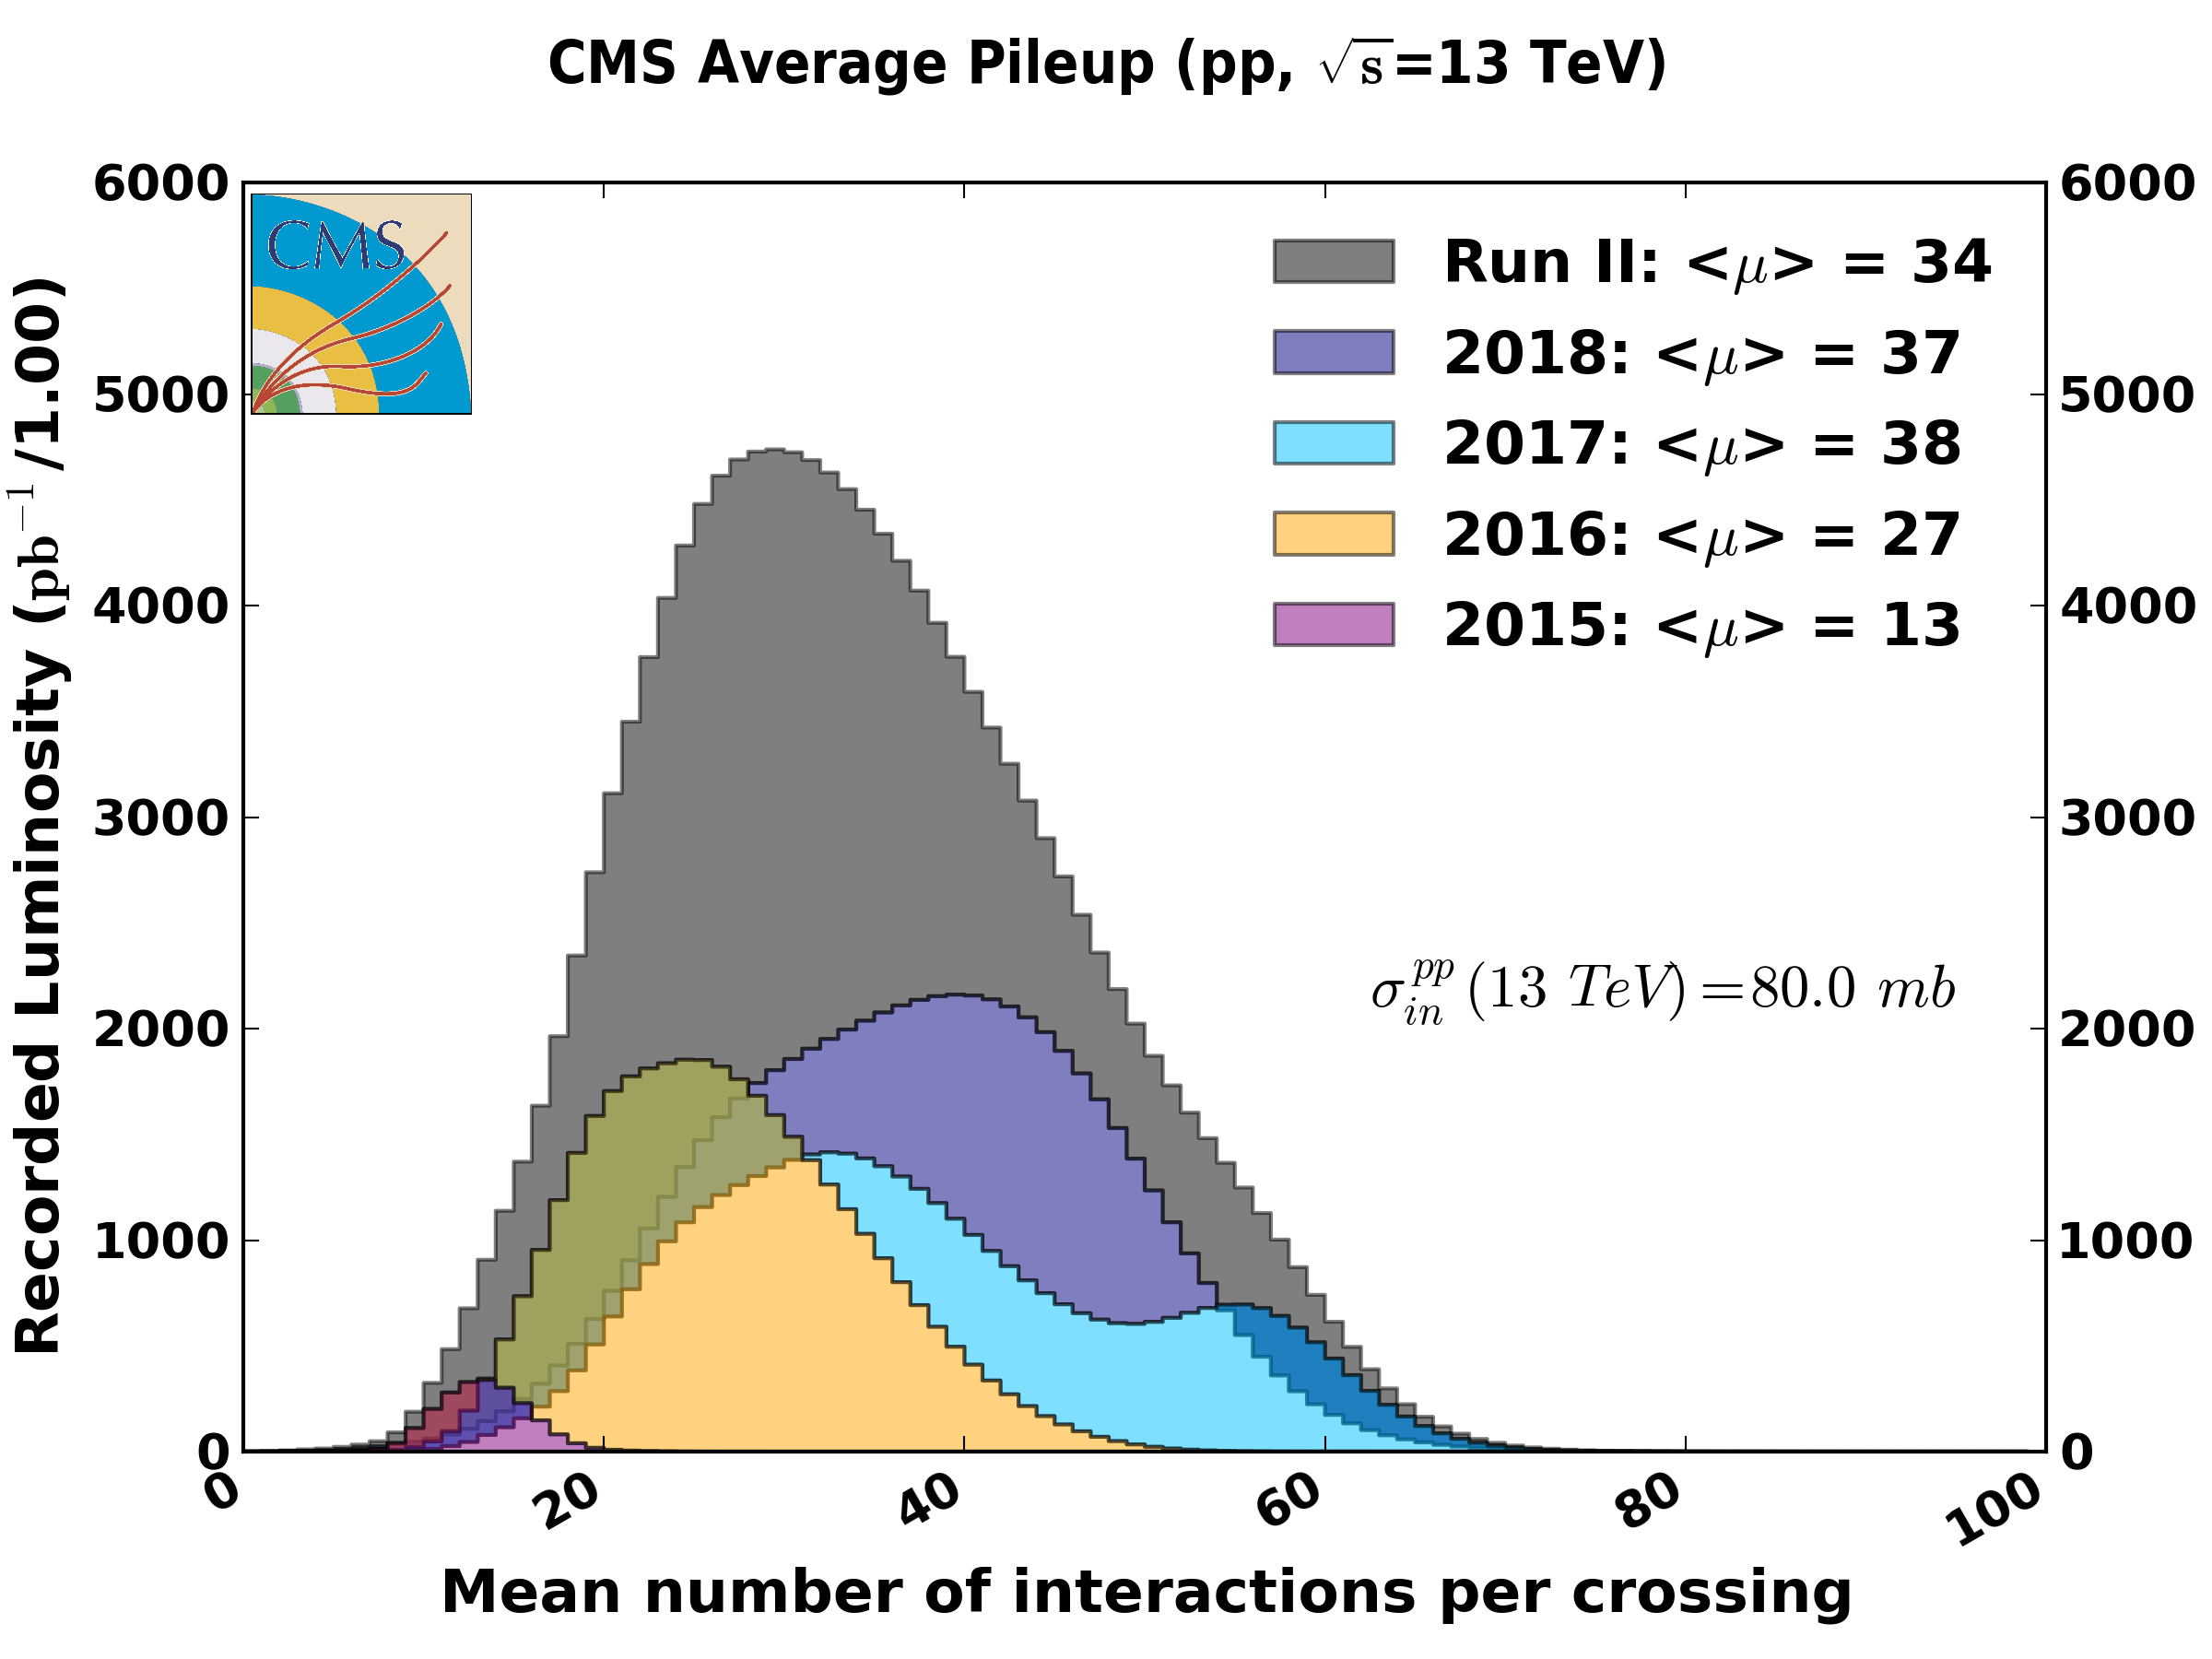
\includegraphics[width=12cm, height=8cm]{figs/PUSummary.png}
\caption{Mean \ac{PU} distribution and luminosity recorded by \ac{CMS} over the different years of operation of the \ac{LHC}.}
\label{fig:PU}
\end{center}
\end{figure}

\section{The \ac{CMS} detector} \label{section:CMS}

The \acf{CMS} is one of the two general purpose detectors of the \ac{LHC} and is installed at the access point 5 of the \ac{LHC}. Its main purposes are to discover the Higgs boson, make precision measurement of its properties and also of other \ac{SM} processes and to discover \ac{BSM} physics, such as the possible existence of \ac{DM}. 

\ac{CMS} has been carefully designed by hundreds of different physicists and engineers in order to be as hermetic as possible, covering all the possible angles around the beam pipe. It therefore counts with a central part with cylindrical shape, the barrel, and two endcaps, one on each side of the detector. With its 14.000 tons, distributed over a diameter of 15 meters and a length of 28.7 meters, the detector can be considered quite compact and was lowered into the experimental cavern after being built on the surface in 14 different moving pieces, a flexible design allowing to access its inner parts, by opening and closing the detector when needed.

\subsubsection*{\acs{CMS} subdetectors}

As shown in Figure~\ref{fig:CMS}, \ac{CMS} is made out of different layers corresponding to different subdetectors, each able to provide different kinds of information about the particles created by each collision \cite{CMSDescription}. These subdetectors will be described in detail in the following sections, but they have all been designed in order to make the reconstruction of the different events efficient, fast and precise while matching the tight conditions occurring at the \ac{LHC}.

\begin{figure}[htbp]
\begin{center}
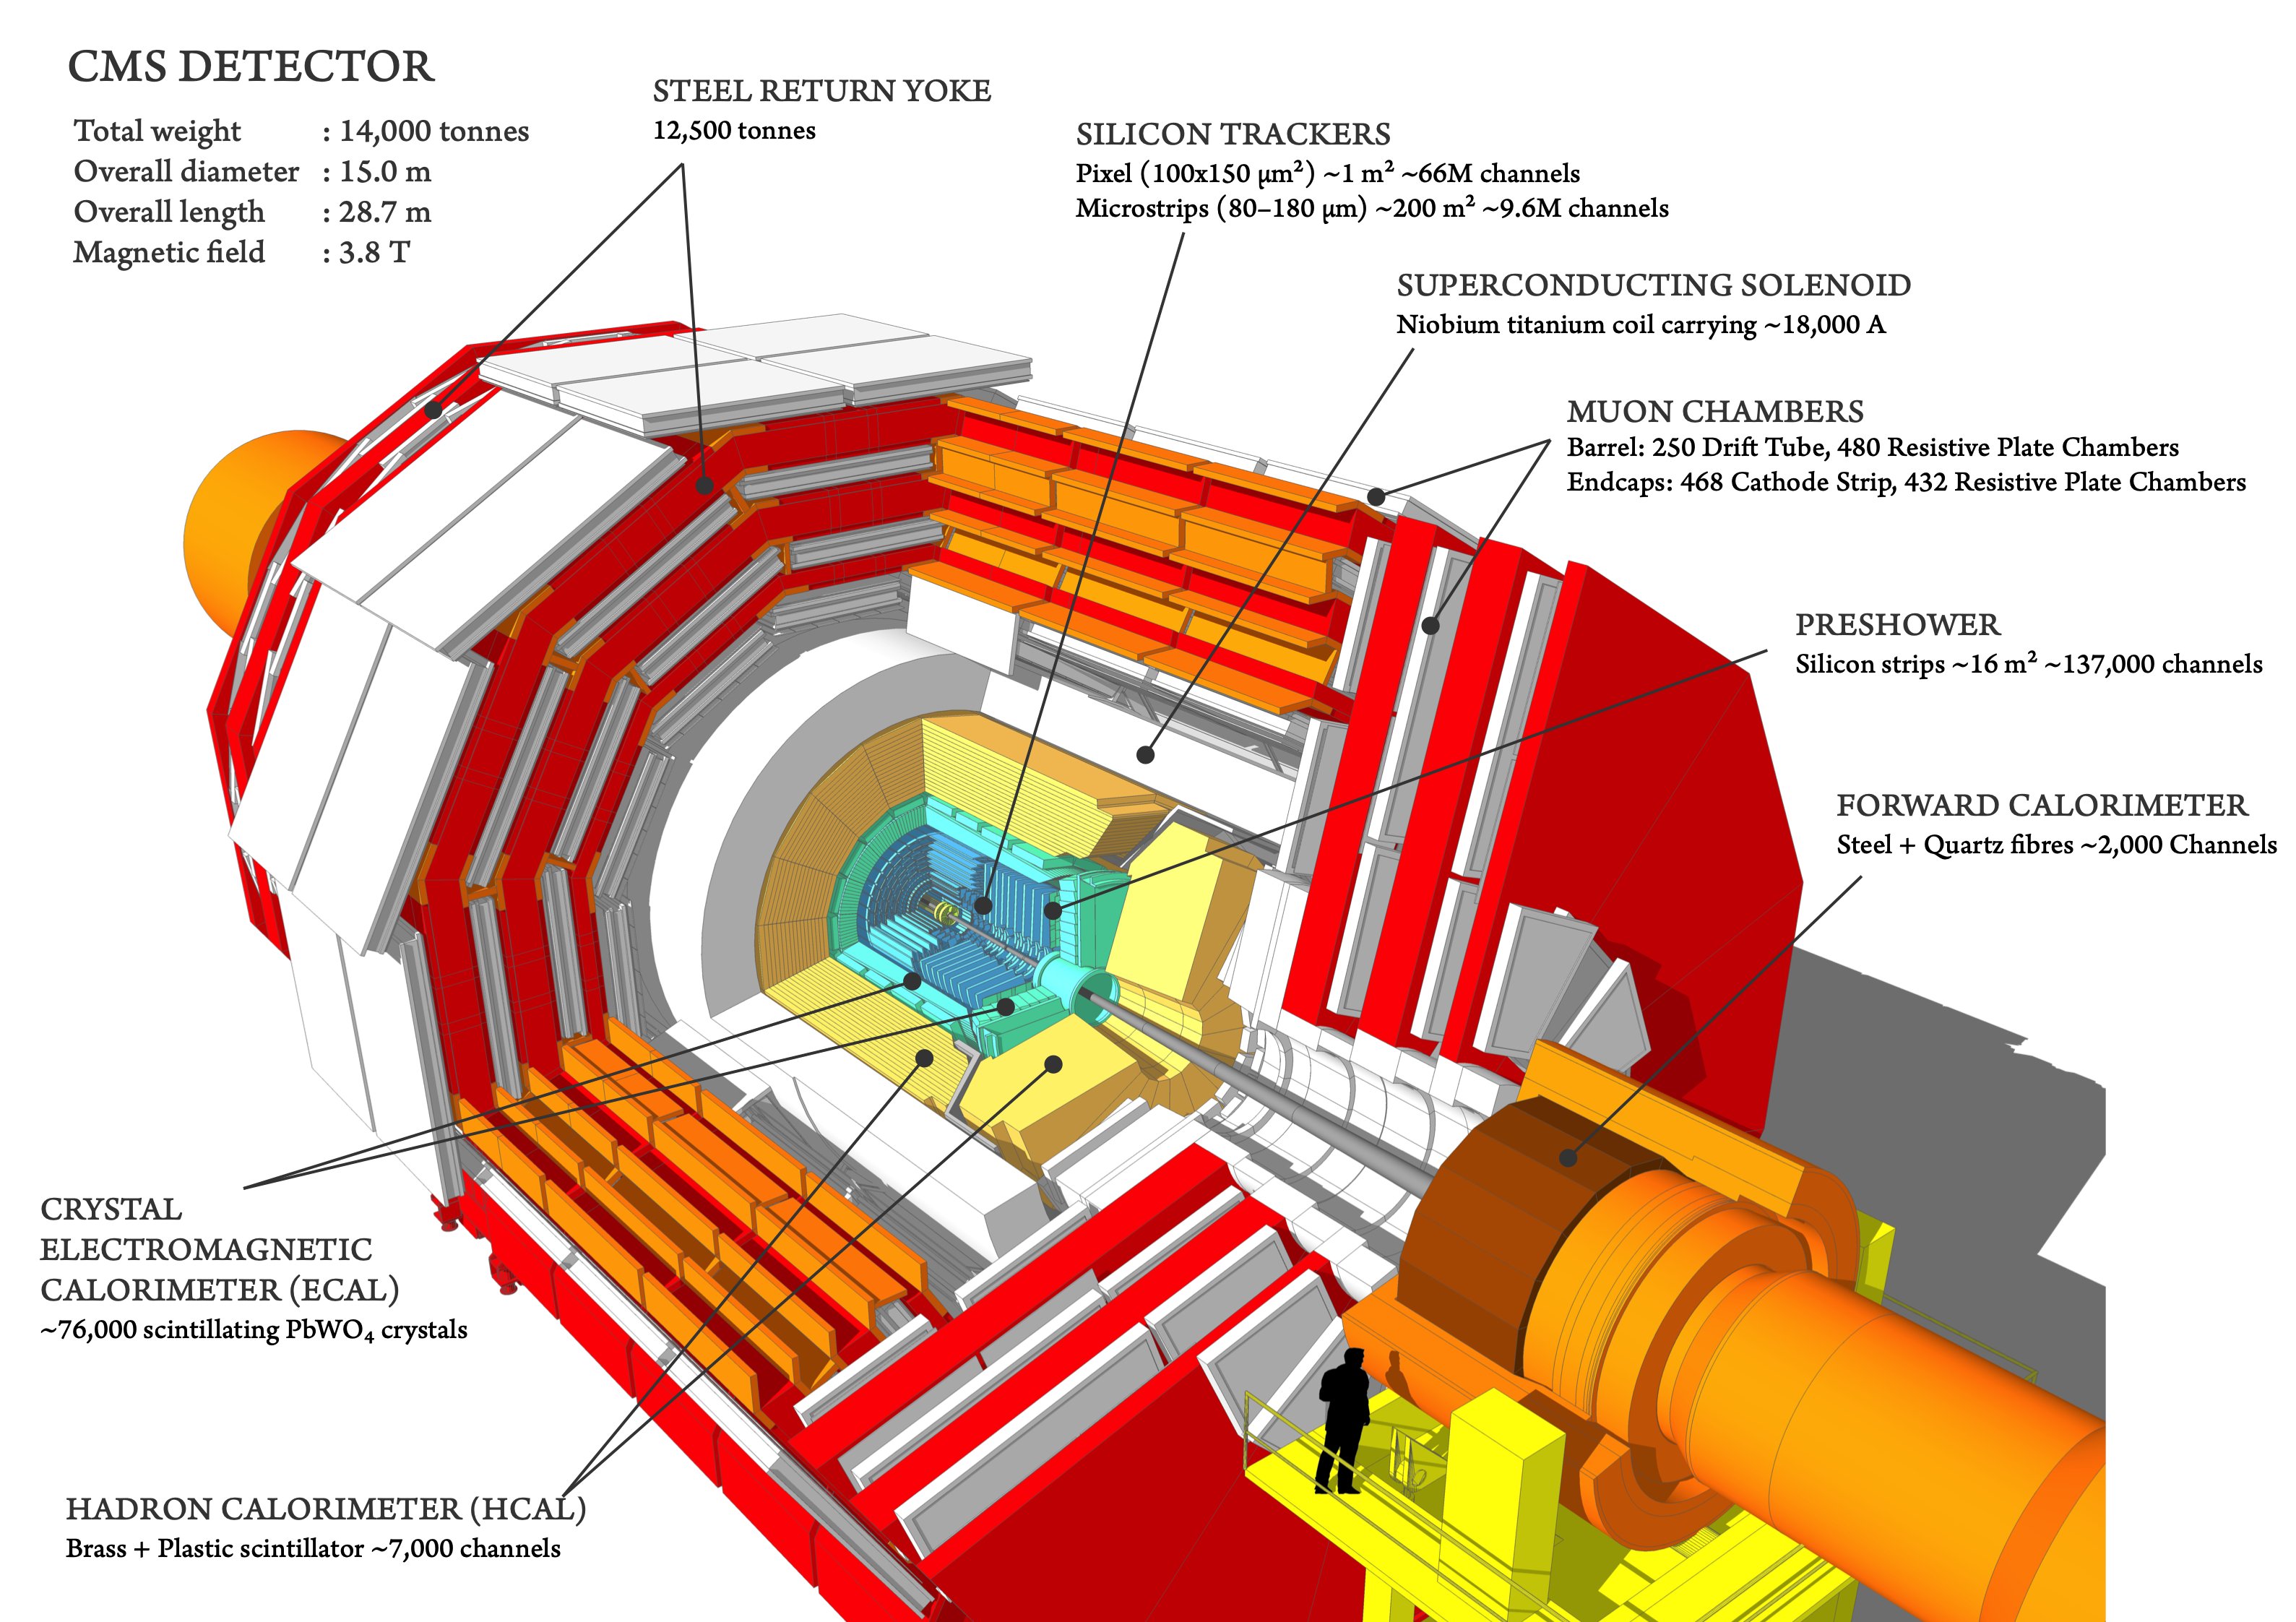
\includegraphics[width=15cm, height=10cm]{figs/CMS.png}
\caption{Schematic representation of the \ac{CMS} detector, along with all its subdetectors and main characteristics.}
\label{fig:CMS}
\end{center}
\end{figure}

The inner part of the \ac{CMS} detector is the so-called tracker, a device made out of silicon pixels and strips, described in Section~\ref{subsection:Tracker} and responsible for the precise reconstruction of all the charged particles coming from the different interaction vertices. A bit further, the \acf{ECAL} can be found, made out of thousands of crystals as described in Section~\ref{subsection:ECAL} and used to precisely measure the energy of particles able to interact electromagnetically by producing an electromagnetic shower that can be detected. Then, the \acf{HCAL} comes, described in Section~\ref{subsection:HCAL} and whose main purpose is to identify and measure the main properties of the hadrons produced in the collisions.

The \ac{CMS} name partly comes from its central piece, a huge superconducting solenoid described in Section~\ref{subsection:Solenoid} and able to produce a 3.8 T magnetic field in the detector, with a magnetic flux density increased even more by the addition of the steel return yoke layers (red parts in Figure~\ref{fig:CMS}). This magnetic field is essential in the sense that it is able to deflect the charged particles which have been produced via the Lorentz interaction, therefore giving us a way to measure their charge and energy from the measurement of the curvature of the induced binding.

Finally, on the outside of the detector the complete muon system can be found and particularly performing in \ac{CMS}. This subdetector is currently made out of three main sub-systems (the \acp{DT}, \acp{CSC} and \acp{RPC}), as explained in Section~\ref{subsection:Muon}, and is responsible for the identification and measurement of the momentum of the muons produced by the collisions.

\subsubsection*{Coordinates system}

%Before starting with the description of all these subdetectors, it is important to detail the coordinates system typically used within the \ac{CMS} collaboration. 
As a convention, is has been decided to use within the \ac{CMS} collaboration a right-handed Cartesian coordinate system with the origin defined as the interaction point, and with an x-axis pointing towards the center of the ring, an y-axis pointing upwards and a z-axis pointing towards the Jura mountains (along the counterclockwise beam direction), as represented in Figure~\ref{fig:CMSAxis}. 

\begin{figure}[htbp]
\begin{center}
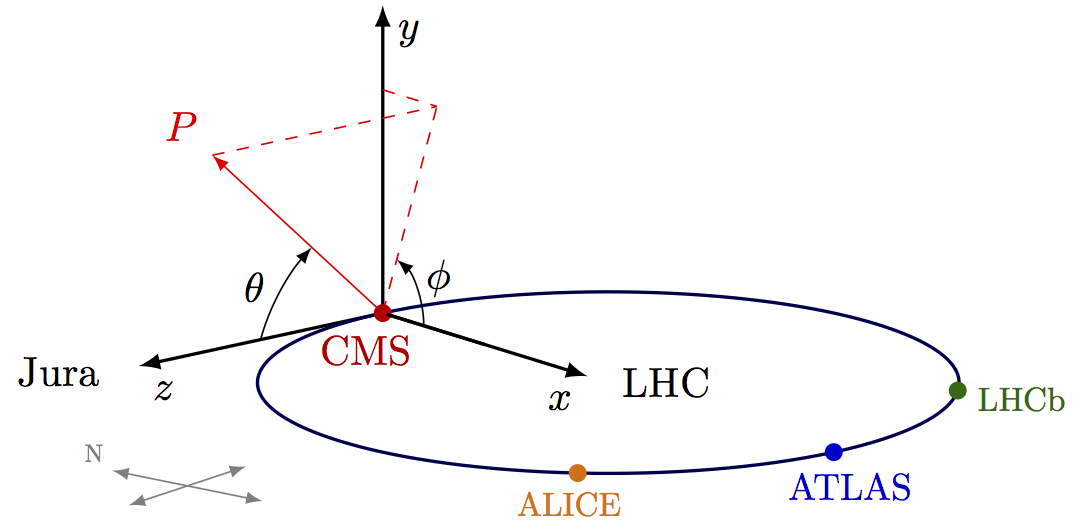
\includegraphics[width=12.2cm, height=6.5cm]{figs/CMSAxis.png}
\caption{Schematic representation of the \ac{CMS} coordinate system used by convention.}
\label{fig:CMSAxis}
\end{center}
\end{figure}

The $\theta$ and $\phi$ angles are then defined as the angles between the z and y axes and the x and y axes respectively and the pseudorapidity $\eta$, defined in Equation~\ref{eq:Pseudorapidity}, a Lorentz invariant quantity under boosts quite often used in the different analyses since the multiplicity of high energy particles is roughly expected to be constant in $\eta$.

\begin{equation}
\label{eq:Pseudorapidity}
\eta = - \text{log} \left (\text{tan} \left (\frac{\theta}{2} \right ) \right )
\end{equation}

\subsection{Tracker} \label{subsection:Tracker}

The tracker is the innermost part of the \ac{CMS} detector, is 5.4 meters long and has a diameter of 2.5 meters. Its main purpose is the reconstruction of the trajectories of charged particles issued from the primary and secondary interaction vertices in a quick and precise way in order to identify them and measure their individual momentum. 

Many challenges were faced when designing this system mainly because of the hard conditions provided by the \ac{LHC}. First of all, at its nominal instantaneous luminosity, an average of 1000 particles are created after each bunch crossing, every 25 nanoseconds. The tracking system then needs to read all its channels extremely fast in order to be ready for the next bunch crossing. However, this fast electronics then needs some cooling to work optimally, which would in return increase the size of the tracker and therefore increase the interactions between the detector and the particles created (by multiple scattering, bremsstrahlung, photon conversion and nuclear interactions). This would affect the trajectory of the particles so a compromise had to be found between the velocity and size of the tracker. Finally, this device needs to be resistant to the extreme radiation environment for its expected lifetime of at least 10 years.

This device is then made out of silicon pixels and strips mainly because of the granularity, reading velocity and radiation hardness offered by such material. It has been set up on several different layers disposed in such a way to make the detector as hermetic as possible, as shown in Figure~\ref{fig:CMSTracker}. A charged particle crossing the tracker will then leave a hit each time it crosses one of the silicon sensors, from which the track of the particle can be reconstructed using reconstruction algorithms that will be detailed in Chapter~\ref{chapter:Reco}.

\begin{figure}[htbp]
\begin{center}
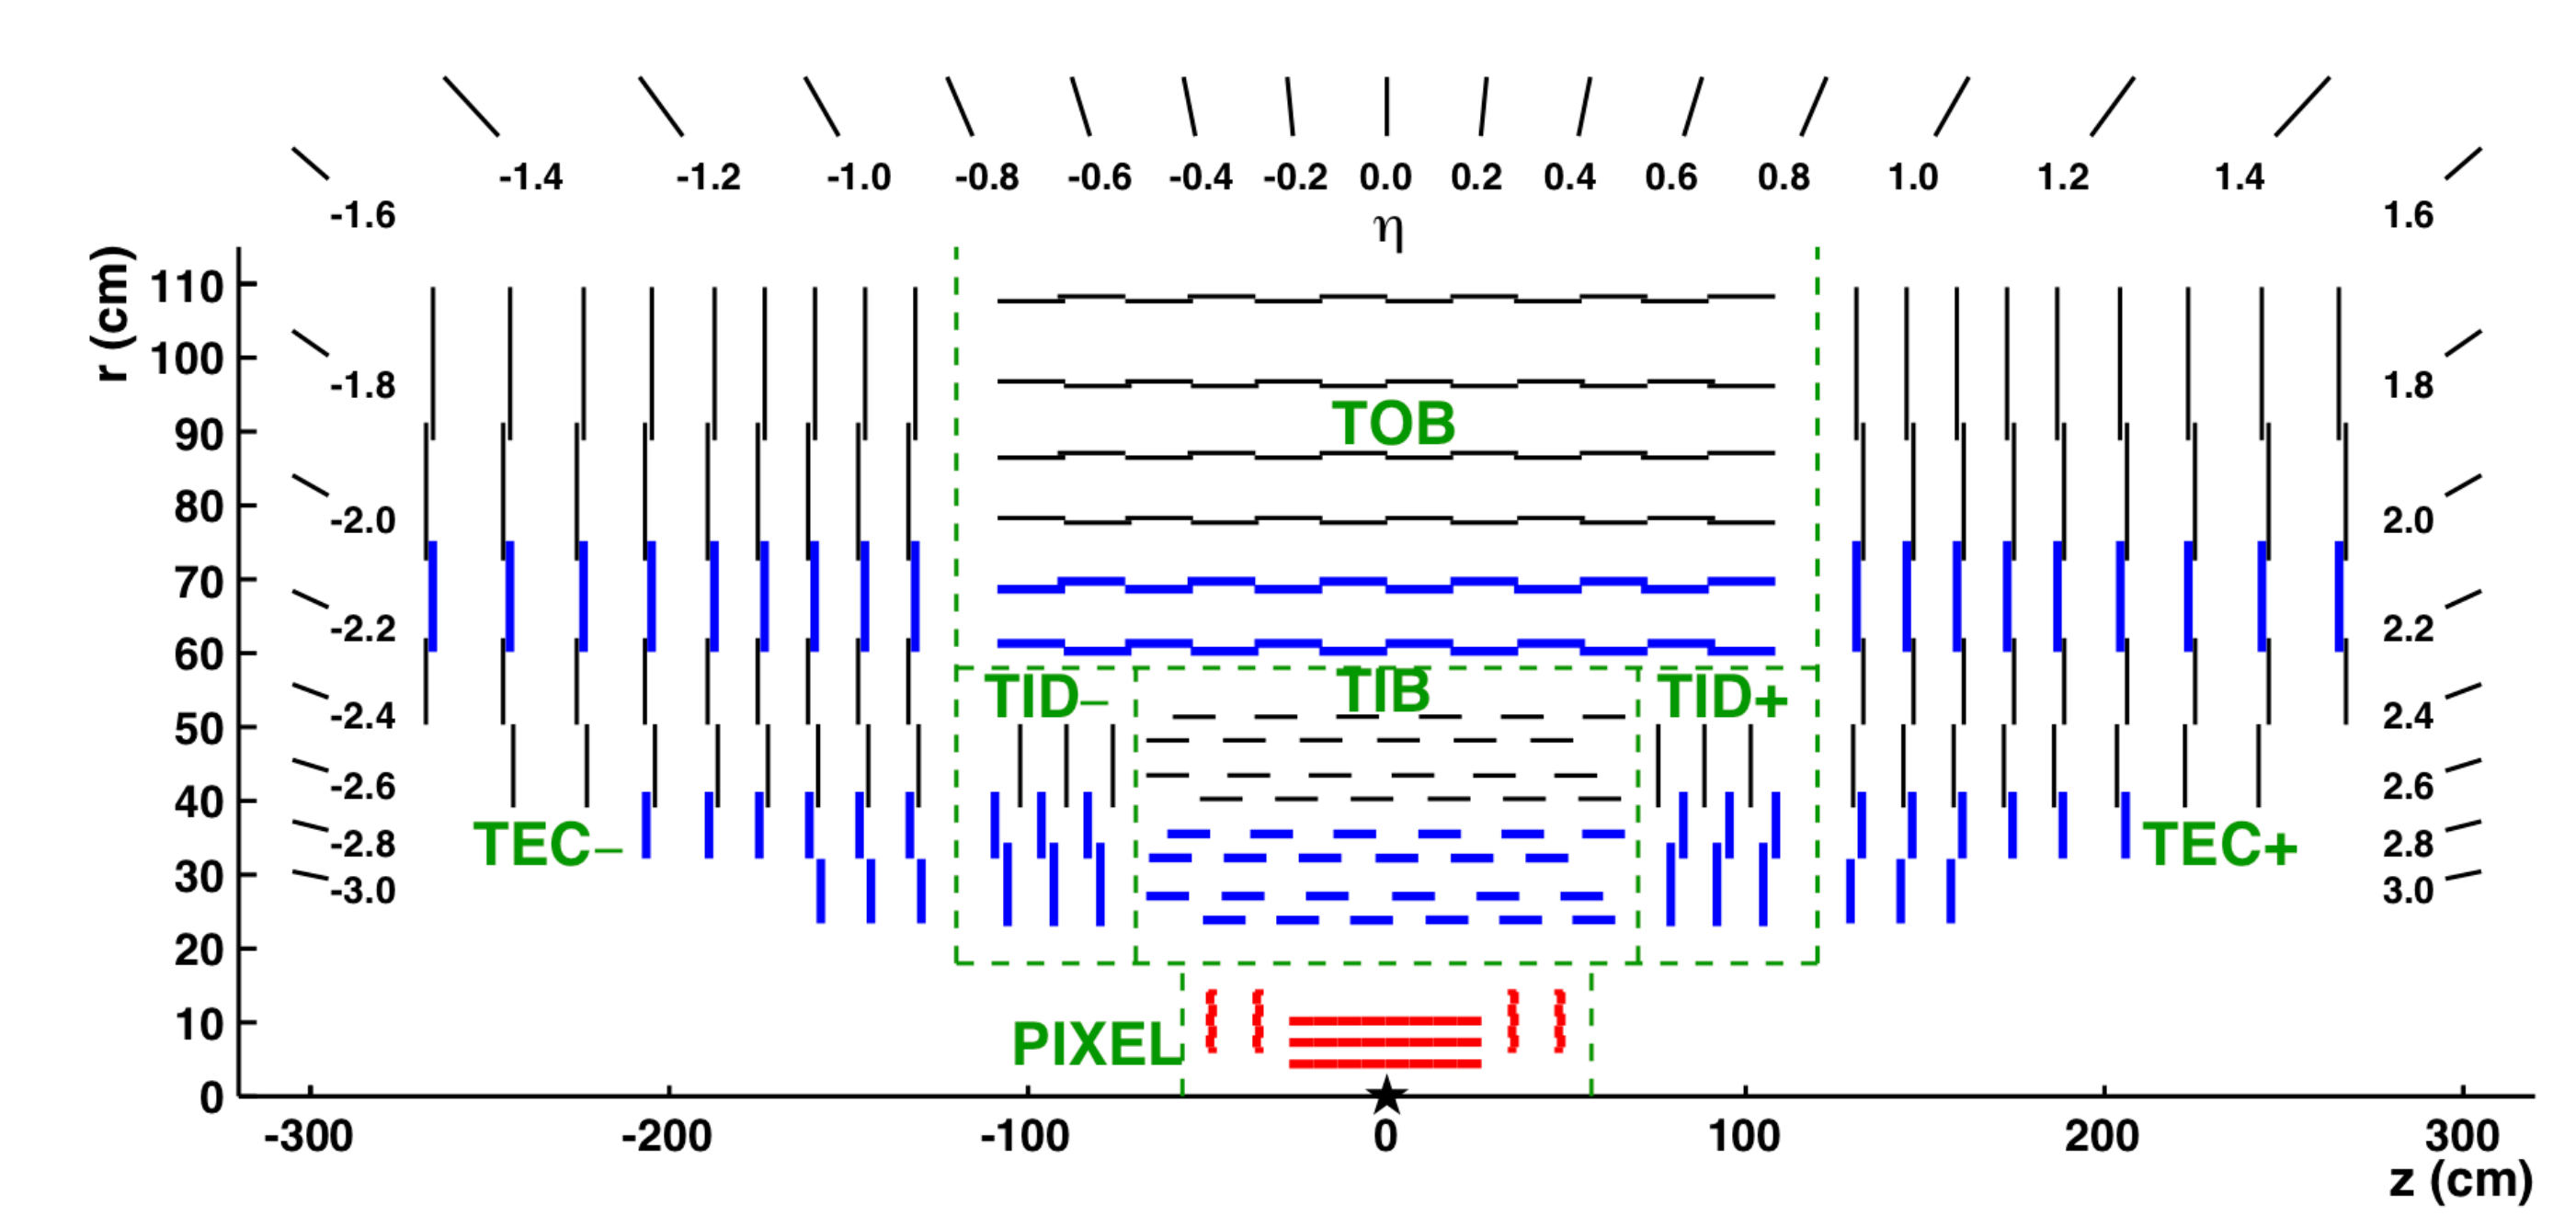
\includegraphics[width=14cm, height=7.2cm]{figs/CMSTracker.png}
\caption{Schematic representation of the \ac{CMS} tracker, for different pseudorapidity values and along the z-axis \cite{CMSTracker}.}
\label{fig:CMSTracker}
\end{center}
\end{figure}

The presence of the magnetic field due to the solenoid can then help us estimate the momentum of the particle, since the Lorentz force applied on such particle will introduce a deviation directly proportional to its momentum. The radius of curvature of particles with a high momentum ($> 100$ GeV) is really large but the density of pixels and the algorithm can still manage to estimate the momentum of such particles, even though the uncertainty associated will then be greater.

In particular, the tracker is made out of two distinct parts: the smaller and inner pixel detector and the larger silicon strip detector:

\begin{itemize}
\item The \textbf{pixel detector} is made out of three barrel pixel layers and two endcap disks for hermeticity (located at radii $r=4.4, 7.3$ and 10.2 cm of the \ac{PV}), one on each side. In total, more than 60 millions pixels make up the 1440 modules of this detector, covering an area corresponding to $\sim 1$ m$^2$.
\item The \textbf{silicon strip detector} on the other hand is composed of three different sub-systems, as seen in Figure~\ref{fig:CMSTracker} and covers a total area of $\sim 200$ m$^2$. First of all, the \ac{TIB/TBD} add an additional 4 barrel layers and 3 endcap disks to the tracker system up to a distance $r = 55$ cm to the \ac{PV} of the interaction, using silicon micro-strip sensors parallel in the barrel and perpendicular to the beam axis in both endcaps. Then, the \ac{TOB} surrounds this first layer; having an outer radius of 166 cm and going up to 118 cm along the z-axis, it adds 6 layers to the inner tracking system. Finally, the \acp{TEC} are made out of 9 disks and complete the measurement of particles emitted along the z-axis and having a high pseudorapidity $\eta$.
\end{itemize}

The \ac{CMS} tracker is extremely performing: one can see first of all in Figure~\ref{fig:TrackerRes} that for high momentum tracks of 100 GeV, the resolution is 1-2\% up to $|\eta| <$ 1.6. 

\begin{figure}[htbp]
\begin{center}
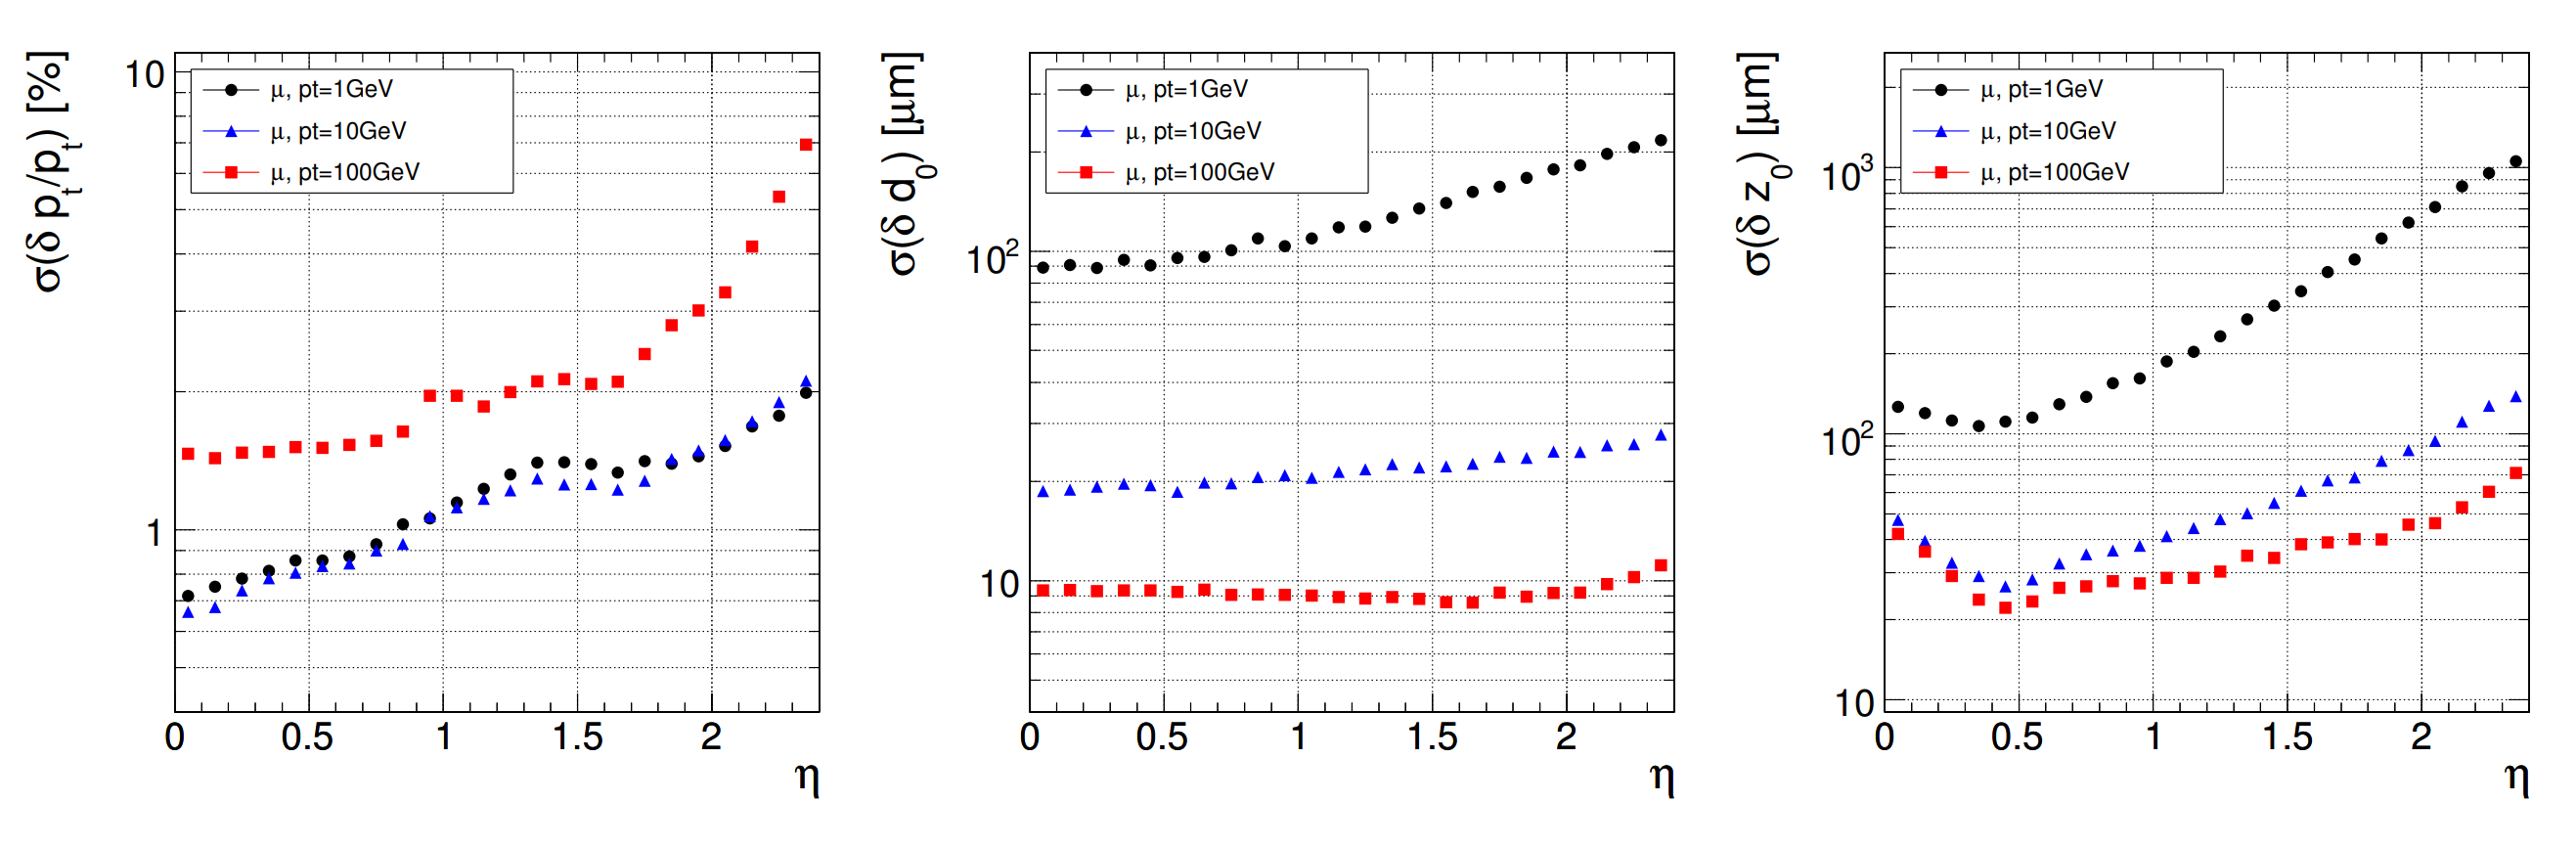
\includegraphics[width=15cm, height=5cm]{figs/TrackerRes.png}
\caption{Expected resolution of muons transverse momentum (left), transverse impact parameter (middle) and longitudinal impact parameter (right), as a function of pseudorapidity and muon momentum (1, 10 and 100 Gev) \cite{CMSDescription}.}
\label{fig:TrackerRes}
\end{center}
\end{figure}

Additionally, Figure~\ref{fig:TrackerEff} shows that muons are reconstructed with an efficiency higher than 99\% for most of the pseudorapidity spectrum, even though this efficiency drops at high $\eta$ values mainly because of the reduced coverage provided by the pixel forward disks. The interactions between the hadrons and the tracking system is also a bit higher, which results in a lower reconstruction efficiency for such particles.

\begin{figure}[htbp]
\begin{center}
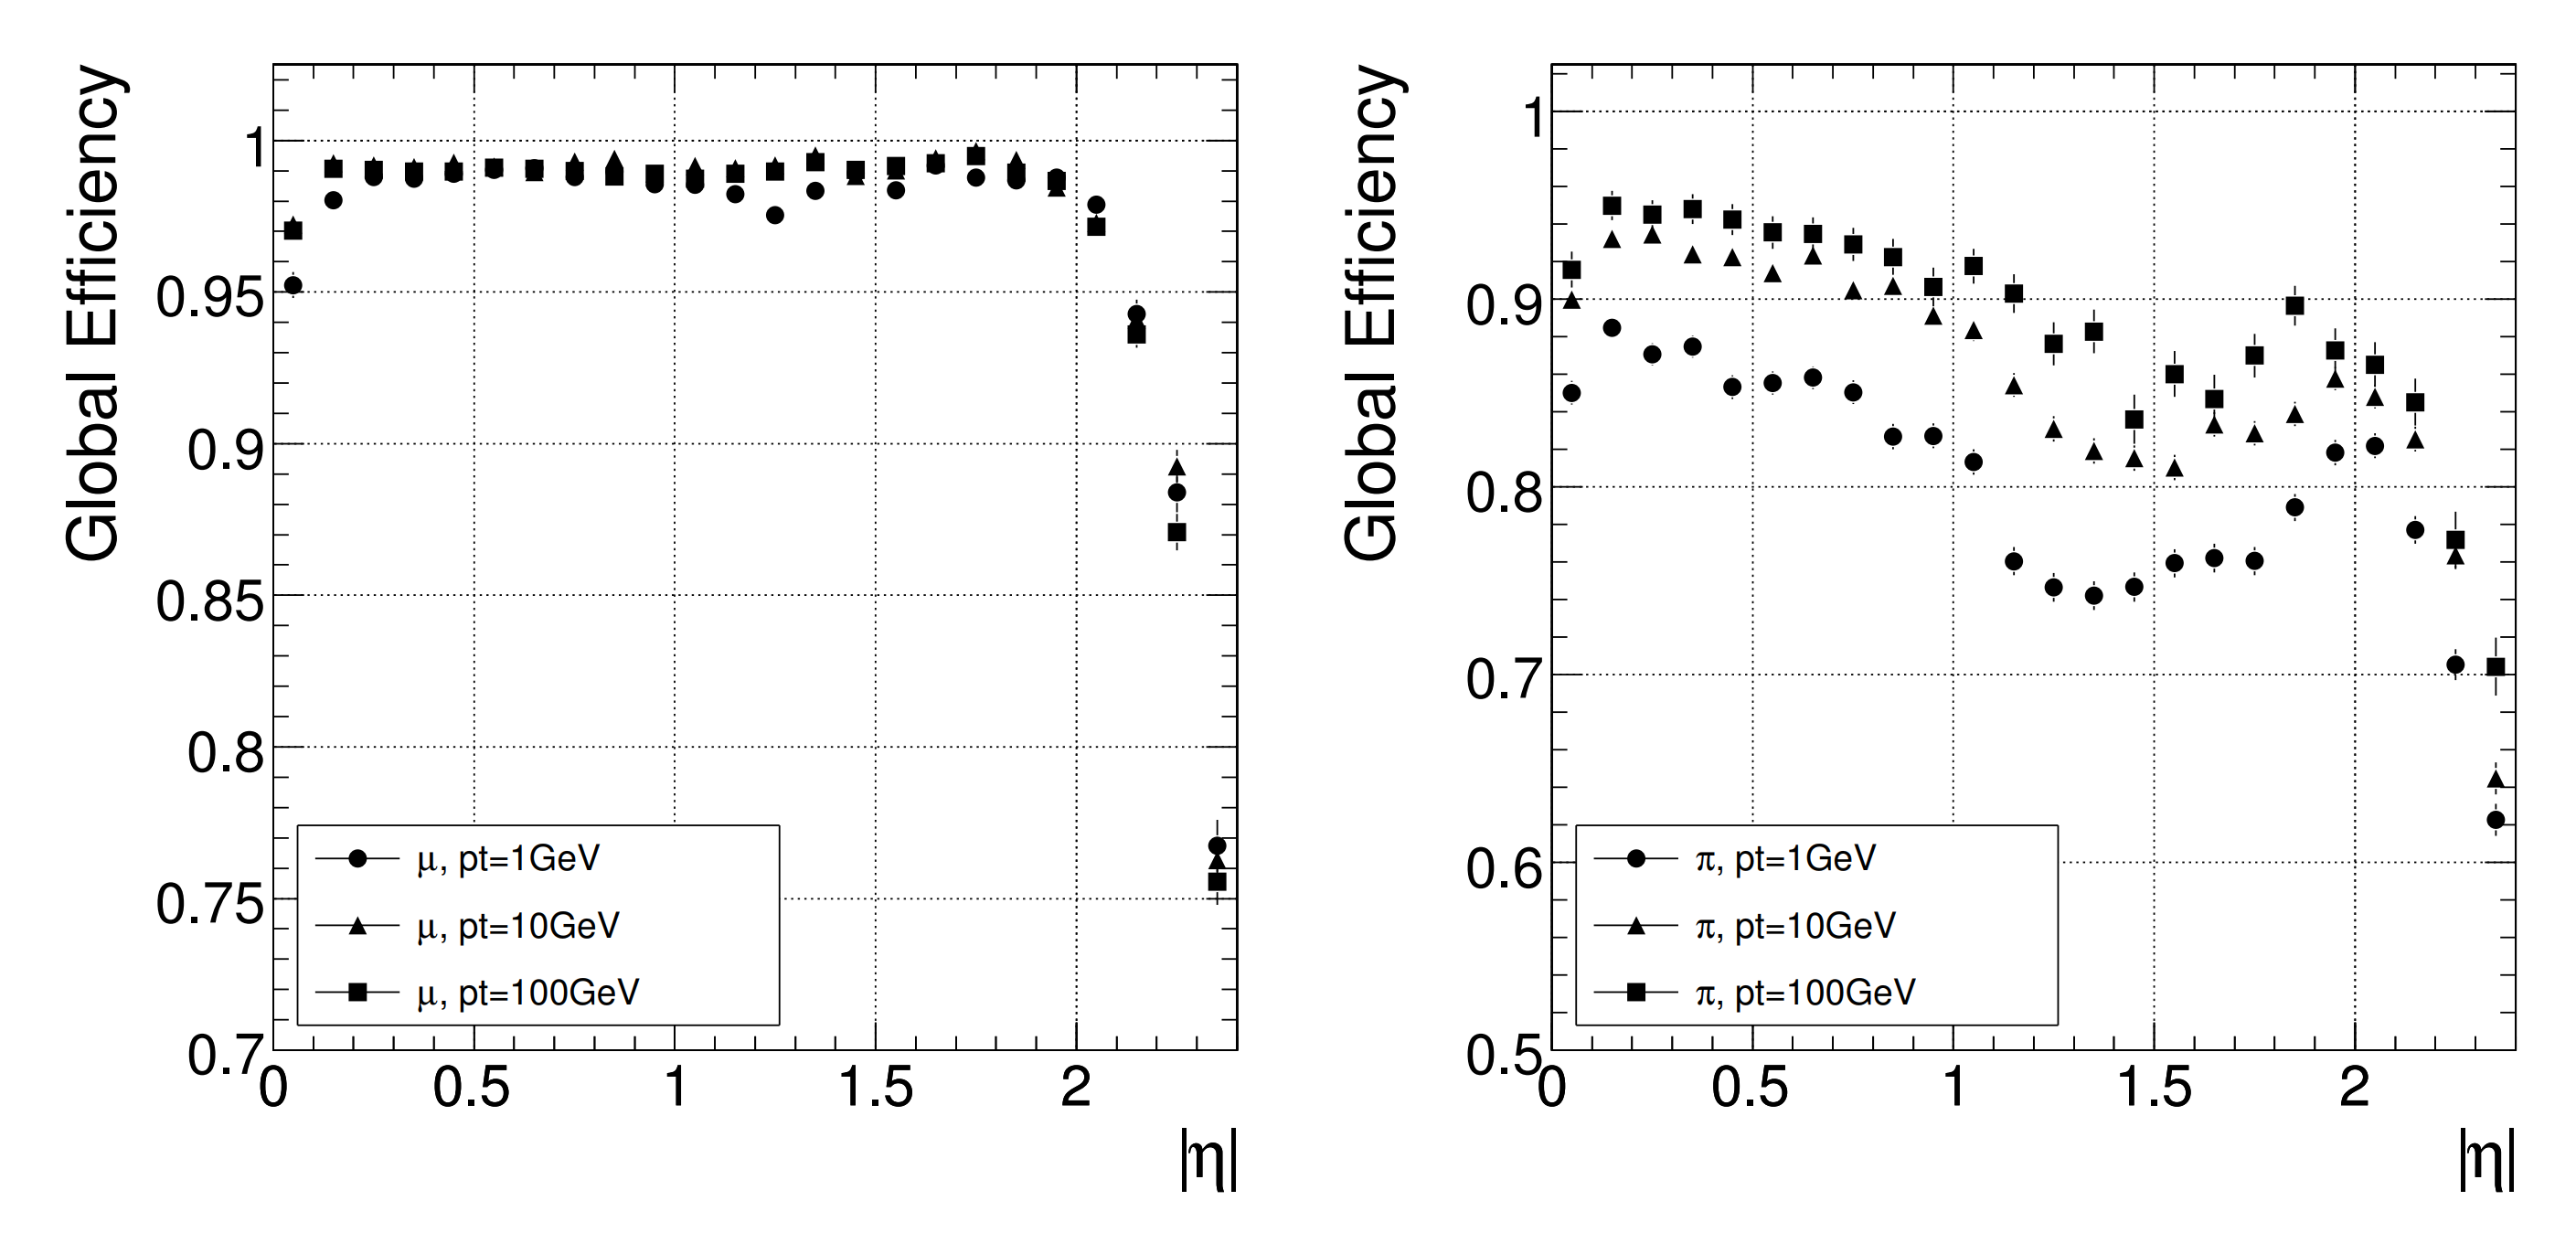
\includegraphics[width=12cm, height=5.5cm]{figs/TrackerEff.png}
\caption{Tracker reconstruction efficiency of muons (on the left) and pions (on the right) in simulation for different pseudorapidities and particle momenta (1, 10 and 100 GeV) \cite{CMSDescription}.}
\label{fig:TrackerEff}
\end{center}
\end{figure}

\subsection{\acf{ECAL}} \label{subsection:ECAL}

The \ac{ECAL} of CMS is a mostly homogeneous detector inside the solenoid but enclosing the tracker system that gives information about the energy of electrons and photons, both able to interact electromagnetically with its crystals.

The \ac{ECAL} can also be divided into several sections: first of all, at pseudorapidities $|\eta| < 1.479$ is found the barrel part of the \ac{ECAL} (EB), made out of 61 200 lead tungstate (PbWO$_4$) crystals, located at a radius of 1.29 meters of the beam pipe. Then, two endcaps, each made out of 7 324 of those crystals, increase the coverage of the detector up to $|\eta| < 3$, as shown in Figure~\ref{fig:CMSECAL}, and the preshower completes the \ac{ECAL}.

\begin{figure}[htbp]
\begin{center}
\includegraphics[width=9.5cm, height=6cm]{figs/CMSEcal.png}
\caption{Schematic representation of the sub-systems of the \ac{CMS} \ac{ECAL} \cite{CMSDescription}.}
\label{fig:CMSECAL}
\end{center}
\end{figure}

Its principle of action is simple and based on electromagnetic showers: when a particle such as an electron or a photon enters the \ac{ECAL}, it will start to interact in different ways, depending on its nature. Photons will mainly produce pairs of electrons and anti-electrons, while the electrons themselves tend to emit additional photons by bremsstrahlung effect. This results in a chain reaction during which the incident particle will give most of its energy to the detector itself, energy measurable using photodetectors and photomultipliers. This effect is known as electromagnetic shower, is represented in Figure~\ref{fig:EMShowers} and is usually characterized using the so-called radiation length $X_0$, the mean distance over which a high-energy particle loses all but 1/e of its energy, then determining the total length of interaction of a particle in the \ac{ECAL}. 

\begin{figure}[htbp]
\begin{center}
\includegraphics[width=7cm, height=6cm]{figs/EMShowers.png}
\caption{Schematic representation of a typical electromagnetic shower and the radiation length $X_0$ concept \cite{CMSDescription}.}
\label{fig:EMShowers}
\end{center}
\end{figure}

The high density, short radiation length and low scintillation decay time (smaller than the bunch spacing of 25ns) of the PbWO$_4$ crystals make them perfect candidates towards a compact \ac{ECAL} in \ac{CMS}. These crystals do have some drawbacks as well, mainly their relative fragility when it comes to radiation, and the dependence on the temperature of their response. Indeed, a cooling system had to be built in order to keep the huge detector under temperature variations lower than 0.1$^\circ$ to avoid eventual fluctuations in the response of the crystals.

These crystals, which had to be grown individually in laboratories, measure 2.2 x 2.2 x 23 cm in the barrel and 3x3x22cm in the endcaps, cover a solid angle equal to ($\Delta \eta$, $\Delta \phi$) = (0.0174, 0.0174), and have therefore a length corresponding to around 26 radiation lengths, more than enough to stop even the most energetic particles. Since the light output of such crystals is quite low (only around 4.5 photoelectrons per MeV of energy), they have to be connected to both avalanche photodiodes and vacuum phototriodes in order to multiply the signal measured. Finally, they have been mounted using a specific installation, slightly tilted with respect to both $\phi$ and $\eta$ in order to remove any possible gap between two adjacent crystals.

The typical energy resolution of the \ac{ECAL} installed at \ac{CMS} is given by Equation~\ref{eq:CMSEcal} \cite{CMSDescription}, accounting for several different effects, such as the stochastic nature of the observed scintillation, the electronics and \ac{PU} noise and the calibration and detector non-uniformity uncertainty.

\begin{equation}
\label{eq:CMSEcal}
\frac{\sigma_E}{E} = \sqrt{\left ( \frac{2.8 \%}{\sqrt{E}} \right)^2 + \left ( \frac{0.12 \%}{E} \right )^2 + (0.30 \%)^2} \sim \frac{3-10\%}{\sqrt{E/\text{GeV}}}
\end{equation}

Finally, a preshower layer has been set up in the fiducial region ($1.653 < |\eta| < 2.6$) of the endcaps, where the angle between the two photons coming from the decay of neutral pions $\pi^0 \rightarrow \gamma \gamma$ is small enough to be misidentified as individual photons. This detector has then been installed in order to reduce the possible misidentification of such events and to help with the identification of electrons against minimum ionizing particles. It is made of a lead layer able to initiate the electromagnetic shower process, followed by two layers of silicon strips for the actual measurement.

\subsection{\acf{HCAL}}\label{subsection:HCAL}

We know that charged hadrons lose energy in a continuous when they traverse matter due to the ionization process and that all the hadrons strongly interact with the nuclei of any given medium. These principles are actually used in order to measure the energy of the hadrons produced by the \ac{LHC} collisions using the \ac{HCAL} sub-system of \ac{CMS}. 

In this case as well, showers of particles due to a chain reaction are expected since the primary hadronic interaction will produce several additional hadrons, themselves interacting even more with the medium while losing energy. This kind of hadronic showers is characterized by the $\lambda$ parameter, the nuclear interaction length, defined as the mean distance between two interactions of relativistic hadrons. The nuclear interaction length $\lambda$ is usually much larger than the radiation length $X_0$, resulting in a \ac{HCAL} typically much larger in size than the \ac{ECAL}. 

A typical \ac{HCAL} setup consists in alternating thick and high-density layers of absorber material, in which the showers can develop, and thin layers of active material used for the actual detection by sampling the energy deposition. This measurement is usually much less precise than the measurement provided by the \ac{ECAL}, mostly since $\pi^0$ decaying into photons can appear in these showers, leading to an electromagnetic component of the shower that cannot be measured, and because around 30\% of the incident energy is usually lost due to nuclear excitation and break-up effects \cite{Thomson}. In this case, the energy resolution can therefore be expressed using Equation~\ref{eq:HCALRes}.

\begin{equation}
\label{eq:HCALRes}
\frac{\sigma_E}{E} > \frac{50\%}{\sqrt{E/\text{GeV}}}
\end{equation}

In \ac{CMS}, the \ac{HCAL}, represented in Figure~\ref{fig:CMSHCAL}, is also divided into a barrel (HB), radially constrained between radii values of 1.77 meters (outer radius of the \ac{ECAL}) and 2.95 meters (inner radius of the solenoid), and two symmetrical forward regions (HF) extending the pseudorapids coverage from $|\eta| = 3$ to $|\eta| = 5.2$ and located at a distance of 11.2 meters to the \ac{PV}. A final part composing the \ac{HCAL} is the so-called \ac{HO}, which has to be put outside of the solenoid in order to increase the amount of shower absorber material of the \ac{HCAL} and therefore the effective nuclear radiation length $\lambda$.

\begin{figure}[htbp]
\begin{center}
\includegraphics[width=11cm, height=8cm]{figs/CMSHCAL.png}
\caption{Schematic representation of the \ac{HCAL} sub-system in \ac{CMS} \cite{CMSDescription}.}
\label{fig:CMSHCAL}
\end{center}
\end{figure}

The \ac{HCAL} barrel uses 36 identical azimuthal wedges as absorber, placed along the beam axis in such a way that the eventual cracks between them is smaller than 2 mm. The total absorber thickness at a $90^{\circ}$ incidence angle is equal to only $5.8 \lambda$, which explains why the \ac{HO} had to be added in order to increase this value to make sure to slow down and completely stop even the most energetic hadrons. The active medium of the HB is made out of 70 000 tiles able to collect the scintillation light, using the wavelength shifting fiber concept to reduce the energy of detected photons and measure the energy of the hadrons. The HF on the other hand are using a Cerenkov-based radiation-hard technology to make the measurements required.

The barrel covers $|\eta|$ regions up to 1.3, while the coverage up to $|\eta| < 5.2$ is given by two endcaps on each side of the detector, placed in such a way to minimize the eventual cracks between the HB and the two HF. Finally, the \ac{HO}, built in order to ensure adequate sampling depth at low pseudorapidity values, actually uses the solenoid itself as additional absorber material, since it is placed a bit outside of this coil. Its shape is constrained by the muon system and the mean fraction of recovered energy from the \ac{HO} has been estimated to be equal to 0.38\% for 10 GeV pions and up to 4.3\% for 300 GeV pions, as shown in Figure~\ref{fig:HOImpact}.

\begin{figure}[htbp]
\begin{center}
\includegraphics[width=15cm, height=4.5cm]{figs/HOImpact.png}
\caption{Distribution of the measured energy scaled to the incident energy for pions with incident energies of 200 GeV at $\eta = 0$ (on the left) and 225 GeV at $\eta = 0.5$ (on the right), with and without the inclusion of the \ac{HO} in the \ac{HCAL} system \cite{CMSDescription}.}
\label{fig:HOImpact}
\end{center}
\end{figure}

\subsection{Solenoid} \label{subsection:Solenoid}

The central piece of \ac{CMS} is its extremely large (12.5 meters of length and 6 meters of diameter) and heavy (220 tons) superconducting solenoid able to produce a 3.8 T magnetic field, storing when active a huge energy of 2.6GJ. It is the largest magnet of its type ever constructed, therefore allowing the tracker, \ac{ECAL} and \ac{HCAL} calorimeters to be placed inside the coil, resulting in a detector that is, overall, quite compact compared to detectors of similar weight.

The magnetic field produced by this coil is extremely useful since it allows to measure quite precisely the charge and the momentum of the different charged particles interacting with the detector just by measuring the curvature of their track, according to the Lorentz Equation~\ref{eq:Lorentz}. This solenoid has been designed to reach a momentum resolution $\Delta p/p \sim 10$\% at $p = 1$ TeV. 

\begin{equation}
\label{eq:Lorentz}
\overrightarrow{F} = \frac{m \overrightarrow{v}^2}{R} =  q \overrightarrow{E} + q \overrightarrow{v} \times \overrightarrow{B} = q \overrightarrow{v} \times \overrightarrow{B}
\end{equation}

The hoop strain, normal stress parallel to the axis of cylindrical symmetry applied throughout this solenoid is quite large ($\epsilon = 130$MPa) compared to the strain applied on other previous detectors and it had to be taken into account during the conception of this magnet. It has then been designed in such a way that a large fraction of the \ac{CMS} coil has a structural function, dividing the strain between the layers of the magnet and the support of the coil itself ($\sim 30$\%). At the end, the conductor of this solenoid, made from a Rutherford-type cable combined with aluminum, is mechanically reinforced with an aluminum alloy.

The coil of the magnet is then completed with a huge steel yoke return system, as seen in Figure~\ref{fig:CMSMagnet}, made out of 6 endcap disks and 5 barrel wheels, weighting in total more than 12 000 tons and therefore accounting for most of the weight of \ac{CMS}. This system is composed of many steel blocks up to 620 mm thick combined and actually also serves as the absorber plates of the \ac{HO} and muon detection system that will be described in the next section. %A precise alignement system is then needed in order to hermetically close the detector and to make sure that the magnet is working efficiently each time the detector needs to be opened, usually once a year and during the \acfp{LS}. 

\begin{figure}[htbp]
\begin{center}
\includegraphics[width=8cm, height=6cm]{figs/CMSMagnet.jpg}
\caption{Picture of the solenoid system of \ac{CMS} being setup in the assembly hall.}
\label{fig:CMSMagnet}
\end{center}
\end{figure}

Finally, a two pumping stations system has been put in place in order to setup a vacuum as strong as possible inside the 40 m$^3$ volume of the coil cryostat and an helium refrigeration plant has been installed near the site of the detector, able to cool down the solenoid up to 4.5 K, giving a 2 K security margin with respect to the critical field of the superconducting coil. All these systems were extensively tested on the surface during the summer of 2006, before lowering down the complete solenoid in the experimental cavern where it now stands.

\subsection{Muon system} \label{subsection:Muon}

The muon detection is extremely useful since many interesting processes are expected to produce such particles. Their detection and the correct measurement of their main properties such as their position and momentum is therefore crucial in most of the analyses performed. Detecting muons is at the end of the day quite easy, as we will see, and the data extracted from them is usually more reliable than the one obtained from electrons since muons are less likely to be affected by the inner parts of the detector, such as the tracker, because of their low interaction cross section.

The muon system of \ac{CMS} is actually made out of three different gaseous sub-subsystems combined in order to perform a reconstruction as precise as possible of such particles over the the entire kinematic range of the \ac{LHC}. These different muon chambers systems do share some characteristics: they mostly have to be distributed over a cylindrical area, because of the geometrical shape of the inner systems of \ac{CMS} and they have to be reliable and cheap, since they cover a total area corresponding to more than 25 000 m$^2$.

\begin{figure}[htbp]
\begin{center}
\includegraphics[width=12cm, height=8cm]{figs/CMSMuons.png}
\caption{Geometrical repartition along the z-axis of the different muons chambers in \ac{CMS} \cite{CMSMuons}.}
\label{fig:CMSMuons}
\end{center}
\end{figure}

Each category of muon chambers is typically used in a different pseudorapidity area, as shown in Figure~\ref{fig:CMSMuons}, in order to form a muon system as hermetic as possible.

\subsubsection*{\acfp{DT}}

First of all, in the barrel region, where the flux of muons is low and where the magnetic field is mostly uniform and low as well, the \textbf{\acp{DT}} have been installed. This system covers the $|\eta| < 1.2$ area and has been divided into 4 different layers, each containing a number of stations optimized in order to provide a full coverage of the $\theta$ angles, a good efficiency for the muon hits reconstruction into a single track and a good rejection of eventual background hits. This distribution of the \acp{DT} is represented in Figure~\ref{fig:CMSDT}.

\begin{figure}[htbp]
\begin{center}
\includegraphics[width=12cm, height=10cm]{figs/CMSDT.png}
\caption{Lateral geometrical division of the different \ac{DT} chambers in one of the 5 wheels of \ac{CMS} \cite{CMSDescription}.}
\label{fig:CMSDT}
\end{center}
\end{figure}

The \ac{DT} system is made out of 172 000 sensitive wires able to collect the residuals charges left by the ionization tracks of muons through the 250 chambers installed. The system has been set up in such a way that the maximal drift of any charge is lower than 21mm, corresponding to a drift time of 380 ns in the gaseous chambers made out of 85\% of Ar and 15\% of CO$_2$, a value small enough to produce negligible occupancy in the different wires and to avoid the need of multi-hits electronics. Redundancy of the \acp{DT} provided by the installation of multiple layers is extremely important, mainly to reduce the backgrounds coming from eventual neutrons or photons, whose rate is actually much larger than the one obtained from prompt muons.

\subsubsection*{\acfp{CSC}}

In the two endcap regions, where the muon rates and the background levels are much larger and where the magnetic field is large and non-uniform, a different system had to be installed. First of all, the \textbf{\acp{CSC}}, multi-wire proportional chambers providing a fast response while being resistant to the radiation, are able to identify muons in a $0.9 < |\eta| < 2.4$ region (in the $0.9 < |\eta| < 1.2$ region, muons cross both \acp{DT} and \acp{CSC} while in the $1.2 < |\eta| < 2.4$ area, muons typically cross between 3 and 4 \acp{CSC} only). 

This sub-system is made out of 540 different chambers in total, all perpendicular to the beam pipe. The sensitive plates of this sub-system are made out of 2 million wires, cover about 5000 m$^2$ and the total gas volume included in such chambers is equal to about 50 m$^3$.

\subsubsection*{\acfp{RPC}}

Finally, some \textbf{\acp{RPC}} have been added to the barrel and to the endcap regions in order to cope with the uncertainty associated with the eventual background rates and with the (in)ability of the previous muon
system to identify unequivocally the correct bunch crossing when the \ac{LHC} is running at full luminosity. Indeed, the time resolution of the \acp{DT} of 380 ns is way larger than the bunch spacing in the \ac{LHC}, while a \ac{RPC} is capable
of tagging an ionizing event in less than 25ns, making it an ideal candidate to trigger the event.

The \acp{RPC} are double-gap chambers operated in avalanche mode to ensure good operation at high rates and they are able to produce a fast response with good time resolution, even though its position resolution is worse than the one obtained with \acp{DT} or \acp{CSC}. The \acp{RPC} are also useful in the sense that they can help to resolve ambiguities when attempting to construct tracks from multiple hits in a chamber. 

Finally, the different features of the three muon sub-systems used by the \ac{CMS} detector are summarized in Table~\ref{table:CMSMuonsSystems}.

\begin{table}[h!]
\begin{center}
\begin{tabular}{ c|c|c|c } 
 \hline
 Muon sub-system & \ac{DT} & \ac{CSC} & \ac{RPC} \\
 \hline
 $|\eta|$ coverage & 0.0-1.2 & 0.9-2.4 & 0.0-1.9 \\
 Stations & 4 & 4 & 4 \\
 Chambers & 250 & 540 & \makecell{\vspace{-10pt} \\ 480 (barrel) \\ 576 (endcaps)} \\
 Readout channels & 172 000 & \makecell{\vspace{-10pt} \\ 266 112 (strips) \\ 210 816 (anode channels)} & \makecell{\vspace{-10pt} \\ 68 136 (barrel) \\ 55 296 (endcaps)} \\
 Spatial resolution & 80-120 $\mu$m & 40-150 $\mu$m & 0.8-1.2 cm \\
 Average efficiency (13 TeV) & 97.1\% & $97.4$\% & \makecell{\vspace{-10pt} \\ 94.2\% (barrel) \\ 96.4\% (endcaps)} \\ 
 \hline
\end{tabular}
\caption{Comparison of the three main sub-systems currently used by \ac{CMS} in order to identify and measure muons \cite{MuonSystemsEff}.}
\label{table:CMSMuonsSystems}
\end{center}
\end{table}

Another advantage of the muon system such as the one built in \ac{CMS} is that it can also directly be used by the trigger system, which will be described in Section~\ref{subsection:Trigger}, independently of the rest of the detector and in addition of being able to detect, identify and measure several properties of muons crossing it.

The muon reconstruction efficiency obtained by the muon system strongly depends on the pseudorapidity value of the muon considered, along with its transverse momentum, as shown in Figure~\ref{fig:MuonRecoEff}. In this figure, we can also see that several different kinds of muons can be defined, such as the \textbf{standalone muons}, defined using only the data coming from the muon system and the \textbf{global muons}, defined using both the information coming from the muon system and the tracker. This distinction will be detailed when discussing about the muons reconstruction in Section~\ref{subsection:Muons}). %Cross-checks between the different systems of \ac{CMS} can therefore be performed, as will be described in Chapter~\ref{chapter:Reco}.

\begin{figure}[htbp]
\begin{center}
\includegraphics[width=14cm, height=6cm]{figs/muonRecoEff.png}
\caption{Muon reconstruction efficiency with different $p_T$ and $\eta$ values, considering only the muon system (on the left), and the combined information from the muon system and the tracker (on the right) \cite{CMSDescription}.}
\label{fig:MuonRecoEff}
\end{center}
\end{figure}

Taking advantage of the \ac{LS}2, a new muon system is currently being installed in the experimental cavern: the so-called \textbf{\acfp{GEM}}, placed in the endcaps, where the radiation and event rates are the highest. This new subdetector will provide additional redundancy and measurement points to the current system, therefore allowing a better muon track identification and reconstruction and a wider coverage in the very forward region. 

The first 144 chambers of the \ac{GEM} sub-system, filled with a mixture of Ar and CO$_2$ and where the primary ionization due to incident muon is expected to happen, are currently being installed in the first disk of both endcaps (cf. Figure~\ref{fig:CMSGEM}), while the rest will be set up during the next \ac{LS} expected in 2024, before the phase II of operation of the \ac{LHC}.

\begin{figure}[htbp]
\begin{center}
\includegraphics[width=12cm, height=7cm]{figs/CMSGEM.png}
\caption{Location of the new \ac{GEM} muon subsystem currently being installed in the very-forward region of \ac{CMS} \cite{CMSDescription}.}
\label{fig:CMSGEM}
\end{center}
\end{figure}

\subsection{Trigger system} \label{subsection:Trigger}

The \ac{CMS} experiment faces a data acquisition limitation since the collision rate delivered by the \ac{LHC} (one bunch crossing each 25ns, leading to an impressive rate of collisions of 40 MHz) is much larger than the data acquisition rate currently achievable by nowadays electronics (around 1kHz only, more or less equivalent to 1Gb of data per second). It is therefore impossible to store and process all the collisions provided by the \ac{LHC}; instead, a selection needs to be made in order to select and record only the most interesting events.

A system, called the trigger system, has therefore been put in place in order to select extremely quickly 1 kHz of interesting events out the 40 MHz. This system is based on two different levels: first of all, the \ac{L1}, a hardware set of electronics selecting around 100 kHz of data, followed by the \ac{HLT}, a software layer improving the selection even more.% Let's now give a bit more details about these two levels of trigger.

\subsubsection*{\acf{L1}}

The \ac{L1} is the first level of trigger \cite{L1}, based directly on hardware. In order to maximize its efficiency, it is mostly implemented in different subsystems of the detector (on the calorimeters and muons system) and in the service cavern, just next to the detector, so that the electric signals do not have to travel large distances, therefore saving a few precious nanoseconds of decision time. 

The L1 trigger, whose architecture is represented in Figure~\ref{fig:L1Trigg}, has local, regional and global components. First of all, the local triggers, also referred to the \ac{TPG}, are using the energy deposits measured in the calorimeter and the track segments or hit patterns in the muon chambers. Then, regional triggers combine this information and use pattern logic to determine ranked and sorted trigger objects
such as electron or muon candidates in limited spatial regions. The rank is typically determined as a function of energy or momentum and quality, which reflects the level of confidence attributed to the L1 parameter measurements, based on detailed knowledge of the detectors and trigger electronics
and on the amount of information available. Finally, the global calorimeter and muon triggers combine this local information to determine the highest-rank calorimeter and muon objects across the entire experiment and transfer them to the the top entity of the L1 hierarchy, the global trigger. This level is in charge of taking the final decision on whether to keep or reject the event, and eventually passes it to the \ac{HLT}.

\begin{figure}[htbp]
\begin{center}
\includegraphics[width=9cm, height=6cm]{figs/L1Trigg.png}
\caption{Architecture of the \ac{L1} trigger of \ac{CMS} \cite{CMSDescription}.}
\label{fig:L1Trigg}
\end{center}
\end{figure}

This trigger gets new data each 25ns and today's electronics is not fast enough in order to deal with such a massive input of data, so an ingenious systems of buffers had to be put in place in order to put in line several events before analyzing all of them at once, using only basic segmented data provided by the detector.

\subsubsection*{\acf{HLT}}

On the other hand, the \ac{HLT} \cite{HLT} does get access to the complete read-out data of the detector, since the rate has already been strongly reduced by the \ac{L1} Trigger, allowing it to perform complete calculations such as the ones that will be later performed offline. Since this is a software based layer and the decision time is not as critic, it runs on a farm of computers on the surface and is in constant evolution, getting constantly improvements and updates in order to select and reconstruct in a better and more efficient way interesting data from the collisions.

The \ac{HLT} uses the so-called \textbf{trigger paths} in order to select specific particle topologies in the collisions. This selection imposes some thresholds on key quantities of the different objects, such as their transverse momentum $p_T$, to avoid passing the bandwidth limit of 1kHz. In some cases, not all the events of a given category can be collected and only a fraction of them are therefore recorded. Trigger paths designed to behave like this are called pre-scaled trigger paths.

\subsection{\acf{DAQ}} \label{subsection:DAQ}

In summary, the CMS \ac{DAQ}, whose global architecture is represented in Figure~\ref{fig:CMSDAQ}, has been designed to collect and analyze the data information at the nominal collision rate of 40MHz and is fed directly from the \ac{L1} trigger. This means that it has to be able to read a flux of data of the order of 100kHz ($\sim 100$Gb/s) coming from approximately 650 different sources at once, while providing enough computing power for the \ac{HLT} to be able to reduce this rate by a factor $\sim 100$, while keeping some resources available for other tasks.

\begin{figure}[htbp]
\begin{center}
\includegraphics[width=9cm, height=4.5cm]{figs/CMSDAQ.png}
\caption{Architecture of the \ac{CMS} \ac{DAQ} system \cite{CMSDescription}.}
\label{fig:CMSDAQ}
\end{center}
\end{figure}

The \ac{DAQ} is indeed also in charge of performing additional tasks, such as the generation of the \ac{DQM} information resulting
from online event processing in the \ac{HLT}, the transfer of the data from local storage at the \ac{CMS} site to mass storage in the \ac{CERN} data center at the Meyrin site and the operation of the \ac{DCS} system, ensuring the correct operation of the detector and a high quality data taking at all times. %The \ac{DAQ} is therefore an essential part of the detector.

\section{\acs{CMS} main goals}

At the end of the day, the \ac{CMS} detector has been built in order to meet the goals of the \ac{LHC} physics program, which have been summarized in \cite{CMSDescription} as:

\begin{itemize}
\item Good muon identification and momentum resolution over a wide range of momenta and angles, good dimuon mass resolution ($\sim 1$\% at 100 GeV), and the ability to determine unambiguously the charge of muons with momentum $p <$ 1 TeV.
\item Good charged-particle momentum resolution and reconstruction efficiency in the inner tracker. Efficient triggering and offline tagging of taus and b-jets, requiring pixel detectors close to the interaction region.
\item Good electromagnetic energy resolution, good diphoton and dielectron mass resolution ($\sim 1$\% at 100 GeV), wide geometric coverage, $\pi^0$ rejection, and efficient photon and lepton isolation at high luminosities.
\item Good missing-transverse-energy and dijet-mass resolution, requiring hadron calorimeters with a large hermetic geometric coverage and with fine lateral segmentation.
\end{itemize}




























\chapter{Event reconstruction} \label{chapter:Reco}

The \ac{CMS} detector is made out of different layers, each able to convert the interaction of the particle into electronic signals that can be measured and stored. However, these collected electronic signals are made out of raw information coming from different kinds of subsystems and an algorithmic strategy then needs to be put in place in order to read and combine them to extract some useful data, such as the number of particles produced by the collision along with their energy, charge and direction. Producing this kind of data is essential for all the offline analyses which usually rely on these high-level physics objects to make precision measurements or search for new physics. 

The algorithm able to combine this raw data and to compute and produce useful kinematic variables and physical objects (such as leptons and jets) is the so-called \acf{PF} algorithm \cite{PF}, which will be first of all described in Section~\ref{section:PF}. Then, a particular focus will be given to the definition and reconstruction of different objects of our particular analysis, such as electrons and muons (Section~\ref{section:RecoLep}), jets (Section~\ref{section:RecoJet}), the \ac{MET} (Section~\ref{section:RecoMET}) and the top reconstruction (Section~\ref{section:RecoTop}) of the different $pp$ collisions recorded.

\section{Particle Flow algorithm} \label{section:PF}

The \ac{PF} is an algorithm aiming to combine in the best way possible all the information coming from the different parts of the \ac{CMS} detector (mostly, tracks and clusters of energy) in order to identify and reconstruct the hundreds of new particles produced by each $pp$ collision provided by the \ac{LHC}. This reconstruction can be divided into two main steps: first of all, the data coming from the different subsystems of the detector is read in order to identify and measure the properties of some basic stable objects, such as leptons, photos and hadrons. Then, more complex calculations are performed to identify eventual unstable particles, jets from the hadronization of quarks and gluons, and to compute complex variables such as the leptons isolation and the \ac{MET}.

The most basic elements used by this algorithm for the reconstruction of high-level physics objects are the hits left by charged particles in the tracker and in the muon chambers, and the clusters of energy left in the two calorimeters. For this algorithm to be as efficient as possible, the detector has been carefully designed, as described in Chapter~\ref{chapter:Device}: a magnetic field as intense as possible and a small calorimeter granularity are indeed crucial in order to separate efficiently charged and neutral particles, and the tracker was designed to be as efficient and small as possible to have the smallest material budget possible in front of the calorimeters. The muon system has been carefully designed as well and, in general, the whole detector is obviously as hermetic as possible.

The way the different particles produced in each collision are identified is quite easy to summarize and is represented in Figure~\ref{fig:CMSIdentify}. Basically, the different kinds of particles produced are going to interact with different parts of the detector and combining the information given by the tracker and the rest of the subsystems then allows to unequivocally identify each particle. This is usually done in a specific order to make this process as efficient as possible:

\begin{enumerate}
\item First of all, the most energetic \textbf{\acf{PV}} is identified by taking into account the \ac{PU} and by assigning the different tracks to the different $pp$ collisions happening during a single bunch-crossing. 

All the tracks originating from less energetic \ac{PV} or from a secondary vertex of interaction are typically ignored and the corresponding hits in the tracker left by such particles can therefore be ignored later on, leaving less hits available for the clustering algorithm later on, allowing for a more efficient reconstruction of the following objects.
\item Then, \textbf{muons} are the easiest particles to identify since they are at first order the only particles leaving many hits in the muon chambers placed on the outside of the detector. Depending on the version of the algorithm used, each muon identified can be associated to its track in the tracker, where all the hits matching a muon can therefore be subsequently ignored to simplify the following reconstruction steps.
\item \textbf{Electrons} do have a charge, so they are visible by the tracker, and can interact electromagnetically with the \ac{ECAL}, where they are going to produce an electromagnetic shower. Identifying electrons is a bit more challenging than muons because of their associated bremsstrahlung emission of photons that need to be attached to the original electrons to measure efficienctly their complete energy and avoid any double counting. All the tracker hits corresponding to electrons are also ignored for the rest of the reconstruction after identification.
\item \textbf{Charged hadrons} also leave hits in the tracker and some energy deposits in the \ac{ECAL}, but mostly in the \ac{HCAL}, so they are easy to identify as well as a fourth step, using the last hits available in the tracker.
\item \textbf{Photons} are on the other hand neutral particles, so they do not leave any hits in the tracker. They then appear as some energy deposits in the \ac{ECAL} for which no corresponding tracker track can be associated.
\item Finally, \textbf{neutral hadrons} can be identified as particles leaving some energy mostly in the \ac{HCAL} for which no corresponding tracker track has been found as well.
\end{enumerate}

\begin{figure}[htbp]
\begin{center}
\includegraphics[width=13cm, height=8cm]{figs/CMSIdentify.png}
\caption{Transverse section of \ac{CMS} showing the different interactions expected by different kinds of particles in the detector.}
\label{fig:CMSIdentify}
\end{center}
\end{figure}

We will now study in more detail the reconstruction method applied in order to reconstruct the main objects of this analysis, i.e. the leptons, jets, \ac{MET} and bottom/top quarks.

\section{Primary vertex definition} \label{section:PVDef}

Different kinds of vertices originating from a single $pp$ collision can usually be defined, as shown in Figure~\ref{fig:LHCPU}: the \textbf{\ac{PU} vertices}, corresponding to the different simultaneous collisions of a single bunch-crossing of the \ac{LHC} or eventual remnants coming from a previous collision (the out-of-time \ac{PU}) the \textbf{\ac{PV}}, usually assumed to be the most energetic \ac{PU} vertex and the only vertex considered in most of the physics analyses, and the \textbf{secondary vertices}, due to the eventual presence of hadrons living long enough to travel a significant distance in the detector, decay chains or jets. 

The first task of the \ac{PF} algorithm is to identify all these vertices. This is done by considering all the tracker hits observed, by clustering them together and by performing fits to determine the likelihood these tracks originating from a common vertex. The reconstructed vertex with the largest $p_T^2$ summed over all the physics objects of the event is then assumed to be the \ac{PV}, as it is considered to be the origin of the collision that actually fired the trigger, from which many different tracks are emitted.

\begin{figure}[htbp]
\begin{center}
\includegraphics[width=7.5cm, height=4cm]{figs/LHCPU.png}
\caption{Different kinds of vertices typically observed in a $pp$ collision in the \ac{LHC}.}
\label{fig:LHCPU}
\end{center}
\end{figure}

\section{Leptons reconstruction} \label{section:RecoLep}

Different kinds of leptons are typically produced by a $pp$ collision. The muons and the electrons and their respective anti-particles can be quite easily identified, mainly because their lifetime and velocity is high enough, meaning that they are not expected to decay inside the \ac{CMS} detector, so they can be directly identified. Taus on the other hand are a bit trickier to deal with because they usually decay inside of the beam pipe itself, $\sim 35\%$ of the time to electrons and muons and $\sim 65\%$ of the time to hadrons. However, since our analysis does not consider taus directly but only the leptons originating from their decays, the details of their reconstruction will not be explained in this section.

\subsection{Muons} \label{subsection:Muons}

Muons are the first leptons to be reconstructed by the \ac{PF} algorithm since, by design and at first order, they are the only particles expected to reach the muon chambers, resulting in an easier and more efficient identification. 

The typical signature of a muon consists of several hits in the silicon tracker forming a track associated with several hits in the muon chambers, electronic signals coming from the wires and strips of these chambers due to the gas ionization induced by the passage of these charged particles. Muons only deposit a negligible amount of energy within the two calorimeters since their interaction cross section is quite low for their full range of energies, going from a few hundreds MeV up to a few TeV.

The data coming from the different subsystems of \ac{CMS} are then combined and fed into three different \ac{PF} algorithms, able to reconstruct different kinds of muons \cite{MuonSystemsEff}.

\subsubsection*{Standalone muons}
The standalone muons are muons reconstructed using only the hits observed in the muon system without trying to relate this data to the tracker hits. Basically, the \ac{PF} algorithm looks in this case at the eventual hits left in the \acp{DT}, \acp{CSC} and \acp{RPC} and tries to reconstruct a vector of trajectory in each case using a \ac{KF} \cite{KF}. The segments obtained are then combined in the best statistical possible way in order to form a candidate track for each muon of the event, by extrapolating the innermost vectors obtained to the next chamber and by comparing it with the local track segment; the trajectory parameters are then updated and the process continues until reaching the outermost chamber. Finally, this complete process is repeated in the reverse order, from the outside chambers to the inside, to estimate the innermost track parameters as well.

It is important to note that cosmic rays reaching the Earth every day are an important source of contamination, since we estimate that around 10.000 muons per $m^2$ and per minute coming from such processes can be observed at the sea level. Putting the detector underground removes part of this contamination but, to further limit the possibility of misidentification due to showering of cosmic rays, the tracks need to pass some quality criteria: for example, checking the extrapolation of the trajectory to the point of closest approach to the beam line allows to reduce this contamination. Additionally, at least two hits need to be measured for the fit to be performed, one of them coming from either the \acp{DT} or \acp{CSC}, in order to remove fake segments contamination due to combinatorics.

In any case, candidates reconstructed as standalone muons typically have a worse momentum reconstruction and are more sensitive to cosmic muons contamination.  

\subsubsection*{Tracker muons}
The algorithm able to reconstruct the so-called tracker muons on the other hand is able to propagate tracks identified in the inner silicon tracker (having a momentum $p > 2.5$ GeV and $p_T > 0.5$ GeV) to the muon system itself in order to try and find corresponding segments in the different muon chambers (these tracks are therefore said to be built \textit{inside-out}). An extrapolated track and a segment are only matched if the difference between their positions in the $x$ coordinate is smaller than 3~cm or if the pull, the ratio of this distance to its uncertainty, is smaller than 4.

These muons are particularly efficient for less instrumented regions of the detector and for the low $p_T$ end of the energy spectrum but they are also quite contaminated with fake muon tracks, since a single hit in any of the muon chambers is enough for the candidate to be considered a valid tracker muon, even though hadron shower remnants can for example quite easily reach the innermost muon station. The momentum assigned to such muons is the same as the one measured by the silicon tracker track itself.

\subsubsection*{Global muons}
Finally, these muons are built \textit{outside-in} since they are obtained by matching standalone muon tracks with independently reconstructed tracks coming from the tracker itself (of course, in order to avoid any double counting, global muons and tracker muons that share the same tracker track are actually merged into a single candidate). 

This category of muons presents the advantage of being less sensitive to the muon misidentification rate than tracker muons since it uses the information from more than one muon chamber. The $p_T$ measurement in this case is also improved (especially for $p_T > 200$ GeV) by exploiting the information from both the inner tracker and the muon system, while at low momentum, the best momentum resolution for muons is obtained from the inner silicon tracker directly.

Using this strategy, about 99\% of the muons produced within the geometrical acceptance of the muon system are reconstructed either as global or tracker muons, as seen in Figure~\ref{fig:MuonEff2}.

\begin{figure}[htbp]
\begin{center}
\includegraphics[width=13cm, height=6cm]{figs/MuonEff.png}
\caption{Muon $p_T$ resolution obtained in simulation in the barrel (on the left) and endcap (on the right) for different muon reconstruction algorithms \cite{Quarkonium}.}
\label{fig:MuonEff2}
\end{center}
\end{figure}

Once reconstructed, candidates are required to pass some selection criteria and are then fed to the actual \ac{PF} algorithm itself to start the global reconstruction of the event. This selection consists mainly in applying identification and isolation (evaluated relative to its $p_T$ by summing up the energy in geometrical cones of radius $\Delta R = \sqrt{(\Delta \phi)^2 + (\Delta \eta)^2}$ surrounding the muon in the ($\eta, \phi$) plane, as shown in Figure~\ref{fig:IsoCone}) criteria in order to enhance the purity of the reconstructed prompt muons (muons directly originating from the main collision taking place in the event) by rejecting muons coming from the decay of heavy flavour quarks, typically surrounded by a large amount of hadronic activity. The calculation of the lepton isolation is typically performed considering only the \ac{PV} since higher levels of \ac{PU} are expected to bias this measurement by increasing the hadronic activity.

\begin{figure}[htbp]
\begin{center}
\includegraphics[width=7cm, height=6.5cm]{figs/IsoCone.png}
\caption{Lepton isolation cone typically used to enhance the prompt leptons purity.}
\label{fig:IsoCone}
\end{center}
\end{figure}

Different identification \acfp{WP} can then be defined for the offline analyses, from veto to tight, in order to reject more or less contamination from misidentified leptons, bearing in mind that a tighter selection is cleaner, but less efficient: the loose and tight \ac{WP} have then been defined in order to respectively achieve 95\% and 98\% efficiencies, respectively. These efficiencies are tuned using simulated $Z \rightarrow \mu^+ \mu^-$ events with a $p_T > 20$ GeV, while the efficiency to reject muons in jets is done using simulated QCD and $W$+jets processes \cite{MuonSystemsEff}.

Our particular muon definition is based on the tight \ac{WP} provided centrally by the muon \ac{POG}, but has been slightly modified and made more robust against non-prompt leptons, according to the selection detailed in Chapter~\ref{chapter:Selection}.

\subsection{Electrons} \label{subsection:Electrons}

Electrons and positrons are reconstructed by combining the tracker tracks and the several clusters of energy deposited in the \ac{ECAL} by the electromagnetic showers appearing due to the interaction between the electron and the crystals composing this subdetector. 

It is usually a bit harder to reconstruct electrons than muons mainly because electrons do interact much more with the tracker and this interaction therefore needs to be modeled to understand the exact behaviour of such particles: it is for example responsible for the emission of secondary bremsstrahlung photons crashing into the \ac{ECAL} but not coming from the \ac{PV}. In fact, it is estimated that in \ac{CMS} between 33\% and 86\% of the energy of an electron is actually radiated before it reaches the \ac{ECAL}, depending mostly on its pseudorapidity \cite{EleReco}. In order to measure precisely the energy of an electron, all the photons emitted by bremsstrahlung before reaching the \ac{ECAL} (usually, along the $\phi$ plane because of the deviation implied by the solenoid) then need to be collected as well and associated to the correct electron of the event.

The actual \ac{PF} reconstruction of electrons is performed in different steps:

\begin{enumerate}
\item A \textbf{clustering algorithm} is first of all defining the so-called \textbf{\acf{SC}}. Its goal is to reconstruct the particle showers individually by identifying a seed crystal for the cluster, defined as the crystal collecting the most energy, since the energy deposited in the \ac{ECAL} is usually spread into several different crystals because of the electromagnetic shower effect discussed in Section~\ref{subsection:ECAL} and because of the bremsstrahlung emission of photons due to the interaction with the tracker. The algorithm therefore searches for eventual crystals around this seed whose energy detected would be superior to 2$\sigma$ of the electronic noise and matching some quality criteria ($E_{\text{seed}} > 230$ MeV in the barrel, $E_{\text{seed}} > 600$ MeV and $E_{\text{seed}}^T > 150$ MeV in the endcaps). 

The excited contiguous crystals found are then grouped into clusters, themselves considered candidates for the final global cluster, the \ac{SC}, if their energy is higher than another given threshold ($E_{\text{cluster}} > 350$ MeV in the barrel, $E_{\text{cluster}}^T > 1$ GeV in the endcaps) \cite{EleReco}. The \ac{SC} energy is then given by the sum of the energies of all its constituent clusters, while its position is calculated as the energy-weighted mean position of the different clusters.

\item Once the \ac{SC} is identified, \textbf{electron tracker tracks} are reconstructed using a procedure a bit different than the usual \ac{KF} reconstruction method for all the tracks of the silicon tracker \cite{KF} because of the large radiative
losses for electrons in the tracker material. 

This reconstruction is known to be very time consuming, so a good identification of potential electron seeds has to be performed as the method efficiency greatly relies on this first identification. Two different strategies can be used to perform this seeding (even though the electron seeds found using the two algorithms are usually combined afterwards): 

\begin{itemize}
\item The \textbf{\ac{ECAL}-based seeding} relies on the information obtained for the \ac{SC} energy and position in order to estimate the electron trajectory to find compatible hits in the tracker. This can be done knowing that the electron is moving according to an helix in the magnetic field of the detector. This seeding is mostly optimized for isolated electrons
in the $p_T$ range relevant for the Z and W decays.
\item The other way to proceed is the \textbf{tracker-based seeding}, based on tracks reconstructed using the usual \ac{KF} algorithm and looking for matches within the possible reconstructed \ac{SC}. This seeding is mostly suitable for low $p_T$ electrons and also performs quite well with electrons inside jets.
\end{itemize}

Once the seeds have been identified, the identification of tracks can begin. First of all, the gathering of compatible hits from the different seeds is done using using a dedicated modeling of the electron energy loss and a combinatorial \ac{KF} algorithm allowing to construct possible tracks when compatible hits are found. The compatibility matching between the predicted and found hits is usually chosen to be quite loose in order to maintain a good efficiency even in case of bremsstrahlung emission.

Finally, once the hits are collected, a \ac{GSF} fit is performed to estimate the different track parameters by reconstructing the layer-to-layer propagation of electrons in the tracker. A mix of Gaussian distributions is used in this case to approximate the loss in each layer, associating a different weight and $\chi^2$ penalty to each distribution, depending for example on the number of missing hits. This fit is also able to take into account sudden changes in the curvature radius caused by an eventual bremsstrahlung photon emission.

\item The final step consists in identifying the clusters left in the \ac{ECAL} by the photons emitted by extrapolation of the \ac{GSF} track and in \textbf{merging this \ac{GSF} track and the \ac{ECAL} \acp{SC}} previously built. This step is also designed to preserve the highest efficiency possible while keeping the misidentification probability low and ambiguities related to single electron seeds which can often lead to several reconstructed tracks are also resolved at this stage.

Finally, a loose preselection is applied to the electron candidates in order to reject fake electrons and the variables related to the energy and geometrical matching between the \ac{GSF} track and the \ac{ECAL} cluster(s) are combined into a \acf{MVA} estimator allowing to define several electron \acp{WP} as well.
\end{enumerate}

This electron reconstruction workflow has been summarized in Figure~\ref{fig:EleWorkflow}.

\begin{figure}[htbp]
\begin{center}
\includegraphics[width=14cm, height=5cm]{figs/EleWorkflow.png}
\caption{Schematic representation of the full electron reconstruction workflow in \ac{CMS} \cite{EleWorkflow}.}
\label{fig:EleWorkflow}
\end{center}
\end{figure}

%\subsection{Taus} \label{subsection:Taus}
\section{Jets reconstruction} \label{section:RecoJet}

Eventual jets originating from quarks and/or gluons produced by a $pp$ collision of the \ac{LHC} usually manifest themselves as hadronic jets in the detector because of the colour confinement principle stating that coloured particles, such as the quarks, can usually not be easily isolated and therefore be observed on their own. 

This practically means that once a single quark is produced, it will start losing energy by forming new $q \bar q$ pairs, themselves forming additional $q \bar q$ pairs. This chain continues until the resulting pairs of quarks have such a low energy that they can start combining into colourless hadrons. This is called the \textit{hadronization} process and the actual result of the apparition of a quark is a shower of collimated particles, usually called jet, and seen by the detector as a set of tracks and energy deposits in the calorimeters, as shown in Figure~\ref{fig:CMSJets}. %To understand the collision, the reconstruction of these jets by the \ac{PF} algorithm is of course crucial.

\begin{figure}[htbp]
\begin{center}
\includegraphics[width=12cm, height=4.5cm]{figs/CMSJets.png}
\caption{Schematic representation of the typical development of a jet within the \ac{CMS} detector.}
\label{fig:CMSJets}
\end{center}
\end{figure}

Several algorithms can be used to reconstruct the jets by linking the information coming from the tracker and the calorimeters, but the most used tool in \ac{CMS} is the so-called anti-$k_T$ algorithm, able to cluster all the charged and neutral hadrons along with the eventual non-isolated photons or lepton produced and merge them into a single jet \cite{JetReco}. Its main objective is to compute the energy and direction of the original quark as precisely as possible. This is actually the best algorithm developed so far to resolve jets, but the worst for studying jet substructure due to its clustering preference; in this case, other algorithms can be applied.

To perform such a job, sequential clustering algorithms such as this one rely on the value of two distances: $d_{ij}$, the distance between two particles $i$ and $j$ that need to be clustered and $d_{iB}$, the distance between the particle $i$ and the beam axis $B$. As seen in Equation~\ref{eq:antikt}, these distances can be computed using different variables such as $\Delta R_{ij}^2 = (\eta_i - \eta_j)^2 + (\phi_i - \phi_j)^2$, the distance between $i$ and $j$ in the ($\eta, \phi$) space, the $p_T^2$ of each particle and the clustering algorithm radius parameters determining the final jet size and usually set to 0.4 by the \ac{CMS} collaboration. This distance parameter defines a cone in which the momenta of all the particles is summed to get the momentum of the jet itself.

\begin{equation}
\label{eq:antikt}
\begin{dcases}
d_{ij} = \text{min} \left (\frac{1}{p_{T, i}^2}, \frac{1}{p_{T, j}^2} \right ) \frac{\Delta R_{ij}^2}{R^2} \\
d_{iB} = \frac{1}{p_{T, i}^2}
\end{dcases}
\end{equation}

The algorithm works by looking at all the $i, j$ combinations, comparing the distances $d_{ij}$ and $d_{iB}$ until only jets and individual unclustered particles are present in the event: 
\begin{itemize}
\item If $d_{ij}$ is smaller than $d_{iB}$, then $i$ and $j$ are combined into a single particle $(ij)$ by summing their 4-vectors and both are removed from the list of particles to be clustered.
\item If $d_{iB}$ is smaller than $d_{ij}$, then $i$ is considered to be the final jet and is therefore removed from the list of jet candidates as well.
\end{itemize}

Several corrections, mainly the so-called \acp{JEC} \cite{JEC}, are then usually applied to the jets constructed using this algorithm in order to take into account several parameters such as the non-linearity of the response of the calorimeter, the electronic noise, the \ac{PU} effects and the dependence of the reconstruction on the jet flavor. This typically introduces a source of systematic uncertainty that will be taken into account and discussed in Section~\ref{section:Systematics}.

The efficiency of the \ac{PF} algorithm for jet identification and reconstruction has been checked using simulation, as shown in Figure~\ref{fig:PFSimu}. This study clearly shows that between 95 and 97\% of the energy of the \ac{PF} jet candidates can be reconstructed, compared to a 40-60\% reconstruction efficiency using only the calorimeters data, and that this algorithm also leads to a gain in resolution up to a factor 3, depending on the jet $p_T$.

\begin{figure}[htbp]
\begin{center}
\includegraphics[width=15cm, height=5.5cm]{figs/PFSimu.png}
\caption{Comparison of the jet energy response (percentage of reconstructed energy, on the left) and jet energy resolution (on the right) for dijets simulated events in the barrel for jets reconstructed using only the calorimeters (in blue) and jet candidates from the \ac{PF} algorithm (in red) \cite{PF2}.}
\label{fig:PFSimu}
\end{center}
\end{figure}

\subsection{B-tagging}  \label{section:BTag}

Jets coming from bottom quarks are usually interesting to study in many different fields of particles physics, such as in this analysis which relies heavily on the number of b-jets produced to define the control and signal regions, as will be discussed in Chapter~\ref{chapter:Selection}. 

This specific kind of jets can be distinguished from other jets because of the relatively long lifetime of the bottom quark that produces in the detector a secondary vertex displaced by a few millimeters with respect to the \ac{PV}, as shown in Figure~\ref{fig:CMSBJets}; and this gives a perfect way to discriminate b-jets and jets coming from light quarks. Another consequence of the large mass of the bottom quark is that a large number of particles is typically present inside this particular kind of jets and that the decay of the bottom quark even leads to the apparition of soft leptons in the decay chain in around 20\% of the cases.

\begin{figure}[htbp]
\begin{center}
\includegraphics[width=7cm, height=7cm]{figs/CMSBJets.png}
\caption{Schematic representation of the production of a b-jet originating from a slightly displaced secondary vertex.}
\label{fig:CMSBJets}
\end{center}
\end{figure}

Because of these specific properties, an algorithm can distinguish between jets coming from a bottom quark or from a lighter quark, and this will be a key point in this analysis. In our case, this discrimination is additionally optimized by using a multivariate technique able to combine all the discriminating power of the previous typical characteristics of any heavy flavour jet in the best way possible after reconstruction of all the vertices of the event. The main objective of the algorithm is to be able to identify b-jets as efficiently as possible while reducing the risk of possible misidentification of a jet. 

In this analysis, the deep \ac{CSV} algorithm able to combine the information on the secondary vertex with the one on the track impact parameters and based on a \ac{DNN}, has been used to identify such b-jets. The performance of this method can be observed in Figure~\ref{fig:CMSBTag}, where we can see that this deep \ac{CSV} algorithm is one of the best b-jets identification algorithms, depending on the phase space, while keeping a relatively low misidentification rate for light-flavor jets (u, d, s and gluons).

\begin{figure}[htbp]
\begin{center}
\includegraphics[width=13cm, height=8.5cm]{figs/CMSBTag.png}
\caption{b-jets identification efficiency and misidentification rate considering different b-taggers, including the deep CSV b-tag used in this analysis \cite{BTag}.}
\label{fig:CMSBTag}
\end{center}
\end{figure}

Different \acp{WP} are then also made available in order to obtain the desired combo b-jet identification efficiency/misidentification rate. The loose, medium and tight b-jets \acp{WP} have been developed in such a way to limit this misidentification rate of a light jet as a b-jet to 10\%, 1\% and 0.1\% respectively.

\section{\acf{MET}} \label{section:RecoMET}

Since the $pp$ collisions happen mostly head-on, we know that the initial total transverse momentum of the event is exactly equal to 0 before the collision and we expect that it stays 0 afterwards because of the momentum conversation. 

However, this statement is not totally true since we are aware of several effects that could induce an imbalance in this transverse momentum, as shown in Figure~\ref{fig:MET}:

\begin{itemize}
\item Even though the \ac{CMS} detector has been carefully designed, some particles could be created outside of its acceptance and therefore escape the detection (a particle can for example be created with such a boost that it could be emitted back to the beam pipe itself, making it impossible to detect it).
\item Because of their extremely low interaction cross-section, \ac{SM} neutrinos are expected to escape the detector with some energy while staying completely undetected.
\item The finite momentum resolution of the detector can also lead to some inaccuracies in the measurement of the transverse momentum of all the particles created, leading to an instrumental \ac{MET} in some cases.
\item Some events also present an anomalous \ac{MET} measurement which can arise because of a variety of reconstruction failures or malfunctioning detectors \cite{anomalousMET}.
\item Finally, the eventual exotic weakly interacting particles produced, such as \acf{DM}, are typically expected to leave some \ac{MET} in the detector as well.
\end{itemize}

\begin{figure}[htbp]
\begin{center}
\includegraphics[width=7cm, height=5.5cm]{figs/MET.png}
\caption{Schematic representation of the \ac{MET}.}
\label{fig:MET}
\end{center}
\end{figure}

The $E_{T}^{\text{miss}}$ variable, defined in Equation~\ref{eq:MET} as the negative sum of the transverse momentum of all the particles $j$ of the event, accounts for this eventual imbalance in the transverse momentum and is therefore a key variable in some of the analyses searching for new \ac{BSM} physics, in this particular case when such new physics is not expected to interact with the detector.

\begin{equation}
\label{eq:MET}
E_{T}^{\text{miss}} = \overrightarrow{p}_T^{\text{miss}} = - \sum_j \overrightarrow{p}_{T, j}
\end{equation}

Different algorithms can be used in order to reconstruct this variable, the most common being \cite{METReco}:
\begin{itemize}
\item The \textbf{particle flow \ac{MET}} (PFMET), including all the information of the detector (as opposed to the calorimeter or tracker \ac{MET}, for example) and only the \ac{PF} reconstructed objects to estimate the \ac{MET} value. This is the typical variable used in most of the analyses today, because of its simple, robust, yet very efficient estimate of the \ac{MET} spectrum.
\item The \textbf{\ac{PUPPI} \ac{MET}} \cite{PUPPI}, actually used in this analysis, has been developed on top of the PFMET in order to further reduce the dependence on the pileup of this variable by using local shape information around each \ac{PF} candidate in the event along with event \ac{PU} properties and tracking information. %This variable typically gives a better agreement between the data and \ac{MC}, which is something extremely interesting because of the complexity of the estimation of this variable.
\end{itemize}

Several corrections also need to be applied to this spectrum to filter anomalous high \ac{MET} events arising because of a variety of reconstruction failures induced by the detector due to several effects, such as the the electronic noise and eventual dead cells in the calorimeters or the presence of an eventual beam halo particles from the \ac{LHC} itself, leading to a global miscalculation of the final energy of the event. These filters are extremely important, especially in the end of the \ac{MET} spectrum, as observed in Figure~\ref{fig:METFilters}.

\begin{figure}[htbp]
\begin{center}
\includegraphics[width=14cm, height=6.2cm]{figs/METFilters.png}
\caption{\ac{MET} and jet $\phi$ distributions with and without \ac{MET} filters applied \cite{METReco}.}
\label{fig:METFilters}
\end{center}
\end{figure}

\section{Top reconstruction} \label{section:RecoTop}

Although not formerly a part of the \ac{PF} algorithm and done offline, the kinematic reconstruction of the $t \bar t$ system is still an extremely important part of this analysis. Indeed, many variables allowing us to discriminate the signal from the different background processes introduced in Section~\ref{section:Variables} are spin correlated variables, sensitive to the nature of the \ac{DM} mediator but which require knowledge of the top quark and anti-quark four-momenta, not immediately available without such complete reconstruction of the $t \bar t$ system. 

However, this reconstruction from channels containing two leptons is typically quite challenging, given the fact that neutrinos are not directly observed, meaning that the sum of neutrino momenta can only be inferred from the total momentum imbalance which frequently has a bad resolution. Additionally, the determination of the individual momenta of each neutrino require advanced computation techniques, either numerical or analytical.

\subsection{Numerical and analytical top reconstruction}

Two main methods exist in order to solve this reconstruction problem:
\begin{itemize}
\item The \textbf{Sonnenschein numerical method} \cite{TopReco} first of all relies on the kinematics of the system and on the expression of the four-momenta of the different particles involved in the top quark decay chains (in this case, we consider only the chain $t \rightarrow bW \rightarrow bl\nu$ for the two tops, as previously explained), as expressed in Equations~\ref{eq:ttreco1} to~\ref{eq:ttreco3}, if we assume that the \ac{MET} of the event is coming only from the two neutrinos produced.

\begin{subequations}
\begin{equation}
\label{eq:ttreco1}
\begin{dcases}
p_x^{\text{miss}} = p_{\nu_x} + p_{\bar \nu_x} \\
p_y^{\text{miss}} = p_{\nu_y} + p_{\bar \nu_y}
\end{dcases}
\end{equation}

\begin{equation}
\label{eq:ttreco2}
\begin{dcases}
m_{W^+}^2 = (E_{l^+} + E_\nu)^2 - (\overrightarrow{p}_{l^+} + \overrightarrow{p}_\nu)^2 \\ 
m_{W^-}^2 = (E_{l^-} + E_{\bar \nu})^2 - (\overrightarrow{p}_{l^-} + \overrightarrow{p}_{\bar \nu})^2
\end{dcases}
\end{equation}

\begin{equation}
\label{eq:ttreco3}
\begin{dcases}
m_t^2 = (E_b + E_{l^+} + E_\nu)^2 - (\overrightarrow{p}_b + \overrightarrow{p}_{l^+} + \overrightarrow{p}_\nu)^2 \\
m_{\bar t}^2 = (E_{\bar b} + E_{l^-} + E_{\bar \nu})^2 - (\overrightarrow{p}_{\bar b} + \overrightarrow{p}_{l^-} + \overrightarrow{p}_{\bar \nu})^2
\end{dcases}
\end{equation}
\end{subequations}

%In these previous equations, the \ac{PF} reconstruction help with the measurement of the quantities related to the leptons and b-jets, while the energy of the neutrinos is considered equal to their momentum because of their extremely low mass. It is also important to note that the different masses appearing in these equations are typically treated as exactly known even though this is only true at first order since they are actually \ac{BW} distributions. 

In this case, we therefore have 6 equations to solve and exactly 6 unknowns (since the energy of the neutrinos is considered equal to their momentum because of their extremely low mass and if we assume the W boson and top quark masses to be known and fixed) corresponding to the three momentum components of each neutrino produced, a problem that can in principle be solved, leading to a quartic equation in $p_{\nu_x}$, analytically solvable but quite ambiguous given the variable number of solutions of such equation (typically, the solution giving the lowest invariant mass for the $t \bar t$ system is then chosen).

%This method then relies on an additional minimization process of this quartic equation to find the optimal solution, while some of the loss of reconstruction efficiency due to the contribution to the \ac{MET} given by the eventual presence of \ac{DM} particles can typically be recovered. This minimization process allows to estimate the value of the $p_T$ of the mediator of the \ac{DM} interaction, an interesting discriminating variable between the \ac{SM} $t \bar t$ process and our signal that will be described later on this section.

\item The \textbf{Betchart analytical method} \cite{Betchart} on the other hand is able to describe the decay $t \rightarrow bl\nu$ using this time a geometric approach. This method was chosen in this analysis because it offers the following advantages:
\begin{itemize}
\item With this method, the invariant mass constraints from the top quark and the W boson are both exact and do not suffer the same kind of ambiguity as observed previously. 
\item The solution set for each neutrino momentum in this case is an ellipse that can be described precisely and from which the solutions for the neutrino momenta can be reduced to a discrete set of values, which will be helpful when trying to estimate the $p_T$ of the mediator of the \ac{DM} signals considered, while also giving us information about the precision of this measurement.
\item The results obtained here can be useful for other event topologies featuring similar kinematic constraints as well.
\end{itemize}

Basically, this methods relies on two observations constraining the geometrical shape of the W boson momentum vector. First of all, the decay of top quark constrains this vector to an ellipsoidal surface of revolution about an axis coincident with the bottom quark momentum. The decay of the W boson itself on the other hand additionally constrain this vector to another ellipsoidal surface of revolution about an axis matching the momentum of the resulting charged lepton. The W boson momentum vector will then be defined by the intersection of the surfaces given by these two constraints, resulting in an ellipse in the phase space. The neutrino momentum vector can then be expressed as a translation of this ellipse, using a parametric expression, as described in \cite{Betchart}.

In the two neutrinos final state, it is then possible to show that the elliptical solution sets for the neutrino momenta ($\nu_\perp$, $\bar \nu_\perp$) respective to the two top quarks decaying to leptons are given by Equation~\ref{eq:matrix}, where $N_\perp$ and $\bar N_\perp$ are the solution ellipses of the (anti)neutrino in the transverse plane and expressed in the laboratory coordinate system.


\begin{equation}
\label{eq:matrix}
\begin{dcases}
\nu_\perp^T N_\perp \nu_\perp = 0 \\
\bar \nu_\perp^T \bar N_\perp \bar \nu_\perp = 0
\end{dcases}
\end{equation}

Given the fact that the measured components ($\cancel{x}$, $\cancel{y}$) of the \ac{MET} are the sum of the $\nu_\perp$ and $\bar \nu_\perp$ components, they can be related by Equation~\ref{eq:related}.

\begin{equation}
\label{eq:related}
\bar \nu_\perp = \begin{pmatrix}
\\[-1.3cm] -1 & 0 & \cancel{x} \\[-0.5cm]
0 & -1 & \cancel{y} \\[-0.5cm]
0 & 0 & 1
\end{pmatrix} \nu_\perp \equiv \Gamma \nu_\perp
\end{equation}

The solutions for the momenta of the neutrinos will then be given by the intersections of these two ellipses giving either zero, two or four solution pairs ($\bm{p}_\nu, \bm{p}_{\bar \nu}$), as shown in Figure~\ref{fig:ellipses}. If the two ellipses do not intersect, a $\chi^2$ method can be used to check the compatibility between the solution obtained and the standard $t \bar t$ process, the best solution being defined as the point of closest approach between the ellipses.

\begin{figure}[htbp]
\centering
\begin{minipage}[b]{.32\textwidth}
\includegraphics[width=4.3cm, height=4.3cm]{figs/ellipse0.png}
\end{minipage}\hfill
\begin{minipage}[b]{.32\textwidth}
\includegraphics[width=4.3cm, height=4.3cm]{figs/ellipse2.png}
\end{minipage} \hfill
\begin{minipage}[b]{.32\textwidth}
\includegraphics[width=4.3cm, height=4.3cm]{figs/ellipse4.png}
\end{minipage} \hfill
\caption{ Three events constraining the neutrino and antineutrino momenta (black and grey arrows, respectively) resulting in 0 (on the left), 2 (on the center) or 4 (on the right) solutions. The dashed ellipsed is obtained by using the additional constraint according to which measured \ac{MET} is equal to the sum of neutrino transverse momenta \cite{Betchart}.}
\label{fig:ellipses}
\end{figure}

\end{itemize}

So far we have seen two methods able to reconstruct the individual momentum of both neutrinos. However, both these methods usually assume that the \ac{MET} is only coming from these neutrinos and this assumption is no longer verified for our signals, for which the \ac{DM} particles produced will contribute by a significant amount to the global \ac{MET}, resulting in a slightly lower reconstruction efficiency compared to the one obtained considering only the standard $t \bar t$ process. The method used then needs to be slightly adapted to our particular case.

\subsection{Top reconstruction with additional dark matter} \label{section:ttrecoDM}

In this particular case, including an additional contribution $\bm{\phi_\perp} = (\phi_x, \phi_y, 0)^T$ to the \ac{MET} is equivalent to slightly modifying the Equation~\ref{eq:related} to obtain Equation~\ref{eq:relatedDM}.

\begin{equation}
\label{eq:relatedDM}
\bar \nu_\perp = \begin{pmatrix}
\\[-1.3cm] \bar \nu_x \\[-0.5cm]
\bar \nu_y \\[-0.5cm]
1
\end{pmatrix} = \begin{pmatrix}
\\[-1.3cm] -1 & 0 & \cancel{x} \\[-0.5cm]
0 & -1 & \cancel{y} \\[-0.5cm]
0 & 0 & 1
\end{pmatrix} \begin{pmatrix}
\\[-1.3cm] \nu_x + \phi_x \\[-0.5cm]
\nu_y + \phi_y \\[-0.5cm]
1
\end{pmatrix} \equiv \Gamma (\nu_\perp + \phi_\perp)
\end{equation}

By substituting these values into Equation~\ref{eq:matrix}, we then get a new relation between the two ellipses for the neutrino, $N_\perp$, and for the antineutrino, $\bar N_\perp$, given by Equation~\ref{eq:lastrel}.

 \begin{equation}
\label{eq:lastrel}
\nu_\perp^T \Gamma^T \bar N_\perp \Gamma \nu_\perp + \nu_\perp^T \Gamma^T \bar N_\perp \Gamma \phi_\perp + \phi_\perp^T \Gamma^T \bar N_\perp \Gamma \nu_\perp + \phi_\perp^T \Gamma^T \bar N_\perp \Gamma \phi_\perp = 0
\end{equation}

This modification does make the reconstruction a bit more complicated by adding crossed terms between $\bm{\nu_\perp}$ and $\bm{\phi}$, which modify the phase space of solutions. Even though the reconstruction gets more complex in this case, performing it is extremely important because it provides us a way to determine two excellent discriminating variables:

\begin{itemize}
\item First of all, the so-called \textbf{dark $p_T$} is a variable estimating the value of the $p_T$ of the eventual mediator of the interaction. Indeed, if the system considered does not admit any solution, then there is no intersecton between the ellipses formed in the \ac{MET} phase space. However, in this case, the distance between the ellipses gives us a way to approximate by how much we miss a perfect standard $t \bar t$ reconstruction, and it is actually possible to show that the distance between the center of both ellipses is related to the $p_T$ of the mediator of the interaction \cite{Agustin}. This method being completely analytical, estimating the distance between the ellipses is trivial and is giving us the first background-signal discriminating variable that will be developed later in Section~\ref{section:Variables}.
\item The second interesting variable is the so-called \textbf{overlapping factor $R$}, defined in Equation~\ref{eq:overlapping}, where $l_1$ and $l_2$ are the two sizes of the ellipses measured along the axis joining their centers, and $d$ is the distance between these centers.

\begin{equation}
\label{eq:overlapping}
R = \frac{l_1 + l_2}{d}
\end{equation}

By its definition, this factor is able to take into account not only the distance between these two ellipses but also their respective sizes and this is extremely important since, at the end of the day, we want an event having small ellipses far away from each other to have a much higher weight than an event featuring two incredibly large ellipses and therefore less significant when trying to distinguish the background and signal processes. Both these extreme cases are represented in Figure~\ref{fig:ellipsesDM}.

\begin{figure}[htbp]
\centering
\begin{minipage}[b]{.48\textwidth}
\includegraphics[width=6.3cm, height=5.5cm]{figs/ElipseDM3.png}
\end{minipage}\hfill
\begin{minipage}[b]{.48\textwidth}
\includegraphics[width=6.3cm, height=5.5cm]{figs/Elipsettnormal.png}
\end{minipage} \hfill
\caption{ Schematic representation of the two extreme cases that can be observed when defining the overlapping factor: the reconstruction of a system with (on the left) and without (on the right) the presence of \ac{DM} \cite{Agustin}.}
\label{fig:ellipsesDM}
\end{figure}

\end{itemize}

\subsection{Top reconstruction in practice}

The idea of the algorithm is quite simple: it basically takes as input two leptons and two b-jets, performs all the calculations just described and returns the optimal momenta value for the two neutrinos. However, several complications quickly appears when solving this problem in practice, for several reasons.

First of all, as we already saw, when the two ellipses intersect each other, we can observe either 2 or 4 solutions, even though only one actually corresponds to the physical momenta of the neutrinos. The solution giving the lowest possible invariant mass for the $t \bar t$ system is then simply chosen and taken in consideration for the analysis.

Then, even though the process studied is always the same and is supposed to give the same final state, each recorded event typically comes with a different number of leptons, jets and b-jets, mostly due to mismeasurements and b-tagging inefficiencies. This means that this algorithm needs to be applied several times, considering all the possible leptons and (b-)jets combinations, taken two by two. In practice, the following categories are therefore defined: 
\begin{itemize}
\item If exactly 0 b-jets are observed, the event is not considered in this analysis, according to the selection of the signal regions performed and explained later in Chapter~\ref{chapter:Selection}.
\item If 2 or more b-jets are observed, combinations between the two leptons, the first b-jet (ordered in $p_T$) and the other b-jets of the event are considered.
\item Finally, if exactly 1 b-jet is observed, then it is kept and used as input, while all the non b-tagged jets are considered as the second b-jet candidate. In this case as well, all the possible combinations between the two leptons and this set of jets are then tested.
\end{itemize}

When taking into account all these possible combinations, a reconstruction efficiency of $\sim 61$\% has been achieved when considering standard $t \bar t$ \ac{MC} samples. This efficiency can be increased by performing a \textbf{smearing} method, taking into account imperfectly measured kinematic variables by repeating the reconstruction 100 times for each combination previously defined, by updating in each iteration several parameters:
\begin{itemize}
\item The energy of the jets are updated within their respective uncertainties, using a random number drawn from a Gaussian distribution whose mean value $\mu$ is null and whose standard deviation $\sigma$ has been estimated to 0.3 using the jet energy corrections information.

\item The energy of the leptons is also updated using a random correction factor generated from the distribution shown in Figure~\ref{fig:lepsmearing}, computed in \ac{MC} and representing the energy deviation between the generation and reco information.

\begin{figure}[htbp]
\centering
\includegraphics[width=7cm, height=5cm]{figs/ler.png}
\caption{Definition of the correction factor used in the smearing of the leptons energy \cite{DESYAN}.}
\label{fig:lepsmearing}
\end{figure}

\item The \ac{MET} is also recomputed each time using both these newly calculated parameters, according to Equation~\ref{eq:updateMET}.

\begin{equation}
\label{eq:updateMET}
\cancel{E}_{T_{x,y}}^{\text{updated}} = \cancel{E}_{T_{x,y}}^{\text{reco}} + \sum_{\text{jet}_i = 1}^{2} \Delta(p_{x,y}^{\text{jet}_i}) + \sum_{\text{lep}_i = 1}^{2} \Delta(p_{x,y}^{\text{lep}_i})
\end{equation}

\item An angular smearing is also performed, using the angles $\alpha$ and $\omega$ shown in Figure~\ref{fig:angsmearing}. 

\begin{figure}[htbp]
\centering
\includegraphics[width=3.3cm, height=4.2cm]{figs/angularSmearing.png}
\caption{Definition of the angles used in the smearing of the leptons and jets directions \cite{DESYAN}.}
\label{fig:angsmearing}
\end{figure}

The $\omega$ angle is taken from a simple uniform distribution [0, 2$\pi$] while the angle $\alpha$ is taken as a random number generated from the distributions of the angle between the particle and detector level direction, as shown in Figure~\ref{fig:angdistributions}. These distributions have been obtained in \ac{MC} using Equation~\ref{eq:alpha}, relating the generation and reco normalized vectors $\hat{p}$ representing the direction of the momentum of a given object (lepton or b-jet).

\begin{equation}
\label{eq:alpha}
\begin{dcases}
\alpha = \arccos(\hat{p}^{\text{reco}} \cdot \hat{p}^{\text{gen}}) \\
\hat{p} \equiv \frac{\overrightarrow{p}}{|\overrightarrow{p}|} = (\cos(\phi) \cdot \sin(\theta), \sin(\phi) \cdot \sin(\theta), \cos(\theta))
\end{dcases}
\end{equation}

\item Finally, the mass of the W boson, entering the reconstruction as a parameter and not a universal constant in nature, is updated each time by generating a random number according to a Breit-Weigner distribution of mean 80.38 GeV and width 2.08 GeV.
\end{itemize}

\begin{figure}[htbp]
\centering
\begin{minipage}[b]{.48\textwidth}
\includegraphics[width=7cm, height=5cm]{figs/jphat.png}
\end{minipage}\hfill
\begin{minipage}[b]{.48\textwidth}
\includegraphics[width=7cm, height=5cm]{figs/lphat.png}
\end{minipage} \hfill
\caption{Simulated distributions of the $\alpha$ angle between the particle and detector level direction for b-jets (on the left) and leptons (on the right).}
\label{fig:angdistributions}
\end{figure}

During each iteration of the smearing process, an individual weight $w$ is computed from the true invariant mass $m_{lb}$ distribution previously obtained using generation. Both the W mass and true $m_{lb}$ distributions obtained are represented in Figure~\ref{fig:truemlb}.

\begin{figure}[htbp]
\centering
\begin{minipage}[b]{.48\textwidth}
\includegraphics[width=7cm, height=5cm]{figs/bw.png}
\end{minipage}\hfill
\begin{minipage}[b]{.48\textwidth}
\includegraphics[width=7cm, height=5cm]{figs/mlb.png}
\end{minipage} \hfill
\caption{Breit-Wigner spectrum obtained when generating randomly the mass of the W boson (on the left) and true $m_{lb}$ distribution obtained using the generation information from the standard $t \bar t$ process (on the right).}
\label{fig:truemlb}
\end{figure}

A global weight $W$ is then assigned to each lepton/b-jet combination by summing the weight $\sum w(m_{l \bar b}) \cdot w(m_{\bar l b})$ obtained for each smearing iteration, and the combination with the largest weight is considered to be the solution of the event. This weight distribution will be another variable used to discriminate the signal from the backgrounds processes. 

Even though this smearing increases the efficiency of the reconstruction to $\sim 90$\% when considering the $t \bar t$ process, this kinematic reconstruction algorithm does not allow us to find a solution to all the events. If an event does not present any solution, then all its variable which do not depend on the neutrino momenta are still considered for the analysis, while the variables which do require the reconstruction information are set to non-physical default values.

























\chapter{Data, signals and backgrounds} \label{chapter:Samples}

In order to find a possible hint for the production of \ac{DM} in the \ac{LHC} collisions considering our signal models of interest, briefly described in Section~\ref{section:ourChannel}, the data collected needs to be compared with \acf{MC} simulations produced in a central way for each \ac{SM} process. Indeed, any deviation of the data observed with respect to what we expect to see, obtained from these \ac{MC} simulations, might be the sign of some \ac{BSM} physics. 

All of the steps needed to mathematically simulate the $pp$ collisions of the \ac{LHC} and to take into account the effect of the detector on the particles produced will first of all be introduced in Section~\ref{section:MC}. Then, the different formats of files available to perform the analysis and the code used will be briefly introduced in Sections~\ref{section:Files} and~\ref{section:Code} and the different data samples collected during the Run II of operation of the \ac{LHC} will be detailed in Section~\ref{section:Data}, while the signal models and samples considered in this particular analysis along with the \ac{MC} samples used for the simulation of the different backgrounds will be introduced in Sections~\ref{section:Signals} and~\ref{section:Backgrounds} respectively.

\section{The Monte-Carlo simulation method} \label{section:MC}

As previously explained, the generation of \ac{MC} simulations for the most common \ac{SM} processes is a crucial step of any analysis because they are considered to be the reference to which the data collected is compared in order to try and find some discrepancies, which could the sign of the existence of \ac{BSM} physics. Searches for exotic physics therefore heavily depend on these simulations, which need to be generated with great care and to which a large uncertainty is typically associated since the collision between the partons of two protons and the interaction between the particles produced and the detector itself are extremely complex by nature. 

The basic idea of the \ac{MC} simulation consists in using a random number generator to simulate the randomness of nature and produce as many events as computationally possible for all the \ac{SM} processes, taking into account the probability density functions of these processes. This is performed by specific softwares called \textbf{event generators} and it is important to note that since we usually don't know everything about the \ac{SM} or \ac{BSM} process being generated, the perfect event generator does not exist.

To make the generation of such simulations a bit easier, the description of a typical $pp$ collision can usually be divided into several steps, as shown with the color code used in Figure~\ref{fig:MCGen}. The typical approximations used to make this kind of simulation possible from the computational point of view will also be briefly introduced at this point.

\begin{figure}[htbp]
\begin{center}
\includegraphics[width=7cm, height=5.5cm]{figs/MCGen.png}
\caption{Structure of a $pp$ collision and different steps of the \ac{MC} simulation used by the event generators, such as the parton shower (in green), the \ac{UE} (in pink), the hadronization (in blue) and the decay of unstable particles (in red) \cite{MCGen}.}
\label{fig:MCGen}
\end{center}
\end{figure}

\subsubsection*{Hard scattering}

A typical $pp$ collision at a center of mass energy $\sqrt{s}$ is usually described by an event generator as the interaction between a parton $i$ coming from one proton with a parton $j$ coming from the other, leading to the production of a final state $A$, made out of $n$ different particles. The total cross section of such process can be expressed with Equation~\ref{eq:XSHS} \cite{MCGen2}.

\begin{equation}
\label{eq:XSHS}
\sigma_A(s) = \sum_{i, j} \iint dx1 \text{ } dx2 \text{ } f_i(x_1, \mu^2) \text{ } f_j(x_2, \mu^2) \text{ } \hat{\sigma}_{ij \rightarrow A}(\hat{s}, \mu^2)
\end{equation}

In this equation, several variables have been introduced, such as:
\begin{itemize}
\item The artificial parameter $\mu^2$ used as the delimitation between short and long range physics.
\item The \acfp{PDF} $f_i(x, \mu^2)$ of both partons involved in the collision, giving the probability of finding in the proton a parton of flavor $i$ (quark or gluon) carrying a fraction $x$ of the proton momentum.
\item The integrated parton-level cross section $\hat{\sigma}_{ij \rightarrow A}$ describing the short range physics between the partons, taking into account the phase space and the matrix element obtained considering all the Feynman diagrams of a given process.
\item The square invariant mass of the two partons $\hat{s} = (p_i + p_j)^2$.
\end{itemize}

Many algorithms have been developed in order to select a hard process $ij \rightarrow A$ and determine its kinematics by solving this equation using different methods. The samples used in this work have actually been produced at different orders and by different hard scattering generators, such as MADGRAPH \cite{MADGRAPH} (at LO) and POWHEG \cite{POWHEG} and MC@NLO \cite{MCNLO} (at NLO).

\subsubsection*{Parton showers}

The parton shower phase is then used to describe what happens to the incoming and outgoing partons after the initial collision that has just been described. The hard process induce by definition a large acceleration to the partons involved, which then tend to emit \ac{QCD} radiation under the forms of gluons, just like accelerated electric charges do by emitting photons. However, the gluons emitted do have a color charge and can therefore emit further radiation until reaching such a low energy that they are able to form colourless hadrons, as discussed in Section~\ref{section:RecoJet}. This process typically leads to the creation of the so-called \textbf{parton showers}, approximate higher-order real-emission corrections to the hard scattering, that need to be simulated by the event generators as well since they are an important part of the kinematics of the collision.

The parton showering then consists in simulating these showers for not only the final state particles produced by the hard scattering, but also for the particles in the initial state and for the remnants of the colliding protons, since gluons can actually be emitted by \acf{ISR} and by these remnants themselves.

\subsubsection*{\acf{UE}}

Once the hard scattering and all the possible gluon emissions simulated, the next step consists in considering the so-called \textbf{\acf{UE}} arising from the parton showers just described and from the secondary collisions between partons not involved in the primary hard process, the so-called \acp{MPI}. The \ac{UE} is usually responsible for the production of particles at low transverse momenta $p_T$ that cannot be experimentally distinguished from particles produced from initial or final state radiation but still need to be accounted for and simulated.

These secondary collisions typically lead to the production of extra hadrons and therefore need to be simulated as well by events generators, usually by distributing the partons of the incoming protons in an area of 1fm$^2$: an increased \ac{UE} will be obtained when the so-called impact parameter, the distance between the parton and the centre of this area, is decreased, making the collision mostly central and almost head-on \cite{UE}. The \ac{UE} is typically well simulated using softwares such as Herwig \cite{Herwig} and PYTHIA \cite{PYTHIA}. The spectrum for the generation of some variables in a top enriched sample can be found in Figure~\ref{fig:ComparisonGen}.

\begin{figure}[htbp]
\centering
\begin{minipage}[b]{.47\textwidth}
\includegraphics[width=6.2cm, height=7cm]{figs/TopPt.png}
\end{minipage}\hfill
\begin{minipage}[b]{.47\textwidth}
\includegraphics[width=6.2cm, height=7cm]{figs/TopRapidity.png}
\end{minipage} \hfill
\caption{Top $p_T$ (on the left) and rapidity (on the right) distributions obtained using different \ac{MC} generators \cite{ComparisonGenerators}.}
\label{fig:ComparisonGen}
\end{figure}

\subsubsection*{Hadronization}

Once all the primary and secondary collisions simulated, it is time for the event generators to simulate the \textbf{hadronization} and binding processes of the different coloured partons emitted into colourless hadrons, as explained in Section~\ref{section:RecoJet}. This hadronization process happen at low energies, when the perturbation theory becomes invalid and the dynamics enter a non-perturbative phase, which leads to the formation of the observed final-state hadrons. Non-perturbative calculations then have to be used by the event generators in order to simulate this effect.

\subsubsection*{Unstable particle decays}

The last step of the \ac{MC} generation consists in finding a model allowing the unstable hadrons created in the hadronization process to decay, and to study these decays. This is extremely important because experimental data clearly shows that a large fraction of the observed final state particles come from the decays of such excited hadronic states.

\subsubsection*{Detector simulation}

Once the event completely simulated using the event generators and the \ac{PU} taken into account by reproducing the hard scattering process several times, another step is required: simulating the interaction between the "perfect" particles previously created and the "imperfect" \ac{CMS} detector. 

This is typically done by the GEANT4 software \cite{Geant4}, able to model different effects, such as:

\begin{itemize}
\item Modeling of the interaction region
\item Modeling of the particle passage through the volumes that compose CMS detector and of the accompanying physics processes
\item Modeling of the effect of multiple interactions per beam crossing and/or the effect of events overlay (\ac{PU} simulation)
\item Modeling of the detector's electronic response
\end{itemize}

This modeling accounts for all the cracks and for the disposition of the subsystems inside of the \ac{CMS} detector. This software is for example able to model the interaction of the electrons with the tracker, responsible for the emission of bremsstrahlung photons, as explained in Section~\ref{subsection:Electrons}.

The results of the comparison between the output of two different versions of the GEANT4 software and prototypes of the CMS calorimeter in the test beam facility at \ac{CERN} lead to comparable results, as shown in Figure~\ref{fig:CMSGEANT}.

\begin{figure}[htbp]
\begin{center}
\includegraphics[width=14cm, height=5cm]{figs/CMSGEANT.png}
\caption{Proton energy distribution at 3 (on the left) and 6 (on the right) GeV compared for the test beam data (in black) and two different GEANT4 versions \cite{GEANTComp}.}
\label{fig:CMSGEANT}
\end{center}
\end{figure}

However, the modeling of the detector is not perfect and not all the inefficiencies can be accounted for. In some cases, \ac{SF} are then used to correct the \ac{MC} simulations and correct some expected discrepancies between data and \ac{MC}.

\section{Files format} \label{section:Files}

Once recorded (or simulated), the data (or \ac{MC}) still needs to go under a complete post-processing in order to change its format and reduce the total size of the samples to be considered in the different analyses. Different types of analyses are expected to need different levels of data reduction, so the data is usually accessible at different levels \cite{nanoAOD}:

\begin{itemize}
\item Virgin-RAW: used only in low rate runs with heavy ions collisions (10-15Mb/event)
\item RAW : standard raw data event content (1Mb/event)
\item RECO: detailed information on reconstructed physics objects (3Mb/event)
\item \ac{AOD}: physics objects used in analysis (400-500kB/event)
\end{itemize}

Two additional formats were introduced since the end of the Run I. First of all the MiniAOD was introduced to reduce the size of the \ac{AOD} by a factor 10 while retaining most of the information about all the particles that were created, without applying any further selection.

Because of the increased integrated luminosity collected by \ac{CMS} over the last few years, a brand new file format featuring another reduction of the file size of a factor $\sim 50$ was recently introduced: the nanoAOD, able to retain most of the information of each collision in around 1kB of data per event only. This reduction in size was achieved by optimizing the floating point of the variables, by not storing quantities that can be recomputed from the available information and by limiting the number of physics objects available, for example. This means that some low-level analyses cannot use this format to work, but it has been estimated that around 50-70\% of the analyses performed at \ac{CMS} can actually rely on such files in order for their work. 

In this particular case, the 6th version of the nanoAOD, introducing a series of bug fixes and the latest jet energy corrections, was used for both the data and the \ac{MC} samples (signal and backgrounds). 

\section{Analysis code} \label{section:Code}

The code used for the event generation, simulation and reconstruction is the version 10\_4\_X of the official software of the \ac{CMS} collaboration, called CMSSW \cite{CMSSW}. This software contains the \ac{CMS} \ac{EDM} which is able to describe every event as a C++ object containing all the RAW and reconstructed information related to the collision. These object are stored using the ROOT file format \cite{ROOT}, an analysis package written in C++. 

Once all the different samples produced centrally up to the nanoAOD stage, another framework was put in place in order to do a post-processing of such samples, by selecting objects interesting for different dileptonic analyses, reducing therefore even more the size of the samples to be considered by selecting only events having 2 tight leptons. This selection will be detailed in Chapter~\ref{chapter:Selection}. This \textit{Latino} framework, written in python, is common to several different analyses and has been developed by tens of different people over the past few years, providing several tools to produce samples, read the files, apply different corrections to the \ac{MC} samples and produce the histograms needed to perform a search such as this one.

\section{Data samples} \label{section:Data}

As already explained in Section~\ref{subsection:Lumi}, the data analyzed in this work has been taken at a center of mass energy of 13 TeV during the second part of the Run II of operation of the \ac{LHC}. 

During this period, an integrated luminosity of $35.9 \pm 0.9$ fb$^{-1}$ (2016) \cite{Lumi2016}, $41.5 \pm 1.0$ fb$^{-1}$ (2017) \cite{Lumi2017} and $59.7 \pm 1.5$ fb$^{-1}$ (2018) \cite{Lumi2018} has been collected, resulting in a total dataset of $137.1 \pm 2.0$ fb$^{-1}$ recorded by the \ac{CMS} detector and ready to be analyzed. This data has been obtained by combining a set of single and double lepton triggers that will be described in Section~\ref{section:Triggers} and by taking care of avoiding any eventual double counting due to events present in different triggers. All the data samples considered for this analysis are listed in Appendix~\ref{appendix:DataSamples}.

\section{Signal samples} \label{section:Signals}

Two different sets of \ac{MC} signal samples have been produced centrally for this analysis, corresponding to the $t$+DM and to the $t \bar t$+DM signals. Different mass points were produced in both cases, considering different dark matter masses, from 1 to 51 GeV, and different scalar or pseudoscalar mediator masses, ranging from 10 to 1000 GeV depending on the model considered. In this context, 8 (17) different mass points have been produced for each mediator considered for the $t$+DM ($t \bar t$+DM, respectively) signals, as listed in Appendix~\ref{appendix:SignalSamples}.

The impact on the kinematics (in this particular case, on the spectrum of the \ac{PUPPI} \ac{MET}) of these different mass points available can be observed in Figures~\ref{fig:signalSingleScalar} (scalar $t$+DM), ~\ref{fig:signalScalarPseudo} (pseudoscalar $t$+DM), ~\ref{fig:signalScalar} (scalar $t \bar t$+DM) and~\ref{fig:signalPseudoscalar} (pseudoscalar $t \bar t$+DM). As expected from Table~\ref{table:ttDMsignals}, we can see first of all in these figures that the higher the mediator mass is, the lowest is its spectrum because of the lower cross section associated to the model. On the other hand, we can also observe that the mass of the \ac{DM} itself has little to no impact regarding to the kinematics of the event.

\begin{figure}[htbp]
\centering
\begin{minipage}[b]{.48\textwidth}
\includegraphics[width=7cm, height=5cm]{figs/singleTopMETNorm.png}
\end{minipage}\hfill
\begin{minipage}[b]{.48\textwidth}
\includegraphics[width=7cm, height=5cm]{figs/singleTopMET.png}
\end{minipage} \hfill
\caption{\ac{PUPPI} \ac{MET} spectrum for several $t$+DM \textbf{scalar} mediators, with (on the left) and without normalization (on the right).}
\label{fig:signalSingleScalar}
\end{figure}

\begin{figure}[htbp]
\centering
\begin{minipage}[b]{.48\textwidth}
\includegraphics[width=7cm, height=5cm]{figs/placeholder.png}
\end{minipage}\hfill
\begin{minipage}[b]{.48\textwidth}
\includegraphics[width=7cm, height=5cm]{figs/placeholder.png}
\end{minipage} \hfill
\caption{\ac{PUPPI} \ac{MET} spectrum for several $t$+DM \textbf{pseudoscalar} mediators, with (on the left) and without normalization (on the right).}
\label{fig:signalSinglePseudo}
\end{figure}

\color{red} FIXME: add these pseudoscalar plots \color{black}

\begin{figure}[htbp]
\centering
\subfigure[Dark matter mass fixed to 1 GeV]
 {
\begin{minipage}[b]{.48\textwidth}
\includegraphics[width=7cm, height=5cm]{figs/scalarMETmChi1Norm.png}
\end{minipage}\hfill
\begin{minipage}[b]{.48\textwidth}
\includegraphics[width=7cm, height=5cm]{figs/scalarMETmChi1.png}
\end{minipage} \hfill
}
\subfigure[Mediator mass fixed to 100 GeV]
 {
\begin{minipage}[b]{.48\textwidth}
\includegraphics[width=7cm, height=5cm]{figs/scalarMETmChiLargeNorm.png}
\end{minipage}\hfill
\begin{minipage}[b]{.48\textwidth}
\includegraphics[width=7cm, height=5cm]{figs/scalarMETmChiLarge.png}
\end{minipage} \hfill
}
\caption{\ac{PUPPI} \ac{MET} spectrum for several $t \bar t$+DM \textbf{scalar} mediators (on the top) and dark matter (on the bottom) masses, with (on the left) and without normalization (on the right).}
\label{fig:signalScalar}
\end{figure}

\begin{figure}[htbp]
\centering
\subfigure[Dark matter mass fixed to 1 GeV]
 {
\begin{minipage}[b]{.48\textwidth}
\includegraphics[width=7cm, height=5cm]{figs/pseudoscalarMETmChi1Norm.png}
\end{minipage}\hfill
\begin{minipage}[b]{.48\textwidth}
\includegraphics[width=7cm, height=5cm]{figs/pseudoscalarMETmChi1.png}
\end{minipage} \hfill
}
\subfigure[Mediator mass fixed to 100 GeV]
 {
\begin{minipage}[b]{.48\textwidth}
\includegraphics[width=7cm, height=5cm]{figs/pseudoscalarMETmChiLargeNorm.png}
\end{minipage}\hfill
\begin{minipage}[b]{.48\textwidth}
\includegraphics[width=7cm, height=5cm]{figs/pseudoscalarMETmChiLarge.png}
\end{minipage} \hfill
}
\caption{\ac{PUPPI} \ac{MET} spectrum for several $t \bar t$+DM \textbf{pseudoscalar} mediators (on the top) and dark matter (on the bottom) masses, with (on the left) and without normalization (on the right).}
\label{fig:signalPseudoscalar}
\end{figure}

\section{Backgrounds prediction} \label{section:Backgrounds}

Several different \ac{SM} background processes have been considered for this analysis, all listed in Appendix~\ref{appendix:BkgSamples} and mostly estimated directly from \ac{MC}. In this section, the main backgrounds to consider for this particular analysis will be reviewed, such as:

\begin{itemize}
\item The major background of this analysis is the \ac{SM} $t \bar t$, kinematically really close to the $t \bar t$+DM signal searched for (Section~\ref{subsection:ttbar}). The single top production is also extremely important to consider, being kinematically close to our $t/\bar t$+DM signal, having an even higher cross section than the $t \bar t$ (Section~\ref{subsection:singleTop}), mainly because of the variety of channels resulting in such a final state. Asking for two jets does allow us to reduce this background impact, while unfortunately leaving some signal behind in the process.
\item Then, mainly because of its huge cross section at 13 TeV, as shown in Figure~\ref{fig:ProcessesXS}, the \ac{DY} process is usually important to consider. Even though kinematically different to our signals and therefore quite easy to reduce in the actual \acp{SR} with some specific cuts, a specific control region will be dedicated to check this background, taken directly from \ac{MC} (Section~\ref{subsection:DY}).
\item The $t \bar t + V$ ($t \bar t + Z$ and $t \bar t + W$) process, with a W or Z boson in the final state able to decay into neutrino(s) and therefore responsible for the production of some \ac{MET}, has a typical event kinematic even closer to our signals than the other processes previously quoted, making it irreducible in most of the cases. This background is therefore extremely important in our signal regions, even though its low cross section does limit its impact (Section~\ref{subsection:ttV}).
\item Finally, the non-prompt background is another important piece of this analysis mainly because of the particular data-driven method used to compute its expected kinematic and yields (Section~\ref{subsection:Fakes}).
\end{itemize}

\begin{figure}[htbp]
\begin{center}
\includegraphics[width=8cm, height=9cm]{figs/ProcessesXS.png}
\caption{Production cross section of the most common \ac{SM} processes considering different center of mass energies, such as the 13 TeV of the \ac{LHC}.}
\label{fig:ProcessesXS}
\end{center}
\end{figure}

Finally, some smaller backgrounds will be introduced in Section~\ref{subsection:SmallerBkg}, such as the diboson and triboson production, while some weights and corrections applied to all these \ac{MC} samples will be detailed in Section~\ref{subsection:Weights}. The actual impact of these different processes on the different signal regions is shown in Table~\ref{tab:yields}.

\begin{table}
\begin{center}
%\resizebox{\textwidth}{!}{
\begin{tabular}{ c|c|c } 
 \hline
 Process & $t$+DM 2018 \ac{SR} & $t \bar t$+DM 2018 \ac{SR} \\
 \hline
 \ac{SM} $t \bar t$ & XXXX (XX\%) & XXXX (XX\%) \\
 Single top & XXXX (XX\%) & XXXX (XX\%) \\
 DY & XXXX (XX\%) & XXXX (XX\%) \\
 WW & XXXX (XX\%) & XXXX (XX\%) \\
 $t \bar t + V$ & XXXX (XX\%) & XXXX (XX\%) \\
 Non-prompt & XXXX (XX\%) & XXXX (XX\%) \\
 \hline
 Data & XXXX (XX\%) & XXXX (XX\%) \\
 \hline
\end{tabular}
%}
\caption{Number of yields and percentage of different processes in the 2018 signal regions.}
\label{tab:yields}
\end{center}
\end{table}	
%}

\color{red} FIXME: Add corrected yields and percentages after unblinding \color{black}

\subsection{Top production}

Because of the relatively high production cross section of top quarks at 13 TeV, the production of a single or a pair of top quarks, but without the production of associated \ac{DM}, is obviously the dominant background in both searches. 

Such backgrounds have kinematics quite close to the one expected for our signals: event though some additional \ac{MET} is expected because of the production of a pair of \ac{DM} particles, leading to a few kinematics differences, achieving some discrimination between these kind of processes is quite complex. To get the best discrimination possible, this work therefore relies on the use of advanced \acf{ML} techniques, as will be discussed in Chapter~\ref{section:Discrimination}.

\subsubsection{The main background: $t \bar t$} \label{subsection:ttbar}

%This background is the most relevant for this analysis because of its large cross section (as seen in Appendix~\ref{appendix:Samples}, it is actually between $\sim 4$ and $\sim 250.000$ times larger than the expected cross section of our signal, depending on the mass point considered!) and kinematics quite close to the expected one for our signal when consider the possible decay of the top quarks into two leptons. 

Different Feynman diagrams contribute to this process at \ac{LO} in a hadron collider, as shown in Figure~\ref{fig:ttbarProd}. This background is estimated directly from \ac{MC} in this analysis and checked in a dedicated control region.

\begin{figure}[htbp]
\centering
\begin{minipage}[b]{.34\textwidth}
\resizebox{\textwidth}{!}{
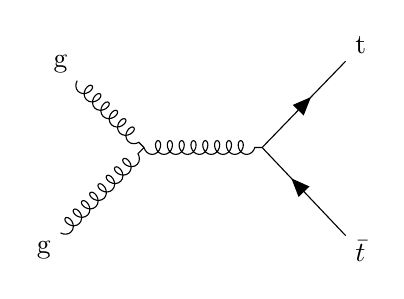
\begin{tikzpicture}
  \begin{feynman}   	
	\vertex (g1) {g};    
    \vertex [below right=of g1] (a);
    \vertex [right=of a] (b);
  	\vertex (g2) [below left=of a] {g};
	\vertex (t1) [above right=of b] {t};
	\vertex (t2) [below right=of b] {$\bar t$};  
 
    \diagram* {
      (g1) -- [gluon] (a),
      (g2) -- [gluon] (a),
      (a) -- [gluon] (b),
	  (b) -- [fermion] (t1),
	  (b) -- [anti fermion] (t2)      
    };
  \end{feynman}
\end{tikzpicture}
}
\end{minipage} \hfill
\begin{minipage}[b]{.34\textwidth}
\resizebox{\textwidth}{!}{
\begin{tikzpicture}
  \begin{feynman}   	
	\vertex (q1) {$\bar q$};    
    \vertex [below right=of g1] (a);
    \vertex [right=of a] (b);
  	\vertex (q2) [below left=of a] {q};
	\vertex (t1) [above right=of b] {t};
	\vertex (t2) [below right=of b] {$\bar t$};  
 
    \diagram* {
      (q1) -- [anti fermion] (a),
      (q2) -- [fermion] (a),
      (a) -- [gluon] (b),
	  (b) -- [fermion] (t1),
	  (b) -- [anti fermion] (t2)      
    };
  \end{feynman}
\end{tikzpicture}
}
\end{minipage} \hfill
\begin{minipage}[b]{.22\textwidth}
\resizebox{\textwidth}{!}{
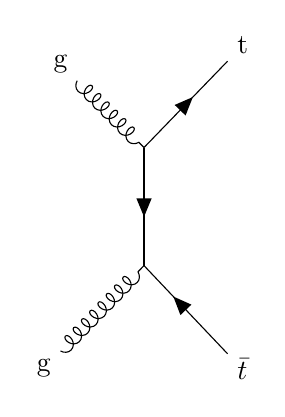
\begin{tikzpicture}
  \begin{feynman}   	
	\vertex (g1) {g};    
    \vertex (a) [below right=of g1];
    \vertex (b) [below=of a];
  	\vertex (g2) [below left=of b] {g};
	\vertex (t1) [above right=of a] {t};
	\vertex (t2) [below right=of b] {$\bar t$};  
 
    \diagram* {
      (g1) -- [gluon] (a),
      (g2) -- [gluon] (b),
      (a) -- [fermion] (b),
	  (a) -- [fermion] (t1),
	  (b) -- [anti fermion] (t2)      
    };
  \end{feynman}
\end{tikzpicture}
}
\end{minipage} \hfill
\caption{Main feynman diagrams for the production of the \ac{SM} $t \bar t$ process.}
\label{fig:ttbarProd}
\end{figure}

\subsubsection{Single top} \label{subsection:singleTop}

Different Feynman diagrams also account for this process in the s-channel (Figure~\ref{fig:singleTopSChann}), t-channel and tW production modes (Figure~\ref{fig:singleTopOtherChann}).

\begin{figure}[htbp]
\centering
\begin{minipage}[b]{.22\textwidth}
\resizebox{\textwidth}{!}{
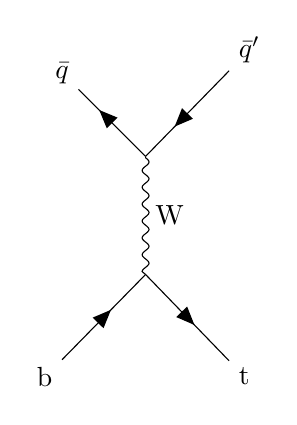
\begin{tikzpicture}
  \begin{feynman}   	
	\vertex (qi) {$\bar q$};    
    \vertex (a) [below right=of qi];
    \vertex (qf) [above right=of a] {$\bar q'$};    
  	\vertex (b) [below=of a];
	\vertex (bi) [below left=of b] {b};
	\vertex (tf) [below right=of b] {t};  
 
    \diagram* {
      (qi) -- [anti fermion] (a) -- [anti fermion] (qf),
      (a) -- [boson, edge label={W}] (b),
      (bi) -- [fermion] (b) -- [fermion] (tf)     
    };
  \end{feynman}
\end{tikzpicture}
}
\end{minipage} 
\begin{minipage}[b]{.28\textwidth}
\resizebox{\textwidth}{!}{
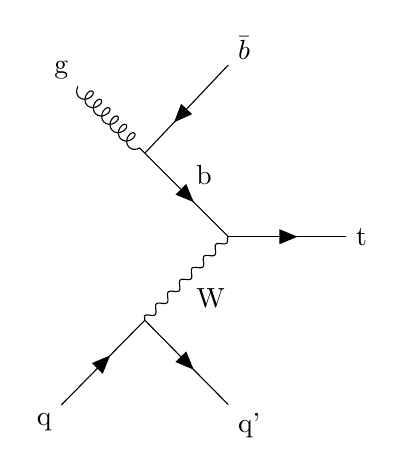
\begin{tikzpicture}
  \begin{feynman}   	
	\vertex (gi) {g};    
    \vertex (a) [below right=of gi];
    \vertex (bf) [above right=of a] {$\bar b$};
  	\vertex (b) [below right=of a];
  	\vertex (tf) [right=of b] {t};
	\vertex (c) [below left=of b];
	\vertex (qi) [below left=of c] {q};
	\vertex (qf) [below right=of c] {q'};  
 
    \diagram* {
      (gi) -- [gluon] (a) -- [anti fermion] (bf),
      (a) -- [fermion, edge label={b}] (b),
      (b) -- [fermion] (tf),
	  (b) -- [boson, edge label={W}] (c),
	  (qi) -- [fermion] (c) -- [fermion] (qf)      
    };
  \end{feynman}
\end{tikzpicture}
}
\end{minipage} 
\caption{Feynman diagrams for the s-channel production mode of a single top quark.}
\label{fig:singleTopSChann}
\end{figure}

\begin{figure}[htbp]
\centering
\begin{minipage}[b]{.34\textwidth}
\resizebox{\textwidth}{!}{
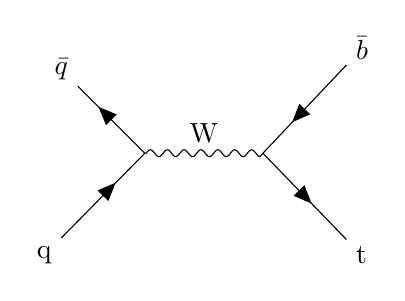
\begin{tikzpicture}
  \begin{feynman}   	
	\vertex (qi1) {$\bar q$};    
    \vertex (a) [below right=of qi1];
    \vertex (qi2) [below left=of a] {q};
  	\vertex (b) [right=of a];
  	\vertex (bf) [above right=of b] {$\bar b$};
	\vertex (tf) [below right=of b] {t}; 
 
    \diagram* {
      (qi1) -- [anti fermion] (a) -- [anti fermion] (qi2),
      (a) -- [boson, edge label={W}] (b),
      (b) -- [anti fermion] (bf),
	  (b) -- [fermion] (tf)    
    };
  \end{feynman}
\end{tikzpicture}
}
\end{minipage} 
\begin{minipage}[b]{.34\textwidth}
\resizebox{\textwidth}{!}{
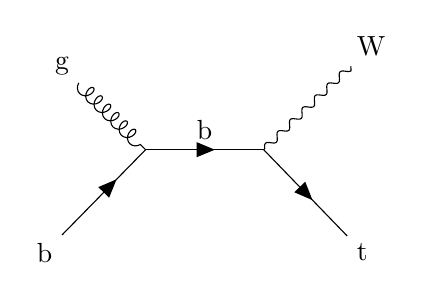
\begin{tikzpicture}
  \begin{feynman}   	
	\vertex (gi) {g};    
    \vertex (a) [below right=of gi];
    \vertex (bi) [below left=of a] {b};
  	\vertex (b) [right=of a];
	\vertex (Wf) [above right=of b] {W};
	\vertex (tf) [below right=of b] {t};  
 
    \diagram* {
      (gi) -- [gluon] (a) -- [anti fermion] (bi),
      (a) -- [fermion, edge label={b}] (b),
	  (b) -- [boson] (Wf),
	  (b) -- [fermion] (tf)      
    };
  \end{feynman}
\end{tikzpicture}
}
\end{minipage} 
\caption{Feynman diagrams for the t-channel (on the left) and tW (on the right) production modes of a single top quark.}
\label{fig:singleTopOtherChann}
\end{figure}

\subsubsection{Top decay} \label{subsection:topDecay}

As previously mentioned, the top is the heaviest particle of the \ac{SM} and is expected to decay inside of the beam pipe itself, usually into a bottom quark, giving us a b-jet, and a W boson; this boson can decay itself into different channels even though only its leptonic decay is consider in this particular case. The decay considered for the top/antitop produced is represented in Figure~\ref{fig:TopDecay}.

\begin{figure}[htbp]
\centering
\begin{minipage}[b]{.34\textwidth}
\resizebox{\textwidth}{!}{
\begin{tikzpicture}
  \begin{feynman}   	
	\vertex (ti) {t};    
    \vertex (a) [right=of ti];
    \vertex (W) [above right=of a];
  	\vertex (bf) [below right=of a] {b};
  	\vertex (b) [above right=of a];
	\vertex (lf) [above right=of b] {$l^+$};
	\vertex (nu) [below right=of b] {$\nu$};  
 
    \diagram* {
      (ti) -- [fermion] (a),
      (a) -- [boson, edge label={$W^+$}] (b),
      (a) -- [fermion] (bf),
	  (b) -- [fermion] (lf),
	  (b) -- [fermion] (nu)      
    };
  \end{feynman}
\end{tikzpicture}
}
\end{minipage} 
\begin{minipage}[b]{.34\textwidth}
\resizebox{\textwidth}{!}{
\begin{tikzpicture}
  \begin{feynman}   	
	\vertex (ti) {$\bar t$};    
    \vertex (a) [right=of ti];
    \vertex (W) [above right=of a];
  	\vertex (bf) [below right=of a] {$\bar b$};
  	\vertex (b) [above right=of a];
	\vertex (lf) [above right=of b] {$l^-$};
	\vertex (nu) [below right=of b] {$\bar \nu$};  
 
    \diagram* {
      (ti) -- [fermion] (a),
      (a) -- [boson, edge label={$W^-$}] (b),
      (a) -- [fermion] (bf),
	  (b) -- [fermion] (lf),
	  (b) -- [fermion] (nu)      
    };
  \end{feynman}
\end{tikzpicture}
}
\end{minipage} 
\caption{Feynman diagrams for the leptonic decay of the top (on the left) and antitop (on the right) quarks.}
\label{fig:TopDecay}
\end{figure}

\subsection{Drell-Yan estimation} \label{subsection:DY}

As previously mentioned, most of the \ac{DY}, produced through the Feynman diagram represented in Figure~\ref{fig:DY}, is not expected to survive the selection applied to the analysis. However, because of the huge cross section of this process, two to three orders of magnitude larger than the production of a top, a thorough description of such process is still extremely important.

\begin{figure}[htbp]
\centering
\begin{minipage}[b]{.34\textwidth}
\resizebox{\textwidth}{!}{
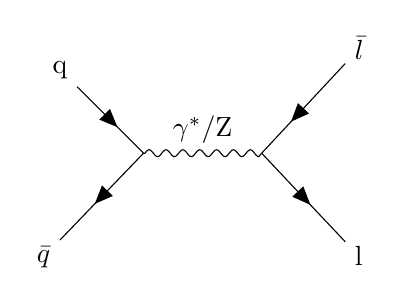
\begin{tikzpicture}
  \begin{feynman}   	
	\vertex (qi1) {q};
	\vertex (a) [below right=of qi1];    
    \vertex (qi2) [below left=of a] {$\bar q$};
    \vertex (b) [right=of a]; 
    \vertex (lf1) [above right=of b] {$\bar l$};
    \vertex (lf2) [below right=of b] {l};
 
    \diagram* {
      (qi1) -- [fermion] (a) -- [fermion] (qi2),
      (a) -- [boson, edge label={$\gamma^*$/Z}] (b),
	  (b) -- [anti fermion] (lf1),
	  (b) -- [fermion] (lf2)      
    };
  \end{feynman}
\end{tikzpicture}
}
\end{minipage} 
\caption{Feynman diagram for the \ac{DY} process involving a virtual $\gamma^*$ or Z boson.}
\label{fig:DY}
\end{figure}

This background is also estimated from \ac{MC} as well and is being checked in a specific control region as well, as described in Section~\ref{section:CR}.

\subsection{$t \bar t + V$} \label{subsection:ttV}

This background is coming from a usual $t \bar t$ production along with an \acp{ISR} or \ac{FSR} production of a W or Z boson, as shown in Figure~\ref{fig:ttV}. The contribution of this background is also taken directly from \ac{MC}.

\begin{figure}[htbp]
\centering
\begin{minipage}[b]{.31\textwidth}
\resizebox{\textwidth}{!}{
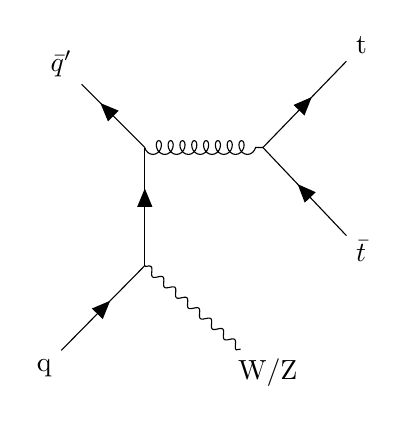
\begin{tikzpicture}
  \begin{feynman}   	
	\vertex (qi1) {$\bar q'$};    
    \vertex (a) [below right=of qi1];
    \vertex (gf) [right=of a];
    \vertex (b) [below=of a];
  	\vertex (qi2) [below left=of b] {q};
  	\vertex (Wf) [below right=of b] {W/Z};
  	\vertex (c) [right of=a];
  	\vertex (tf1) [above right=of c] {t};
  	\vertex (tf2) [below right=of c] {$\bar t$};
 
    \diagram* {
      (qi1) -- [anti fermion] (a) -- [gluon] (c) -- [fermion] (tf1),
      (tf2) -- [fermion] (c),
      (a) -- [anti fermion] (b),
      (qi2) -- [fermion] (b) -- [boson] (Wf)    
    };
  \end{feynman}
\end{tikzpicture}
}
\end{minipage} 
\begin{minipage}[b]{.34\textwidth}
\resizebox{\textwidth}{!}{
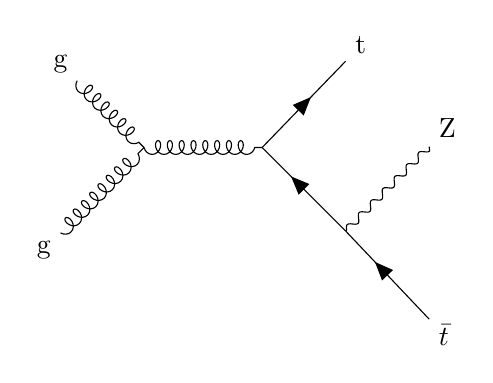
\begin{tikzpicture}
  \begin{feynman}   	
	\vertex (gi1) {g};    
    \vertex (a) [below right=of gi1];
    \vertex (gi2) [below left=of a] {g}; 
    \vertex (b) [right=of a];
    \vertex (tf1) [above right=of b] {t};
  	\vertex (c) [below right=of b];
  	\vertex (Zf) [above right=of c] {Z};
  	\vertex (tf2) [below right=of c] {$\bar t$};
 
    \diagram* {
      (gi1) -- [gluon] (a) -- [gluon] (b),
      (gi2) -- [gluon] (a),
      (b) -- [fermion] (tf1),
      (b) -- [anti fermion] (c) -- [anti fermion] (tf2),
      (c) -- [boson] (Zf)
    };
  \end{feynman}
\end{tikzpicture}
}
\end{minipage} 
\begin{minipage}[b]{.29\textwidth}
\resizebox{\textwidth}{!}{
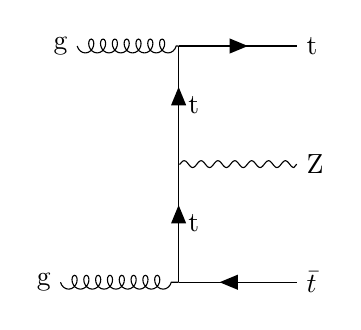
\begin{tikzpicture}
  \begin{feynman}   	
	\vertex (gi1) {g};    
    \vertex (a) [right=of gi1];
    \vertex (b) [below=of a];
    \vertex (c) [below=of b];
    \vertex (gi2) [left=of c] {g};
    \vertex (Zf) [right=of b] {Z};
    \vertex (tf1) [right=of a] {t};
  	\vertex (tf2) [right=of c] {$\bar t$};
 
    \diagram* {
      (gi1) -- [gluon] (a) -- [fermion] (tf1),
      (gi2) -- [gluon] (c) -- [anti fermion] (tf2),
      (a) -- [anti fermion, edge label={t}] (b) -- [anti fermion, edge label={t}] (c),  
      (b) -- [boson] (Zf) 
    };
  \end{feynman}
\end{tikzpicture}
}
\end{minipage} 
\caption{Possible Feynman diagrams for the \ac{ISR} $t \bar t$ with a W/Z boson (on the left) and for the production of an \ac{FSR} ttZ (on the center and right).}
\label{fig:ttV}
\end{figure}

The resulting cross section of such process is a bit lower than the production of the \ac{SM} $t \bar t$ on its own but the kinematics of this background can be extremely close to our signal, since the W or Z boson produced can give a \ac{SM} neutrino, leading to some actual \ac{MET}.

\subsection{Non prompt contamination} \label{subsection:Fakes}

Even though not extremely important in the sense that its kinematics allow us to remove most of its contributions in the signal regions, this background is interesting in the sense that is can be estimated using a data-driven method instead of being taken directly from \ac{MC}.

A few definitions are first of all needed to explain the method used to compute the importance of this background in the different regions of the analysis:
\begin{itemize}
\item First of all, a \textbf{prompt lepton} is defined as a real lepton, in the sense that the lepton is originating from the \ac{PV} of a $pp$ collision.
\item The \textbf{\ac{PR}} is defined as the number of prompt leptons passing the tight selection criteria of the analysis over the number of leptons passing the loose selection criteria. 
\item On the other hand, by \textbf{fake} or \textbf{non-prompt lepton}, we usually refer to truly \textbf{fake leptons}, such as jets misidentified by the detector as leptons, as shown in Figure~\ref{fig:FakesW}, and real leptons coming from eventual heavy flavor decays.
\item The \textbf{\ac{FR}} is then defined similarly to the prompt rate but considering this time fake leptons only for the tight-to-loose ratio. This ratio therefore corresponds to the probability for a fake lepton to be considered as a real lepton in the analysis.
\end{itemize}

\begin{figure}[htbp]
\centering
\begin{minipage}[b]{.19\textwidth}
\resizebox{\textwidth}{!}{
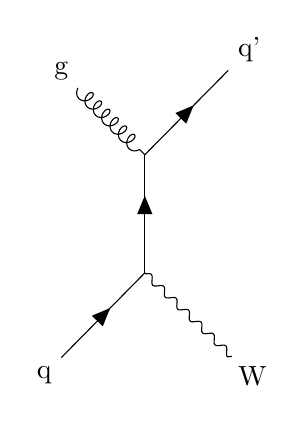
\begin{tikzpicture}
  \begin{feynman}   	
	\vertex (gi) {g};    
    \vertex (a) [below right=of gi];
    \vertex (qf) [above right=of a] {q'};
    \vertex (b) [below=of a];
  	\vertex (qi) [below left=of b] {q};
  	\vertex (Wf) [below right=of b] {W};
 
    \diagram* {
      (gi) -- [gluon] (a) -- [fermion] (qf),
      (a) -- [anti fermion] (b),
      (qi) -- [fermion] (b) -- [boson] (Wf)    
    };
  \end{feynman}
\end{tikzpicture}
}
\end{minipage} 
\begin{minipage}[b]{.22\textwidth}
\resizebox{\textwidth}{!}{
\begin{tikzpicture}
  \begin{feynman}   	
	\vertex (qi1) {$\bar q'$};    
    \vertex (a) [below right=of qi1];
    \vertex (gf) [above right=of a] {g};
    \vertex (b) [below=of a];
  	\vertex (qi2) [below left=of b] {q};
  	\vertex (Wf) [below right=of b] {W/Z};
 
    \diagram* {
      (qi1) -- [anti fermion] (a) -- [gluon] (qf),
      (a) -- [anti fermion] (b),
      (qi2) -- [fermion] (b) -- [boson] (Wf)    
    };
  \end{feynman}
\end{tikzpicture}
}
\end{minipage} 
\begin{minipage}[b]{.31\textwidth}
\resizebox{\textwidth}{!}{
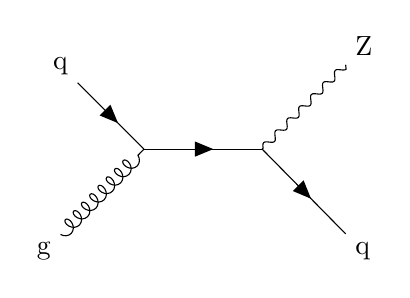
\begin{tikzpicture}
  \begin{feynman}   	
	\vertex (qi) {q};    
    \vertex (a) [below right=of qi];
    \vertex (gi) [below left=of a] {g};
    \vertex (b) [right=of a];
  	\vertex (Z) [above right=of b] {Z};
  	\vertex (q) [below right=of b] {q};
 
    \diagram* {
      (qi) -- [fermion] (a),
      (gi) -- [gluon] (a),
      (a) -- [fermion] (b),
      (b) -- [boson] (Z),
      (b) -- [fermion] (q)    
    };
  \end{feynman}
\end{tikzpicture}
}
\end{minipage} 
\caption{Possible Feynman diagrams for the production of a W/Z boson with a jet.}
\label{fig:FakesW}
\end{figure}

This background is particularly important at low $p_T$, where the misidentification rate is higher, and is not expected to be modeled correctly by \ac{MC} because of its complexity: a general \textbf{tight-to-loose data-driven method} is then used to compute its kinematics and final contribution in the different regions of the analysis. 

In general, this method contains three main steps: the computation of the \ac{FR} and \ac{PR}, the extension of these rates in a region kinematically close to the \ac{SR} of the analysis and the definition of a same sign control region enriched in fakes in order to perform a closure test of the yields and kinematics of this background.% All these steps will now be detailed.

\subsubsection*{\acf{FR} computation}

Because of its definition, the \ac{FR} is computed in a prompt lepton-free region, typically in a l1loose \ac{QCD} enriched region, defined with the following cuts:
\begin{multicols}{2}
\begin{itemize}
\item Exactly 1 lepton
\item $p_{T} > 13 \text{ } (10)$ GeV for $e \text{ }(\mu)$ 
\item $|\eta| < 2.5 \text{ } (2.4)$ for $e \text{ }(\mu)$ 
\item mtw1 $< 20$ GeV
\item PuppiMET $< 20$ GeV
\item PassJets
\end{itemize}
\end{multicols}

All the previous cuts have been designed to define a l1loose \ac{QCD} region as pure as possible by removing most of the W+jets and Z+jets contribution. The PassJets cut is a boolean obtained by looping over all the jets of the event trying to find a jet having an $E_T$ higher than a given threshold in order to control the average $p_T$ of the jet that fakes the lepton (actually, different \ac{FR} have been computed for different $E_T$ thresholds, from 10 to 50 GeV). 

Using this method, the jet that fakes a lepton is actually the one recoiling against ($\Delta R > 1.0$) the jet used for the systematics, as shown in Figure~\ref{fig:FakesJet}.

\begin{figure}[htbp]
\begin{center}
\includegraphics[width=8cm, height=4cm]{figs/FakesJet.png}
\caption{Schematic representation of the two jets used for the systematics and for the jet faking a lepton in the tight-to-loose data-driven method.}
\label{fig:FakesJet}
\end{center}
\end{figure}

Events passing the following pre-scaled triggers are then selected in this region:

\begin{subequations}
\begin{equation}
\text{Muon triggers = }
\begin{dcases}
\text{HLT\_Mu8\_TrkIsoVVL (if }p_T < 20 \text{ GeV}) \\
\text{HLT\_Mu17\_TrkIsoVVL (if }p_T \geq 20 \text{ GeV}) 
\end{dcases}
\end{equation}
\vspace{-20pt}
\begin{equation}
\text{Electron triggers = }
\begin{dcases}
\text{HLT\_Ele8\_CaloIdL\_TrackIdL\_IsoVL\_PFJet30 (if }p_T < 25 \text{ GeV}) \\
\text{HLT\_Ele23\_CaloIdL\_TrackIdL\_IsoVL\_PFJet30 (if }p_T \geq 25 \text{ GeV}) 
\end{dcases}
\end{equation}
\end{subequations}

The remaining of the \ac{EWK} processes (W+jets, Z+jets) able to pass the previous cuts of the QCD region, are then simply subtracted: this is the so-called \textbf{\ac{EWK} subtraction}.

Since both the \ac{FR} and \ac{PR} heavily depend on the kinematics of the event and on the \acf{WP} chosen for the leptons of the analysis, they are computed separately depending on the flavor of the lepton and 2D histograms (accounting for the $p_T$ and $\eta$ of the lepton) need to be created at this stage to calculate this factor, for a given input jet $E_T$ threshold; 1D histograms corresponding to the projections of these 2D histograms along both their axes are also defined at this point, as shown in Figure~\ref{fig:FR}.

\begin{figure}[htbp]
\centering
\subfigure[2016 electron and muon fake rates]
 {
\begin{minipage}[b]{.48\textwidth}
\includegraphics[width=7cm, height=7cm]{figs/Ele_FR_pt_combined_2016.png}
\end{minipage}\hfill
\begin{minipage}[b]{.48\textwidth}
\includegraphics[width=7cm, height=7cm]{figs/Muon_FR_pt_combined_2016.png}
\end{minipage} \hfill
}
\subfigure[2017 electron and muon fake rates]
 {
\begin{minipage}[b]{.48\textwidth}
\includegraphics[width=7cm, height=7cm]{figs/Ele_FR_pt_combined_2017.png}
\end{minipage}\hfill
\begin{minipage}[b]{.48\textwidth}
\includegraphics[width=7cm, height=7cm]{figs/Muon_FR_pt_combined_2017.png}
\end{minipage} \hfill
}
\subfigure[2018 electron and muon fake rates]
 {
\begin{minipage}[b]{.48\textwidth}
\includegraphics[width=7cm, height=7cm]{figs/Ele_FR_pt_combined_2018.png}
\end{minipage}\hfill
\begin{minipage}[b]{.48\textwidth}
\includegraphics[width=7cm, height=7cm]{figs/Muon_FR_pt_combined_2018.png}
\end{minipage} \hfill
}
\caption{Electron (on the left) and muon (on the right) \ac{FR} obtained in a QCD enriched region for different jet $E_T$ thresholds for 2016, 2017 and 2018 with respect to the $p_T$ of the lepton.}
\label{fig:FR}
\end{figure}

\subsubsection*{\acf{PR} computation}

The \ac{PR}, taking into account the real lepton contamination in the region defined, is also important to calculate, even though the objects \ac{WP} are usually chosen is such a way that this ratio is quite close to 1 and can therefore typically be ignored.

In our case, this rate has been calculated as well using a general tag and probe method in a Z+jets enriched sample. The main objective is to reconstruct $Z \rightarrow ll$ events in this region and to select all the events for which the first lepton can be characterized as tight. Then, we search for the second lepton coming from the decay of Z within all the leptons detected by calculating the reconstructed mass of all the possible leptons combinations and selecting the one which is closer to the expected mass of the Z boson. We can then simply count how many times this second lepton, expected to be tight, has actually been measured as a tight lepton to estimate this \ac{PR}.

The results obtained in this case have been represented in Figure~\ref{fig:PR}.

\begin{figure}[htbp]
\centering
\subfigure[2016 electron and muon prompt rates]
 {
\begin{minipage}[b]{.48\textwidth}
\includegraphics[width=7cm, height=7cm]{figs/Ele_PR_pt_2016.png}
\end{minipage}\hfill
\begin{minipage}[b]{.48\textwidth}
\includegraphics[width=7cm, height=7cm]{figs/Muon_PR_pt_2016.png}
\end{minipage} \hfill
}
\subfigure[2017 electron and muon prompt rates]
 {
\begin{minipage}[b]{.48\textwidth}
\includegraphics[width=7cm, height=7cm]{figs/Ele_PR_pt_2017.png}
\end{minipage}\hfill
\begin{minipage}[b]{.48\textwidth}
\includegraphics[width=7cm, height=7cm]{figs/Muon_PR_pt_2017.png}
\end{minipage} \hfill
}
\subfigure[2018 electron and muon prompt rates]
 {
\begin{minipage}[b]{.48\textwidth}
\includegraphics[width=7cm, height=7cm]{figs/Ele_PR_pt_2018.png}
\end{minipage}\hfill
\begin{minipage}[b]{.48\textwidth}
\includegraphics[width=7cm, height=7cm]{figs/Muon_PR_pt_2018.png}
\end{minipage} \hfill
}
\caption{Electron (on the left) and muon (on the right) \ac{PR} obtained in a Z+jets enriched region by a tag and probe method for 2016, 2017 and 2018 with respect to the $p_T$ of the lepton.}
\label{fig:PR}
\end{figure}

\subsubsection*{Fake weight calculation}

Once the fake and prompt rates computed in their specific region, it is still necessary to apply them to a fake-lepton region kinematically close to the \acp{SR} of the analysis (usually, a l2loose region). For this, a simple set of equations can be used. We start by defining the following quantities:

\begin{itemize}
\item $N_{pp}$, the number of events where both leptons are prompt
\item $N_{fp}$, the number of events where one lepton is prompt and the other is fake
\item $N_{ff}$, the number of events where both leptons are fake
\item $N_{tx}$ ($x = 0,1,2$), the number of events with 0, 1 or 2 leptons passing the right cuts, the \textbf{only quantity directly measurable} by the detector
\end{itemize}

It is then possible to see in Equation~\ref{eq:FR1} that, if $p$ is the \ac{PR} and $f$ the \ac{FR} previously calculated, we can find an expression relating all these quantities.
\begin{equation}
\label{eq:FR1}
\begin{dcases}
&N_l = N_{pp} + N_{fp} + N_{ff} = N_{t2} + N_{t1} + N_{t0} \\
& N_{t0} = (1-p)^2N_{pp} + (1-p)(1-f)N_{fp}+(1-f)^2N_{ff} \\
& N_{t1} = 2p(1-p)N_{pp} + \big(f(1-p)+p(1-f)\big)N_{fp}+2f(1-f)^2N_{ff} \\
& N_{t2} = p^2N_{pp} + pfN_{fp}+f^2N_{ff}
\end{dcases}
\end{equation}

These equations can be inverted in order to represent the unknowns with respect to the known variables, as shown in Equation~\ref{eq:FR2}, giving us a way to apply the weights previously calculated to this particular l2loose region.

\begin{equation}
\label{eq:FR2}
\begin{pmatrix}
N_{pp} \\ N_{fp} \\ N_{ff}
\end{pmatrix} = \frac{f-p}{-(p-f)^3} \cdot 
\begin{pmatrix}
f^2 & -f(1-f) & (1-f)^2 \\ -2fp & p(1-f)+f(1-p) & -2(1-p)(1-f) \\ p^2 & -p(1-p) & (1-p)^2
\end{pmatrix} \cdot 
\begin{pmatrix}
N_{t0} \\ N_{t1} \\ N_{t2}
\end{pmatrix}
\end{equation}

\subsubsection*{Same sign control region}

Now that we have a way to estimate the kinematics and yields of the non-prompt background in a different region, a same sign \ac{CR} enriched in fakes is usually defined in order to check this background. This will be done and detailed in Section~\ref{section:SSCR} of this work.

%\subsubsection*{Limitations}
%
%This method is working quite well and allows us to avoid relying on the \ac{MC} for such complex processes, but it does come with some limitations, among which:
%
%\begin{itemize}
%\item 
%\end{itemize}

\subsection{Smaller backgrounds} \label{subsection:SmallerBkg}

Even though quite negligible and reducible, some additional backgrounds still need to be considered, such as the \ac{SM} $t \bar t$ decaying semi-leptonically, the dibosons (WW, WZ and ZZ) and tribosons (WWW, WWZ, WZZ, ZZZ) productions, as shown in Figure~\ref{fig:DiBosons}. Backgrounds such as the W$\gamma$ and Higgs related productions are also considered at this stage. All these smaller backgrounds are taken directly from \ac{MC} and account in total for less than 1\% of the total backgrounds in the different signal regions. 

\begin{figure}[htbp]
\centering
\begin{minipage}[b]{.31\textwidth}
\resizebox{\textwidth}{!}{
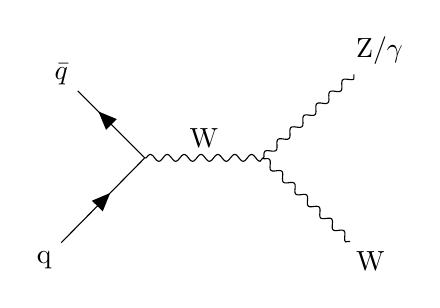
\begin{tikzpicture}
  \begin{feynman}   	
	\vertex (qi1) {$\bar q$};    
    \vertex (a) [below right=of qi1];
    \vertex (qi2) [below left=of a] {q};
    \vertex (b) [right=of a];
    \vertex (Zf) [above right=of b] {Z/$\gamma$};
    \vertex (Wf) [below right=of b] {W};
 
    \diagram* {
      (qi1) -- [anti fermion] (a),
      (qi2) -- [fermion] (a) -- [boson, edge label={W}] (b),
      (b) -- [boson] (Zf),
      (b) -- [boson] (Wf)  
    };
  \end{feynman}
\end{tikzpicture}
}
\end{minipage} 
\begin{minipage}[b]{.34\textwidth}
\resizebox{\textwidth}{!}{
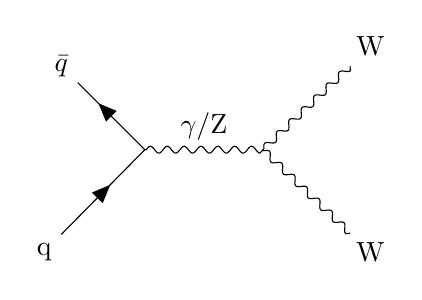
\begin{tikzpicture}
  \begin{feynman}   	
	\vertex (qi1) {$\bar q$};    
    \vertex (a) [below right=of qi1];
    \vertex (qi2) [below left=of a] {q};
    \vertex (b) [right=of a];
    \vertex (Zf) [above right=of b] {W};
    \vertex (Wf) [below right=of b] {W};
 
    \diagram* {
      (qi1) -- [anti fermion] (a),
      (qi2) -- [fermion] (a) -- [boson, edge label={$\gamma$/Z}] (b),
      (b) -- [boson] (Zf),
      (b) -- [boson] (Wf)  
    };
  \end{feynman}
\end{tikzpicture}
}
\end{minipage} 
\begin{minipage}[b]{.22\textwidth}
\resizebox{\textwidth}{!}{
\begin{tikzpicture}
  \begin{feynman}   	
	\vertex (qi1) {$\bar q$};
    \vertex (a) [below right=of qi1];
    \vertex (Zf1) [above right=of a] {Z};
    \vertex (b) [below=of a];
    \vertex (qi2) [below left=of b] {q};
    \vertex (Zf2) [below right=of b] {Z};
 
    \diagram* {
      (qi1) -- [anti fermion] (a) -- [boson] (Zf1),
      (qi2) -- [fermion] (b) -- [boson] (Zf2),
      (a) -- [anti fermion] (b)
    };
  \end{feynman}
\end{tikzpicture}
}
\end{minipage} 
\caption{Possible Feynman diagrams for smaller backgrounds of this analysis: WW (on the left), W$\gamma$ and WZ (on the center) and ZZ (on the right).}
\label{fig:DiBosons}
\end{figure}

\subsection{Weights and corrections applied} \label{subsection:Weights}

Several different weights and \ac{SF} usually need to be applied to the different \ac{MC} processes in order to account for several effects observed in data but not accounted for during the generation of the \ac{MC} simulation, such as the efficiency of the selection of the different objects, which will be discussed in Chapter~\ref{chapter:Selection}, usually directly provided by the different \acfp{POG} for their own default objects definitions.  The \ac{MC} samples are additionally typically reweighted to match the distribution of true interactions observed in data due to multiple collisions collisions happening in the same bunch-crossings (the \ac{PU}, as defined in Section~\ref{subsection:PU}). To illustrate the effect of these corrections, two particular weights that are applied to the \ac{MC} samples will now be detailed.

\subsubsection{Prefiring corrections}

In 2016 and 2017 an issue, known as the \textbf{prefiring}, causing highly energetic readout from jets, photons and electrons in the \ac{ECAL} endcap to be assigned by the \ac{L1} trigger to the previous bunch crossing was discovered. To make up for this difference, a weight ($1-x$) is usually applied to all \ac{MC} events, where $x$ is the probability of an event to be prefired \cite{Prefire}. The effect this correction has on the data/\ac{MC} agreement in a 2017 top enriched control region is shown in Figure~\ref{fig:Prefiring}.

\begin{figure}[htbp]
\begin{center}
\includegraphics[width=14cm, height=6cm]{figs/Prefiring.png}
\caption{Data/\ac{MC} agreement without (on the left) and with (on the right) prefiring corrections in a general 2018 top control region.}
\label{fig:Prefiring}
\end{center}
\end{figure}

\subsubsection{Top $p_T$ reweighting}

Previous studies of the $t \bar t$ generator typically considered in the physics analysis predict a harder top quark $p_T$ spectrum than the one observed in data \cite{topPt}. This known mismodeling of the top quark is corrected using a general reweighting recipe \cite{TopPtRecipe}, and its effect on the $p_T$ spectrum can be observed in Figure~\ref{fig:Toppt}.

\begin{figure}[htbp]
\begin{center}
\begin{minipage}[b]{.48\textwidth}
\includegraphics[width=7cm, height=6cm]{figs/cratio_topCR_df_2j_pt1_without.png}
\end{minipage} \hfill
\begin{minipage}[b]{.48\textwidth}
\includegraphics[width=7cm, height=6cm]{figs/cratio_topCR_df_2j_pt1_with.png}
\end{minipage} \hfill
\caption{Data/\ac{MC} agreement without (on the left) and with (on the right) top $p_T$ reweighting corrections in a general 2017 top control region.}
\label{fig:Toppt}
\end{center}
\end{figure}






























\chapter{Event selection} \label{chapter:Selection}

This Chapter will be dedicated to the analysis itself, by defining first of all the different objects actually used in this case, along with the actual selection that has been applied to enhance the quality of such objects in this particular search in Section~\ref{section:Selection}. Then, the different \acfp{SR} defined in which a high purity of signal is expected are defined in Section~\ref{section:SR} while all the different \acfp{CR} defined in order to check the behavior of the \ac{MC} simulation performed for the major backgrounds on this analysis, such as the single top or \ac{SM} $t \bar t$ production, will be introduced in Section~\ref{section:CR}. 

\section{Objects selection} \label{section:Selection}

We already described what to expect from a typical $t/\bar t$ or $t \bar t$+DM signal: the typical signature of such signals is made out of a certain number of b tagged jets along with two leptons (electrons and/or muons) and some \ac{MET} coming from the two \ac{DM} particles created along the way. It is therefore extremely important to describe the \ac{WP} chosen and the selection applied in order to select the objects of the analysis, such as the leptons and the jets used, in such a way to optimize the lepton reconstruction efficiency while reducing as much as possible the possible misidentification rates of such objects.

First of all, the different triggers used to collect the data will be detailed in Section~\ref{section:Triggers}. Then, the leptons used in this analysis will be introduced in Sections~\ref{section:EleSel} (for electrons) and~\ref{section:MuSel} (for muons). Finally, given the nature of the \ac{DM} signal searched for, a complete description of the jets selected in the analysis will be necessary and performed in Section~\ref{section:JetSel}.

\subsection{Triggers selection} \label{section:Triggers}

The triggers, described in Section~\ref{subsection:Trigger}, and particularly the trigger paths chosen are an important part of each analysis since they will describe the kind of data that can be collected and therefore analyzed. The triggers used in this analysis for the years 2016, 2017 and 2018 can be found in Tables~\ref{table:Trigg2016},~\ref{table:Trigg2017} and~\ref{table:Trigg2016} respectively.

\begin{table}
\begin{center}
%\resizebox{\textwidth}{!}{
\begin{tabular}{ l|l|l } 
 \hline
 Dataset & Run range & \textbf{\ac{HLT} trigger path} \\
 \hline
 \multirow{1}{*}{SingleMu} & \multirow{1}{*}{[273158,284044]}  & HLT\_IsoMu24\_v* \\
& & HLT\_IsoTkMu24\_v* \\
\hline
\multirow{1}{*}{SingleEle} & \multirow{1}{*}{[273158,284044]} & HLT\_Ele27\_WPTight\_Gsf\_v* \\
& & HLT\_Ele25\_eta2p1\_WPTight\_Gsf\_v* \\
\hline
DoubleEG & [273158,284044] & HLT\_Ele23\_Ele12\_CaloIdL\_TrackIdL\_IsoVL\_DZ\_v* \\
\hline
\multirow{1}{*}{DoubleMu} & \multirow{1}{*}{[273158,281612]} & HLT\_Mu17\_TrkIsoVVL\_Mu8\_TrkIsoVVL\_v* \\
& & HLT\_Mu17\_TrkIsoVVL\_TkMu8\_TrkIsoVVL\_v* \\
& \multirow{1}{*}{[281613,284044] }& HLT\_Mu17\_TrkIsoVVL\_Mu8\_TrkIsoVVL\_DZ\_v* \\
& & HLT\_Mu17\_TrkIsoVVL\_TkMu8\_TrkIsoVVL\_DZ\_v* \\
\hline
\multirow{1}{*}{MuonEG} & \multirow{1}{*}{[273158,278272]} & HLT\_Mu8\_TrkIsoVVL\_Ele23\_CaloIdL\_TrackIdL\_IsoVL \\
& & HLT\_Mu23\_TrkIsoVVL\_Ele12\_CaloIdL\_TrackIdL\_IsoVL \\
 & \multirow{1}{*}{[278273,284044]} & HLT\_Mu8\_TrkIsoVVL\_Ele23\_CaloIdL\_TrackIdL\_IsoVL\_DZ\_v* \\
& & HLT\_Mu23\_TrkIsoVVL\_Ele12\_CaloIdL\_TrackIdL\_IsoVL\_DZ\_v* \\
\hline
\end{tabular}
%}
\caption{2016 trigger paths considered for this analysis.}
\label{table:Trigg2016}
\end{center}
\end{table}	

\begin{table}
\begin{center}
%\resizebox{\textwidth}{!}{
\begin{tabular}{ l|l|l } 
 \hline
 Dataset &Run range & \textbf{\ac{HLT} trigger path} \\
\hline
 SingleMu & [297046,306462]  & HLT\_IsoMu27\_v* \\
\hline
EGamma & [297046,306462] & HLT\_Ele35\_WPTight\_Gsf\_v* \\
& & HLT\_Ele23\_Ele12\_CaloIdL\_TrackIdL\_IsoVL\_v* \\
\hline
DoubleMu & [297046,299329] & HLT\_Mu17\_TrkIsoVVL\_Mu8\_TrkIsoVVL\_DZ\_v* \\
& [299368,306462] & HLT\_Mu17\_TrkIsoVVL\_Mu8\_TrkIsoVVL\_DZ\_Mass8\_v* \\
\hline
\multirow{1}{*}{MuonEG} & [297046,306462] & HLT\_Mu12\_TrkIsoVVL\_Ele23\_CaloIdL\_TrackIdL\_IsoVL\_DZ\_v* \\
& [297046,299329] & HLT\_Mu23\_TrkIsoVVL\_Ele12\_CaloIdL\_TrackIdL\_IsoVL\_DZ\_v* \\
& [299368,306462]  & HLT\_Mu23\_TrkIsoVVL\_Ele12\_CaloIdL\_TrackIdL\_IsoVL\_v* \\
\hline
\end{tabular}
%}
\caption{2017 trigger paths considered for this analysis.}
\label{table:Trigg2017}
\end{center}
\end{table}	

\begin{table}
\begin{center}
%\resizebox{\textwidth}{!}{
\begin{tabular}{ l|l|l } 
 \hline
 Dataset & Run range & \textbf{\ac{HLT} trigger path} \\
\hline
 SingleMu & [315252,325172] & HLT\_IsoMu24\_v* \\
 & & HLT\_Mu5\_v* \\
 & [314859,325175] & HLT\_IsoMu27\_v* \\
\hline
EGamma & [315252,325172] & HLT\_Ele32\_WPTight\_Gsf\_v* \\
& & HLT\_Ele35\_WPTight\_Gsf\_v* \\
& & HLT\_Ele23\_Ele12\_CaloIdL\_TrackIdL\_IsoVL\_v* \\
\hline
DoubleMu & [315252,325172] & HLT\_Mu17\_TrkIsoVVL\_Mu8\_TrkIsoVVL\_DZ\_Mass3p8\_v* \\
 &  & HLT\_Mu17\_TrkIsoVVL\_Mu8\_TrkIsoVVL\_DZ\_Mass8\_v* \\
\hline
\multirow{1}{*}{MuonEG} & [315252,325172] & HLT\_Mu23\_TrkIsoVVL\_Ele12\_CaloIdL\_TrackIdL\_IsoVL\_v* \\
& & HLT\_Mu12\_TrkIsoVVL\_Ele23\_CaloIdL\_TrackIdL\_IsoVL\_DZ\_v* \\
\hline
\end{tabular}
%}
\caption{2018 trigger paths considered for this analysis.}
\label{table:Trigg2018}
\end{center}
\end{table}	

Our analysis relying on the dilepton final state, the single lepton trigger are only considered in order to recover some of the efficiency lost in some cases when one lepton passes the tight identification criteria while the second one does not, and does therefore not trigger the event. The logical \textit{or} of all the trigger paths are usually considered. Eventual events passing several triggers is taken into account as well to make sure to avoid any double counting due to this effect.

These triggers have been studied in order to make sure that they are efficient enough in the $p_T$ region of the leptons of the analysis to avoid any undesired effect due to the turn-on of any trigger. These trigger efficiencies, calculated using a general tag and probe method and found for example for different runs of the 2017 data taking period in Figure~\ref{fig:TriggEffEle} for a DoubleEG trigger, are then used to reweight the simulated samples.

\begin{figure}[htbp]
\centering
\begin{minipage}[b]{.47\textwidth}
\includegraphics[width=6cm, height=5.5cm]{figs/TriggEffEle.png}
\end{minipage}\hfill
\begin{minipage}[b]{.47\textwidth}
\includegraphics[width=6cm, height=5.5cm]{figs/TriggEffEta.png}
\end{minipage} \hfill
\caption{DougleEG trigger efficiencies with respect to the $p_T$ (on the left) and $\eta$ (on the right), computed using a tag and probe method, for the 2017 data taking period.}
\label{fig:TriggEffEle}
\end{figure}

\subsection{Electrons selection} \label{section:EleSel}

Several strategies are used in \ac{CMS} in order to be able to identify prompts electrons and isolate this signal over background sources coming mainly from photon conversions, misidentification of jets or electrons coming from the semileptonic decay of the bottom and charm quarks. Several variables, which can be divided in the several following categories, allow to introduce some discrimination between these prompt and fake electrons:

\begin{itemize}
\item The \textbf{calorimetric observables} use the transverse shape of electromagnetic showers in the \ac{ECAL}, the fact that these electromagnetic showers should be narrower than hadronic showers and the fraction of energy deposited in the \ac{HCAL} and in the preshower/endcaps of the \ac{ECAL} itself for the discrimination. Many different variables belong to this category, such as:
\begin{itemize}
\item \textbf{hOverE} $\left ( \frac{H}{E} \right )$, where $H$ corresponds to the energy deposited in the \ac{HCAL} and $E$ the total energy deposited in the \ac{ECAL}.
\item \textbf{ooEmooP} $\left ( \frac{1}{E_{\text{SC}}} - \frac{1}{p} \right )$, where $E_{\text{SC}}$ is the \acf{SC} energy and $p$ the momentum of the track at the point of closest approach to the \ac{PV}.
\item \textbf{dEtaInSee} $\Delta \eta$ (\textbf{dPhiInSee} $\Delta \phi$), the $\eta$  ($\phi$) difference between the \ac{SC} and the inner track extrapolated from the interaction vertex.
%\item The \textbf{\ac{SC} $\eta$ ($\phi$) width}
\item \textbf{sigmaIetaIeta} ($\sigma_{\eta \eta}$), the weighted cluster \ac{RMS} inside 5x5 regions of \acp{SC} along $\eta$.
\end{itemize}
\item The \textbf{isolation variables}, requiring the electron candidates to be quite isolated with respect to nearby energetic activity since most of the non-prompt electrons, such as electrons within a jet, are emitted with a large amount of surrounding energy. 
\begin{itemize}
\item The \textbf{relIsoWithEA} is the main variable that belongs to this category, corresponding to the \ac{PF} isolation defined in a cone of size $\Delta R = 0.3$ around the electron direction and relative to the electron $p_T$, and taking into account the \ac{PU} contamination in this cone.
\end{itemize}
\item The \textbf{tracking quality variables}, such as:
\begin{itemize}
\item The \textbf{expected inner hits}, the number of pixels without corresponding hits in the trajectory of a reconstructed gsfTrack.
%\item The \textbf{matched track hits}, the number of tracker layers with hits in the trajectory of track.
\item The \textbf{matched gsfTracks hits}, the $\chi^2$ value calculated from the reconstructed gskTrack and its corresponding hits.
\end{itemize}%taking into account for example the expected hits in the tracker for a prompt electron or the $\chi^2$ value calculated from the reconstructed \ac{GSF} track and its corresponding hits.
\item The \textbf{conversion rejection variables}, mostly used to reject most of the photon conversion contamination when defining electrons, using variable such as:
\begin{itemize}
\item The \textbf{transverse} $d_0$ (or $d_{xy}$) and \textbf{longitudinal $d_z$ impact parameters}.
\item The \textbf{conversion veto}, checking if an electron candidate also matches at least one conversion candidate which also passes the selection cuts.
\end{itemize}
\end{itemize}

%Four different electron \acfp{WP} (veto, loose, medium, tight) are then defined with slightly different quality cuts in the barrel or in the endcaps in order to select electrons with a given efficiency while trying to limit the misidentification rate. The tight \ac{WP} is then the one with the lowest electron selection efficiency (of the order of 70\% for electrons with $p_T > 20$ GeV) but the best to reject misidentified electrons from other source, to be used when the backgrounds are expected to be large. On the other hand, the veto \ac{WP} corresponds to an average electron selection efficiency of the order of 95\%. 

In this analysis, instead of relying on the four basic \ac{POG} official \acp{WP} (veto, loose, medium and tight) that can be defined with some quality cuts, we rely on the \ac{MVA} approach that consists in using a single discriminator variable to perform the discrimination between genuine and misidentified electrons, combining the information coming from more than 20 variables at once using \ac{BDT}. 

Two \acp{WP} are then given directly by the \ac{CMS} EGamma \ac{POG} \cite{ElePOG}, corresponding to an electron selection efficiency of 80 and 90\% respectively. For this analysis, the \ac{POG} \textit{mvaSpring16GP\_WP90} (for 2016) and \textit{mvaFall17V1Iso\_WP9} (for 2017 and 2018) \acp{WP} have been chosen for the electron definition, along with additional quality cuts defined in Tables~\ref{table:EleWP2016} and~\ref{table:EleWP20178} (as previously mentioned, these cuts sometimes differ quite a bit depending on whether the electron interacts with the \ac{ECAL} barrel ($|\eta| < 1.479$) or one of the endcaps ($|\eta| \geq 1.479$)).

\begin{table}
\begin{center}
%\resizebox{\textwidth}{!}{
\begin{tabular}{ c|c|c|c } 
 \hline
 Variable & & Barrel cut ($|\eta| \leq 1.479$) & Endcap cut ($|\eta| > 1.479$) \\
\hline
\textbf{Basic selection} & &  \\ 
$p_T$ & $>$ & $10$ GeV & $10$ GeV \\
 $|\eta|$ & $<$ & - & $2.5$ \\
 \hline
\textbf{\ac{HLT} safe selection} & &  \\ 
hOverE & $<$ & 0.060 & 0.065 \\
 ooEmooP & $<$ & 0.013 & 0.013 \\
 $|\text{dEtaInSee } (\Delta \eta)|$ & $<$ & 0.004 & - \\  
 $|\text{dPhiInSee } (\Delta \phi)|$ & $<$ & 0.020 & - \\  
  $\sigma_{\eta \eta}$ & $<$ & 0.011 & 0.031 \\
  ecalPFClusterIso & $<$ & 0.160 & 0.120 \\
  hcalPFClusterISO & $<$ & 0.120 & 0.120 \\
  trackIso & $<$ & 0.08 & 0.08 \\
  GsfTrack $\chi^2$/NDOF & $<$ & - & 3.0 \\
 	\hline
 	\textbf{Additional selection} & &  \\ 
 lostHits & $<$ & 1 & 1 \\
 $d_{xy}$ & $<$ &  $0.05$ & $0.1$ \\
 $d_z$ & $<$ & $0.1$ & $0.2$ \\
 pfRelIso03 & $<$ & $0.0588$ & $0.0571$ \\
\hline
\end{tabular}
%}
\caption{Quality cuts applied to define a 2016 tight electron in this analysis.}
\label{table:EleWP2016}
\end{center}
\end{table}	

\begin{table}
\begin{center}
%\resizebox{\textwidth}{!}{
\begin{tabular}{ c|c|c|c } 
 \hline
 Variable & & Barrel cut ($|\eta| \leq 1.479$) & Endcap cut ($|\eta| > 1.479$) \\
\hline
\textbf{Basic selection} & &  \\ 
$p_T$ & $>$ & $10$ GeV & $10$ GeV \\
 $|\eta|$ & $<$ & - & $2.5$ \\
 \hline
 	\textbf{Additional selection} & &  \\ 
 convVeto & $=$ & 1 & 1 \\
 $d_{xy}$ & $<$ &  $0.05$ & $0.1$ \\
 $d_z$ & $<$ & $0.1$ & $0.2$ \\
 pfRelIso03 & $<$ & $0.06$ & $0.06$ \\
\hline
\end{tabular}
%}
\caption{Quality cuts applied to define a 2017/2018 tight electron in this analysis.}
\label{table:EleWP20178}
\end{center}
\end{table}	

The electron efficiencies computed for this particular selection can be seen in Figure~\ref{fig:EleEff}.

\begin{figure}[htbp]
\centering
\includegraphics[width=14cm, height=6.5cm]{figs/EleEff.png}
\caption{Tight electron efficiencies for this analysis, based on our tight electron definition, for the data taking period of 2016.}
\label{fig:EleEff}
\end{figure}

\subsection{Muons selection} \label{section:MuSel}

The selection applied to muons is mostly based on the Muon \ac{POG}, providing references efficiencies for standard selection, recommendations for the tight selection \cite{MuonPOG}, with a few additional cuts on both the impact parameters. 

At the end of the day, a muon can be labeled as \textbf{Tight \ac{POG}} if:
\begin{itemize}
\item The \ac{PF} muon reconstructed is a global muon
\item The $\chi^2$/NDOF of the global muon track fit is less than 10 and at least one muon chamber hit is included in the global muon track fit%, in order to suppress hadronic punch-through and muons from decays in flight
\item Muon segments in at least two muon stations have been observed
\item Its tracker track has a transverse impact parameter $dxy < 0.2$ cm and a longitudinal impact parameter $d_Z < 0.5$ cm with respect to the \ac{PV} 
\item The number of pixel hits is larger than 0
\item At least 5 tracker layers with hits have been observed.
\end{itemize}

The selection applied to muons of this particular analysis is a bit tighter though, since the following cuts are applied on top of this selection for 2016, 2017 and 2018:

\begin{itemize}
\item $p_T > 10$ GeV, $|\eta| < 2.4$ and $|d_z| < 0.1$ cm
\item $|d_{xy}| < 0.01$ cm (if $p_T < 20$ GeV) or $|d_{xy}| < 0.02$ cm (if $p_T \geq 20$ GeV)
\item Tight muon isolation requirement ($< 0.15$) with $\Delta \beta$ correction and in a cone size $\Delta R < 0.4$, as defined in Equation~\ref{eq:MuonISO}, in order to reduce the number of muons coming from the hadronization process of bottom and charm quarks.

\begin{equation}
\label{eq:MuonISO}
\text{ISO} = \frac{\sum p_T^{\text{ch. had. (PV)}} + \max \big (0, \sum E_T^{\text{ neut. had.}} + \sum E_T^{\gamma}  - 0.5 \times \sum p_T^\text{ch. had. (PU)} \big )}{p_T(\mu)}
\end{equation}

\end{itemize}

This selection leads to efficiencies higher than 80\% for all the muon momenta and pseudorapidities range, as shown in Figure~\ref{fig:MuonEff}.

\begin{figure}[htbp]
\centering
\subfigure[2016 muon efficiencies]
 {
\includegraphics[width=14cm, height=4cm]{figs/MuonEff2016.png}
}
\subfigure[2017 muon efficiencies]
 {
\includegraphics[width=14cm, height=4cm]{figs/MuonEff2017.png}
}
\subfigure[2018 muon efficiencies]
 {
\includegraphics[width=14cm, height=3.9cm]{figs/MuonEff2018.png}
}
\caption{Tight muon efficiencies for this analysis, based on the Muon \ac{POG} tight \ac{WP} with additional cuts for 2016, 2017 and 2018.}
\label{fig:MuonEff}
\end{figure}

\subsection{Jet selection} \label{section:JetSel}

Jets are an important part of this analysis as well given the final state searched for in this case. As explained in Section~\ref{section:RecoJet}, the jets are clustered from the \ac{PF} candidates using the anti-kT algorithm (with a typical distance parameter $R = 0.4$). 

Jets are first of all required to have a $p_T > 15$ GeV and a $|\eta| < 5.2$ to be considered in this analysis. A selection is then applied on these jets in order to separate noise from real jets. In this analysis, this selection follows the tight \ac{WP} definition given by the \ac{CMS} JET/MET \ac{POG} \cite{JETMETPOG}, whose selection depends on the pseudorapidity of the jet and on the year of data taking, as shown in Tables~\ref{table:JetID2016} and~\ref{table:JetID2017}. The tight \ac{WP} has been chosen since it offers an efficiency higher than 98-99\% for all the jets and a background rejection higher than 98\% for jets having $|\eta| < 3.0$.

\begin{table}
\begin{center}
%\resizebox{\textwidth}{!}{
\begin{tabular}{ c|c|c|c|c } 
 \hline
 Variable & $|\eta| \leq 2.4$ & $|\eta| \leq 2.7$ & $2.7 < |\eta| \leq 3.0$ & $|\eta| > 3.0$ \\
\hline
Neutral Hadron Fraction & $< 0.90$ & $< 0.90$ & $< 0.98$ & - \\
Neutral EM Fraction & $< 0.99$ & $< 0.99$ & $> 0.01$ & $< 0.90$ \\ 
Number of Constituents & $> 1$ & $> 1$ & - & - \\
Charged Hadron Fraction & $> 0$ & - & - & - \\
Charged Multiplicity & $> 0$ & - & - & - \\
Charged EM Fraction & $< 0.99$ & - & - & - \\
Number of Neutral Particles	 & - & - & $> 2$ & $> 10$ \\
\hline
\end{tabular}
%}
\caption{JET/MET \ac{POG} tight \ac{WP} for 2016.}
\label{table:JetID2016}
\end{center}
\end{table}

\begin{table}
\begin{center}
%\resizebox{\textwidth}{!}{
\begin{tabular}{ c|c|c|c|c } 
 \hline
 Variable & $|\eta| \leq 2.4$ & $|\eta| \leq 2.7$ & $2.7 < |\eta| \leq 3.0$ & $|\eta| > 3.0$ \\
\hline
Neutral Hadron Fraction & $< 0.90$ & $< 0.90$ & - & $> 0.02$ \\
Neutral EM Fraction & $< 0.90$ & $< 0.90$ & $> 0.02$ and $<0.99$ & $< 0.90$ \\
Number of Constituents & $> 1$ & $> 1$ & - & - \\
Charged Hadron Fraction & $> 0$ & - & - & - \\
Charged Multiplicity & $> 0$ & $> 0$ & - & - \\
Number of Neutral Particles & - & - & $> 2$ & $> 10$ \\
\hline
\end{tabular}
%}
\caption{JET/MET \ac{POG} tight \ac{WP} for 2017 and 2018.}
\label{table:JetID2017}
\end{center}
\end{table}

A slightly different selection (loose \ac{PU} jet ID) is applied to jets having a $p_T > 50$ GeV in order to reject jets coming from \ac{PU} interactions in 2017 and 2018, as shown in Table~\ref{table:JetSelPU}.

The b-jets are then also select using the recommendations given by the B-Tagging and Vertexing \ac{POG} \cite{BTagPOG}. The medium deepCSV b-tagging \ac{WP} is used in this case, as explained in Section~\ref{section:BTag}, for which the rate for misidentifying a light jet as a b-jet is around 10\%. A jet is therefore in particular considered to be a b-jet in this analysis if it passes the jet requirements and if its deep CSV b-tagging weight is larger than 0.6321, 0.4941 or 0.4184 for the year 2016, 2017 and 2018, respectively (medium working point).

\begin{table}
\begin{center}
%\resizebox{\textwidth}{!}{
\begin{tabular}{ c|c|c|c|c } 
 \hline
 Variable & $|\eta| \leq 2.4$ & $|\eta| \leq 2.7$ & $2.7 < |\eta| \leq 3.0$ & $|\eta| > 3.0$ \\
\hline
Neutral Hadron Fraction & $< 0.90$ & $< 0.90$ & $< 0.99$ & $> 0.02$ \\
Neutral EM Fraction & $< 0.90$ & $< 0.90$ & - & $< 0.90$ \\
Number of Constituents & $> 1$ & $> 1$ & - & - \\
Charged Hadron Fraction & $> 0$ & - & - & - \\
Charged Multiplicity & $> 0$ & - & - & - \\
Number of Neutral Particles & - & - & - & $> 2$ and $< 15$ \\
\hline
\end{tabular}
%}
\caption{JET/MET \ac{POG} tight \ac{WP} for 2017 and 2018, for jets having a $p_T > 50$ GeV.}
\label{table:JetSelPU}
\end{center}
\end{table}

\section{Signal regions} \label{section:SR}

It is important to note that a strict \textbf{blinding policy} has been followed for this search, in order to avoid optimizing the analysis based on what has already seen. At first, the data available to be plotted in the following signal regions has therefore been limited to 1fb$^{-1}$ for each year, before the unblinding, allowing us to look at the whole RunII dataset.

Two signal regions have been defined in order to isolate on one hand the $t/ \bar t$+DM process and on the other hand the $t \bar t$+DM signal.

\subsection{$t/ \bar t$+DM region}

As shown in Figure~\ref{fig:SingleSR}

\begin{figure}[htbp]
\centering
\subfigure[2016 $t/ \bar t$+DM \ac{SR}]
 {
\begin{minipage}[b]{.48\textwidth}
\includegraphics[width=7cm, height=7cm]{figs/placeholder.png}
\end{minipage}\hfill
\begin{minipage}[b]{.48\textwidth}
\includegraphics[width=7cm, height=7cm]{figs/placeholder.png}
\end{minipage} \hfill
}
\subfigure[2017 $t/ \bar t$+DM \ac{SR}]
 {
\begin{minipage}[b]{.48\textwidth}
\includegraphics[width=7cm, height=7cm]{figs/placeholder.png}
\end{minipage}\hfill
\begin{minipage}[b]{.48\textwidth}
\includegraphics[width=7cm, height=7cm]{figs/placeholder.png}
\end{minipage} \hfill
}
\subfigure[2018 $t/ \bar t$+DM \ac{SR}]
 {
\begin{minipage}[b]{.48\textwidth}
\includegraphics[width=7cm, height=7cm]{figs/placeholder.png}
\end{minipage}\hfill
\begin{minipage}[b]{.48\textwidth}
\includegraphics[width=7cm, height=7cm]{figs/placeholder.png}
\end{minipage} \hfill
}
\caption{Two different variables ($m_{ll}$, on the left, and \ac{PUPPI} \ac{MET}, on the right) represented in the signal region defined to study the $t/ \bar t$+DM process.}
\label{fig:SingleSR}
\end{figure}

\color{red}FIXME: To be added once defined \color{black}

\subsection{$t \bar t$+DM region}

As shown in Figure~\ref{fig:DoubleSR}

\begin{figure}[htbp]
\centering
\subfigure[2016 $t \bar t$+DM \ac{SR}]
 {
\begin{minipage}[b]{.48\textwidth}
\includegraphics[width=7cm, height=7cm]{figs/placeholder.png}
\end{minipage}\hfill
\begin{minipage}[b]{.48\textwidth}
\includegraphics[width=7cm, height=7cm]{figs/placeholder.png}
\end{minipage} \hfill
}
\subfigure[2017 $t \bar t$+DM \ac{SR}]
 {
\begin{minipage}[b]{.48\textwidth}
\includegraphics[width=7cm, height=7cm]{figs/placeholder.png}
\end{minipage}\hfill
\begin{minipage}[b]{.48\textwidth}
\includegraphics[width=7cm, height=7cm]{figs/placeholder.png}
\end{minipage} \hfill
}
\subfigure[2018 $t \bar t$+DM \ac{SR}]
 {
\begin{minipage}[b]{.48\textwidth}
\includegraphics[width=7cm, height=7cm]{figs/placeholder.png}
\end{minipage}\hfill
\begin{minipage}[b]{.48\textwidth}
\includegraphics[width=7cm, height=7cm]{figs/placeholder.png}
\end{minipage} \hfill
}
\caption{Two different variables ($m_{ll}$, on the left, and \ac{PUPPI} \ac{MET}, on the right) represented in the signal region defined to study the $t \bar t$+DM process.}
\label{fig:DoubleSR}
\end{figure}

\color{red}FIXME: To be added once defined \color{black}

\section{Control regions} \label{section:CR}

Different control regions where the data/\ac{MC} agreement can be checked have been defined in order to check the validity of the \ac{MC} simulations performed for the \ac{SM} processes corresponding to the main backgrounds of this analysis. 

In this context, the \ac{DY} control region will be defined in Section~\ref{section:DYCR} while the \ac{SM} $t \bar t$ and ttV processes will be checked in the Sections~\ref{section:TopCR} and~\ref{section:ttVCR} respectively.

\subsection{\acs{DY} control region} \label{section:DYCR}

Given the huge cross section of the \ac{DY}, this process is expected to be present at almost any selection level, making it important to study in a dedicated control region. The selection applied to the signal regions does reduce it a lot though, especially by specifically asking for a Z veto in the $ee$ and $\mu \mu$ channels. This region is defined exactly as the signal region, but reversing the Z-veto requirement.

Results obtained in this control region are shown in Figure~\ref{fig:DYCR}.

\begin{figure}[htbp]
\centering
\subfigure[2016 \ac{DY} \ac{CR}]
 {
\begin{minipage}[b]{.48\textwidth}
\includegraphics[width=7cm, height=7cm]{figs/placeholder.png}
\end{minipage}\hfill
\begin{minipage}[b]{.48\textwidth}
\includegraphics[width=7cm, height=7cm]{figs/placeholder.png}
\end{minipage} \hfill
}
\subfigure[2017 \ac{DY} \ac{CR}]
 {
\begin{minipage}[b]{.48\textwidth}
\includegraphics[width=7cm, height=7cm]{figs/placeholder.png}
\end{minipage}\hfill
\begin{minipage}[b]{.48\textwidth}
\includegraphics[width=7cm, height=7cm]{figs/placeholder.png}
\end{minipage} \hfill
}
\subfigure[2018 \ac{DY} \ac{CR}]
 {
\begin{minipage}[b]{.48\textwidth}
\includegraphics[width=7cm, height=7cm]{figs/placeholder.png}
\end{minipage}\hfill
\begin{minipage}[b]{.48\textwidth}
\includegraphics[width=7cm, height=7cm]{figs/placeholder.png}
\end{minipage} \hfill
}
\caption{Two different variables ($m_{ll}$, on the left, and \ac{PUPPI} \ac{MET}, on the right) represented in the \ac{DY} control region defined.}
\label{fig:DYCR}
\end{figure}

\color{red} FIXME: to be added once defined \color{black}

\subsection{Top control region} \label{section:TopCR}

As shown in Figure~\ref{fig:TopCR}

\begin{figure}[htbp]
\centering
\subfigure[2016 top \ac{CR}]
 {
\begin{minipage}[b]{.48\textwidth}
\includegraphics[width=7cm, height=7cm]{figs/placeholder.png}
\end{minipage}\hfill
\begin{minipage}[b]{.48\textwidth}
\includegraphics[width=7cm, height=7cm]{figs/placeholder.png}
\end{minipage} \hfill
}
\subfigure[2017 top \ac{CR}]
 {
\begin{minipage}[b]{.48\textwidth}
\includegraphics[width=7cm, height=7cm]{figs/placeholder.png}
\end{minipage}\hfill
\begin{minipage}[b]{.48\textwidth}
\includegraphics[width=7cm, height=7cm]{figs/placeholder.png}
\end{minipage} \hfill
}
\subfigure[2018 top \ac{CR}]
 {
\begin{minipage}[b]{.48\textwidth}
\includegraphics[width=7cm, height=7cm]{figs/placeholder.png}
\end{minipage}\hfill
\begin{minipage}[b]{.48\textwidth}
\includegraphics[width=7cm, height=7cm]{figs/placeholder.png}
\end{minipage} \hfill
}
\caption{Two different variables ($m_{ll}$, on the left, and \ac{PUPPI} \ac{MET}, on the right) represented in the top control region defined.}
\label{fig:TopCR}
\end{figure}

\color{red}FIXME: To be added once defined \color{black}

%\subsection{ttV control region} \label{section:ttVCR}
%
%As shown in Figure~\ref{fig:ttVCR}
%
%\begin{figure}[htbp]
%\centering
%\subfigure[2016 ttV \ac{CR}]
% {
%\begin{minipage}[b]{.48\textwidth}
%\includegraphics[width=7cm, height=7cm]{figs/placeholder.png}
%\end{minipage}\hfill
%\begin{minipage}[b]{.48\textwidth}
%\includegraphics[width=7cm, height=7cm]{figs/placeholder.png}
%\end{minipage} \hfill
%}
%\subfigure[2017 ttV \ac{CR}]
% {
%\begin{minipage}[b]{.48\textwidth}
%\includegraphics[width=7cm, height=7cm]{figs/placeholder.png}
%\end{minipage}\hfill
%\begin{minipage}[b]{.48\textwidth}
%\includegraphics[width=7cm, height=7cm]{figs/placeholder.png}
%\end{minipage} \hfill
%}
%\subfigure[2018 ttV \ac{CR}]
% {
%\begin{minipage}[b]{.48\textwidth}
%\includegraphics[width=7cm, height=7cm]{figs/placeholder.png}
%\end{minipage}\hfill
%\begin{minipage}[b]{.48\textwidth}
%\includegraphics[width=7cm, height=7cm]{figs/placeholder.png}
%\end{minipage} \hfill
%}
%\caption{Two different variables ($m_{ll}$, on the left, and \ac{PUPPI} \ac{MET}, on the right) represented in the ttV control region defined.}
%\label{fig:ttVCR}
%\end{figure}
%
%\color{red}To be added once defined \color{black}

\subsection{Same sign control region} \label{section:SSCR}

A same sign control region has also been defined in order to check the non-prompt background, calculated using a data-driven tight-to-loose method described in Section~\ref{subsection:Fakes}. This \ac{CR} is defined with the following cuts:

\begin{multicols}{2}
\begin{itemize}
\item Exactly 2 same sign leptons
\item $p_{T, 1} > 20 \text{ } (25)$ GeV for $e \text{ }(\mu)$
\item $p_{T, 2} > 13$ GeV  
\item $|\eta| < 2.5$ for both leptons
\item $m_{ll} > 12$ GeV
\item PuppiMET $> 20$ GeV
\item $p_T^{ll} > 30$ GeV
\item mth $> 60$ GeV
\end{itemize}
\end{multicols}

Several regions are then defined according to this cut, depending on the data taking period, on the channel, on the number of jets observed and on the $p_T$ of the second lepton. Some resulting plots can be found in Figure~\ref{fig:SSCR}.

\begin{figure}[htbp]
\centering
\subfigure[2016 same sign control plots]
 {
\begin{minipage}[b]{.48\textwidth}
\includegraphics[width=7cm, height=7cm]{figs/SSemu0j2016.png}
\end{minipage}\hfill
\begin{minipage}[b]{.48\textwidth}
\includegraphics[width=7cm, height=7cm]{figs/SSemu1j2016.png}
\end{minipage} \hfill
}
\subfigure[2017 same sign control plots]
 {
\begin{minipage}[b]{.48\textwidth}
\includegraphics[width=7cm, height=7cm]{figs/SSemu0j2017.png}
\end{minipage}\hfill
\begin{minipage}[b]{.48\textwidth}
\includegraphics[width=7cm, height=7cm]{figs/SSemu1j2017.png}
\end{minipage} \hfill
}
\subfigure[2018 same sign control plots]
 {
\begin{minipage}[b]{.48\textwidth}
\includegraphics[width=7cm, height=7cm]{figs/SSemu0j2018.png}
\end{minipage}\hfill
\begin{minipage}[b]{.48\textwidth}
\includegraphics[width=7cm, height=7cm]{figs/SSemu1j2018.png}
\end{minipage} \hfill
}
\caption{Same sign control region $m_{ll}$ distributions for the years 2016, 2017 and 2018, for the $e \mu$ channel and for the 0-jet (on the left) and 1j (on the right) categories.}
\label{fig:SSCR}
\end{figure}

In order to cover for most of the discrepancies between the data and the simulation observed in the distributions of this control region, a flat 30\% systematic uncertainty is typically associated to this background, as will be discussed in more details in Section~\ref{section:Systematics}.


























\chapter{Signal extraction} \label{section:Discrimination}

In this Chapter, a description about the different variables expected to naturally introduce some discrimination of the $t/\bar t$ and $t \bar t$+DM signals with respect to the different backgrounds, mainly the \ac{SM} $t bar t$ process, will first of all be given in Section~\ref{section:Variables}, while a global description of the \ac{ML} techniques employed in order to optimize the discriminating power of these variables in the best way possible will be detailed in Section~\ref{section:NN}. Finally, Section~\ref{sec:Shape} will allow us to introduce concepts regarding the actual shape analysis that has been performed.

\section{Discriminating variables} \label{section:Variables}

Several variables can at principle be used in order to either separate one of the signals of interest from the different background processes, or to separate the two signals we are interested in into separate signal regions, to study them separately. Some of the variables now presented did not feature a degree of discrimination as high as expected though and have been left behind in the actual analysis, but some of these variables with a discriminating power high enough will actually be used as input to the \ac{MVA} technique developed in order to combine their discriminating power into a single variable.

\subsubsection*{Number of bjets and $m_{bl}^t$}

Let's start with the two variables we found to be the most useful in order to separate the $t$+DM and $t \bar t$+DM signals. Since both signatures have a different number of top quarks in their final state, they are also expected to lead to a different number of observed b-jets, so this quantity is an obvious choice for a good discriminating variable. However, simply events featuring two b-jets or more to select a region enriched in $t/ \bar t$+DM signal turns out in practice to be an ineffective strategy, mainly since the b-tagger efficiency for our chosen working point is of the order of 85\% only, as discussed in Section~\ref{section:BTag}, which can result in a large surviving $t \bar t$+DM background, especially given the difference in cross-section between the two processes.

A slightly more effective strategy than vetoing events with multiple b-jets consists in observing that if a b-jet is produced in a top-quark decay, its invariant mass is bounded from above by $\sqrt{m_t^2 - m_{W}^2} = 153$ GeV. Events compatible with two semileptonic top-quark decays can then be selected or rejected by introducing the observable $m_{bl}^t$, defined in Equation~\ref{eq:mblt} \cite{mblt}, where the minimization is performed either over all the possible combinations of jets {$j_a, j_b$} among the b-jets of the events if three or more j-bets are observed, or otherwise over the b-jet(s) observed plus the non b-tagged jet having the highest b-tag weight of the event. The final distributions obtained for both variables are shown in Figure~\ref{fig:signalsDiscrimination}.

\begin{equation}
\label{eq:mblt}
m_{bl}^t = \min \left (\max(m_{l_1 j_a}, m_{l_2 j_b}) \right)
\end{equation}

\begin{figure}[htbp]
\centering
\subfigure[Scalar mediator] {
\begin{minipage}[b]{.48\textwidth}
\includegraphics[width=7cm, height=5.6cm]{figs/nbJet.png}
\end{minipage}\hfill
\begin{minipage}[b]{.48\textwidth}
\includegraphics[width=7cm, height=5.6cm]{figs/mblt.png}
\end{minipage} \hfill
}

\subfigure[Pseudoscalar mediator] {
\begin{minipage}[b]{.48\textwidth}
\includegraphics[width=7cm, height=5.6cm]{figs/placeholder.png}
\end{minipage}\hfill
\begin{minipage}[b]{.48\textwidth}
\includegraphics[width=7cm, height=5.6cm]{figs/placeholder.png}
\end{minipage} \hfill
}
\caption{Number of b-jets (on the left) and $m_{bl}^t$ variable (on the right), mostly used to separate our two signals in this analysis, in a control region close to the actual signal region, for different mediator categories and signal samples of the analysis.}
\label{fig:signalsDiscrimination}
\end{figure}

As we can see in these plots, these variables do offer us some discrimination between the different signals considered but even by using them, we cannot define a signal region enriched in $t/ \bar t$+DM because of the low cross-section of this process.

\color{red} FIXME: Update plots once final version available, add conclusion to the selection of the signal regions (do we want to use only the MVA to define them? \color{black}

\subsubsection*{Missing transverse energy}

Already defined in Section~\ref{section:RecoMET}, this variable corresponds to the imbalance in transverse momentum which can be left by different phenomena, such as the apparition of a \ac{SM} neutrino or the existence of \ac{DM} particles, able to escape the detector without being detected.

This is one of the most important variables of this analysis, expected to induce some discrimination between the signal and the backgrounds because, even tough some \ac{SM} processes such as the \ac{SM} $t \bar t$ production in the dilepton final state is also expected to produce some neutrinos and therefore some \ac{MET}, both the $t/ \bar t$+DM and $t \bar t$+DM signal model are expected to have mostly the same contribution to the \ac{MET} from their own neutrinos, plus an additional contributions from the pair $\chi \bar \chi$ produced. The \ac{MET} spectrum is therefore expected to reach higher values for the signals than the backgrounds, as shown in Figure~\ref{fig:SRdiscMET}.

\color{red} FIXME: Put final plots for all the variables once available \color{black}

\begin{figure}[htbp]
\centering
\begin{minipage}[b]{.47\textwidth}
\includegraphics[width=7cm, height=7cm]{figs/log_cratio_topCR_ll_2j_signal1_puppimet.png}
\end{minipage}\hfill
\begin{minipage}[b]{.47\textwidth}
\includegraphics[width=7cm, height=7cm]{figs/log_cratio_topCR_ll_2j_signal0_puppimet.png}
\end{minipage}\hfill
\caption{\ac{PUPPI} \ac{MET} distribution in the $t/ \bar t$+DM (on the left) and $t \bar t$+DM 2018 signal regions (on the right) for the backgrounds and several signal samples.}
\label{fig:SRdiscMET}
\end{figure}

\subsubsection*{Stransverse mass}

The $m_{T2}$ variable, also called \textbf{stransverse mass}, is an extension of the definition of the transverse mass $m_T$ to cases when pairs of particles with the same flavor decay into one visible and one invisible particle, such as what happens in the $W \rightarrow l\nu$ decay, for example. 

For the signals considered in this work, two neutrinos contribute to the presence of \ac{MET} and the individual contribution of each particle ($\bm{\cancel{p}_{T_{1}}}$ and $\bm{\cancel{p}_{T_2}}$) to this missing energy cannot be inferred. The stransverse mass is then defined according to Equation~\ref{eq:mt2}, where $\bm{p_{T_i}} = \overrightarrow{p_{T_i}}$ is the (visible) transverse momentum of the particle $i$ and $\alpha$ is the angle between the visible and invisible $p_T$ of the particles involver in the decay considered \cite{MT2}.

\begin{equation}
\label{eq:mt2}
\begin{dcases}
M_{T2}^2 = \min_{\bm{\cancel{p}_{T_{1}}} + \bm{\cancel{p}_{T_{2}}} = \bm{\cancel{p}_{T_{\text{tot}}}}} \bigg (\max \Big (m_T^2(\bm{p_{T_1}}, \bm{\cancel{p}_{T_{1}}}), m_T^2(\bm{p_{T_2}}, \bm{\cancel{p}_{T_{2}}}) \Big ) \bigg ) \\
m_T^2(\bm{p_{T}}, \bm{\cancel{p}_{T}}) = 4 \text{ } |\bm{p_{T}}| |\bm{\cancel{p}_{T}}| \text{ sin}^2 \left (\frac{\alpha}{2} \right ) 
\end{dcases}
\end{equation}

This equation can be understood in the following way: to compute the $m_{T2}$ variable, different combinations ($\bm{\cancel{p}_{T_{1}}}$, $\bm{\cancel{p}_{T_{2}}}$) satisfying the condition $\bm{\cancel{p}_{T_{1}}} + \bm{\cancel{p}_{T_{2}}} = \bm{\cancel{p}_{T_{\text{tot}}}}$ need to be probed, keeping only the combination which results in the lowest possible value.

In this particular analysis, $M_{T2}(ll)$ is calculated from a general algorithm described in \cite{MT2Calc}, since the role of the visible particles is played by the two final state leptons. This variable is expected to introduce some discrimination because the $M_{T2}(ll)$ variable for a \ac{SM} $t \bar t$ process is expected to have an endpoint exactly at the mass of the W boson, while an eventual \ac{DM} signal does not have this limitation in the $M_{T2}(ll)$ spectrum because of the pair of \ac{DM} particles produced, which also contributes to the total \ac{MET} of the event. In practice however, we do observe a tail in this spectrum even for \ac{SM} $t \bar t$ without \ac{DM}, because of the instrumental \ac{MET} sometimes observed or the fact that some selected leptons are not actually prompt leptons but can be jets misidentified as leptons by the detector, as shown in Figure~\ref{fig:SRdiscMT2}.

\begin{figure}[htbp]
\centering
\begin{minipage}[b]{.48\textwidth}
\includegraphics[width=7cm, height=7cm]{figs/log_cratio_topCR_ll_2j_signal1_mt2ll.png}
\end{minipage}\hfill
\begin{minipage}[b]{.48\textwidth}
\includegraphics[width=7cm, height=7cm]{figs/log_cratio_topCR_ll_2j_signal0_mt2ll.png}
\end{minipage} \hfill
\caption{$M_{T2}(ll)$ distribution in the $t/ \bar t$+DM (on the left) and $t \bar t$+DM 2018 signal regions (on the right) for the backgrounds and several signal samples.}
\label{fig:SRdiscMT2}
\end{figure}

A second variable, $M_{T2}(bl, bl)$, the stranverse mass of the b-jet lepton pairs can also be defined. This variable is constructed in the same way, except that in this case, the lepton is paired with a b-jet. The b-jet/lepton permutation giving the smallest value of $M_{T2}(bl, bl)$ is kept. The distribution of this variable in our signal regions is represented in Figure~\ref{fig:SRdiscMT2bl}.

\begin{figure}[htbp]
\centering
\begin{minipage}[b]{.48\textwidth}
\includegraphics[width=7cm, height=7cm]{figs/log_cratio_topCR_ll_2j_signal1_mt2bl.png}
\end{minipage}\hfill
\begin{minipage}[b]{.48\textwidth}
\includegraphics[width=7cm, height=7cm]{figs/log_cratio_topCR_ll_2j_signal0_mt2bl.png}
\end{minipage} \hfill
\caption{$M_{T2}(bl, bl)$ distribution in the $t/ \bar t$+DM (on the left) and $t \bar t$+DM 2018 signal regions (on the right) for the backgrounds and several signal samples.}
\label{fig:SRdiscMT2bl}
\end{figure}

\subsubsection*{Dark $p_T$ and overlapping factor $R$}

Already introduced with the top reconstruction method in Section~\ref{section:ttrecoDM}, these two variables are by construction expected to give some discrimination between the signals and the different background processes, mainly the \ac{SM} $t \bar t$. 

On one hand, the dark $p_T$ is for example expected to take slightly higher values for the signals, where we expect the ellipses to be further apart from each other due to the production of \ac{DM}. On the other hand, the overlapping factor $R$ defined in Equation~\ref{eq:overlapping} is expected to peak around 1 for the standard $t \bar t$ process (since in this case, we expect to have $d = l_1 + l_2$ for most of the events, as seen in Figure~\ref{fig:ellipsesDM}), and to take slightly lower values for the different signal mass points considered. This intuition is confirmed from the plots represented in Figures~\ref{fig:SRdisc1} and~\ref{fig:SRdisc2}.

\begin{figure}[htbp]
\centering
\begin{minipage}[b]{.48\textwidth}
\includegraphics[width=7cm, height=7cm]{figs/log_cratio_topCR_ll_2j_signal1_dark_pt.png}
\end{minipage}\hfill
\begin{minipage}[b]{.48\textwidth}
\includegraphics[width=7cm, height=7cm]{figs/log_cratio_topCR_ll_2j_signal0_dark_pt.png}
\end{minipage} \hfill
\caption{Dark $p_T$ distribution in the $t/ \bar t$+DM (on the left) and $t \bar t$+DM 2018 signal regions (on the right) for the backgrounds and several signal samples.}
\label{fig:SRdisc1}
\end{figure}

\begin{figure}[htbp]
\centering
\begin{minipage}[b]{.48\textwidth}
\includegraphics[width=7cm, height=7cm]{figs/log_cratio_topCR_ll_2j_signal1_overlapping_factor.png}
\end{minipage}\hfill
\begin{minipage}[b]{.48\textwidth}
\includegraphics[width=7cm, height=7cm]{figs/log_cratio_topCR_ll_2j_signal0_overlapping_factor.png}
\end{minipage} \hfill
\caption{Overlapping factor $R$ distribution in the $t/ \bar t$+DM (on the left) and $t \bar t$+DM 2018 signal regions (on the right) for the backgrounds and several signal samples.}
\label{fig:SRdisc2}
\end{figure}

\subsubsection*{Spin correlated variables}

The spin correlation in a $t \bar t$-like event is expected to be conserved, because of the short lifetime of the top quark, and can actually be inferred from the top quark decay products, accessible to us from the top reconstruction methods described in Section~\ref{section:RecoTop}. These variables are interesting because the spin correlation in such events depend on the production mechanism and will be influenced by the additional coupling to a scalar or pseudoscalar mediator.

Several variables belonging to this category have been considered, such as $\xi = \cos(\theta_i) \cos(\theta_j)$, where $i$ and $j$ are either leptons, b-jets or neutrinos, and $\cos(\Phi_{i,j})$, the cosine of the full opening angle of such top decay products in their respective parent rest frames, which has been represented in Figure~\ref{fig:SRdisc3} in our signal regions.

\begin{figure}[htbp]
\centering
\begin{minipage}[b]{.48\textwidth}
\includegraphics[width=7cm, height=7cm]{figs/log_cratio_topCR_ll_2j_signal1_cosphill.png}
\end{minipage}\hfill
\begin{minipage}[b]{.48\textwidth}
\includegraphics[width=7cm, height=7cm]{figs/log_cratio_topCR_ll_2j_signal0_cosphill.png}
\end{minipage} \hfill
\caption{Cosine of the full opening angle of the top decay products in their respective parent rest frames in the $t/ \bar t$+DM (on the left) and $t \bar t$+DM 2018 signal regions (on the right) for the backgrounds and several signal samples.}
\label{fig:SRdisc3}
\end{figure}

\subsubsection*{Additional variables}

A few additional variables which are expected to introduce some discrimination between the signals and the backgrounds have been considered as well. Among them, we can for example quote:
\begin{itemize}
\item $\Delta \Phi(E_{T}^{\text{miss}}, ll)$: the distribution in $\Phi$ of the two leptons is expected to change depending on the eventual production of \ac{DM}, as shown in Figures~\ref{fig:scheme_deltaphi} and~\ref{fig:SRdisc4}. 

\begin{figure}[htbp]
\centering
\begin{minipage}[c]{.32\linewidth}
   	\centering{
   		\vspace{15pt}
		\includegraphics[width= 140pt, height= 130pt]{figs/deltaphi_mine.jpg}
	}
   \end{minipage} \hfill
   \begin{minipage}[c]{.32\linewidth}
   	\centering{
		\includegraphics[width= 140pt, height= 130pt]{figs/deltaphi_low_mine.jpg} \\
	}
   \end{minipage} \hfill
   \begin{minipage}[c]{.32\linewidth}
   	\centering{
		\includegraphics[width= 140pt, height= 130pt]{figs/deltaphi_high_mine.jpg} \\
	}
   \end{minipage} \hfill
   \captionof{figure}{Schematic representation in the $\Phi$ plane of the distribution of the particles for the $t \bar t$ process (on the left) and the for the $t \bar t$ + DM (on the center and right). \\}
   \label{fig:scheme_deltaphi}
  \end{figure}
   
\begin{figure}[htbp]
\centering
\begin{minipage}[b]{.48\textwidth}
\includegraphics[width=7cm, height=7cm]{figs/log_cratio_topCR_ll_2j_signal1_dphillmet.png}
\end{minipage}\hfill
\begin{minipage}[b]{.48\textwidth}
\includegraphics[width=7cm, height=7cm]{figs/log_cratio_topCR_ll_2j_signal0_dphillmet.png}
\end{minipage} \hfill
\caption{$\Delta \Phi(E_{T}^{\text{miss}}, ll)$ distribution in the $t/ \bar t$+DM (on the left) and $t \bar t$+DM 2018 signal regions (on the right) for the backgrounds and several signal samples.}
\label{fig:SRdisc4}
\end{figure}

\item The kinematic reconstruction weight $W$ obtained from the $t \bar t$ reconstruction process is also expected to give us some discrimination to isolate our signals, as shown in Figure~\ref{fig:SRdisc5} for reasons already explained in Section~\ref{section:RecoTop}.

\begin{figure}[htbp]
\centering
\begin{minipage}[b]{.48\textwidth}
\includegraphics[width=7cm, height=7cm]{figs/log_cratio_topCR_ll_2j_signal1_reco_weight.png}
\end{minipage}\hfill
\begin{minipage}[b]{.48\textwidth}
\includegraphics[width=7cm, height=7cm]{figs/log_cratio_topCR_ll_2j_signal0_reco_weight.png}
\end{minipage} \hfill
\caption{Kinematic reconstruction weight $W$ distribution in the $t/ \bar t$+DM (on the left) and $t \bar t$+DM 2018 signal regions (on the right) for the backgrounds and several signal samples.}
\label{fig:SRdisc5}
\end{figure}

\item Finally, we observed that the variable we called total \textit{ET} and corresponding the scalar sum of the total transverse energy of the \ac{MET}, the two leptons and the two b-jets obtained by the top reconstruction process is also able to help with the discrimination process, as shown in Figure~\ref{fig:SRdisc6}.
\color{red} FIXME: replace this by the massT variable? \color{black}

\begin{figure}[htbp]
\centering
\begin{minipage}[b]{.48\textwidth}
\includegraphics[width=7cm, height=7cm]{figs/log_cratio_topCR_ll_2j_signal1_totalET.png}
\end{minipage}\hfill
\begin{minipage}[b]{.48\textwidth}
\includegraphics[width=7cm, height=7cm]{figs/log_cratio_topCR_ll_2j_signal0_totalET.png}
\end{minipage} \hfill
\caption{Scalar sum of the transverse energy of the particles produced in the events distribution in the $t/ \bar t$+DM (on the left) and $t \bar t$+DM 2018 signal regions (on the right) for the backgrounds and several signal samples.}
\label{fig:SRdisc6}
\end{figure}
\end{itemize}

\section{Multivariate analysis} \label{section:NN}

%Relu se usa para DNN, para evitar perdida de señal cuando se deriva muchas veces seguidas
%DNN permite modelizar fenomenos mas raros o disrptos pero es mas sensible al overtiffing porque tiene más libertad para %modelizar los datos. Metodos para evitar sobreajuste como el dropout

As already seen in the previous sections, we know that our signal region is going to be contaminated with some background processes, given the fact that such backgrounds have kinematics close to the signal searched for. A multiclass \acf{MVA} technique has therefore been used in order to perform the actual signal extraction of the analysis by combining the discriminating power of several of the variables previously presented, in order to find a way to characterize reliably any single event as either $t$+DM, $t \bar t$+DM or background-like.

The idea behind this kind of techniques is quite simple. We have at our disposal on one hand \ac{MC} simulations of the most interesting background and signal processes and on the other hand, we have unknown data collected by the detector and which needs to be characterized and labeled based on the value of several variables or features, by assigning a value of probability of belonging to any of these 3 particular categories to every single event. By definition, these \ac{MC} simulations do come with a label already assigned, and this set of events can be defined into two subsets: one used for the adjustment of different internal parameters of the model used (the so-called \textbf{training process}), while the other subset is used in order to evaluate the performance of the classifier that has been defined (the so-called \textbf{testing process}).

\subsection{\ac{MVA} methods used}

Two different \ac{MVA} methods among the most popular today have been studied in this work: \acf{BDT} and a \acf{DNN} have been defined and optimized separately in order to get the best discriminating power possible. Details regarding this optimization process can be found in Appendix~\ref{appendix:Optimization}.

\subsubsection{Boosted Decision Trees}

This \ac{MVA} technique relies on the definition of different decision trees, able to split the data recursively based on a set of input variables or \textbf{features}. A typical \ac{BDT}, as shown in Figure~\ref{fig:BDT}, is then made out of several \textbf{nodes}, allowing to make a binary decision (yes/no) and split the data based on a given features until reaching a terminal condition and therefore a \textbf{leaf}, terminal node representing a class label or a probability. The split performed is obviously not chosen randomly, as a thorough training process needs to take place in order to define the optimal splitting based on the features given in such a way to maximize information gain. The \textbf{boosting} process then consists in training several trees in such a way and then to combine all these trees together into a single strong classifier, by giving a weight to each tree depending on their actual accuracy. In our case, a multiclassification is performed, by defining a \ac{BDT} able to read several input variables at once, create hundred of trees made out of different nodes, and label every single event as either $t$+DM, $t \bar t$+DM or background-like.

The structure and complexity of a \ac{BDT} usually depends on the problem considered and can be characterized from several different parameters which need to be tuned in order to get the best possible signal extraction accuracy while avoiding overfitting:

\begin{itemize}
\item First of all, the \textbf{features}, or input variables, allowed to be used by the \ac{BDT} are extremely important, and a maximum number of features can be set when building a tree, forcing a random selection of input variables if too many features are given as input.
\item The \textbf{depth} is usually chosen as a small number which characterizes the maximum number of vertical levels allowed for the \ac{BDT}.
\item The \textbf{minimum samples per leaf} puts a requirement on the minimum number of samples required in order to create a new leaf.
\item Regarding the boosting process itself, several additional parameters can be defined:

\begin{itemize}
\item The \textbf{loss function} is helpful when trying the distance between the prediction made by the \ac{BDT} and the actual value expected.
\item The \textbf{learning rate} is another important parameter in the sense that it tells how much the weights of the tree should be adjusted after each training iteration. A value too small is slower and might not be enough to get out of an eventual local minimum, while a value too large is likely to miss the optimal training point.
\item The \textbf{number of grid points} $n_\text{cut}$ used when finding the optimal cut when defining the node splitting is also important.
\item Finally, the actual \textbf{number of trees} used to define the forest is obviously an important parameter as well that need to be optimized.
\end{itemize}

\end{itemize}

The actual parameters used for this particular analysis obtained after a thorough optimization process can be found in Table~\ref{table:BDT}.

\begin{figure}[htbp]
\centering
\includegraphics[width=6cm, height=6cm]{figs/BDT.png}
\caption{Schematic representation of a typical \ac{BDT}, with its nodes (represented by the blue boxes) and leaves \cite{FNALBDT}.}
\label{fig:BDT}
\end{figure}

\begin{table}
\begin{center}
%\resizebox{\textwidth}{!}{
\begin{tabular}{ c|c } 
\hline
 BDT parameter & Optimized value \\
 \hline
 Maximum depth & 4 \\
 Minimum samples per leaf & 1\% \\
 Loss function & Quadratic \\
 Boost algorithm & Adaboost \\
 Learning rate & 0.2 \\
 Grid points & 10.000 \\
 Number of trees & 300 \\
\hline
\end{tabular}
%}
\caption{Summary of the parameters used for the training of the \ac{BDT} in this analysis.}
\label{table:BDT}
\end{center}
\end{table}

\subsubsection{Deep Neural Networks}

Another large family of \ac{MVA} techniques rely on the so-called \textbf{neural networks}, sets of algorithms designed in order to be able to learn how to recognize patterns. Neural networks help us cluster any unknown dataset, allowing us to group and classify unlabeled data according to either similarities among the example inputs or based on the information available in a training dataset.

The basic idea for the existence of neural networks relies on the human brain itself, a complex system of thousands of billions of neurons interacting with each other and able to perform complex calculations and generate ideas. In this case, highly connected mathematical units called \textbf{artificial neurons} and grouped into layers are then defined, as shown in Figure~\ref{fig:NN}, connected with each other with connections (also called \textbf{edges}) characterized by a \textbf{weight}, denoting its significance. At the end of the day, these neurons are simply mathematical tools able to receive an input, modify it and send the computed signal to the next layer of neurons, while the connection to the next neuron will either increase or decrease this signal based on the weight of this connection.

\begin{figure}[htbp]
\centering
\includegraphics[width=8cm, height=4.5cm]{figs/NN.png}
\caption{Schematic representation of a typical neural network with a single hidden layer \cite{NN}.}
\label{fig:NN}
\end{figure}

Mathematically, each neuron $i$ of an intermediate layer receives an input $x_{j}$ from each of the $n$ neurons of the previous layers, and combines them by multiplying them with the weight $\omega_{ij}$ of the corresponding connection between the two neurons involved. Once done, the neuron then applies an internal non-linear \textbf{activation function} $f$ to this previously computed value, and fires the computed final output $y_i$ to the next layer of neurons, as shown in Equation~\ref{eq:NN}, and this process is repeated until reaching the output layer.

\begin{equation}
\label{eq:NN}
y_i = f \left (\sum_{j = 0}^n \omega_{ij} x_j \right)
\end{equation}

The objective of the training process in this case is to find the optimal weights $\bm \omega$ for each connection that are able to deliver an output as faithful to the known event category as possible. This faithfulness of a given set of weights can be obtained from the so-called \textbf{error function}, which can take different forms but usually simply computes the normalized sum of the difference between the expected $\hat{y_i^p}$ and obtained $y_i^p$ values for each neuron $i$ and each of the $p$ events found in the traning dataset, as shown in Equation~\ref{eq:NN2}.

\begin{equation}
\label{eq:NN2}
E(\bm \omega) = \sum_{i, p} \left (y_i^p(\bm \omega) - \hat{y_i^p} \right)^2
\end{equation}

This error function allows us to determine the goodness of the output obtained from a given set of weights, but we still need a way to update these weights at any given training iteration to make this method useful. This can be done using different methods, such as by applying the backpropagation or performing a gradient descent method, which consists in starting from a random set of weights $\bm \omega_0$ and modifying them in the direction of the gradient of the error function $E$ at each iteration $k$, as shown in Equation~\ref{eq:NN3}, with a given \textbf{learning rate} $\eta$.

\begin{equation}
\label{eq:NN3}
\bm \omega_{k+1} = \bm \omega_k - \eta \nabla_{\bm \omega} E(\bm \omega)
\end{equation}

In this work, we used models with many different hidden layers, therefore usually referring it as deep neural networks, where the \textbf{depth} parameter is equivalent to the number of hidden layers. The use of such method is helpful because it allows to solve a crucial problem in \ac{ML}: the feature engineering problem, which states that to get the most of a certain dataset someone should previously extract by hand the representations/features helping to solve the problem. However, with deep learning, the features are learned on the fly, without the need of doing a previous transformation by hand.

Several parameters are important to optimize during the training of a neural network, such as the number of neurons in each layer, the activation and error functions, the learning rate, the number of \textbf{training epochs} and the \textbf{batch size}, allowing to reduce the time required for the training by dividing the dataset into mini-batches and updating the weights for each mini-batch instead of doing it for every single event. After a complete optimization process described in Appendix~\ref{appendix:Optimization}, the actual parameters used for this particular analysis can be found in Table~\ref{table:DNN}.

\begin{table}
\begin{center}
%\resizebox{\textwidth}{!}{
\begin{tabular}{ c|c } 
\hline
 DNN parameter & Optimized value \\
 \hline
 Neuron layers & 15, 10, 5, 3 \\
 Activation functions & Relu (x3), softmax \\
Error function & Mean square error \\
Optimizer & Adam \\
Learning rate & 0.005 \\
Training epochs & 250 \\
Batch size & 100 \\
\hline
\end{tabular}
%}
\caption{Summary of the parameters used for the training of the \ac{DNN} in this analysis.}
\label{table:DNN}
\end{center}
\end{table}

After a trial and error process, the best results have been obtained with both methods for the following variables, all described in Section~\ref{section:Variables}: 

\color{red}FIXME: Update all these parameters and variables once final values are known! Which method did we choose? Update the following text with the correct name \color{black}

\subsection{Training process}

%Each \ac{DNN} has also been trained in order to reduce as much as possible the dependence on the sample itself, by weighting the samples according to the specific cross-section of each mass point. FIXME: add this? cf. Nicolo pg 126

Given the kinematics of the signal events considered in this analysis, the \ac{SM} $t \bar t$ and the single top processes are the only processes considered to be part of the background. Since several mass points are inspected for each signal category, different \acp{DNN} have been trained for each mass point, and for each mediator category (scalar or pseudoscalar), to enhance the sensitivity of the analysis.

The TMVA package, a toolkit for Multivariate Data Analysis with ROOT \cite{TMVA}, was used in order to define both the \ac{BDT} and the \ac{DNN} previously defined and to perform the optimization of the different hyperparameters of both methods. Such package is extremely helpful because it gives us plenty of information when training a specific model for a given mass point, such as a ranking of the importance of the input variables given in Table~\ref{table:importance}, a plot representing the correlation between these input variables for the backgrounds and the two signals in Figure~\ref{fig:correlationVar}, the \ac{ROC} curve showing the background rejection achievable for a given selected signal efficiency in Figure~\ref{fig:ROC}, an overtraining plot for both the \ac{BDT} and the \ac{DNN} in Figure~\ref{fig:overtraining}, and the input variable distributions in Figure~\ref{fig:inputVar}. All these results have been obtained by considering the intermediate scalar 100 GeV mass point for both the $t$+DM and $t \bar t$+DM signals, and by splitting the dataset available as 50\% for the training process and the remaining 50\% to test the classifier obtained. 

\begin{table}
\begin{center}
%\resizebox{\textwidth}{!}{
\begin{tabular}{ c|c|c } 
\hline
 Rank & Variable & Importance \\
 \hline
 1 & $m_{bl}^t$ & $2.428 \cdot 10^{-1}$ \\
 2 & \ac{PUPPI} \ac{MET} & $2.340 \cdot 10^{-1}$ \\
 3 & $\Delta \Phi(E_{T}^{\text{miss}}, ll)$ & $2.264 \cdot 10^{-1}$ \\
 4 & $M_{T2}(ll)$ & $2.068 \cdot 10^{-1}$ \\
 5 & nbJet & $9.008 \cdot 10^{-2}$ \\
\hline
\end{tabular}
%}
\caption{Ranking for the importance of the different variables used as input to the \ac{MVA}.}
\label{table:importance}
\end{center}
\end{table}

\begin{figure}[htbp]
\centering
\begin{minipage}[b]{.32\textwidth}
\includegraphics[width=4.5cm, height=4.5cm]{figs/corr_bkg.png}
\end{minipage}\hfill
\begin{minipage}[b]{.32\textwidth}
\includegraphics[width=4.5cm, height=4.5cm]{figs/corr_signal0.png}
\end{minipage}\hfill
\begin{minipage}[b]{.32\textwidth}
\includegraphics[width=4.5cm, height=4.5cm]{figs/corr_signal1.png}
\end{minipage} \hfill
\caption{Correlation coefficient between the different variables used as input to the \ac{MVA} for the backgrounds (on the left), the $t \bar t$+DM (on the center) and the $t$+DM (on the right) processes.}
\label{fig:correlationVar}
\end{figure}

\begin{figure}[htbp]
\centering
\begin{minipage}[b]{.49\textwidth}
\includegraphics[width=7cm, height=5.5cm]{figs/roc_signal0_bkg.png}
\end{minipage}\hfill
\begin{minipage}[b]{.49\textwidth}
\includegraphics[width=7cm, height=5.5cm]{figs/roc_signal1_bkg.png}
\end{minipage} \hfill
\caption{Signal versus background \ac{ROC} curves obtained for the $t \bar t$+DM (on the left) and the $t$+DM (on the right) processes.}
\label{fig:ROC}
\end{figure}

\begin{figure}[htbp]
\centering
\subfigure[\ac{BDT} classifier output distributions] {
\begin{minipage}[b]{.32\textwidth}
\includegraphics[width=4.5cm, height=4cm]{figs/BDT_bkg.png}
\end{minipage}\hfill
\begin{minipage}[b]{.32\textwidth}
\includegraphics[width=4.5cm, height=4cm]{figs/BDT_signal0.png}
\end{minipage}\hfill
\begin{minipage}[b]{.32\textwidth}
\includegraphics[width=4.5cm, height=4cm]{figs/BDT_signal1.png}
\end{minipage} \hfill
}

\subfigure[\ac{DNN} classifier output distributions] {
\begin{minipage}[b]{.32\textwidth}
\includegraphics[width=4.5cm, height=4cm]{figs/DNN_bkg.png}
\end{minipage}\hfill
\begin{minipage}[b]{.32\textwidth}
\includegraphics[width=4.5cm, height=4cm]{figs/DNN_signal0.png}
\end{minipage}\hfill
\begin{minipage}[b]{.32\textwidth}
\includegraphics[width=4.5cm, height=4cm]{figs/DNN_signal1.png}
\end{minipage} \hfill
}
\caption{Test and training distributions obtained for the backgrounds (on the left), the $t \bar t$+DM (on the center) and the $t$+DM (on the right) processes.}
\label{fig:overtraining}
\end{figure}

\begin{figure}[htbp]
\centering
\includegraphics[width=12cm, height=7cm]{figs/input_distributions.png}
\caption{Input variables distributions used for the \ac{MVA}.}
\label{fig:inputVar}
\end{figure}

\color{red}FIXME: Update training results \color{black}

\subsection{Evaluation process}

Once the training performed and the weights of both \ac{MVA} methods computed, we have been able to use them in order to use them on the different \ac{MC} processes and on actual data, to estimate the probability of each event to be a background or a signal event. Once the weights applied, we have therefore been able to obtain a distribution of the most probably category for all the processes considered in this analysis, as shown in Figure~\ref{fig:weightsApplied}.

\begin{figure}[htbp]
\centering
\begin{minipage}[b]{.49\textwidth}
\includegraphics[width=7cm, height=7cm]{figs/log_cratio_topCR_ll_2j_BDT_category.png}
\end{minipage}\hfill
\begin{minipage}[b]{.49\textwidth}
\includegraphics[width=7cm, height=7cm]{figs/log_cratio_topCR_ll_2j_DNN_category.png}
\end{minipage} \hfill
\caption{Most likely category of the events corresponding to the different processes for the \ac{BDT} (on the left) and the \ac{DNN} (on the right).}
\label{fig:weightsApplied}
\end{figure}

As we can see in these plots, each bin correspond to one particular category, supposed to be enriched either in $t \bar t$+DM signal, $t$+DM signal or backgrounds in the first, second and thirs bins respectively. We can also see that we still have a majority of background in each of the three bins, and that we have more $t \bar t$+DM than $t$+DM signal in the second bin because of the difference in cross-section between these processes, but this strategy does allow us to define separate regions enriched in the different processes anyway. We can also conclude at this point that the results obtained using the \ac{BDT} and the \ac{DNN} are quite similar, by looking at these plots and at the \ac{ROC} curves obtained for both methods in Figure~\ref{fig:ROC}.

\color{red}FIXME: Update plots, talks about SR definition, add percentage table for each process? \color{black}

\section{Shape analysis} \label{section:Shape}

























\chapter{Results and interpretations} \label{chapter:FinalResults}

We now have all the ingredients needed to proceed with the interpretation of the data in terms of exclusion limits on the signal strength, for the different mediators spins, mass points and signal models considered. In this chapter, a short but necessary theoretical introduction to the statistical concepts used will be performed in Section~\ref{section:Statistics}, before discussing about the impact of the systematics and uncertainties on the final results in Section~\ref{section:Systematics}. Finally, the results and final limits obtained for this particular analysis will be shown in Section~\ref{section:Results}.

\section{Statistical interpretation} \label{section:Statistics}

The results presented in this chapter follow the recommendations and use the tools given directly by the \ac{LHC} Higgs Combination Group \cite{combine}, result of a collaboration between teams of \ac{ATLAS} and \ac{CMS}. The exclusion limits on the signal strength presented here have been calculated according to the asymptotic formulas described in this section, allowing us to quantify how sensitive the experiment is to the new physics searched for by calculating both the expected and observed significance obtained for a variety of signal hypotheses, corresponding to different mediator spins and mass points, as described previously.

Setting limits is typically performed using a frequentist statistical test, which rely on the definition of two hypotheses \cite{stat1, stat2}: 
 
\begin{itemize} 
\item The \textbf{null hypothesis $H_0$}, or $b$, according to which the signal searched for does not exist and does not contribute to the data observed in a given part of the phase space.
\item And the \textbf{alternative hypothesis $H_1$} tested against $H_0$ and stating exactly the opposite, mainly that our signal does actually exist. Since the typical search
is not free of background, this hypothesis is usually called $s+b$.
\end{itemize}

In practice, we can usually not give a definite true or false answer to the question whether the alternative hypothesis is correct or not: we actually need to compute and quote a \textbf{\ac{CL}} and a \textbf{confidence limit}, corresponding to the value of a population parameter excluded at a specified \ac{CL}, for the exclusion. The objective is in this sense to quantify the level of agreement of the observed data with a given hypothesis $H$ by computing the so-called \textbf{p-values}, corresponding to the probability of finding data of equal or greater incompatibility with the predictions of $H$, under the assumption of $H$. This hypothesis $H$ can then be disregarded if its p-value is observed below a specified threshold, typically set to 0.05, resulting in a \ac{CL} common for the exclusion limits of most of the \ac{BSM} searches performed at \ac{CERN}.

%Mathematically, the so-called \textbf{likelihood ratio test-statistic} $Q$ shown in Equation~\ref{eq:Q} can be defined as the ratio of the likelihoods for the two hypotheses of interest $s$ and $s+b$, given an experimental dataset $\bm X$. This ratio is a kind of generalization of the change in $\chi^2$ for a fit to a distribution including signal plus background relative to a fit to a pure background distribution. 
%
%\begin{equation}
%\label{eq:Q}
%Q = \frac{\mathcal{L}(\bm X, s+b)}{\mathcal{L}(\bm X, b)}
%\end{equation}
%
%According to this definition, the \ac{CL} of any of the hypotheses can be defined as the probability that the test-statistic $Q$ is less than or equal to the value observed in the experiment, $Q_{\text{obs}}$. 
%
%This likelihood function 

In order to establish an eventual discovery or exclude certain models, this analysis then uses a quite typical frequentist significance test using a likelihood ratio, considering parameters of interest, such as the cross-section of the signal process and nuisance parameters, such as the background normalizations, as discussed in Section~\ref{section:Systematics}. 

Mathematically, as shown in \cite{asymptotic}, this method can be understood by considering the $x$ variable corresponding to the \color{red} FIXME: mt2ll or this variable? \ac{MVA} output distributions \color{black} previously obtained, containing each a certain expected number of events per bin $E[n_i]$, given by Equation~\ref{eq:count}, where $b_i$ ($s_i$) is the number of background (signal) events in the \textit{i-th} bin and $\mu$ is the so-called \textbf{signal strength}, a positive parameter characterizing the normalization of the signal under consideration and independent on the bin considered ($\mu = 0$ therefore corresponds to the background-only hypothesis and $\mu = 1$ is the nominal signal hypothesis).

\begin{equation}
\label{eq:count}
E[n_i] = b_i + \mu s_i
\end{equation}

The number of background and signal events in each bin can be expressed through Equation~\ref{eq:events}, where $b_{\text{tot}}$ ($s_{\text{tot}}$) correspond to the total number of background (signal) events, the function $f_b(x;\bm \theta_b)$ ($f_s(x;\bm \theta_s)$) are the \acp{PDF} of the variable $x$ considered for signal and background events and $\bm \theta = (\bm \theta_s, \bm \theta_b, b_\text{tot})$ represent all the nuisance parameters considered.

\begin{equation}
\label{eq:events}
\begin{dcases}
b_i = b_{\text{tot}} \int_{\text{bin }i} f_b(x;\bm \theta_b)dx \\
s_i = s_{\text{tot}} \int_{\text{bin }i} f_s(x;\bm \theta_s)dx
\end{dcases}
\end{equation}

To help constraining even more the nuisance parameters considered, control regions enriched in background where we expect to observe a low number of signal events if it were to exist in nature are usually defined. The expected number of events in each bin $E[m_j]$ can then be expressed in Equation ~\ref{eq:constraint} in a similar way, where $u_j$ is a calculable quantities depending on the set of nuisance parameters $\bm \theta$. The definition of such control region is particularly helpful when constraining the background normalization parameters introduced in Section~\ref{section:Systematics}.

\begin{equation}
\label{eq:constraint}
E[m_j] = u_j(\bm \theta)
\end{equation}

If we assume that the number of events in each bin is large enough, then we can define in Equation~\ref{eq:likelihood} the likelihood function as a product of Poisson probabilities for each of the $N$ and $M$ bins, by using the mean expected number of events ($E[n_i]$ and $E[m_j]$) and the actual number of events measured ($n_i$ and $m_j$) in the signal and control regions.

\begin{equation}
\label{eq:likelihood}
\mathcal{L}(\mu, \bm \theta) = \left (\prod_{i = 1}^N \frac{E[n_i]^{n_i}}{n_i!} e^{-E[n_i]} \right) \left (\prod_{j=1}^M \frac{E[m_j]^{m_j}}{m_j!} e^{-E[m_j]} \right)
\end{equation}

This last relation is helpful because it allows us to test any value of $\mu$, by considering the profile likelihood ratio $\lambda(\mu)$ defined in Equation~\ref{eq:likrat}, where $\hat{\bm \theta_\mu}$ is defined as the value of $\bm \theta$ that maximizes the value of the likelihood for a given $\mu$, while $\hat{\mu}$ and $\hat{\bm \theta}$ are respectively the unconditional maximum-likelihood estimators of $\mu$ and $\bm \theta$.

\begin{equation}
\label{eq:likrat}
\lambda(\mu) = \frac{\mathcal{L}(\mu, \hat{\bm \theta_\mu})}{\mathcal{L}(\hat{\mu}, \hat{\bm \theta})} 
\end{equation}

This last relation is extremely important in the sense that it gives us a way to test the two hypotheses we have at our disposal against each other: the background-only hypothesis $b$ (if $\mu$ = 0) and the signal+background hypothesis $s + b$ (if $\mu$ = 1). Additionally, this equation allows us to determine which values of signal strength $\mu$ can be discarded at a given confidence level, usually set to 95\% within the \ac{CMS} collaboration. At this stage, it is important to note as well that if a significant excess is observed, additional tests are required to be able to claim for a discovery, as this method only allows to reject some signal models not significant enough.

In order to finally be able to establish upper limits on the value of the parameter $\mu$, one final test-statistic $q_\mu$ is usually defined according to Equation~\ref{eq:q}. Larger values for this parameter than represent higher incompatibilities between the data and the given signal strength. The reason why we set the estimator to 0 when $\hat{\mu} > \mu$ is simply to make sure to have a one-sided confidence interval, because eventual upwards fluctuations of the data able to pass this condition should not be considered as evidence for a $\mu$-strong $s+b$ hypothesis.

\begin{equation}
\label{eq:q}
q_\mu = 
\begin{dcases}
-2 \ln \lambda(\mu) & \hat{\mu} \leq \mu \\
0 & \hat{\mu} > \mu
\end{dcases}
\end{equation}

Additionally, p-values can be used in order to quantify the level of agreement between the data and the $\mu$-strong signal under investigation, as shown in Equation~\ref{p-value} for an observed value $q_{\mu, \text{obs}}$, if $f(q_\mu|\mu)$ is the \ac{PDF} of the test-statistic $q_\mu$ assuming a certain value of $\mu$.

\begin{equation}
\label{p-value}
p_\mu = \int_{q_{\mu, \text{obs}}}^\infty f(q_\mu|\mu) dq_\mu 
\end{equation}

The confidence level on the signal $CL_s$ for a given signal strength is then defined in Equation~\ref{eq:CL}, where $p_\mu$ corresponds to the p-value obtained using the \ac{PDF} of the test-statistic $q_\mu$ assuming a value of $\mu$, while $p_b$ is the \ac{PDF} obtained for the same parameter but assuming $\mu = 0$. Most of these parameters introduced can be seen in Figure~\ref{fig:stat}.

\begin{figure}[htbp]
\centering
\includegraphics[width=8cm, height=6cm]{figs/stat.png}
\caption{Schematic representation of the concept of \ac{PDF} and p-value used in the computation of our test-statistic $q_\mu$, under the hypotheses $\mu = 0$ and $\mu = 1$.}
\label{fig:stat}
\end{figure}

\begin{equation}
\label{eq:CL}
CL_s(\mu) = \frac{p_\mu}{1-p_b}
\end{equation}

This latest parameter $CL_s$ can finally be tuned by modifying the value of $\mu$ until reaching a given threshold $\alpha$, set to 0.05 in this thesis and in most of the publications of the \ac{CMS} collaboration.

Performing this complete calculation with observed is giving us the so-called \textbf{observed upper limits}, but we also typically need to calculate the expected sensitivity of the analysis, defined as the mean value of $\mu$ expected for a background-only hypothesis, computed from $N$ simulated datasets. Placing all the $\mu$ values obtained for a given threshold and a given dataset in a cumulative histogram then allows us to plot separate curves corresponding to both the observed and expected upper limits along with its corresponding error bars depending on the distribution of the $\mu$ values obtained for all the $N$ datasets. This actually allows us to make sure that the sensitivity of the search is good enough to be able to effectively see a signal if it exists. Getting an expected value of $\mu < 1$ for a given mass point is then typically the sign that if the signal did in fact exist, the analysis should be sensitive enough to see it and, if we don't see any significant deviation between the expected and observed curves, we can then rule out the possibility of such model actually existing.

Finally, one last important concept can be discussed here. Two different kind of signals are searched for in this work at once, mainly the $t$+DM and the $t \bar t$+DM processes. Even though we can search for both processes independently, they are both able to exclude dark matter production models and a combination of both searches is therefore expected to give better results than two separate searches. Some of the nuisance parameters are common between the channels, but not all of them and, if we take the same initial signal strength value for both channels and if the channels are statistically independent, which is a condition verified in this case, then the full likelihood function is simply given by the product of the individual likelihoods in each channel $i$, allowing us to define a common test-statistic parameter shown in Equation~\ref{eq:comb}.

\begin{equation}
\label{eq:comb}
\lambda (\mu) = \frac{\prod_i \mathcal{L}_i(\mu, \hat{\bm \theta_{\mu, i}})}{\prod_i \mathcal{L}_i (\hat{\mu}, \hat{\theta \bm_i})} = \prod_i \lambda_i (\mu)
\end{equation}

Because of this, it is possible to determine the values of the profile likelihood ratio separately for each channel, which simplifies greatly the task of estimating the median significance that would result from the full combination. The same considerations apply when combining the different final states given by the different decays of the $W$ bosons.

\section{Systematics and uncertainties} \label{section:Systematics}

All the measurements we can make in high energy physics and in physics in general present some
uncertainties, and the determination of their value is a critical point of every analysis, especially in this case since we try to detect a really low signal over a large background. Indeed, as we already saw, the nuisance parameters $\bm \theta$ are extremely important when defining the upper limits on the signal strength, so a good characterization of such source of uncertainties is crucial in most of the analyses searching for new physics. The uncertainties considered in this work belong to two major categories:

\begin{itemize}
\item On one hand, \textbf{statistical uncertainties} appear in any counting experiment \cite {statistical} since every given measurement, made by definition of a finite set of observations, typically results in different observations when repeated, and the statistical uncertainty is then just a measure giving us an idea about the range of this kind of variations. Given the high rate of collisions happening at the \ac{LHC}, we usually assume that our counting experiment can be approximated with a Poisson distribution, for which we know that the error on the number of measurements is directly given by its square root.
\item On the other hand, \textbf{systematic uncertainties} are just as important, but are usually harder to estimate and are different in nature \cite{systematics} since they arise directly from the theory or from the detector itself. Some systematic uncertainties are treated as individual nuisance parameters when fitting the \ac{MC} observed to the data, nuisances which can either only affect the normalization of some processes, or affect the shape of the predictions across the distribution of the observables. These uncertainties share the need to be propagated through the full analysis chain all the way to the discriminating distributions.
\end{itemize}

Even though the signal enriched bins are to be found in a region of the \ac{MVA} discriminant with lower number of events, where the impact of statistical uncertainties is higher, systematic uncertainties still play an important role in most of the analyses performed at \ac{CERN}, including this one.

\subsubsection{Theoretical uncertainties}

This category of systematic uncertainties is related directly to the theoretical models used in the analysis and is mostly related to the production of the \ac{MC} simulations according to the process described in Section~\ref{section:MC}. Several different uncertainties belong to this particular category:

\begin{itemize}
\item \textbf{PDF and higher order corrections}. As accurate as Feynman diagrams can be, they do not represent the complete picture since we are computationally limited and therefore cannot consider high order perturbations, \ac{MC} samples being usually limited to the \ac{LO} or \ac{NLO}. This limitation introduce a small systematic uncertainty that needs to be taken into account. Additionally, uncertainties due to the choice of the \acp{PDF} themselves are usually estimated by performing 100 NNPDF3.0 \cite{NNPDF} replicas, according to the PDF4LHC recommendations for the \ac{LHC} Run II \cite{PDF4LHC}. The uncertainty obtained in a given bin is then set as the standard deviation of the content of the bin obtained from all these computed replicas.
%\item \textbf{Underlying event and parton shower modeling}.
\item \textbf{}.
\end{itemize}

\subsubsection{Experimental uncertainties}

\subsubsection{Background normalization uncertainties}

\color{red} FIXME: check all systematics and add impact plots \color{black}

\section{Results} \label{section:Results}































\chapter{Conclusions} \label{chapter:Conclusion}

%In conclusion, a search for the production of dark matter in association with one or top top quarks has been performed in this work, by studying in particular the dilepton decay channel of both production modes. This analysis was done by considering the full ($137.1 \pm 2.0$) fb$^{-1}$ of proton-proton collisions data collected by the \ac{CMS} detector during the Run II of operation of the \ac{LHC}, at a center of mass energy of $\sqrt{s} = 13$ TeV. No evidence for the existence of dark matter have been found, but limits on the signal strength have been obtained by considering different production models and channels.
%
%\color{red} FIXME: Complete this once analysis done \color{black}

\section{Future prospects}
































\begin{appendices}

\chapter{Resumen en espa\~{n}ol} \label{appendix:Resumen}

El Modelo Est\'{a}ndar de la f\'{i}sica de part\'{i}culas \cite{SM} es hoy en d\'{i}a el modelo mat\'{e}matico m\'{a}s acceptado para describir las part\'{i}culas fundamentales y algunas de las diferentes interacciones que existen entre ellas. Basado en ideas simples, este modelo ha permitido explicar la gran mayor\'{i}a de los fen\'{o}menos observados en la naturaleza con un grado de precisi\'{o}n excelente, y ha sido capaz a lo largo de los a\~{n}os de hacer predicciones sobre la existencia de nuevas part\'{i}culas, tal y como el postulado del mecanismo de Brout-Englert-Higgs \cite{HiggsPostulate1, HiggsPostulate2}, seguido por el descubrimiento del bos\'{o}n de Higgs mismo en el a\~{n}o 2012 \cite{HiggsDiscovery1, HiggsDiscovery2} por los experimentos \ac{CMS} \cite{CMS} y \ac{ATLAS} \cite{ATLAS} del \ac{CERN}, analizando colisiones entre protones producidas por el \ac{LHC} a una energ\'{i}a en el centro de masa $\sqrt{s} = 7$ TeV y $8$ TeV.

A pesar de estas predicciones, pensamos hoy en d\'{i}a que el Modelo Est\'{a}ndar no es completo y tiene unos pocos defectos ya que no es capaz de explicar algunas observaciones cosm\'{o}logicas hechas a lo largo del siglo XX. Eventuales part\'{i}culas ex\'{o}ticas que no caben dentro de este modelo podr\'{i}an ser el signo de la existencia de f\'{i}sica m\'{a}s all\'{a} de este Modelo Est\'{a}ndar. Este trabajo consiste por lo tanto en intentar mejorar nuestro entendimiento del Universo en el cu\'{a}l vivimos buscando a part\'{i}culas de materia oscura que podr\'{i}an ser producidas con las colisiones entre protones del \acf{LHC} del \ac{CERN}.

\section{Materia oscura}

La primera hip\'{o}tesis seria sobre la posible existencia de la materia oscura se desaroll\'{o} en los a\~{n}os 1970, despu\'{e}s de que varios astrof\'{i}sicos hayan observado anomal\'{i}as gravitacionales, siendo una manera sencilla de explicar la aparente falta de materia luminosa en el Universo \cite{FirstEvidence}. En efecto, la masa visible dentro de las galaxias parec\'{i}a ser muy baja para explicar algunos fen\'{o}menos observados, tal y como las curvas de rotaci\'{o}n de las galaxias \cite{RotationCurves}, que parecen ser incompatibles con las leyes de la gravitaci\'{o}n de Newton. Algunas medidas adicionales del efecto lente (en el Bullet Cluster, por ejemplo \cite{BulletCluster}) y las anisotropias observadas en el fondo c\'{o}smico de microondas \cite{CMBAnisotropies} son otras evidencias para la posible existencia de materia oscura.

Estas observaciones cosmolog\'{i}cas han permitido determinar que la materia bari\'{o}nica ordinaria solo constituye m\'{a}s o menos el 5\% del Universo visible, mientras la materia oscura cuenta para el 26\% de la densidad de energ\'{i}a total del Universo (la energ\'{i}a oscura, otro fen\'{o}meno completamente distinto constituye la parta faltante de esta densidad de energ\'{i}a). Estudiar la naturaleza y las propiedades de este nuevo tipo de part\'{i}culas es por lo tanto muy importante para entender las leyes f\'{i}sicas que rigen nuestro Universo, con muchos cient\'{i}ficos y experimentos alrededor del mundo dedicados a este tipo de b\'{u}squedas.

La existencia de la materia oscura est\'{a} muy bien motivada, pero nunca hemos sido capaces de observar este tipo de part\'{i}culas hasta la fecha y la \'{u}nica evidencia sobre su posible existencia viene de sus efectos gravitaciones observables a larga distancia. Se desconocen la masa, esp\'{i}n y propiedades b\'{a}sicas de este tipo de materia, pero la mayor\'{i}a de las teor\'{i}as contemplan un tipo particular de candidatos para constituir la materia oscura: las \acp{WIMP}, ya que este tipo de part\'{i}culas cumplen con propiedades generalmente asociadas a esta idea de materia oscura. En efecto, sabemos que el candidato ideal para formar esta materia ex\'{o}tica se debe de ser insensible a la radiaci\'{o}n electromagn\'{e}tica, no-bari\'{o}nico, fr\'{i}o, estable a largo plazo y en un rango de masa entre 10 GeV y 1 TeV.

Diferentes m\'{e}todos se pueden usar para buscar a este nuevo tipo de part\'{i}culas, perteneciendo a tres categor\'{i}as principales:
\begin{itemize}
\item Las \textbf{b\'{u}squedas directas}, buscando posibles interacciones entre part\'{i}culas del Modelo Est\'{a}ndar y materia oscura, estudiando por ejemplo choques y cambio de energ\'{i}a entre estos dos sectores.
\item Las \textbf{b\'{u}squedas indirectas}, tratando de encontrar a nuevas part\'{i}culas del Modelo Est\'{a}ndar que podr\'{i}an emerger de la interacci\'{o}n entre dos part\'{i}culas de materia oscura.
\item Y la \textbf{producci\'{o}n dentro de colisionadores de part\'{i}culas}, el m\'{e}todo de investigaci\'{o}n principal de este trabajo, ya que se supone que chocar dos part\'{i}culas del Modelo Est\'{a}ndar con una determinada energ\'{i}a podr\'{i}a llegar a producir un par de part\'{i}culas de materia oscura. Este tipo de b\'{u}squedas resulta ser muy interesante ya que permite estudiar candidatos a materia oscura de muy baja masa.
\end{itemize}

Chocar part\'{i}culas fundamentales se puede hacer hoy en d\'{i}a en aceleradores de part\'{i}culas como el \ac{LHC}, pero estudiar la posible producci\'{o}n de materia oscura resulta ser muy complicado por la naturaleza misma de este tipo de materia, ya que apenas interacciona con el detector dispuesto alrededor del punto de colisi\'{o}n. Esto significa que, incluso si logramos producirlas, se espera que estas nuevas part\'{i}culas escapen el detector sin ser detectadas y este tipo de b\'{u}squedas tiene por lo tanto que buscar materia oscura como energ\'{i}a faltante producida en asociaci\'{o}n con part\'{i}culas del Modelo Est\'{a}ndar que se pueden detectar. 

En este trabajo en particular, se busca materia oscura producida en asociaci\'{o}n con uno o dos quarks top con el detector \ac{CMS} a una energ\'{i}a en el centro de masa $\sqrt{s} = 13$ TeV, considerando los $\sim 137$ fb$^{-1}$ de datos colectados durante el RunII de operaci\'{o}n del \ac{LHC}, a lo largo de los a\~{n}os 2016, 2017 y 2018. Este canal de investigaci\'{o}n resulta ser muy interesante ya que se espera que el acoplamiento entre los sectores bari\'{o}nico y oscuro sea de tipo Yukawa, y que sea por lo tanto mayor para part\'{i}culas que tengan una masa mayor, tal y como el quark top. Estos quarks tienen sin embargo un inconveniente en el sentido de que decaen r\'{a}pidamente, antes de llegar al detector, y solo podemos observar el resultado de este decaimiento, siendo en general formado por unos leptones y unos jets, resultado del proceso de hadronizaci\'{o}n de los quarks producidos. El n\'{u}mero de leptones que esperamos observar depende del decaimiento del bos\'{o}n W que aparece en la cadena de decaimiento del quark top. En este trabajo, nos concentramos en el decaimiento dilept\'{o}nico de este bos\'{o}n, que presenta la ventaja de ser un canal de desintegraci\'{o}n bastante limpio, con pocos fondos pero con el inconveniente de tener un branching ratio bastante peque\~{n}o.

\section{El dispositivo experimental}

\subsubsection{El LHC}

El \ac{LHC} es un colisionador de part\'{i}culas ubicado 100 metros por debajo tierra en la frontera entre Francia y Suiza, resultando de la colaboraci\'{o} entre miles de institutos y cient\'{i}ficos del mundo. Capaz de acelerar protones o iones de plomo a una velocidad muy cerca a la velocidad de la luz, este dispositivo, circular y de un tama\~{n}o de 27 kil\'{o}metros, empez\'{o} a funcionar en el a\~{n}o 2010 a una energ\'{i}a en el centro de masa de 7 TeV. A lo largo de los a\~{n}os, esta energ\'{i}a subi\'{o} hasta llegar a los 13 TeV al empezar el Run II de funcionamiento en el 2016, despu\'{e}s de una parada t\'{e}cnica de unos a\~{n}os. El \ac{LHC} es una m\'{a}quina ideal para estudiar f\'{i}sica m\'{a}s all\'{a} del Modelo Est\'{a}ndar por los niveles de energ\'{i}as alcanzables y por su alto n\'{u}mero de colisiones producidos por segundo (su luminosidad instant\'{a}nea), lo que permite estudiar procesos con baja tasa de producci\'{o}n.

\subsubsection{El detector CMS}

En el anillo principal de la cadena de aceleradores formando el \ac{LHC}, 4 detectores han sido construidos alrededor del \textit{beam pipe} para estudiar las part\'{i}culas producidas despu\'{e}s de las colisiones entre los protones. Estos detectores, \ac{CMS}, \ac{ATLAS}, \ac{ALICE} y LHCb, han sido desarrollados usando equipos y m\'{e}todos distintos, para lograr varios objetivos. 

En particular, en este trabajo se estudian los datos colectados por el detector \ac{CMS}, un detector de forma cil\'{i}ndrica, de prop\'{o}sito general y dise\~{n}ado para ser lo m\'{a}s herm\'{e}tico y compacto posible. Este detector pesa unos 12 500 toneladas, mide unos 14 metros de di\'{a}metro y unos 22 metros de altura, y est\'{a} compuesto de diferentes capas, cada una dise\~{n}ada con un objetivo distinto:
\begin{itemize}
\item Primero, en el interior del detector y muy cerca del punto de colisi\'{o}n, un sistema perfeccionado de detecci\'{o}n de trazas cargadas conocido como el \textit{tracker} ha sido instalado, para identificar el punto de origen de la colisi\'{o}n y ayudar con la identificaci\'{o}n y la medida del momento de las part\'{i}culas creadas. Este detector, compuesto por unas capas de p\'{i}xeles de silicio rodeada por un detector de tiras de silicio de 10 capas y por sus tapas correspondientes para que esta capa sea la m\'{a}s herm\'{e}tica posible, tiene que ser muy resistente a la radiaci\'{o}n y r\'{a}pido para medir todas las colisiones, que se producen cada 25 nanosegundos.
\item Luego viene los dos calor\'{i}metros: el \ac{ECAL} y el \ac{HCAL}. Estos dispositivos permiten medir la energ\'{i}a de las part\'{i}culas interaccionando de manera electromagn\'{e}ticas o hadr\'{o}nicas respectivamente de manera muy eficiente. El \ac{ECAL} est\'{a} hecho de una parte central compuesta por 61 200 cristales de tungsteno de plomo PbWO$_4$ y completada por dos barriles de 7 324 cristales adicionales. El \ac{HCAL} por el otro lado est\'{a} hecho por unas capas de centelladores y de material que permite desarrollar cascadas hadr\'{o}nicas, lo que permite medir con precisi\'{o}n la energ\'{i}a de los eventuales hadrones producidos.
\item La parte central del detector es un im\'{a}n capaz de crear un campo magn\'{e}tico de 3.8T, lo que permite determinar el momento de las part\'{i}culas gracias a la relaci\'{o}n de Lorentz. 
\item Fuera de esta parta central se encuentra el sistema de detecci\'{o}n de muones, ya que este tipo de part\'{i}culas interacciona poco con la materia y puede escapar del detector. Este \'{u}ltimo sistema de detecci\'{o}n se basa en varias tecnolog\'{i}as: su zona central, donde el campo magn\'{e}tico es uniforme, viene por ejemplo formada por las c\'{a}maras de derivas (las \acp{DT}). Estas c\'{a}maras est\'{a}n divididas en 4 capas y est\'{a}n hechas por m\'{a}s de 172 000 cables que permiten medir la posici\'{o}n exacta de los muones gracias al fen\'{o}meno de ionizaci\'{o}n. Las tapas de este sistema, en la zona donde el campo magn\'{e}tico no es uniforme y donde la tasa de muones y de fondos es m\'{a}s alta, las c\'{a}maras de tiras cat\'{o}dicas \acp{CSC} est\'{a}n instaladas y, por fin, el sistema est\'{a} completado por las c\'{a}maras de tiras resistivas \acp{RPC}, mucho m\'{a}s r\'{a}pidas que las \acp{CSC}.
\end{itemize}

Debido a limitaciones computacionales, es imposible guardar todas las colisiones que se producen en el \ac{LHC} y, de todas maneras, la gran mayor\'{i}a de las colisiones son muy bien conocidas y poco interesantes. Por lo tanto, un sistema de \textit{trigger} de dos niveles ha sido desarrollado a lo largo de los a\~{n}os para guardar solamente unos 1000 eventos por segundo que parecen ser interesantes desde el punto de vista de la f\'{i}sica para un an\'{a}lisis ulterior.

\section{Reconstrucci\'{o}n de objetos}

Como lo acabamos de ver, el detector \ac{CMS} est\'{a} hecho de varias capas dedicadas a las medidas de diferentes propiedades de las miles de part\'{i}culas que se generan despu\'{e}s de cada colisi\'{o}n entre dos protones en el \textit{beam pipe}. Cada capa del detector atravesada por una de estas part\'{i}culas genera se\~{n}ales el\'{e}ctricas que se colectan y que se almacenan. Esta se\~{n}al solamente contiene datos brutos poco interesantes al principio, as\'{i} que un algoritmo conocido como el \textit{Particle Flow} ha sido desarrollado para analizar las se\~{n}ales que provienen de cada parte del detector, para combinarlas y extraer informaci\'{o}n f\'{i}sica sobre la colisi\'{o}n estudiada.

Para la b\'{u}squeda de materia oscura llevada a cabo en este trabajo, se seleccionan eventos que tienen dos leptones y dos jets y, por lo tanto, un sistema eficiente de detecci\'{o}n, reconstrucci\'{o}n e identificaci\'{o}n de este tipo de objetos es imprescindible. Los muones se reconstruyen primero con este algoritmo, ya que son las \'{u}nicas part\'{i}culas cargadas capaces de llegar a las c\'{a}maras de muones en el exterior del detector. Luego, se pueden reconstruir los electrones, indetificados como una c\'{a}scada electromagn\'{e}tica en el \ac{ECAL} asociada con trazas compatibles en el tracker y, por fin, se identifican los hadrones cargados y neutros asociando los hits que quedan en el tracker con la informaci\'{o}n del \ac{HCAL}. Los eventuales quarks que aparecen en una colisi\'{o}n se hadronizan y se manifiestan como jets de part\'{i}culas en el detector, m\'{a}s dif\'{i}ciles de reconstruir en general. Se desaroll\'{o} para llevar a cabo esta tarea el algoritmo \textit{anti-kT}, capaz de agrupar los hadrones, fotones y leptones que forman un solo jet. Este algoritmo es tambi\'{e}n capaz de distinguir un jet procedente de un bottom quark, ya que estos quarks tienen un tiempo de vida un poco m\'{a}s alto y que pueden por lo tanto viajar unos poco mil\'{i}metros antes de decaer. Este peque\~{n}o desplazamiento basta para distinguir estos jets, llamados b-jets, que tienen un papel importante en este an\'{a}lisis. 

El \textit{Particle Flow} es tambi\'{e}n capaz de reconstruir un objeto llamado \ac{MET} y que representa la energ\'{i} transversal faltante de una colisi\'{o}n, siendo definido como la suma del momento transverso de todas las part\'{i}culas creadas y medidas por el detector. Como sabemos que estas colisiones se producen de manera frontal, el momento transverso total de una colisi\'{o}n es exactamente 0 al principio y esperemos que se quede as\'{i} despu\'{e}s del choque por el fen\'{o}meno de conservaci\'{o}n del momento. Sin embargo, no siempre es el caso y a veces se puede observar un momento transverso total no nulo m\'{a}s que nada por imperfecciones en el detector, o debido a la producci\'{o}n de part\'{i}culas capaces de escapar el detector sin dejar ninguna se\~{n}al, tal y como los neutrinos del Modelo Est\'{a}ndar o eventuales part\'{i}culas ex\'{o}ticas. Una reconstrucci\'{o}n completa y precisa de esta variable es por lo tanto muy importante en este an\'{a}lisis buscando part\'{i}culas de materia oscura.

Por fin, hemos desarrollado para esta an\'{a}lisis en particular un m\'{e}todo completo de reconstrucci\'{o}n \textit{offline} de los sistemas $t \bar t$. Este algoritmo es muy importante ya que se espera que muchas de las variables que nos permiten distinguir entre la se\~{n}al buscada y los fondos dependen del 4-momento de los quarks top, t\'{i}picamente no disponible sin este proceso de reconstrucci\'{o}n.

\section{An\'{a}lisis de datos}

%Para este an\'{a}lisis, queremos intentar descubrir algunos eventos en los cu\'{a}les se observa materia oscura producida en asociaci\'{o}n con uno o dos quarks top. Dado lo poco que se conoce de la materia oscura hoy an d\'{i}a, diferentes modelos se consideran para este tipo de b\'{u}squedas, considerando diferentes canales de producci\'{o}n, masas (de 10 GeV a 1 TeV) y espines (0 o 1) de mediadores y distintas masas para la materia oscura misma (de 1 GeV a 51 GeV).
%
%Dos modelos principales se consideran en este an\'{a}lisis: los diferentes canales de producci\'{o}n de materia oscura con un solo quark top, llevando a un estado final t\'{i}picamente compuesto por un lept\'{o}n, un b-jet y energ\'{i}a faltante, y la producci\'{o}n de un par de part\'{i}culas de materia oscura en asociaci\'{o}n con dos quarks top, cuyo estado final estudiado aqu\'{i} est\'{a} hecho por dos leptones, dos b-jets y energi\'{a} faltante.
%
%\color{red} FIXME: Complete this once analysis done \color{black}

\section{Resultados obtenidos}







\chapter{Samples used} \label{appendix:Samples}
\section{Data samples} \label{appendix:DataSamples}

All the data samples considered for this analysis are listed in Tables~\ref{table:Data2016},~\ref{table:Data2017} and~\ref{table:Data2018}. The luminosity of each dataset has been computed using the Brilcalc tool provided by \ac{CMS} \cite{Brilcalc}, while the number of generated events has been obtained using the CERN official \acf{DAS}.

\begin{table}
\begin{center}
\resizebox{\textwidth}{!}{
\begin{tabular}{ c|c|c } 
 \hline
 Dataset & Events (size) & $\mathcal{L}$ [fb$^{-1}$] \\
\hline
\textbf{Run 2016B} & & \\
/DoubleEG/Run2016B\_ver2-Nano1June2019\_ver2-v1/NANOAOD & 143073268 (99.4Gb) & \multirow{ 5}{*}{5.8}  \\
/DoubleMuon/Run2016B\_ver2-Nano1June2019\_ver2-v1/NANOAOD & 82535526 (53.2Gb) &   \\
 /MuonEG/Run2016B\_ver2-Nano1June2019\_ver2-v1/NANOAOD & 32727796 (26.8Gb) & \\
 /SingleElectron/Run2016B\_ver2-Nano1June2019\_ver2-v1/NANOAOD & 246440440 (167.8Gb) & \\
 /SingleMuon/Run2016B\_ver2-Nano1June2019\_ver2-v1/NANOAOD & 158145722 (96.4Gb) & \\
 \hline
 \textbf{Run 2016C} & & \\
 /DoubleEG/Run2016C-Nano1June2019-v1/NANOAOD & 47677856 (35.3Gb) & \multirow{ 5}{*}{2.6} \\
 /DoubleMuon/Run2016C-Nano1June2019-v1/NANOAOD & 27934629 (19.7Gb) & \\
 /MuonEG/Run2016C-Nano1June2019-v1/NANOAOD & 15405678 (12.8Gb) & \\
 /SingleElectron/Run2016C-Nano1June2019-v1/NANOAOD & 97259854 (69.3Gb) & \\
 /SingleMuon/Run2016C-Nano1June2019-v1/NANOAOD & 67441308 (42.4Gb) & \\
 \hline
 \textbf{Run 2016D} & & \\
 /DoubleEG/Run2016D-Nano1June2019-v1/NANOAOD & 53324960 (39.6Gb) & \multirow{ 5}{*}{4.2} \\
 /DoubleMuon/Run2016D-Nano1June2019-v1/NANOAOD & 33861745 (24.1Gb) & \\
 /MuonEG/Run2016D-Nano1June2019-v1/NANOAOD & 23482352 (19.4Gb) & \\
 /SingleElectron/Run2016D-Nano1June2019-v1/NANOAOD & 148167727 (104.4Gb) & \\
 /SingleMuon/Run2016D-Nano1June2019-v1/NANOAOD & 98017996 (61.3Gb) & \\
 \hline
 \textbf{Run 2016E} & & \\
 /DoubleEG/Run2016E-Nano1June2019-v1/NANOAOD & 49877710 (37.9Gb) & \multirow{ 5}{*}{4.0} \\
 /DoubleMuon/Run2016E-Nano1June2019-v1/NANOAOD & 28246946 (20.8Gb) & \\
 /MuonEG/Run2016E-Nano1June2019-v2/NANOAOD & 22519303 (19.0Gb) & \\
 /SingleElectron/Run2016E-Nano1June2019-v1/NANOAOD & 117321545 (86.5Gb) & \\
 /SingleMuon/Run2016E-Nano1June2019-v1/NANOAOD & 90984718 (58.7Gb) & \\
 \hline
 \textbf{Run 2016F} & & \\
 /DoubleEG/Run2016F-Nano1June2019-v1/NANOAOD & 34577629 (26.9Gb) & \multirow{ 5}{*}{3.1} \\
 /DoubleMuon/Run2016F-Nano1June2019-v1/NANOAOD & 20329921 (15.3Gb) & \\
 /MuonEG/Run2016F-Nano1June2019-v1/NANOAOD & 16002165 (13.6Gb) & \\
 /SingleElectron/Run2016F-Nano1June2019-v1/NANOAOD & 70593532 (51.4Gb) & \\
 /SingleMuon/Run2016F-Nano1June2019-v1/NANOAOD & 65489554 (42.4Gb) & \\
 \hline
 \textbf{Run 2016G} & & \\
 /DoubleEG/Run2016G-Nano1June2019-v1/NANOAOD & 78797031 (61.6Gb) & \multirow{ 5}{*}{7.6} \\
 /DoubleMuon/Run2016G-Nano1June2019-v1/NANOAOD & 45235604 (34.2Gb) & \\
 /MuonEG/Run2016G-Nano1June2019-v1/NANOAOD & 33854612 (29.0Gb) & \\
 /SingleElectron/Run2016G-Nano1June2019-v1/NANOAOD & 153363109 (109.2Gb) & \\
 /SingleMuon/Run2016G-Nano1June2019-v1/NANOAOD & 149912248 (94.6Gb) & \\
 \hline
 \textbf{Run 2016H} & & \\
 /DoubleEG/Run2016H-Nano1June2019-v1/NANOAOD & 85388734 (67.7Gb) & \multirow{ 5}{*}{8.6} \\
 /DoubleMuon/Run2016H-Nano1June2019-v1/NANOAOD & 48912812 (37.3Gb) & \\
 /MuonEG/Run2016H-Nano1June2019-v1/NANOAOD & 29236516 (26.0Gb) & \\
 /SingleElectron/Run2016H-Nano1June2019-v1/NANOAOD & 128854598 (93.8Gb) & \\
 /SingleMuon/Run2016H-Nano1June2019-v1/NANOAOD & 174035164 (110.2Gb) & \\
 \hline
\end{tabular}
}
\caption{Datasets collected in 2016 and considered for this analysis.}
\label{table:Data2016}
\end{center}
\end{table}

\begin{table}
\begin{center}
\resizebox{\textwidth}{!}{
\begin{tabular}{ c|c|c } 
 \hline
 Dataset & Events (size) & $\mathcal{L}$ [fb$^{-1}$] \\
\hline
\textbf{Run 2017B} & & \\
/DoubleEG/Run2017B-Nano1June2019-v1/NANOAOD & 58088760 (46.6Gb) & \multirow{ 5}{*}{4.8} \\
/DoubleMuon/Run2017B-Nano1June2019-v1/NANOAOD & 14501767 (10.8Gb) & \\
/SingleElectron/Run2017B-Nano1June2019-v1/NANOAOD & 60537490 (42.2Gb) & \\
/SingleMuon/Run2017B-Nano1June2019-v1/NANOAOD & 136300266 (86.2Gb) & \\
/MuonEG/Run2017B-Nano1June2019-v1/NANOAOD & 4453465 (4.1Gb) & \\
 \hline
 \textbf{Run 2017C} & & \\
 /DoubleEG/Run2017C-Nano1June2019-v1/NANOAOD & 65181125 (53.8Gb) & \multirow{ 5}{*}{9.7} \\
 /DoubleMuon/Run2017C-Nano1June2019-v1/NANOAOD & 49636525 (39.5Gb) & \\
 /SingleElectron/Run2017C-Nano1June2019-v1/NANOAOD & 136637888 (102.5Gb) & \\
 /SingleMuon/Run2017C-Nano1June2019-v1/NANOAOD & 165652756 (109.5Gb) & \\
 /MuonEG/Run2017C-Nano1June2019-v1/NANOAOD & 15595214 (15.0Gb) & \\
 \hline
 \textbf{Run 2017D} & & \\
/DoubleEG/Run2017D-Nano1June2019-v1/NANOAOD & 25911432 (21.6Gb) & \multirow{ 5}{*}{4.2} \\
/DoubleMuon/Run2017D-Nano1June2019-v1/NANOAOD & 23075733 (18.6Gb) & \\
/SingleElectron/Run2017D-Nano1June2019-v1/NANOAOD & 51526710 (38.5Gb) & \\
/SingleMuon/Run2017D-Nano1June2019-v1/NANOAOD & 70361660 (47.2Gb) & \\
 /MuonEG/Run2017D-Nano1June2019-v1/NANOAOD & 9164365 (8.9Gb) & \\
 \hline
 \textbf{Run 2017E} & & \\
/DoubleEG/Run2017E-Nano1June2019-v1/NANOAOD & 56233597 (49.8Gb) & \multirow{ 5}{*}{9.3} \\
/DoubleMuon/Run2017E-Nano1June2019-v1/NANOAOD & 51589091 (44.4Gb) & \\
/SingleElectron/Run2017E-Nano1June2019-v1/NANOAOD & 102121689 (81.3Gb) & \\
/SingleMuon/Run2017E-Nano1June2019-v1/NANOAOD & 154630534 (111.0Gb) & \\
/MuonEG/Run2017E-Nano1June2019-v1/NANOAOD & 19043421 (19.2Gb) & \\
 \hline
\textbf{Run 2017F} & & \\ 
/DoubleEG/Run2017F-Nano1June2019-v1/NANOAOD & 74307066 (67.1Gb) & \multirow{ 5}{*}{13.5} \\
/DoubleMuon/Run2017F-Nano1June2019-v1/NANOAOD & 79756560 (68.0Gb) & \\
/SingleElectron/Run2017F-Nano1June2019-v1/NANOAOD & 128467223 (105.2Gb) & \\
/SingleMuon/Run2017F-Nano1June2019-v1/NANOAOD & 242135500 (178.3Gb) \\
 /MuonEG/Run2017F-Nano1June2019-v1/NANOAOD & 25776363 (26.3Gb) & \\
 \hline
\end{tabular}
}
\caption{Datasets collected in 2017 and considered for this analysis.}
\label{table:Data2017}
\end{center}
\end{table}

\begin{table}
\begin{center}
\resizebox{\textwidth}{!}{
\begin{tabular}{ c|c|c } 
 \hline
 Dataset & Events (size) & $\mathcal{L}$ [fb$^{-1}$] \\
\hline
\textbf{Run 2018A} & & \\
 /DoubleMuon/Run2018A-Nano25Oct2019-v1/NANOAOD & 75499908 (62.6Gb) & \multirow{ 4}{*}{13.5} \\
 /EGamma/Run2018A-Nano25Oct2019-v1/NANOAOD & 327843843 (261.8Gb) & \\
 /SingleMuon/Run2018A-Nano25Oct2019-v1/NANOAOD & 241608232 (167.7Gb) & \\
 /MuonEG/Run2018A-Nano25Oct2019-v1/NANOAOD & 32958503 (32.3Gb) & \\
 \hline
\textbf{Run 2018B} & & \\
 /DoubleMuon/Run2018B-Nano25Oct2019-v1/NANOAOD & 35057758 (28.3Gb) & \multirow{ 4}{*}{6.8} \\
 /EGamma/Run2018B-Nano25Oct2019-v1/NANOAOD & 153822427 (123.1Gb) & \\
 /SingleMuon/Run2018B-Nano25Oct2019-v1/NANOAOD & 119918017 (82.3Gb) & \\
 /MuonEG/Run2018B-Nano25Oct2019-v1/NANOAOD & 16211567 (15.8Gb) & \\
 \hline
 \textbf{Run 2018C} & & \\
/DoubleMuon/Run2018C-Nano25Oct2019-v1/NANOAOD & 34565869 (27.6Gb) & \multirow{ 4}{*}{6.6} \\
/EGamma/Run2018C-Nano25Oct2019-v1/NANOAOD & 147827904 (119.2Gb) & \\
/SingleMuon/Run2018C-Nano25Oct2019-v1/NANOAOD & 110032072 (75.7Gb) & \\
/MuonEG/Run2018C-Nano25Oct2019-v1/NANOAOD & 15652198 (15.3Gb) & \\
 \hline
 \textbf{Run 2018D} & & \\
/DoubleMuon/Run2018D-Nano25Oct2019\_ver2-v1/NANOAOD & 168605834 (128.6Gb) & \multirow{ 4}{*}{32.0} \\
/EGamma/Run2018D-Nano25Oct2019-v1/NANOAOD & 751348648 (583.6Gb) & \\
/SingleMuon/Run2018D-Nano25Oct2019-v1/NANOAOD & 513867253 (344.5Gb) & \\
/MuonEG/Run2018D-Nano25Oct2019\_ver2-v1/NANOAOD & 71961587 (68.6Gb) & \\
 \hline
\end{tabular}
}
\caption{Datasets collected in 2018 and considered for this analysis.}
\label{table:Data2018}
\end{center}
\end{table}

\section{Signal samples}  \label{appendix:SignalSamples}

The \ac{MC} signal samples have been produced centrally, considering different dark matter and mediator masses and different production channels, for both signals of this analysis. All the mass points considered along with their respective cross sections can be found in Tables~\ref{table:tDMsignals} ($t/ \bar t$+DM signal) and~\ref{table:ttDMsignals} ($t \bar t$+DM signal). The mass points generated are the same for 2016, 2017 and 2018.

\begin{table}
\begin{center}
%\resizebox{\textwidth}{!}{
\begin{tabular}{ c|c } 
 \hline
 Mass point & Cross-section [pb] \\
\hline
\textbf{Scalar mediators} & \\
 DMscalar\_Dilepton\_top\_tWChan\_Mchi1\_Mphi10 & 0.4626 \\
 DMscalar\_Dilepton\_top\_tWChan\_Mchi1\_Mphi20 & 0.3023 \\
 DMscalar\_Dilepton\_top\_tWChan\_Mchi1\_Mphi50 & 0.1246 \\
 DMscalar\_Dilepton\_top\_tWChan\_Mchi1\_Mphi100 & 0.05334 \\
 DMscalar\_Dilepton\_top\_tWChan\_Mchi1\_Mphi200 & 0.02246 \\
 DMscalar\_Dilepton\_top\_tWChan\_Mchi1\_Mphi300 & 0.01260 \\
 DMscalar\_Dilepton\_top\_tWChan\_Mchi1\_Mphi500 & 0.003034 \\
 DMscalar\_Dilepton\_top\_tWChan\_Mchi1\_Mphi1000 & 0.0002863 \\
 \hline
 \textbf{Pseudoscalar mediators} & \\
 DMpseudoscalar\_Dilepton\_top\_tWChan\_Mchi1\_Mphi10 & 0.4626 \\
 DMpseudoscalar\_Dilepton\_top\_tWChan\_Mchi1\_Mphi20 & 0.3023 \\
 DMpseudoscalar\_Dilepton\_top\_tWChan\_Mchi1\_Mphi50 & 0.1246 \\
 DMpseudoscalar\_Dilepton\_top\_tWChan\_Mchi1\_Mphi100 & 0.05334 \\
 DMpseudoscalar\_Dilepton\_top\_tWChan\_Mchi1\_Mphi200 & 0.02246 \\
 DMpseudoscalar\_Dilepton\_top\_tWChan\_Mchi1\_Mphi300 & 0.01260 \\
 DMpseudoscalar\_Dilepton\_top\_tWChan\_Mchi1\_Mphi500 & 0.003034 \\
 DMpseudoscalar\_Dilepton\_top\_tWChan\_Mchi1\_Mphi1000 & 0.0002863 \\
 \hline
\end{tabular}
%}
\caption{Signal samples mass points considered for the $t/ \bar t$+DM signal used in this analysis.}
\label{table:tDMsignals}
\end{center}
\end{table}

\color{red} FIXME: correct pseudoscalar cross-sections once available \color{black}

\begin{table}
\begin{center}
\resizebox{\textwidth}{!}{
\begin{tabular}{ c|c } 
 \hline
 Mass point & Cross-section [pb] \\
\hline
\textbf{Scalar mediators} & \\
 TTbarDMJets\_Dilepton\_scalar\_LO\_TuneCP5\_13TeV-madgraph-mcatnlo-pythia8\_mChi\_1\_mPhi\_50 & 7.136 \\
 TTbarDMJets\_Dilepton\_scalar\_LO\_TuneCP5\_13TeV-madgraph-mcatnlo-pythia8\_mChi\_1\_mPhi\_100 & 1.686 \\
 TTbarDMJets\_Dilepton\_scalar\_LO\_TuneCP5\_13TeV-madgraph-mcatnlo-pythia8\_mChi\_1\_mPhi\_150 & 0.5619 \\
 TTbarDMJets\_Dilepton\_scalar\_LO\_TuneCP5\_13TeV-madgraph-mcatnlo-pythia8\_mChi\_1\_mPhi\_200 & 0.2526 \\
 TTbarDMJets\_Dilepton\_scalar\_LO\_TuneCP5\_13TeV-madgraph-mcatnlo-pythia8\_mChi\_1\_mPhi\_250 & 0.1337 \\
 TTbarDMJets\_Dilepton\_scalar\_LO\_TuneCP5\_13TeV-madgraph-mcatnlo-pythia8\_mChi\_1\_mPhi\_300 & 0.08323 \\
 TTbarDMJets\_Dilepton\_scalar\_LO\_TuneCP5\_13TeV-madgraph-mcatnlo-pythia8\_mChi\_1\_mPhi\_350 & 0.05696 \\
 TTbarDMJets\_Dilepton\_scalar\_LO\_TuneCP5\_13TeV-madgraph-mcatnlo-pythia8\_mChi\_1\_mPhi\_400 & 0.03561 \\
 TTbarDMJets\_Dilepton\_scalar\_LO\_TuneCP5\_13TeV-madgraph-mcatnlo-pythia8\_mChi\_1\_mPhi\_450 & 0.02326 \\
 TTbarDMJets\_Dilepton\_scalar\_LO\_TuneCP5\_13TeV-madgraph-mcatnlo-pythia8\_mChi\_1\_mPhi\_500 & 0.01614 \\
 TTbarDMJets\_Dilepton\_scalar\_LO\_TuneCP5\_13TeV-madgraph-mcatnlo-pythia8\_mChi\_20\_mPhi\_100 & 1.687 \\
 TTbarDMJets\_Dilepton\_scalar\_LO\_TuneCP5\_13TeV-madgraph-mcatnlo-pythia8\_mChi\_30\_mPhi\_100 & 1.691 \\
 TTbarDMJets\_Dilepton\_scalar\_LO\_TuneCP5\_13TeV-madgraph-mcatnlo-pythia8\_mChi\_40\_mPhi\_100 & 1.709 \\
 TTbarDMJets\_Dilepton\_scalar\_LO\_TuneCP5\_13TeV-madgraph-mcatnlo-pythia8\_mChi\_45\_mPhi\_100 & 1.728 \\
 TTbarDMJets\_Dilepton\_scalar\_LO\_TuneCP5\_13TeV-madgraph-mcatnlo-pythia8\_mChi\_49\_mPhi\_100 & 1.747 \\
 TTbarDMJets\_Dilepton\_scalar\_LO\_TuneCP5\_13TeV-madgraph-mcatnlo-pythia8\_mChi\_51\_mPhi\_100 & 0.02068 \\
 TTbarDMJets\_Dilepton\_scalar\_LO\_TuneCP5\_13TeV-madgraph-mcatnlo-pythia8\_mChi\_55\_mPhi\_100 & 0.01038 \\
 \hline
\textbf{Pseudoscalar mediators} & \\
 TTbarDMJets\_Dilepton\_pseudoscalar\_LO\_TuneCP5\_13TeV-madgraph-mcatnlo-pythia8\_mChi\_1\_mPhi\_50 & 0.759 \\
 TTbarDMJets\_Dilepton\_pseudoscalar\_LO\_TuneCP5\_13TeV-madgraph-mcatnlo-pythia8\_mChi\_1\_mPhi\_100 & 0.4889 \\
 TTbarDMJets\_Dilepton\_pseudoscalar\_LO\_TuneCP5\_13TeV-madgraph-mcatnlo-pythia8\_mChi\_1\_mPhi\_150 & 0.3269 \\
 TTbarDMJets\_Dilepton\_pseudoscalar\_LO\_TuneCP5\_13TeV-madgraph-mcatnlo-pythia8\_mChi\_1\_mPhi\_200 & 0.242 \\
 TTbarDMJets\_Dilepton\_pseudoscalar\_LO\_TuneCP5\_13TeV-madgraph-mcatnlo-pythia8\_mChi\_1\_mPhi\_250 & 0.1707 \\
 TTbarDMJets\_Dilepton\_pseudoscalar\_LO\_TuneCP5\_13TeV-madgraph-mcatnlo-pythia8\_mChi\_1\_mPhi\_300 & 0.1222 \\
 TTbarDMJets\_Dilepton\_pseudoscalar\_LO\_TuneCP5\_13TeV-madgraph-mcatnlo-pythia8\_mChi\_1\_mPhi\_350 & 0.07111 \\
 TTbarDMJets\_Dilepton\_pseudoscalar\_LO\_TuneCP5\_13TeV-madgraph-mcatnlo-pythia8\_mChi\_1\_mPhi\_400 & 0.03719 \\
 TTbarDMJets\_Dilepton\_pseudoscalar\_LO\_TuneCP5\_13TeV-madgraph-mcatnlo-pythia8\_mChi\_1\_mPhi\_450 & 0.02489 \\
 TTbarDMJets\_Dilepton\_pseudoscalar\_LO\_TuneCP5\_13TeV-madgraph-mcatnlo-pythia8\_mChi\_1\_mPhi\_500 & 0.01783 \\
 TTbarDMJets\_Dilepton\_pseudoscalar\_LO\_TuneCP5\_13TeV-madgraph-mcatnlo-pythia8\_mChi\_20\_mPhi\_100 & 0.4881 \\
 TTbarDMJets\_Dilepton\_pseudoscalar\_LO\_TuneCP5\_13TeV-madgraph-mcatnlo-pythia8\_mChi\_30\_mPhi\_100 & 0.4896 \\
 TTbarDMJets\_Dilepton\_pseudoscalar\_LO\_TuneCP5\_13TeV-madgraph-mcatnlo-pythia8\_mChi\_40\_mPhi\_100 & 0.4893 \\
 TTbarDMJets\_Dilepton\_pseudoscalar\_LO\_TuneCP5\_13TeV-madgraph-mcatnlo-pythia8\_mChi\_45\_mPhi\_100 & 0.4903 \\
 TTbarDMJets\_Dilepton\_pseudoscalar\_LO\_TuneCP5\_13TeV-madgraph-mcatnlo-pythia8\_mChi\_49\_mPhi\_100 & 0.4931 \\
 TTbarDMJets\_Dilepton\_pseudoscalar\_LO\_TuneCP5\_13TeV-madgraph-mcatnlo-pythia8\_mChi\_51\_mPhi\_100 & 0.04549 \\
 TTbarDMJets\_Dilepton\_pseudoscalar\_LO\_TuneCP5\_13TeV-madgraph-mcatnlo-pythia8\_mChi\_55\_mPhi\_100 & 0.0183 \\
 \hline
\end{tabular}
}
\caption{Signal samples mass points considered for the $t \bar t$+DM signal used in this analysis.}
\label{table:ttDMsignals}
\end{center}
\end{table}

\section{Backgrounds samples}  \label{appendix:BkgSamples}

All the background \ac{MC} samples considered for this analysis are listed in Tables~\ref{table:MC2016},~\ref{table:MC2017} and~\ref{table:MC2018} for 2016, 2017 and 2018 respectively.

%\begin{landscape}
\begin{table}
\begin{center}
\resizebox{\textwidth}{!}{
\begin{tabular}{ c|c|c } 
 \hline
 Process & Sample & Cross section [pb] \\
\hline
\multirow{1}{*}{\ac{DY}} & DYJetsToLL\_M-10to50\_TuneCUETP8M1\_13TeV-madgraphMLM-pythia8 & 18610.0 \\
& DYJetsToLL\_M-50\_TuneCUETP8M1\_13TeV-madgraphMLM-pythia8 & 6025.20 \\
\hline
\multirow{1}{*}{TTTo2L2Nu} & TTTo2L2Nu\_TuneCUETP8M2\_ttHtranche3\_13TeV-powheg-pythia8 & 87.310 \\
\hline
\multirow{1}{*}{Single top} & ST\_s-channel\_4f\_leptonDecays\_13TeV-amcatnlo-pythia8\_TuneCUETP8M1 & 3.360 \\
& ST\_t-channel\_antitop\_4f\_inclusiveDecays\_13TeV-powhegV2-madspin-pythia8\_TuneCUETP8M1 & 80.95 \\
& ST\_t-channel\_top\_4f\_inclusiveDecays\_13TeV-powhegV2-madspin-pythia8\_TuneCUETP8M1 & 136.02 \\
& ST\_tW\_antitop\_5f\_inclusiveDecays\_13TeV-powheg-pythia8\_TuneCUETP8M1 & 35.60 \\
& ST\_tW\_top\_5f\_inclusiveDecays\_13TeV-powheg-pythia8\_TuneCUETP8M1 & 35.60 \\
\hline
WW & WWTo2L2Nu\_13TeV-powheg & 12.178 \\
& WWJJToLNuLNu\_EWK\_noTop\_13TeV-madgraph-pythia8 & 0.34520 \\
& GluGluWWTo2L2Nu\_MCFM\_13TeV & 0.5905 \\
\hline
V$\gamma$/V$\gamma$* & WGToLNuG\_TuneCUETP8M1\_13TeV-madgraphMLM-pythia8 & 405.271 \\ 
& ZGTo2LG\_TuneCUETP8M1\_13TeV-amcatnloFXFX-pythia8 & 131.300 \\
& WZTo3LNu\_mllmin01\_13TeV-powheg-pythia8 & 58.59 \\
\hline
VZ & ZZTo2L2Nu\_13TeV\_powheg\_pythia8 & 0.5640 \\
& ZZTo2L2Q\_13TeV\_powheg\_pythia8 & 3.22 \\
& ZZTo4L\_TuneCP5\_13TeV\_powheg\_pythia8 & 1.212 \\
& WZTo2L2Q\_13TeV\_amcatnloFXFX\_madspin\_pythia8 & 5.595 \\
 \hline
 VVV & ZZZ\_TuneCUETP8M1\_13TeV-amcatnlo-pythia8 & 0.01398 \\
 & WZZ\_TuneCUETP8M1\_13TeV-amcatnlo-pythia8 & 0.05565 \\
 & WWZ\_TuneCUETP8M1\_13TeV-amcatnlo-pythia8 & 0.16510 \\
 & WWW\_4F\_TuneCUETP8M1\_13TeV-amcatnlo-pythia8 & 0.18331 \\
 \hline
 Non-Prompt & Data-driven (tight-to-loose method) & \\
 \hline
\end{tabular}
}
\caption{Main 2016 \ac{MC} simulations for the different background processes considered for this analysis and their respective cross sections.}
\label{table:MC2016}
\end{center}
\end{table}
%\end{landscape}

%\begin{landscape}
\begin{table}
\begin{center}
\resizebox{\textwidth}{!}{
\begin{tabular}{ c|c|c } 
 \hline
 Process & Sample & Cross section [pb] \\
\hline
\multirow{1}{*}{\ac{DY}} & DYJetsToLL\_M-10to50\_TuneCP5\_13TeV-madgraphMLM-pythia8 & 18610 \\
& DYJetsToLL\_M-50\_TuneCP5\_13TeV-madgraphMLM-pythia8 & 6189.39 \\
\hline
\multirow{1}{*}{TTTo2L2Nu} & TTTo2L2Nu\_TuneCP5\_13TeV-powheg-pythia8 & 87.310 \\
\hline
\multirow{1}{*}{Single top} & ST\_s-channel\_4f\_leptonDecays\_mtop1715\_TuneCP5\_PSweights\_13TeV-amcatnlo-pythia8 & 3.360 \\
& ST\_t-channel\_antitop\_4f\_inclusiveDecays\_TuneCP5\_13TeV-powhegV2-madspin-pythia8 & 80.95 \\
& ST\_t-channel\_top\_4f\_inclusiveDecays\_TuneCP5\_13TeV-powhegV2-madspin-pythia8 & 136.02 \\
& ST\_tW\_antitop\_5f\_inclusiveDecays\_TuneCP5\_13TeV-powheg-pythia8 & 35.60 \\
& ST\_tW\_top\_5f\_inclusiveDecays\_TuneCP5\_13TeV-powheg-pythia8 & 35.60 \\
\hline
WW & WWTo2L2Nu\_NNPDF31\_TuneCP5\_PSweights\_13TeV-powheg-pythia8 & 12.178 \\
& WWJJToLNuLNu\_EWK\_noTop\_TuneCP5\_13TeV-madgraph-pythia8 & 0.34520 \\
& GluGluToWWTo*\_13TeV\_MCFM701\_pythia8 & 0.06387 \\
\hline
V$\gamma$/V$\gamma$* & WGToLNuG\_TuneCP5\_13TeV-madgraphMLM-pythia8 & 405.271 \\
& ZGToLLG\_01J\_5f\_TuneCP5\_13TeV-amcatnloFXFX-pythia8 & 58.83 \\
& WZTo3LNu\_mllmin01\_NNPDF31\_TuneCP5\_13TeV\_powheg\_pythia8 & 58.59 \\
 \hline
 VZ & ZZTo2L2Nu\_13TeV\_powheg\_pythia8 & 0.5640 \\
 & ZZTo2L2Q\_13TeV\_amcatnloFXFX\_madspin\_pythia8 & 3.22 \\
 & ZZTo4L\_TuneCP5\_13TeV\_powheg\_pythia8 & 1.212 \\
& WZTo2L2Q\_13TeV\_amcatnloFXFX\_madspin\_pythia8 & 5.595 \\
\hline
VVV & ZZZ\_TuneCP5\_13TeV-amcatnlo-pythia8 & 0.01398 \\
& WZZ\_TuneCP5\_13TeV-amcatnlo-pythia8 & 0.05565 \\
& WWZ\_4F\_TuneCP5\_13TeV-amcatnlo-pythia8 & 0.16510 \\
& WWW\_4F\_TuneCP5\_13TeV-amcatnlo-pythia8 & 0.18331 \\
 \hline
 Non-Prompt & Data-driven (tight-to-loose method) & \\
 \hline
\end{tabular}
}
\caption{Main 2017 \ac{MC} simulations for the different background processes considered for this analysis and their respective cross sections.}
\label{table:MC2017}
\end{center}
\end{table}
%\end{landscape}

%\begin{landscape}
\begin{table}
\begin{center}
\resizebox{\textwidth}{!}{
\begin{tabular}{ c|c|c } 
 \hline
 Process & Sample & Cross section [pb] \\
\hline
\multirow{1}{*}{\ac{DY}} & DYJetsToLL\_M-10to50\_TuneCP5\_13TeV-madgraphMLM-pythia8 & 18610.0 \\
& DYJetsToLL\_M-50\_TuneCP5\_13TeV-amcatnloFXFX-pythia8 & 6189.39 \\
\hline
\multirow{1}{*}{TTTo2L2Nu} & TTTo2L2Nu\_TuneCP5\_13TeV-powheg-pythia8 & 87.310 \\
\hline
\multirow{1}{*}{Single top} & ST\_s-channel\_4f\_leptonDecays\_TuneCP5\_13TeV-madgraph-pythia8 & 3.360 \\
& ST\_t-channel\_antitop\_4f\_InclusiveDecays\_TuneCP5\_13TeV-powheg-madspin-pythia8 & 80.95 \\
& ST\_t-channel\_top\_4f\_InclusiveDecays\_TuneCP5\_13TeV-powheg-madspin-pythia8 & 136.02 \\
& ST\_tW\_antitop\_5f\_inclusiveDecays\_TuneCP5\_13TeV-powheg-pythia8 & 35.60 \\
& ST\_tW\_top\_5f\_inclusiveDecays\_TuneCP5\_13TeV-powheg-pythia8 & 35.60 \\
\hline
WW & WWTo2L2Nu\_NNPDF31\_TuneCP5\_13TeV-powheg-pythia8 & 12.178 \\
& WWJJToLNuLNu\_EWK\_TuneCP5\_13TeV-madgraph-pythia8 & 0.4286 \\
& GluGluToWWTo*\_TuneCP5\_13TeV\_MCFM701\_pythia8 & 0.06387 \\
\hline
V$\gamma$/V$\gamma$* & WGToLNuG\_TuneCP5\_13TeV-madgraphMLM-pythia8 & 405.271 \\
& ZGToLLG\_01J\_5f\_TuneCP5\_13TeV-amcatnloFXFX-pythia8 & 131.300 \\
& WZTo3LNu\_mllmin01\_NNPDF31\_TuneCP5\_13TeV\_powheg\_pythia8 & 58.59 \\
\hline
VZ & ZZTo2L2Nu\_TuneCP5\_13TeV\_powheg\_pythia8 & 0.5640 \\
& ZZTo2L2Q\_13TeV\_amcatnloFXFX\_madspin\_pythia8 & 3.22 \\
& ZZTo4L\_TuneCP5\_13TeV\_powheg\_pythia8 & 1.212 \\
& WZTo2L2Q\_13TeV\_amcatnloFXFX\_madspin\_pythia8 & 5.595 \\
 \hline
 VVV & ZZZ\_TuneCP5\_13TeV-amcatnlo-pythia8 & 0.01398 \\
 & WZZ\_TuneCP5\_13TeV-amcatnlo-pythia8 & 0.05565 \\
 & WWZ\_TuneCP5\_13TeV-amcatnlo-pythia8 & 0.16510 \\
 & WWW\_4F\_TuneCP5\_13TeV-amcatnlo-pythia8 & 0.18331 \\
 \hline
 Non-Prompt & Data-driven (tight-to-loose method) & \\
 \hline
\end{tabular}
}
\caption{Main 2018 \ac{MC} simulations for the different background processes considered for this analysis and their respective cross sections.}
\label{table:MC2018}
\end{center}
\end{table}
%\end{landscape}

\chapter{Neural network optimization} \label{appendix:Optimization}
\chapter{Impact plots} \label{appendix:Impact}

\end{appendices}

%List of figures
\listoffigures 

%List of tables
\listoftables

































\addcontentsline{toc}{chapter}{Bibliography}

\begin{thebibliography}{1}

\bibitem{SM}
\href{https://arxiv.org/abs/hep-ph/0510281}{G. Altarelli,
"The Standard Model of Particle Physics",
CERN-PH-TH/2005-206, 2005}

\bibitem{HiggsPostulate1} 
\href{https://journals.aps.org/prl/abstract/10.1103/PhysRevLett.13.321}{F. Englert and R. Brout, 
"Broken symmetry and the mass of gauge vector mesons",
Phys. Rev. Lett. 13, pp. 321-323, 1964}

\bibitem{HiggsPostulate2} 
\href{https://journals.aps.org/prl/abstract/10.1103/PhysRevLett.13.508}{P. W. Higgs, 
"Broken symmetries and the masses of gauge bosons",
Phys. Rev. Lett. 13, pp. 508-509, 1964}

\bibitem{HiggsDiscovery1} 
\href{https://arxiv.org/abs/1207.7235}{S. Chatrchyan et al.,
"Observation of a new boson at a mass of 125 GeV with the CMS experiment at the LHC",
Phys. Lett. B716, pp. 30-61, 2012 [arXiv: 1207.7235]
}

\bibitem{HiggsDiscovery2} 
\href{https://arxiv.org/abs/1207.7214}{G. Aad et al.,
"Observation of a new particle in the search for the Standard Model Higgs boson with the ATLAS detector at the LHC", 
Phys. Lett. B716, pp. 1-29, 2012 [arXiv: 1207.7214]}

\bibitem{CMS}
\href{http://inspirehep.net/record/796887/}{CMS Collaboration,
"The CMS Experiment at the CERN LHC",
JINST 3 S08004, 2008}

\bibitem{ATLAS}
\href{http://inspirehep.net/record/796888/}{ATLAS Collaboration,
"The ATLAS Experiment at the CERN Large Hadron Collider",
JINST 3 S08003, 2008}

\bibitem{FirstEvidence}
\href{https://ui.adsabs.harvard.edu/abs/1980ApJ...238..471R/abstract}{V.C. Rubin, W.K. Ford and N. Thonnard,
"Rotational properties of 21 SC galaxies with a large range of luminosities and radii, from NGC 4605 (R=4kpc) to UGC 2885 (R=122kpc)",
Astrophysical Journal 238, pp. 471-487, 1980}

\bibitem{RotationCurves}
\href{https://academic.oup.com/mnras/article/249/3/523/1005565}{K.G. Begeman, A.H. Broeils and R.H. Sanders,
"Extended rotation curves of spiral galaxies - Dark haloes and modified dynamics",
Monthly Notices of the Royal Astronomical Society, vol. 249, issue 3, ISSN 0035-8711, 1991}

\bibitem{BulletCluster}
\href{https://arxiv.org/abs/1605.04307}{A. Robertson, R. Massey and V. Eke,
"What does the Bullet Cluster tell us about self-interacting dark matter?",
Monthly Notices of the Royal Astronomical Society, vol. 465, issue 1, 2017 [arXiv: 1605.04307]}

\bibitem{CMBAnisotropies} 
\href{https://arxiv.org/abs/1804.01092}{J.B. Mu\~{n}oz, C. Dvorkin and A. Loeb,
"21-cm Fluctuations from Charged Dark Matter",
Phys. Rev. Lett. 121, 121301 (2018) [arXiv: 1804.01092]}

\bibitem{Repartition}
\href{https://arxiv.org/abs/1201.3939}{A. Natarajan,
"A closer look at CMB constraints on WIMP dark matter",
Phys. Rev. D85, 2012 [arXiv:1201.3939 ]}

\bibitem{MFVYukawa}
\href{https://arxiv.org/abs/hep-ph/0207036}{G. D'Ambrosio G.F. Giudice, G. Isidori and A. Strumia,
"Minimal Flavour Violation: an effective field theory approach",
Nucl.Phys. 645, pp 155-187, 2002 [arXiv:0207.036 ]}

%\bibitem{YukawaMeasurement}
%\href{https://arxiv.org/abs/1907.01590}{CMS Collaboration,
%"Measurement of the top quark Yukawa coupling from $t \bar t$ kinematic distributions in the lepton+jets final state in $pp$ collisions at $\sqrt{s}= 13$ TeV",
%Phys. Rev. D 100, 072007 (2019)}

%\bibitem{PreviousSingleTopAllLep2CDF}
%\href{https://arxiv.org/abs/1202.5653}{CDF Collaboration,
%"Search for a dark matter candidate produced in association with a single top quark in pp collisions at $\sqrt{s} = 1.96$ TeV",
%Phys. Rev. Lett. 108 (2012) 201802} MONOTOP!

\bibitem{PreviousDoubleTopSingleLep8CMS}
\href{https://arxiv.org/abs/1504.03198}{CMS Collaboration,
"Search for the production of dark matter in association with top-quark pairs in the single-lepton final state in proton-proton collisions at $\sqrt{s} = 8$ TeV",
JHEP, vol. 6 121, 2015}

\bibitem{PreviousDoubleTopDiLep8CMS}
\href{http://inspirehep.net/record/1292446}{CMS Collaboration,,
"Search for the Production of Dark Matter in Association with Top Quark Pairs in the Di-lepton Final State in pp collisions at $\sqrt{s} = 8$ TeV",
CMS-PAS-B2G-13-004, 2014}

\bibitem{PreviousDoubleTopAllLep8ATLAS}
\href{https://arxiv.org/abs/1410.4031}{
"Search for dark matter in events with heavy quarks and missing transverse momentum in pp collisions with the ATLAS detector",
Eur. Phys. J. C (2015) 75:92}

%\bibitem{PreviousSingleTopAllLep8ATLAS}
%\href{https://arxiv.org/abs/1410.5404}{ATLAS Collaboration,
%"Search for invisible particles produced in association with single-top-quarks in proton-proton collisions at $\sqrt{s} = 8$ TeV with the ATLAS detector",
%Eur. Phys. J. C (2015) 75:79} MONOTOP!

\bibitem{PreviousDoubleTopNoLep13ATLAS}
\href{http://inspirehep.net/record/1480057}{ATLAS Collaboration,
Search for the Supersymmetric Partner of the Top Quark in the Jets+Emiss Final State at $\sqrt{s} = 13$ TeV",
ATLAS-CONF-2016-077
}

\bibitem{PreviousDoubleTopOneLep13ATLAS}
\href{http://inspirehep.net/record/1480030/}{ATLAS Collaboration,
"Search for top squarks in final states with one isolated lepton, jets, and missing transverse momentum in $\sqrt{s} = 13$ TeV pp collisions with the ATLAS detector",
ATLAS-CONF-2016-050, 2016}

\bibitem{PreviousDoubleTopDiLep13ATLAS}
\href{http://inspirehep.net/record/1480056}{ATLAS Collaboration,
"Search for direct top squark pair production and dark matter production in final states with two leptons in $\sqrt{s} = 13$ TeV pp collisions using 13.3 fb$^{-1}$ of ATLAS data",
ATLAS-CONF-2016-076, 2016}

\bibitem{PreviousDoubleTopBottomAllLep13ATLAS}
\href{https://arxiv.org/abs/1710.11412}{ATLAS Collaboration,
"Search for dark matter produced in association with bottom or top quarks in $\sqrt{s} = 13$ TeV pp collisions with the ATLAS detector",
Eur. Phys. J. C 78 (2018) 18 [arXiv: 1710.11412]}

\bibitem{ATLASICHEP2020}
\href{https://atlas.web.cern.ch/Atlas/GROUPS/PHYSICS/CONFNOTES/ATLAS-CONF-2020-046/ATLAS-CONF-2020-046.pdf}{ATLAS Collaboration,
"Search for new phenomena in events with two opposite-charge leptons, jets and missing transverse momentum in pp collisions at $\sqrt{s} = 13$ TeV with the ATLAS detector",
ATLAS-CONF-2020-046, July 2020}

\bibitem{PreviousDoubleTopBottomAllLep13CMS}
\href{http://inspirehep.net/record/1603635}{CMS Collaboration,
Search for dark matter produced in association with heavy-flavor quark pairs in proton-proton collisions at $\sqrt{s} = 13$ TeV",
Eur. Phys. J. C (2017) 77: 845}

\bibitem{PreviousDoubleTopAllLep13CMS}
\href{https://arxiv.org/abs/1807.06522}{CMS Collaboration,
"Search for dark matter particles produced in association with a top quark pair at $\sqrt{s} = 13$ TeV",
Phys. Rev. Lett. 122, 011803 (2019) [arXiv: 1807.06522]}

\bibitem{PreviousSingleDoubleTopAllLep13CMS}
\href{https://arxiv.org/abs/1901.01553}{CMS Collaboration,
"Search for dark matter produced in association with a single top quark or a top quark pair in proton-proton collisions at $\sqrt{s} = 13$ TeV",
JHEP, vol. 03 141, 2019 [arXiv: 1901.01553]}

\bibitem{SMFermions}
\href{https://link.springer.com/chapter/10.1007/978-3-030-24370-8_2#citeas}{S. Manzoni, 
"The Standard Model and the Higgs Boson",
Physics with Photons Using the ATLAS Run 2 Data, Springer Theses, 2019
}

\bibitem{Majorana}
\href{https://arxiv.org/abs/1808.10518}{A.B. Balantekin, A. Gouvea and B.Kayser,
"Addressing the Majorana vs. Dirac Question with Neutrino Decays",
FERMILAB-PUB-18-418-T, NUHEP-TH/18-09 [arXiv: 1808.10518]
}

\bibitem{SMPredictions}
\href{https://arxiv.org/abs/1808.10518}{J. Woithe, G.J. Wiener and F. Van der Vecken,
"Let's have a coffee with the Standard Model of particle physics!",
Physics education 52, number 3, 2017
}

\bibitem{Poincare}
\href{http://adsabs.harvard.edu/full/1906PA.....14..475P}{H. Poincare,
"The Milky Way and the Theory of Gases",
Popular Astronomy, vol. 14, pp.475-488, 1906}

\bibitem{Zwicky} 
\href{http://articles.adsabs.harvard.edu/cgi-bin/nph-iarticle_query?1933AcHPh...6..110Z&amp;data_type=PDF_HIGH&amp;whole_paper=YES&amp;type=PRINTER&amp;filetype=.pdf}{
F. Zwicky,
"Die Rotverschiebung von extragalaktischen Nebeln",
Helvetica Physica Acta , vol. 6, pp. 110-127, 1933}

\bibitem{ZwickyWrong}
\href{https://arxiv.org/pdf/astro-ph/9904251.pdf}{S. Van den Bergh,Phys Rev D
"The early history of dark matter",
Dominion Astrophysical Observatory, 1999
}

\bibitem{VeraRubin}
\href{https://ui.adsabs.harvard.edu/abs/1970ApJ...159..379R/abstract}{V.C. Rubin, W.K. Ford,
"Rotation of the Andromeda Nebula from a Spectroscopic Survey of Emission Regions",
Astrophysical Journal 159, p. 379, 1970
}

\bibitem{CMBDiscovery}
\href{https://ui.adsabs.harvard.edu/abs/1965ApJ...142..419P/abstract}{A. A. Penzias, R.W. Wilson,
"A Measurement of Excess Antenna Temperature at 4080 Mc/s",
Astrophysical Journal 142, pp. 419-421, 1965
}

\bibitem{CMBTemperature}
\href{https://iopscience.iop.org/article/10.1088/0004-637X/707/2/916}{D.J. Fixsen,
"The temperature of the cosmic microwave background",
Astrophysical Journal, 2009
}

\bibitem{PlanckTemperature}
\href{https://arxiv.org/abs/1807.06205}{Planck Collaboration, 
"Planck 2018 results. I. Overview and the cosmological legacy of Planck", 2018 [arXiv: 1807.06205]
}


\bibitem{PowerSpectrum}
\href{https://www.roe.ac.uk/ifa/postgrad/pedagogy/2006_tojeiro.pdf}{R. Tojeiro,
"Understanding the Cosmic Microwave Background Temperature Power Spectrum",
2006
}

\bibitem{Planck}
\href{https://arxiv.org/abs/1807.06209}{Planck Collaboration, 
"Planck 2018 results. VI. Cosmological parameters", 2018 [arXiv: 1807.06209]
}

\bibitem{Constants}
\href{http://pdg.lbl.gov/2019/reviews/rpp2018-rev-astrophysical-constants.pdf}{
"Astrophysical Constants and Parameters", 
2019
}

\bibitem{BulletClusterSigma}
\href{https://iopscience.iop.org/article/10.1086/508162}{D. Clowe et all.,
"A Direct Empirical Proof of the Existence of Dark Matter",
Astrophysical Journal Letters 648, 2006
}

\bibitem{Freezeout1}
\href{https://arxiv.org/abs/1912.02828}{L. Heurtier, H. Partouche,
"Spontaneous Freeze Out of Dark Matter From an Early Thermal Phase Transition",
CPHT-RR065.112019 [arXiv: 1912.02828]}

\bibitem{FreezeOut}
\href{https://arxiv.org/pdf/1712.09919.pdf}{K.R. Dienes, J. Fennick, J. Kumar, B. Thomas
"Dynamical Dark Matter from Thermal Freeze-Out",
Phys. Rev. D 97, 063522 (2018) [arXiv: 1712.09919]
}

\bibitem{ColdWarmDM}
\href{https://arxiv.org/pdf/1210.0544.pdf}{C.S. Frenk, S.D.M. White,
"Dark matter and cosmic structure",
Annalen der Physik, p. 22 , 2012 [arXiv: 1210.0544]
}

\bibitem{FreezeOut2}
\href{http://inspirehep.net/record/1683379/files/fulltext.pdf}{R. Kirk,
"Dark matter genesis", PhD Royal Holloway, U. of London, 2017}

\bibitem{keVSterile}
\href{https://arxiv.org/pdf/1602.04816.pdf}{M. Drewes et all.,
"A White Paper on keV Sterile Neutrino Dark Matter",
2016 [arXiv: 1602.04816]
}

\bibitem{MACHOProject}
\href{https://arxiv.org/pdf/astro-ph/0001272}{C. Alcock et all.,
"The MACHO Project: Microlensing Results from 5.7 Years of LMC Observations",
	Astrophys.J. 542 (2000) 281-307
}

\bibitem{EROS}
\href{https://www.aanda.org/articles/aa/pdf/2007/26/aa6017-06.pdf}{P. Tisserand et all.,
"Limits on the Macho content of the Galactic Halo from the EROS-2 Survey of the Magellanic Clouds",
A \& A 469, pp. 387-404 (2007)
}

\bibitem{ExclusionMACHO}
\href{https://arxiv.org/abs/astro-ph/9803082}{EROS and MACHO collaborations,
"EROS and MACHO Combined Limits on Planetary Mass Dark Matter in the Galactic Halo",
1998
}

\bibitem{PDGNeutrino}
\href{http://pdg.lbl.gov/2019/reviews/rpp2018-rev-nu-cross-sections.pdf}{Particle Data Group,
"Neutrino Cross Section Measurements",
PDG 2019
}

\bibitem{GammaXS}
\href{https://arxiv.org/pdf/0804.3899.pdf}{K. McFarland,
"Neutrino Interactions",
2008 [arXiv: 0804.3899]
}

\bibitem{WIMPBook}
\href{http://inspirehep.net/record/1510610}{E. Morgante,
"Aspects of WIMP Dark Matter Searches at Colliders and Other Probes",
Springer theses, 2016
}

\bibitem{NeutrinoMass}
\href{https://www.aanda.org/articles/aa/pdf/2017/10/aa30927-17.pdf}{F. Couchot et all.,
"Cosmological constraints on the neutrino mass including systematic uncertainties",
A \& A 606, A104 (2017)
}

\bibitem{DMDetection1}
\href{https://arxiv.org/abs/1402.2301}{E. Bulbul et all.,
"Detection of An Unidentified Emission Line in the Stacked X-ray spectrum of Galaxy Clusters",
2014 [arXiv: 1402.2301]
}

\bibitem{DMDetection2}
\href{https://arxiv.org/abs/1402.4119}{A. Boyarsky et all.,
"An unidentified line in X-ray spectra of the Andromeda galaxy and Perseus galaxy cluster",
Phys. Rev. Lett. 113, 251301 (2014) [arXiv: 1402.4119]
}

\bibitem{NoDetection}
\href{https://arxiv.org/abs/1408.2503}{A. Boyarsky et all.,
"Checking the dark matter origin of 3.53 keV line with the Milky Way center",
Phys. Rev. Lett. 115, 161301 (2015) [arXiv: 1408.2503]
}

\bibitem{Nope}
\href{https://arxiv.org/abs/1512.01239}{T. Jeltema1 and S.Profumo,
"Deep XMM Observations of Draco rule out at the 99\% Confidence Level a Dark Matter Decay Origin for the 3.5 keV Line",
2015 [arXiv: 1512.01239]
}

\bibitem{QCDLag}
\href{https://www.osti.gov/servlets/purl/6260191}{D. Wu,
"A Brief Introduction to the Strong CP Problem",
Superconducting Super Collider Laboratory, 1991
}

\bibitem{Peccei}
\href{https://journals.aps.org/prl/abstract/10.1103/PhysRevLett.38.1440}{R.D. Peccei, H.R. Quinn,
"CP Conservation in the Presence of Pseudoparticles",
Phys. Rev. Lett. 38, 1440, 1977
}

\bibitem{AxionSearches}
\href{https://arxiv.org/abs/1602.00039}{P.W. Graham et all.,
"Experimental Searches for the Axion and Axion-like Particles",
Annual Review if Nuclear and Particle Science 65, 2015 [arXiv: 1602.00039]
}

\bibitem{CASTLimit}
\href{https://www.nature.com/articles/nphys4109}{CAST collaboration,
"New CAST limit on the axion-photon interaction",
Nature Physics 13, pp. 584-590 (2017)
}

\bibitem{MSSM}
\href{https://arxiv.org/abs/1201.0334}{S.K. Vempati,
"Introduction to MSSM",
2012 [arXiv: 1201.0334]}

\bibitem{ColliderSearches}
\href{https://arxiv.org/abs/1712.01391}{B. Penning,
"The Pursuit of Dark Matter at Colliders - An Overview",
2017 [arXiv: 1712.01391]
}

\bibitem{DirectSearches}
\href{https://arxiv.org/abs/1903.03026}{M. Schumann,
"Direct Detection of WIMP Dark Matter: Concepts and Status",
J. Phys. G46 (2019) no.10, 103003 [arXiv: 1903.03026]
}

\bibitem{EscapeVelocity}
\href{https://arxiv.org/abs/astro-ph/0611671}{S.C. Martin et all.,
"The RAVE survey: constraining the local Galactic escape speed",
Mon.Not.Roy.Astron.Soc.379:755-772, 2007
}

\bibitem{AnnualModulation}
\href{https://arxiv.org/abs/1209.3339}{K. Freese, M. Lisanti, C. Savage,
"Annual Modulation of Dark Matter: A Review",
[arXiv: 1209.3339]
}

\bibitem{DirectWays}
\href{https://arxiv.org/abs/1509.08767}{T.M. Undagoitia and L. Rauch,
"Dark matter direct-detection experiments",
J. Phys. G43 (2016) no.1, 013001 [arXiv: 1509.08767]
}

\bibitem{DAMA}
\href{https://arxiv.org/abs/0804.2741}{R. Bernabei et all.,
"First results from DAMA/LIBRA and the combined results with DAMA/NaI",
Eur.Phys.J.C56:333-355, 2008 [arXiv: 0804.2741]
}

\bibitem{IndirectSearches}
\href{https://arxiv.org/pdf/1604.00014}{J.M. Gaskins,
"A review of indirect searches for particle dark matter",
Contemporary Physics, 2016 [arXiv: 1604.00014]
}

\bibitem{FluxIndirect}
\href{http://inspirehep.net/record/1466249/files/1589812_427-436.pdf}{F.S. Queiroz,
"Dark Matter Overview: Collider, Direct and Indirect Detection Searches",
Max-Planck Institute of Physics
}

\bibitem{LATExperiment}
\href{https://arxiv.org/pdf/1106.3416.pdf}{LAT collaboration,
"Constraints on Dark Matter Annihilation in Clusters of Galaxies with the Fermi Large Area Telescope",
JCAP 05(2010)025 [arXiv: 1002.2239]
}

\bibitem{GAMMA400}
\href{https://arxiv.org/abs/1307.2345}{A.A. Moiseev et all.,
"Dark Matter Search Perspectives with GAMMA-400",
2013 [arXiv: 1307.2345]
}

\bibitem{BkgNeutrino}
\href{https://arxiv.org/abs/0912.3521}{L. Covi et all.,
"Neutrino Signals from Dark Matter Decay",
JCAP 1004:017, 2010 [arXiv: 0912.3521]
}

\bibitem{AMSData}
\href{https://arxiv.org/abs/1510.04032}{B. Lu and H. Zong,
"Limits on the Dark Matter from AMS-02 antiproton and positron fraction data",
Phys. Rev. D 93, 103517 (2016) [arXiv: 1510.04032]
}

\bibitem{SimplifiedModels}
\href{https://arxiv.org/abs/1506.03116}{J. Abdallah et all.,
"Simplified Models for Dark Matter Searches at the LHC",
Phys. Dark Univ. 9-10 (2015) 8-23 [arXiv: 1506.03116]
}

\bibitem{STChannels}
\href{https://arxiv.org/abs/1308.0592}{H. An, L. Wang, H. Zhang,
"Dark matter with t-channel mediator: a simple step beyond contact interaction",
Phys. Rev. D 89, 115014 (2014) [arXiv: 1308.0592]
}

\bibitem{MonoGammaAtlas}
\href{https://arxiv.org/abs/1711.03301}{ATLAS Collaboration,
"Search for dark matter and other new phenomena in events with an energetic jet and large missing transverse momentum using the ATLAS detector",
JHEP 01 (2018) 126 [arXiv: 1711.03301]
}

\bibitem{MonoGammaCMS}
\href{https://arxiv.org/abs/1706.03794}{CMS Collaboration,
"Search for new physics in the monophoton final state in proton-proton collisions at $\sqrt{s} = 13$ TeV",
J. High Energy Phys. 10 (2017) 073 [arXiv: 1706.03794]
}

\bibitem{MonoJetCMS}
\href{https://arxiv.org/abs/1703.01651}{CMS Collaboration,
"Search for dark matter produced with an energetic jet or a hadronically decaying W or Z boson at $\sqrt{s} = 13$ TeV",
JHEP 07 (2017) 014 [arXiv: 1703.01651]
}

\bibitem{MonoJetCMS2}
\href{https://arxiv.org/abs/1712.02345}{CMS Collaboration,
"Search for new physics in final states with an energetic jet or a hadronically decaying W or Z boson and transverse momentum imbalance at $\sqrt{s} = 13$ TeV",
Phys. Rev. D 97, 092005 (2018) [arXiv: 1712.02345]
}

\bibitem{MonoHiggsAtlas}
\href{https://arxiv.org/abs/1706.03948}{ATLAS Collaboration,
"Search for dark matter in association with a Higgs boson decaying to two photons at $\sqrt{s} = 13$ TeV with the ATLAS detector",
Phys. Rev. D 96 (2017) 112004 [arXiv: 1706.03948]
}

\bibitem{MonoHiggsCMS}
\href{https://arxiv.org/abs/1703.05236}{CMS Collaboration,
"Search for associated production of dark matter with a Higgs boson decaying to $b \bar b$ or $\gamma \gamma$ at $\sqrt{s} = 13$ TeV",
JHEP 10 (2017) 180 [arXiv: 1703.05236]
}

\bibitem{DijetAtlas}
\href{https://arxiv.org/abs/1703.09127}{Atlas Collaboration,
"Search for new phenomena in dijet events using 37 fb$^{?1}$ of pp collision data collected at $\sqrt{s} = 13$ TeV with the ATLAS detector",
Phys. Rev. D 96, 052004 (2017) [arXiv: 1703.09127]
}

\bibitem{DijetCMS}
\href{https://arxiv.org/abs/1806.00843}{CMS Collaboration,
"Search for narrow and broad dijet resonances in proton-proton collisions at $\sqrt{s} = 13$ TeV and constraints on dark matter mediators and other new particles",
JHEP 08 (2018) 130 [arXiv: 1806.00843]
}

\bibitem{SUSYDM}
\href{https://arxiv.org/abs/1701.05259}{C. Munoz,
"Models of Supersymmetry for Dark Matter",
FTUAM 17/2, IFT-UAM/CSIC-17-005, 2017 [arXiv: 1701.05259]
}

\bibitem{InvisibleHiggs}
\href{https://arxiv.org/abs/1610.09218}{CMS Collaboration,
"Searches for invisible decays of the Higgs boson in pp collisions at $sqrt{s} =$ 7, 8, and 13 TeV",
JHEP 02 (2017) 135 [arXiv: 1610.09218]
}

\bibitem{LLSearches}
\href{https://arxiv.org/abs/1903.04497?}{J. Alimena et all.,
"Searching for long-lived particles beyond the Standard Model at the Large Hadron Collider",
2019 [arXiv: 1903.04497]
}

\bibitem{DMWG}
\href{https://arxiv.org/abs/1703.05703}{A. Albert et all.,
"Recommendations of the LHC Dark Matter Working Group: Comparing LHC searches for heavy mediators of dark matter production in visible and invisible decay channels",
2017 [arXiv: 1703.05703]
}

\bibitem{PDG}
\href{http://pdg.lbl.gov/}{M. Tanabashi et al.,
Particle Data Group,
Phys. Rev. D98, 030001 (2018)}

\bibitem{LEP}
\href{https://arxiv.org/abs/hep-ex/0503050}{G. Giacomelli and R. Giacomelli,
"The LEP legacy", 
2005 [arXiv:hep-ex/0503050]}

\bibitem{ALICE}
\href{https://arxiv.org/abs/hep-ph/0509259}{R. Schicker,
"The ALICE detector at LHC",
2005 [arXiv:hep-ex/0509259]
}

\bibitem{LHCb}
\href{https://arxiv.org/abs/1412.6352}{LHCb Collaboration,
"LHCb Detector Performance",
Int. J. Mod. Phys. A 30, 1530022 (2015) [arXiv: 1412.6352]
}

\bibitem{LHCRuns}
\href{https://www.researchgate.net/publication/338569771_LHC_Run-2_and_Future_Prospects}{J.T. Boyd,
"LHC Run-2 and Future Prospects",
2020}

\bibitem{AWAKE}
\href{https://arxiv.org/abs/1705.10573}{E. Gschwendtner,
"AWAKE, A Particle-driven Plasma Wakefield Acceleration Experiment",
CERN Yellow Report CERN 2016-001, pp.271-288 [arXiv: 1705.10573]
}

\bibitem{Thomson}
M. Thomson,
"Modern Particle Physics",
Cambridge University Press, 2013

\bibitem{HLLHC}
\href{https://arxiv.org/abs/1705.08830}{G. Apollinari et all.,
"High Luminosity Large Hadron Collider HL-LHC",
CERN Yellow Report CERN-2015-005, pp.1-19 [arXiv: 1705.08830]
}

\bibitem{CMSDescription}
\href{https://iopscience.iop.org/article/10.1088/1748-0221/3/08/S08004/pdf}{CMS Collaboration,
"The CMS experiment at the CERN LHC",
JINST 3 (2008) S08004
}

\bibitem{CMSTracker}
\href{https://arxiv.org/abs/1807.03289}{CMS Collaboration,
"Precision measurement of the structure of the CMS inner tracking system using nuclear interactions",
JINST 13 (2018) P10034 [arXiv: 1807.03289]
}

\bibitem{CMSMuons}
\href{https://arxiv.org/abs/1209.2646}{M.S. Kim,
"CMS reconstruction improvement for the muon tracking by the RPC chambers",
2013 JINST 8 T03001 [arXiv: 1209.2646]}

\bibitem{MuonSystemsEff}
\href{https://arxiv.org/abs/1804.04528}{CMS Collaboration,
"Performance of the CMS muon detector and muon reconstruction with proton-proton collisions at $\sqrt{s} = 13$ TeV",
JINST 13 (2018) P06015 [arXiv: 1804.04528]}

\bibitem{L1}
\href{http://cdsweb.cern.ch/record/706847}{CMS Collaboration,
"CMS TriDAS project : Technical Design Report, Volume 1: The Trigger Systems",
CERN-LHCC-2000-038, 2000}

\bibitem{HLT}
\href{http://cdsweb.cern.ch/record/578006}{CMS Collaboration,
"CMS The TriDAS Project : Technical Design Report, Volume 2: Data Acquisition and High-Level Trigger",
CERN-LHCC-2002-026, 2002}

\bibitem{PF}
\href{http://inspirehep.net/record/925379/}{CMS Collaboration,
"Particle-Flow Event Reconstruction in CMS and Performance for Jets, Taus, and MET",
CMS-PAS-PFT-09-001, 2009}

\bibitem{KF}
\href{https://arxiv.org/abs/1405.6569}{CMS Collaboration,
"Description and performance of track and primary-vertex reconstruction with the CMS tracker",
JINST 9 (2014) P10009 [arXiv: 1405.6569]}

\bibitem{Quarkonium}
\href{http://inspirehep.net/record/1381380}{V. Knunz,
"Measurement of Quarkonium Polarization to Probe QCD at the LHC",
Springer theses, 2015}

\bibitem{EleReco}
\href{https://arxiv.org/abs/1502.02701}{CMS Collaboration,
"Performance of electron reconstruction and selection with the CMS detector in proton-proton collisions at $\sqrt{s} = 8$ TeV",
JINST 10 (2015) P06005 [arXiv: 1502.02701]}

\bibitem{EleWorkflow}
\href{https://iopscience.iop.org/article/10.1088/1742-6596/1162/1/012008/pdf}{J. Rembser,
"CMS Electron and Photon Performance at 13 TeV",
J. Phys. Conf. Ser. 1162 012008, 2019}

\bibitem{JetReco}
\href{https://iopscience.iop.org/article/10.1088/1742-6596/645/1/012008/pdf}{P.L.S. Connor,
"Review of jet reconstruction algorithms",
Ryan Atkin J. Phys. Conf. Ser. 645 012008, 2015}

\bibitem{JEC}
\href{https://twiki.cern.ch/twiki/bin/view/CMS/IntroToJEC}{Jet Energy Resolutions and Corrections Twiki,
"Introduction to Jet Energy Corrections at CMS",
2016}

\bibitem{PF2}
\href{https://arxiv.org/abs/1401.8155}{F. Beaudette,
"The CMS Particle Flow Algorithm",
2014 [arXiv: 1401.8155]}

\bibitem{BTag}
\href{https://arxiv.org/abs/1712.07158}{CMS Collaboration,
"Identification of heavy-flavour jets with the CMS detector in pp collisions at 13 TeV",
JINST 13 (2018) P05011 [arXiv: 1712.07158]}

\bibitem{anomalousMET}
\href{https://arxiv.org/abs/1903.06078}{CMS Collaboration,
"Performance of missing transverse momentum reconstruction in proton-proton collisions at $\sqrt{s} = 13$ TeV using the CMS detector",
JINST 14 (2019) P07004 [arXiv: 1903.06078]}

\bibitem{PUPPI}
\href{https://arxiv.org/abs/1407.6013}{D. Bertolini et all.,
"Pileup Per Particle Identification", 
JHEP 1410 (2014) 59 [arXiv: 1407.6013]}

\bibitem{METReco}
\href{https://arxiv.org/abs/1903.06078}{CMS Collaboration,
"Performance of missing transverse momentum reconstruction in proton-proton collisions at $\sqrt{s} = 13$ TeV using the CMS detector",
JINST 14 (2019) P07004 [arXiv: 1903.06078}

\bibitem{TopReco}
\href{https://arxiv.org/abs/hep-ph/0603011}{L. Sonnenschein,
"Analytical solution of ttbar dilepton equations",
Phys.Rev.D73:054015, 2016}

\bibitem{Betchart}
\href{https://arxiv.org/pdf/1305.1878.pdf}{B.A. Betchart, R. Demina and A. Harel,
"Analytic solutions for neutrino momenta in decay of top quarks",
2013 [arXiv: 1305.1878]}

\bibitem{Agustin}
\href{https://repositorio.unican.es/xmlui/bitstream/handle/10902/15648/Lantero\%20Barreda\%20Agustin.pdf}{A. Lantero Barreda,
"Improvement of the signal-to-background discrimination in search for Dark Matter produced in association with a pair of top-antitop quarks",
UNICAN repository, 2018}

\bibitem{DESYAN}
\href{http://cms.cern.ch/iCMS/user/noteinfo?cmsnoteid=CMS\%20AN-2016/240}{CMS Collaboration,
"Search for dark matter production in association with dileptonically decaying top quarks at 13 TeV", AN2016-240}

\bibitem{MCGen}
\href{https://arxiv.org/abs/1304.6677}{M.H. Seymour and M. Marx,
"Monte Carlo Event Generators",
MCnet-13-05, 2013 [arXiv:1304.6677]}

\bibitem{MCGen2}
\href{https://arxiv.org/abs/1906.04669}{B. Cabouat, J.R. Gaunt and K. Ostrolenk,
"A Monte-Carlo Simulation of Double Parton Scattering",
JHEP11(2019)061 [arXiv: 1906.04669]}

\bibitem{PDF}
\href{https://arxiv.org/abs/1111.5452}{R. Placakyte,
"Parton Distribution Functions",
2011 [arXiv:1111.5452]}

\bibitem{MADGRAPH}
\href{https://arxiv.org/abs/1106.0522}{J. Alwall et all.,
"MadGraph 5 : Going Beyond",
2011 [arXiv:1106.0522]}

\bibitem{POWHEG}
\href{https://arxiv.org/abs/1007.3893}{C. Oleari,
"The POWHEG-BOX",
Nucl.Phys.Proc.Suppl.205-206:36-41 [arXiv:1007.3893]}

\bibitem{MCNLO}
\href{https://arxiv.org/abs/1010.0819}{S. Frixione et all.,
"The MC@NLO 4.0 Event Generator",
CERN-TH/2010-216 [arXiv: 1010.0819]}

\bibitem{UE}
\href{http://www.scholarpedia.org/article/Parton_shower_Monte_Carlo_event_generators}{B. Webber,
"Parton shower Monte Carlo event generators",
Scholarpedia}

\bibitem{Herwig}
\href{https://arxiv.org/abs/0803.0883}{M. Bahr et all.,
"Herwig++ Physics and Manual",
Eur.Phys.J.C58:639-707, 2008 [arXiv: 0803.0883]}

\bibitem{PYTHIA}
\href{https://arxiv.org/abs/0710.3820}{T. Sjostrand,
"A Brief Introduction to PYTHIA 8.1"
Comput.Phys.Commun.178:852-867, 2008 [arXiv: 0710.3820]}

\bibitem{ComparisonGenerators}
\href{https://arxiv.org/abs/1306.3436}{A. Karneyeu et all.,
"MCPLOTS: a particle physics resource based on volunteer computing",
European Physical Journal C 74 (2014) [arXiv: 1306.3436]}

\bibitem{Geant4}
\href{http://inspirehep.net/record/876352}{V. Lefebure and S. Banerjee,
"CMS Simulation Software Using Geant4",
CMS-NOTE-1999-072, 1999}

\bibitem{GEANTComp}
\href{https://iopscience.iop.org/article/10.1088/1742-6596/898/4/042005/pdf}{S. Banerjee,
"Validation of Geant4 Physics Models Using Collision Data from the LHC",
J. Phys.: Conf. Ser. 898 042005}

\bibitem{nanoAOD}
\href{https://www.researchgate.net/publication/335864848_A_further_reduction_in_CMS_event_data_for_analysis_the_NANOAOD_format}{A. Rizzi, G. Petrucciani and M. Peruzzi,
"A further reduction in CMS event data for analysis: the NANOAOD format",
J. Phys.: Conf. Ser. 214 06021}

\bibitem{mblt}
\href{https://arxiv.org/abs/1812.00694}{U. Aisch and G. Polesello,
"Searching for production of dark matter in association with top quarks at the LHC",
High Energy Physics - Phenomenology, 2018 [arXiv: 1812.00694]}

\bibitem{MT2}
\href{https://arxiv.org/abs/hep-ph/9906349}{C.G. Lester and D.J. Summers,
"Measuring masses of semi-invisibly decaying particles pair produced at hadron colliders",
Phys.Lett.B463:99-103, 1999}

\bibitem{MT2Calc}
\href{https://arxiv.org/abs/1411.4312}{C.G. Lester and B. Nachman,
"Bisection-based asymmetric MT2 computation: a higher precision calculator than existing symmetric methods",
JHEP03(2015)100, 1999 [arXiv: 1411.4312]}

\bibitem{CMSSW}
\href{https://arxiv.org/abs/1611.03215}{K. Bloom,
"CMS software and computing for LHC Run 2",
ICHEP 2016 [arXiv: 1611.03215]}

\bibitem{ROOT}
\href{https://arxiv.org/abs/cs/0306034}{W. Tanenbaum,
"A ROOT/IO Based Software Framework for CMS",
ECONFC0303241:TUKT010, 2003}

\bibitem{Lumi2016}
\href{https://cds.cern.ch/record/2257069}{CMS Collaboration,
"CMS Luminosity Measurements for the 2016 Data Taking Period",
CMS-PAS-LUM-17-001, 2017}

\bibitem{Lumi2017}
\href{http://inspirehep.net/record/1677076}{CMS Collaboration,
"CMS Luminosity Measurements for the 2017 Data Taking Period",
CMS-PAS-LUM-17-001, 2018}

\bibitem{Lumi2018}
\href{http://inspirehep.net/record/1736713/}{CMS Collaboration,
"CMS Luminosity Measurements for the 2018 Data Taking Period",
CMS-PAS-LUM-17-001, 2019}

\bibitem{Prefire}
\href{https://twiki.cern.ch/twiki/bin/view/CMS/L1ECALPrefiringWeightRecipe}{\ac{CMS} Twiki,
"Reweighting recipe to emulate Level 1 ECAL prefiring"}

\bibitem{topPt}
\href{https://arxiv.org/abs/1607.00837}{CMS Collaboration,
"Measurement of the differential cross sections for top quark pair production as a function of kinematic event variables in pp collisions at $\sqrt{s} = 7$ and 8 TeV",
Phys. Rev. D 94 (2016) 052006 [arXiv: 1607.00837]}

\bibitem{TopPtRecipe}
\href{https://twiki.cern.ch/twiki/bin/viewauth/CMS/TopPtReweighting}{\ac{CMS} Twiki,
"pt(top-quark) based reweighting of ttbar MC", https://twiki.cern.ch/twiki/bin/viewauth/CMS/TopPtReweighting, as seen in May 2020}

\bibitem{ElePOG}
\href{https://twiki.cern.ch/twiki/bin/view/CMSPublic/SWGuideEgamma}{\ac{CMS} Twiki,
"Electron and Photon Physics Object Offline Guide", https://twiki.cern.ch/twiki/bin/view/CMSPublic/SWGuideEgamma, as seen in May 2020}

\bibitem{MuonPOG}
\href{https://twiki.cern.ch/twiki/bin/viewauth/CMS/SWGuideMuonIdRun2}{\ac{CMS} Twiki,
"Baseline muon selections for Run-II", \\ https://twiki.cern.ch/twiki/bin/viewauth/CMS/SWGuideMuonIdRun2, as seen in May 2020}

\bibitem{JETMETPOG}
\href{https://twiki.cern.ch/twiki/bin/view/CMS/JetID}{\ac{CMS} Twiki,
"Jet Identification", https://twiki.cern.ch/twiki/bin/view/CMS/JetID, as seen in May 2020}

\bibitem{BTagPOG}
\href{https://twiki.cern.ch/twiki/bin/view/CMSPublic/BTV13TeVDPDeepCSV}{\ac{CMS} Twiki,
"Heavy flavor identification at CMS with deep neural networks", https://twiki.cern.ch/twiki/bin/view/CMSPublic/BTV13TeVDPDeepCSV, as seen in May 2020}

\bibitem{FNALBDT}
\href{https://indico.fnal.gov/event/15356/contributions/31377/attachments/19671/24560/DecisionTrees.pdf}{K. Woodruff,
"Introduction to boosted decision trees", Machine Learning Group Meeting, September 2017}

\bibitem{NN}
\href{https://indico.cern.ch/event/5007/contributions/1177811/attachments/962648/1366777/reu_presentation3.pdf}{K. Albertsson et all,
"TMVA 4: Toolkit for Multivariate Data Analysis with ROOT, users guide", CERN-OPEN-2007-007}

\bibitem{TMVA}
\href{https://root.cern.ch/root/htmldoc/guides/tmva/TMVAUsersGuide.pdf}{M. Jachowski,
"Multivariate Analysis, TMVA, and Artificial Neural Networks", Michigan REU Final Presentations, August 2006}

\bibitem{combine}
\href{https://twiki.cern.ch/twiki/bin/view/LHCPhysics/HiggsCombination}{\ac{CMS} Twiki,
"LHC Higgs Combination Group (LHC-HCG)", https://twiki.cern.ch/twiki/bin/view/LHCPhysics/HiggsCombination, as seen in August 2020}

\bibitem{asymptotic}
\href{https://arxiv.org/abs/1007.1727}{G. Cowan et all,
"Asymptotic formulae for likelihood-based tests of new physics", Eur.Phys.J.C71:1554, 2011 [arXiv: 1007.1727]}

\bibitem{stat1}
\href{https://indico.cern.ch/event/398949/attachments/799330/1095613/The\_CLs\_Technique.pdf}{A.L. Read, "Presentation of search results: the CLs technique", J. Phys. G: Nucl. Part. Phys. 28 (2002) 2693-2704}

\bibitem{stat2}
\href{https://cds.cern.ch/record/411537/files/CERN-2000-005.pdf}{A.L. Read,
"1st Workshop on Confidence Limits", CERN-2000-005, pp81-101"}

\bibitem{statistical}
\href{https://www-cdf.fnal.gov/~trj/tsi09/trjtsi_Day1.pdf}{T. Junk,
"Statistical Methods for Experimental Particle Physics", TRIUMF Summer Institute, July 2009}

\bibitem{systematics}
\href{https://hep.physics.utoronto.ca/~pekka/papers/systematicsreview.pdf}{P.K. Sinervo,
"Definition and Treatment of Systematic Uncertainties in High Energy Physics and Astrophysics", PHYSTAT2003, Stanford Linear Accelerator Center, September 2003}

\bibitem{NNPDF}
\href{https://arxiv.org/abs/1410.8849}{NNPDF Collaboration,
"Parton distributions for the LHC Run II", 10.1007/JHEP04(2015)040, 2015 [arXiv: 1410.8849]}

\bibitem{PDF4LHC}
\href{https://arxiv.org/abs/1510.03865}{J. Buttwerworth et all.,
"PDF4LHC recommendations for LHC Run II", J. Phys. G: Nucl. Part. Phys. 43 023001, 2016 [arXiv: 1510.03865]}

%APPENDINX A

\bibitem{Brilcalc}
\href{https://cms-service-lumi.web.cern.ch/cms-service-lumi/brilwsdoc.html}{CMS Collaboration,
"BRIL Work Suite", https://cms-service-lumi.web.cern.ch/cms-service-lumi/brilwsdoc.html, as seen in June 2020}

\end{thebibliography}

\end{document}
